% Created 2014-02-03 Mon 15:53
\documentclass[a4paper,sfsidenotes,colorlinks=true]{tufte-book}
\usepackage[libertine]{newtxmath}
% Font related packages
\usepackage[T1]{fontenc}
%\usepackage[urw-garamond]{mathdesign}
%\usepackage{garamondx}
\usepackage{libertine}
\usepackage[sf]{quattrocento}
\renewcommand\allcapsspacing[1]{{\addfontfeature{LetterSpace=15}#1}}
\renewcommand\smallcapsspacing[1]{{\addfontfeature{LetterSpace=10}#1}}
\usepackage{fancyvrb}
\usepackage{nicefrac}
\usepackage{mdframed}
\usepackage{booktabs}
%\setmarginnotefont{\textsf{\color{OrangeRed}{}}}
% \usepackage{inconsolata}
% \makeatletter
% \newcommand{\verbatimfontfamily}[1]{%
%   \def\verbatim@font{\fontfamily{#1}\selectfont}%
% }%
% \makeatother
% \DeclareTextCommand{\nobreakspace}{T1}{\leavevmode\nobreak\
% %\usepackage{inconsolata}
%\usepackage{comfortaa}
%\renewcommand*\ttdefault{inconsolata}
\usepackage{microtype}% Set small size fonts
\usepackage{aurical}
%\usepackage{mathdesign}
\usepackage{soul}
\usepackage{siunitx}
\sisetup{text-celsius = \degree\kern-\scriptspace C}
\usepackage{yhmath}
%\usepackage{unicode-math}
%\setmathfont{TG Pagella Math}
% \setmathfont{TeX Gyre Pagella Math}
%\setmathfont{texgyrepagellamath-regular.otf}
% PDF related packages
\usepackage{amsmath}
\numberwithin{equation}{section}
\numberwithin{figure}{section}
%\usepackage{gensymb}
\usepackage{graphicx}
\usepackage{float}
\usepackage{textcomp}
\usepackage{enumitem}
%\usepackage{quotchap}
\setcounter{secnumdepth}{2}
\usepackage{titlesec}

\usepackage{chngcntr}
\counterwithout{section}{chapter}
%\counterwithout{equation}{chapter}
\setlength{\parskip}{1.5\baselineskip}

\titleformat{\chapter}
  {\normalfont\sffamily\Huge\color{darkgray}}
  {\thechapter}{1em}{}
\titleformat{\section}
  {\normalfont\sffamily\Large\color{darkgray}}
  {\thesection}{1em}{}
\renewcommand{\thesection}{\arabic{section}}

%\usepackage{tikz}
%\usetikzlibrary{arrows}
\usepackage{xltxtra}                % some general improvements, defines the XeTeX logo
\usepackage{calrsfs}

\DeclareMathAlphabet{\pazocal}{OMS}{zplm}{m}{n}
\newcommand{\Ea}{\mathcal{E}}

\usepackage{braket}
\usepackage{color}
%\usepackage{minitoc}
\title{Basic Concepts of \\ Quantum Mechanics}
\author{L. Tarasov}

\date{}
\hypersetup{
  pdfkeywords={quantum physics, mechanics, elementary particles},
  pdfsubject={physics}, linkcolor=CornflowerBlue}

\begin{document}
%\verbatimfontfamily{inconsolata}
\maketitle
\frontmatter
11.B. TapaCOB
OCHOBbl
KBAHTOBO~ MEXAH~K~
HSA9.TanbCTBO «Bwcwafl WKOna» MOCKBa
\newpage
\thispagestyle{empty}
\begin{fullwidth}
\noindent

\begin{Huge}
\textsf{L.V. Tarasov\\
Basic Concepts of Quantum Mechanics}\\
\end{Huge}
\vspace{1cm}
\begin{Large}
Translated from the Russian by \emph{Ram S. Wadhwa}\\[15pt]
Typeset in \XeLaTeX  \,  by \emph{Damitr Mazanov}
\end{Large}
\vspace{6cm}
\begin{center}
\begin{Huge}
\textbf{MIR Publishers Moscow}
\end{Huge}
\end{center}
\end{fullwidth}
\cleardoublepage
First published 1980 Revised from the 1978 Russian edition
@ H3AaTenbCTBO «Bacmas mKOJIa~t 197R © English translation, Mir Publishers, 1980
\setcounter{tocdepth}{3}
%\dominitoc
\tableofcontents

%Chapter I. Chapter II. Chapter III.
%Preface	7 Prelude. Can the System of Classical Physics Con-
%cepts Be Considered Logically Perfect?	12
%Physics of the Microparticles	17
%Physical Foundations of Quantum Mechanics	67
%Linear Operators in Quantum Mechanics	161
%On the History of Origin and Growth of Quantum Mechanics (A Brief Historical Survey)	239
%Appendices 249 References	258 Subject Index	262

\chapter*{Preface}
\phantomsection
\addcontentsline{toc}{chapter}{Preface}

Research in physics, \marginnote{Some Preliminary Remarks}conducted at the end of the $19^{\text{th}}$ century and in the first half of the $20^{\text{th}}$ century, revealed exceptionally peculiar nature of the laws governing the behaviour of microparticles-atoms, electrons, and so on. On the basis of this research a new physical theory called \emph{quantum mechanics} was founded. 

The growth of quantum mechanics turned out to be quite complicated and prolonged. The mathematical part of the theory, and the rules linking the theory with experiment, were constructed relatively quickly (by the beginning of the thirties). However, the understanding of the physical and philosophical substance of the mathematical symbols used in the theory was unresolved for decades. In Fock's words, 
\begin{quote}%
The mathematical apparatus of non-relativistic quantum mechanics worked well and was free of contradictions; but in spite of many successful applications to different problems of atomic physics the physical representation of the mathematical scheme still remained a problem to be solved. \cite{fock-1957}
\end{quote}

Many difficulties are involved in a mathematical interpretation of the quantum-mechanical apparatus. These are associated with the dialectics of the new laws, the radical revision of the very nature of the questions which a physicist ``is entitled to put to nature'', the reinterpretation of the role of the observer \emph{vis \'a vis} his surroundings, the new approach to the question of the relation between chance and necessity in physical phenomena, and the rejection of many accepted notions and concepts. Quantum mechanics was born in an atmosphere of discussions and heated clashes between contradictory arguments. The names of many leading scientists are linked with its development, including N. Bohr, A. Einstein, M. Planck, E. Schr\"oddinger, M. Born, W. Pauli, A. Sommerfeld, L. de Broglie, P. Ehrenfest, E. Fermi, W Heisenberg, P. Dirac, R. Feynman, and others.

It is also not surprising that even today anyone who starts studying quantum mechanics encounters some sort of psychological barrier. This is not because of the mathematical complexity. The difficulty arises from the fact that it is difficult to break away from accepted concepts and to reorganize one's pattern of thinking which are based on everyday experience.

Before starting a study of quantum mechanics, it is worthwhile getting an idea about its place and role in physics. We shall consider (naturally in the most general terms) the following three questions: 
\begin{enumerate}
\item[]What is quantum mechanics? 
\item[]What is the relation between classical physics and quantum mechanics? 
\item[]What specialists need quantum mechanics? 
\end{enumerate}

So, what is quantum mechanics? The question can be answered in different ways. First and foremost, quantum mechanics is a theory describing the properties of matter at the level of \emph{microphenomena} it considers the laws of motion of \emph{microparticles}. Microparticles (molecules, atoms, elementary particles) are the main ``characters'' in the drama of quantum mechanics.

From a broader point of view quantum mechanics should be treated as the theoretical foundation of the modern theory of the structure and properties of matter. In comparison with classical physics, quantum mechanics considers the properties of matter \emph{on a deeper and more fundamental level}. It provides answers to many questions which remained unsolved in classical physics. For example, why is diamond hard? Why does the electrical conductivity of a semiconductor increase with temperature? Why does a magnet lose its properties upon heating? Unable to get answers from classical physics to these questions, we turn to quantum mechanics. Finally, it must be emphasized that quantum mechanics allows one to calculate many physical parameters of substances. Answering the question ``What is quantum mechanics?'', Lamb remarked: 
\begin{quote}
The only easy one (answer) is that quantum mechanics is a discipline that provides a wonderful set of rules for calculating physical properties of matter.\cite{lamb-1969}
\end{quote}

What is the relation of quantum mechanics to classical physics? First of all quantum mechanics includes classical mechanics as a limiting (extreme) case. Upon a transition from microparticles to macroscopic bodies, quantum-mechanical laws are converted into the laws of classical mechanics. Because of this it is often stated, though not very accurately, that quantum mechanics ``works'' in the microworld and the classical mechanics, in the macroworld. This statement assumes the existence of an isolated ``microworld'' and an isolated ``macroworld''. In actual practice we can only speak of microparticles (microphenomena) and macroscopic bodies (macrophenomena). It is also significant that microphenomena form the basis of macrophenomena and that macroscopic bodies are made up of microparticles. Consequently, the transition from classical physics to quantum mechanics is a transition not from one ``world'' to another, but from a shallower to a deeper level of studying matter. This means that in studying the behaviour of microparticles, quantum mechanics considers in fact the same macroparticles, but on a more fundamental level. Besides, it must be remembered that the boundary between micro- and macro- phenomena in general is quite conditional and flexible. Classical concepts are frequently found useful when considering microphenomena, while quantum-mechanical ideas help in the understanding of macrophenomena. There is even a special term ``quantum macrophysics'' which is applied, in particular, to quantum electronics, to the phenomena of superfluidity and superconductivity and to a number of other cases.

In answering the question as to what specialists need quantum mechanics, we mention beforehand that we have in mind specialists training in engineering colleges. There are at least three branches of engineering for which a study of quantum mechanics is absolutely essential. Firstly, there is the field of nuclear power and the application of radioactive isotopes to industry. Secondly, the field of materials sciences (improvement of properties of materials, preparation of new materials with preassigned properties). Thirdly, the field of electronics and first of all the field of semiconductors and laser technology. If we consider that today almost any branch of industry uses new materials as well as electronics on a large scale, it will become clear that a comprehensive training in engineering is impossible without a serious study of quantum mechanics.


The aim of this book\marginnote{The Structure of the Book} is to acquaint the reader with the concepts and ideas of quantum mechanics and the physical properties of matter; to reveal the logic of its new ideas, to show how these ideas are embodied in the mathematical apparatus of linear operators and to demonstrate the working of this apparatus using a number of examples and problems of interest to engineering students.

The book consists of three chapters. By way of an introduction to quantum mechanics, the \emph{first chapter }includes a study of the physics of microparticles. Special attention has been paid to the fundamental ideas of quantization and duality as well as to the uncertainty relations. The first chapter aims at ``introducing'' the main ``character'', i.e. the microparticle, and at showing the necessity of rejecting a number of concepts of classical physics.

The \emph{second chapter} deals with the physical concepts of quantum mechanics. The chapter starts with an analysis of a set of basic experiments which form a foundation for a system of quantum-mechanical ideas. This system is based on the concept of the amplitude of transition probability. The rules for working with amplitudes are demonstrated on the basis of a number of examples, the interference of amplitudes being the most important. The principle of superposition and the measurement process are considered. This concludes the first stage in the discussion of the physical foundation of the theory. In the second stage an analysis is given based on amplitude concepts of the problems of causality in quantum mechanics. The Hamiltonian matrix is introduced while considering causality and its role is illustrated using examples involving microparticles with two basic states, with emphasis on the example of an electron in a magnetic field. The chapter concludes with a section of a general physical and philosophical nature.

The \emph{third chapter} deals with the application of linear operators in the apparatus of quantum mechanics. At the beginning of the chapter the required mathematical concepts from the theory of Hermitian and unitary linear operators are introduced. It is then shown how the physical ideas can be ``knitted'' to the mathematical symbols, thus changing the apparatus of operator theory into the apparatus of quantum theory. The main features of this apparatus are further considered in a concrete form in the framework of the coordinate representation. The transition from the coordinate to the momentum representation is illustrated. Three ways of describing the evolution of microsystems in time, corresponding to the Schr\"odinger, Heisenberg and Dirac representation, have been discussed. A number of typical problems are considered to demonstrate the working of the apparatus; particular attention is paid to the problems of the motion of an electron in a periodic field and to the calculation of the probability of a quantum transition.

The book contains a number of \emph{interludes}. These are dialogues in which the author has allowed himself free and easy style of considering certain questions. The author was motivated to include interludes in the book by the view that one need not take too serious an attitude when studying serious subjects. And yet the reader should take the interludes fairly seriously. They are intended not so much for mental relaxation, as for helping the reader with fairly delicate questions, which can be understood best through a flexible dialogue treatment. 

Finally, the book contains many quotations. The author is sure that the ``original words'' of the founders of quantum mechanics will offer the reader useful additional information.

The author wishes to express his deep gratitude \marginnote{Personal Remarks}to Prof. I.I. Gurevich, Corresponding Member of the USSR Academy of Sciences, for the stimulating discussions which formed the basis of this book. Prof. Gurevich discussed the plan of the book and its preliminary drafts, and was kind enough to go through tho manuscript. His advice not only helped mould the structure of the book, but also helped in the nature of exposition of the material. The subsection ``The Essence of Quantum Mechanics'' in Section \ref{sec-16} is a direct consequence of Prof. Gurevich's ideas. 

The author would like to record the deep impression left on him by the
works on quantum mechanics by the leading American physicist
R. Feynman. \citep{feynman-1965a,feynman-1965b} While reading the
sections in this book dealing with the applications of the idea of
probability amplitude, superposition principle, microparticles with
two basic states, the reader can easily detect a definite similarity
in approach with the corresponding parts in Feynman's ``Lectures in
Physics''. The author was also considerably influenced by N.~Bohr (in
particular by his wonderful essays \emph{Atomic Physics and Human
  Knowledge})\citep{bohr-1958b}, V. A. Fock \citep{fock-1978,fock-1957},
W. Pauli \citep{pauli-1946}, P. Dirac \citep{dirac-1958}, and also by the comprehensive works of L. D. Landau and E. M. Lifshitz \citep{landau-1977}, D. I. Blokhintsev \citep{blokhintsev-1964}, E. Fermi \citep{fermi-1961}, L. Schiff \citep{schiff-1968}.
	
The author is especially indebted to Prof. M. I. Podgoretsky, D.Sc., for a thorough and extremely useful analysis of the manuscript. He is also grateful to Prof. Yu. A. Vdovin, Prof. E. E. Lovetsky, Prof. G. F. Drukarev, Prof. V. A. Dyakov, Prof. Yu. N. Pchelnikov, and Dr. A. M. Polyakov, all of whom took the trouble of going through the manuscript and made a number of valuable comments. Lastly, the author is indebted to his wife Aldina Tarasova for her constant interest in the writing of the book and her help in the preparation of the manuscript. But for her efforts, it would have been impossible to bring the book to its present form.
\cleardoublepage


%\begin{savequote}[150mm]
%  ``\emph{Evidence presentations are seen here from both sides: how to
%  \emph{produce} them and how to \emph{consume} them. As teachers
%  know, a good way to learn something is to teach it. The partial
%  symmetry of producers and consumers is a consequence of analytical
%  design, which is based on the premise that the \emph{point of
%    evidence displays is to assist the thinking of producer and
%    consumer alike}}.'' (emphasis in original)
%
%  \qauthor{Edward Tufte, \emph{Beautiful Evidence, 2006}}

%\end{savequote}

\chapter*{Prelude: Can the System of Classical Physics Concepts Be Considered Logically Perfect?}
\phantomsection
\addcontentsline{toc}{chapter}{Prelude: Can the System of Classical
  Physics Concepts Be Considered Logically Perfect?}
\label{interlude-01}
%\begin{texttt}
%[fontfamily=comfortaa]
\begin{Verbatim}[formatcom=\color{darkgray},fontsize=\small]
He who would study organic existence,
First drives out the soul with rigid persistence,
Then the parts in his hands he may hold and class
But the spiritual link is lost, alas!
Goethe (Faust)
\end{Verbatim}
%\end{texttt}
\indent


{\fontsize{14pt}{16pt}\selectfont\Fontskrivan
The last of the three fonts designed by me, \textbf{Jana Sk\v rivana}, is my cursive handwriting drawn with a
copperplate calligraphy pen. It's dedicated to a girl, who can sing like a lark
(>>sk\v rivan<< means lark in czech) and has been finished in December 2005. Sadly, a printout made with this
font never looks equally attractive like a real hand-written sample. 
Jana Sk\v rivana can be combined with Luk\'a\v s Svatba to typeset an URL or computer input, 
as shown in the above paragraph.}

\textsc{Author:} It is well known \marginnote{Participants: the Author and the Classical Physicist (Physicist of the older generation, whose views have been formed on the basis of classical physics alone).}that the basic contents of a physical theory are formed by a system of concepts which reflect the objective laws of nature within the framework of the given theory. Let us take the system of concepts lying at the root of classical physics. Can this system be considered logically perfect?
\\
\textsc{Classical Physicist:} It is quite perfect. The concepts of classical physics were formed on the basis of prolonged human experience; they have stood the test of time.
\\
\textsc{Author:} What are the main concepts of classical physics?
\\
\textsc{Classical Physicist:} I would indicate three main points: 

\begin{enumerate}[label=(\alph*),leftmargin=1.8cm]
\item continuous variation of physical quantities;
\item the principle of classical determinism; 
\item the analytical method of studying objects and phenomena. 
\end{enumerate}

While talking about continuity, let us remember that the state of an object at every instant of time is completely determined by describing its coordinates and velocities, which are continuous functions of time. This is what forms the basis of the concept of motion of objects along trajectories. The change in the state of an object may in principle be made as small as possible by reducing the time of observation. Classical determinism assumes that if the state of an object as well as all the forces applied to it are known at some instant of time, we can precisely predict the state of the object at any sub- sequent instant. Thus, if we know the position and velocity of a freely falling stone at a certain instant, we can precisely tell its position and velocity at any other instant, for example, at the instant when it hits the ground.
\\
\textsc{Author:} In other words, classical physics assumes an unambiguous and inflexible link between present and future, in the same way as between past and present.
\\
\textsc{Classical Physicist:} The possibility of such a link is in close agreement with the continuous nature of the change of physical quantities: for every instant of time we always have an answer to two questions: ``What are the coordinates of an object?'' and, ``How fast do they change?'' Finally, let us discuss the analytical method of studying objects and phenomena. Here we come to a very important point in the system of concepts of classical physics. The latter treats matter as made up of different parts which, although they interact with one another, may be investigated individually. This means that firstly, the object may be isolated from its environments and treated as an independent entity, and secondly, the object may be broken up, if necessary, into its constituents whose analysis could lead to an understanding of the nature of the object.
\\
\textsc{Author:} It means that classical physics reduces the question ``what is an object like?'' to ``what is it made of?''
\\
\textsc{Classical Physicist:} Yes, indeed. In order to understand any apparatus we must ``dismantle'' it, at least in one's imagination, into its constituents. By the way, everyone tries to do this in his childhood. The same is applicable to phenomena: in order to understand the idea behind some phenomenon, we have to express it as a function of time, i.e. to find out what follows what.
\\
\textsc{Author:} But surely such a step will destroy the notion of the object or phenomenon as a single unit.
\\
\textsc{Classical Physicist:} To some extent. However, the extent of this ``destruction'' can be evaluated each time by taking into account the interactions between different parts and relation between the time stages of a phenomenon. It may so happen that the initially isolated object (a part of it) may considerably change with time as a result of its interaction with the surroundings (or interaction between parts of the object). However, since these changes are continuous, the individuality of the isolated object can always be returned over any period of time. It is worthwhile to stress here the internal logical connections among the three fundamental notions of classical physics.
\\
\textsc{Author:} I would like to add that one special consequence of the ``principle of analysis'' is the notion, characteristic of classical physics, of the mutual independence of the object of observation and the measuring instrument (or observer). We have an instrument and an object of measurement. They can and should be considered separately, independently from one another.
\\
\textsc{Classical Physicist:} Not quite independently. The inclusion of an ammeter in an electric circuit naturally changes the magnitude of the current to be measured. However, this change can always be calculated if we know the resistance of the ammeter.
\\
\textsc{Author:} When speaking of the independence of the instrument and the object of measurement, I just meant that their interaction may be simply ``ignored''.
\\
\textsc{Classical Physicist:} In that case I fully agree with you.
\\
\textsc{Author:} Born has considered this point in \emph{Physics in My
Generation}.\cite{born-1956} Characterizing the philosophy of science which influenced ``people of older generation'', he referred to the tendency to consider that the object of investigation and the investigator are completely isolated from each other, that one can study physical phenomena without interfering with their passage. Born called such style of thinking ``Newtonian'', since he felt that this was reflected in ``Newton's celestial mechanics.''
\\
\textsc{Classical Physicist:} Yes, these are the notions of classical physics in general terms. They are based on everyday commonplace experience and it may be confidently stated that they are acceptable to our common sense, i.e. are taken as quite natural. I rather believe that the ``principle of analysis'' is not only a natural but the only effective method of studying matter. It is incomprehensible how one can gain a deeper insight into any object or phenomenon without studying its components. As regards the principle of classical determinism, it reflects the causality of phenomena in nature and is in full accordance with the idea of physics as an exact science.
\\
\textsc{Author:} And yet there are grounds to doubt the ``flawlessness'' of classical concepts even from very general considerations. Let us try to extend the principle of classical determinism to the universe as a whole, We must conclude that the positions and velocities of all ``atoms'' in the universe at any instant are precisely determined by the positions and velocities of these ``atoms'' at the preceding instant. Thus everything that takes place in the world is predetermined beforehand, all the events can be fatalistically predicted. According to Laplace, we could imagine some ``super- being'' completely aware of the future and the past. In his \emph{Theorie analytique des probabilites}\cite{laplace-1952}, published in 1820, Laplace wrote: An intelligence knowing at a given instant of time all forces acting in nature as well as the momentary positions of all things of which the universe consists, would be able to comprehend the motions of the largest bodies of the world and those of the lightest atoms in one single formula, provided his intellect were sufficiently powerful to subject all data to analysis, to him nothing would be uncertain, both past and future would be present to his eyes. It can be seen that an imaginary attempt to extend the principle of classical determinism to nature in its entity leads to the emergence of the idea of fatalism, which obviously cannot be accepted by common sense. Next, let us try to apply the ``principle of analysis'' to an investigation of the structure of matter. We shall, in an imaginary way, break the object into smaller and smaller fractions, thus arriving finally at the molecules constituting the object further ``breaking- up'' leads us to the conclusion that molecules are made up of atoms. We then find out that atoms are made up of a nucleus and electrons. Accustomed to the tendency of splitting, we would like to know what an electron is made of. Even if we were able to get an answer to this question, we would have obviously asked next: What are the constituents, which form an electron, made of? And so on. We tend to accept the fact that such a ``chain'' of questions is endless. The same common sense ``will revolt against such a chain even though it is a direct consequence of classical thinking.'' Attempts were made at different times to solve the problem of this chain. We shall give two examples here. The first one is based on Plato's views on the structure of matter. He assumed that matter is made up of four ``elements'' - earth, water, air and fire.

Each of these elements is in turn made of atoms having definite geometrical forms. The atoms of earth are cubic, those of water are Icosahedral; while the atoms of air and fire are octahedral and tetrahedral, respectively. Finally, each atom was reduced to triangles. To Plato, a triangle appeared as the simplest and most perfect mathematical form, hence it cannot be made up of any constituents. In this way, Plato reduced the chain to the purely mathematical concept of a triangle and terminated it at this point.
The other example is characteristic for the beginning of the
$20^{\text{th}}$ century. It makes use of the external similarity of
form between the planetary model of the atom and the solar system. It
is assumed that our solar system is nothing but an isolated atom of
some other, gigantic world, and an ordinary atom is a sort of ``solar
system'' for some third dwarfish world for which ``our electron'' is
like a planet. In this case we admit the existence of an infinite row
of more and more dwarfish worlds, just like more and more gigantic
worlds. In such a system the structure of matter is described in
accordance with the primitive ``chinese box'' principle. The ``chinese
box'' principle of hollow tubes, according to which nature has a more
or less similar structure, was not accepted by all the physicists of
older generations. However, this principle is quite characteristic of
classical physics, it conforms to classical concepts, and follows
directly from the classical principle of analysis. In this connection,
criticizing Pascal's views that the smallest and the largest objects
have the same structure, Langevin \cite{langevin-1934} pointed out that this would lead to the same aspects of reality being revealed at all levels. The universe should then be reflected in an absolutely identical fashion in all objects, though on a much smaller scale. Fortunately, reality turns out to be much more diverse and interesting. Thus, we are convinced that a successive application of the principles of classical physics may, in some cases, lead to results which appear doubtful. This indicates the existence of situations for which classical principles are not applicable. Thus it is to be expected that for a sufficiently strong ``breaking-up'' of matter, the principle of analysis must become redundant (thus the idea of the independence of the object of measurement from the measuring instrument must also become obsolete). In this context the question ``what is an electron made of?'' would simply appear to have lost its meaning. If this is so, we must accept the relativity of the classical concepts which are so convenient and dear to us, and replace them with some qualitatively new ideas on the motion of matter. The classical attempts to obtain an endless detailization of objects and phenomena mean that the desire inculcated in us over centuries ``to study organic existence'' leads at a certain stage to a ``driving out of the soul'' and a situation arises, where, according to Goethe, ``the spiritual link is lost''.
%Section 1.
%Section 2. Section 3. Section 4. Section 5.
%Section 6.
%Certain Characteristics and Properties of Micro- particles	18
%Two Fundamental Ideas of Quantum Mechanics	25 Uncertainty Relations	34 Some Results Ensuing from the Uncertainty Relations	42
%Impossibility of Classical Representation of a Micro- particle	49
%Rejection of Ideas of Classical Physics	55
%Interlude. Is a "Physically Intuitive" Model of a Microparticle Possible?	63
\cleardoublepage
\mainmatter

\chapter{Physics of the Microparticles}
%o9\minitoc
\label{ch-01}

\begin{figure*}%[1cm]
\centering
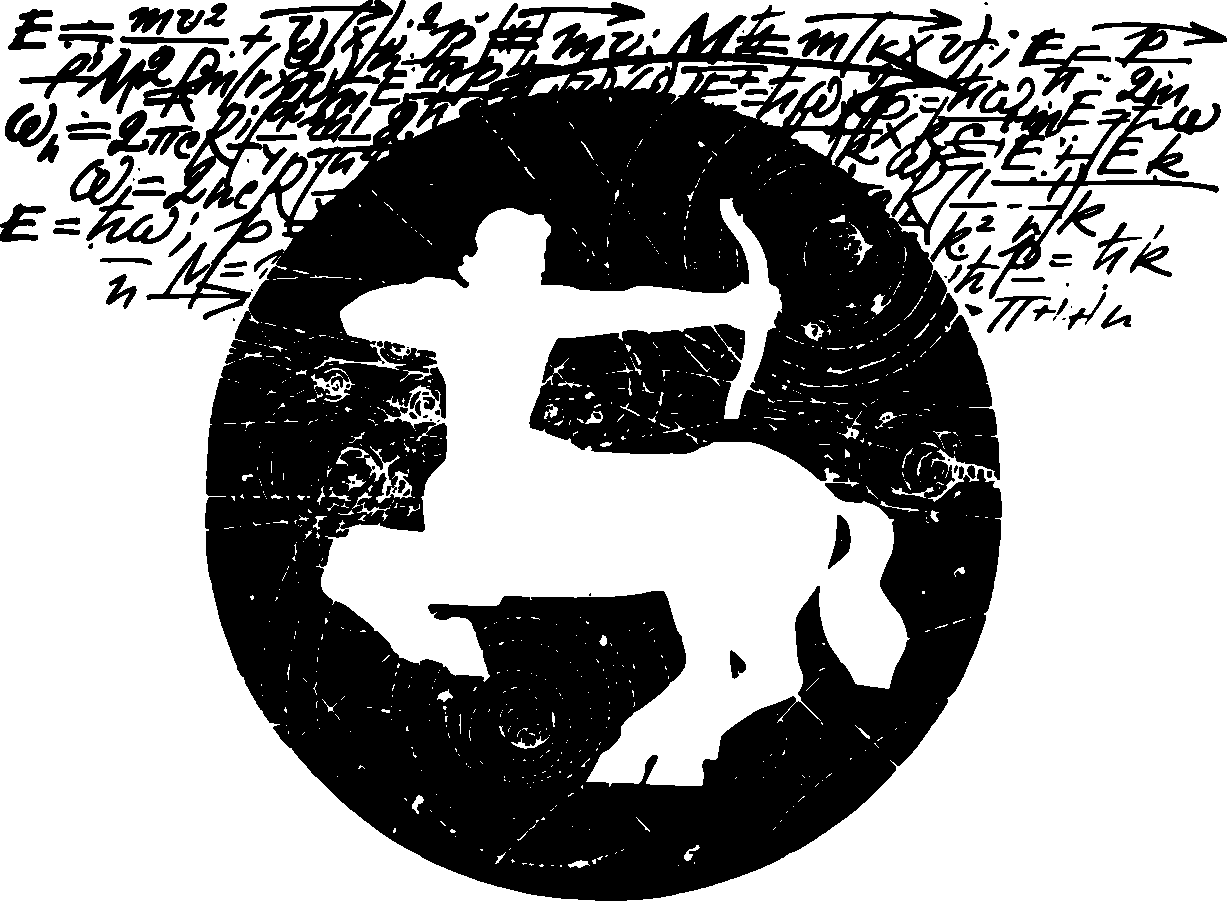
\includegraphics[width=\linewidth]{figures/ch-01.pdf}
\end{figure*}
\cleardoublepage
\section{Certain Characteristics and Properties of Microparticles}
\label{sec-01}

\emph{Molecules, \marginnote{Microparticles}atoms, atomic nuclei} and
\emph{elementary particles} belong to the category of microparticles. The list of elementary particles is at present fairly extensive and includes quanta of electromagnetic field (\emph{photons}) as well as two groups of particles, the \emph{hadrons} and the \emph{leptons}. Hadrons are characterized by a strong (nuclear) interaction, while leptons never take part in strong interactions. The electron; the muon and the two neutrinos (the electronic and muonic) are leptons. The group of hadrons is numerically much larger. It includes nucleons (proton and neutron), mesons (a group of particles lighter than the proton) and hyperons (a group of particles heavier than the neutron). With the exception of photons and some neutral mesons, all elementary particles have corresponding anti-particles. 

Among properties of microparticles, let us first mention the \emph{rest mass}
and \emph{electric charge}. As an example, we note that the mass $m$ of an
electron is equal to \SI{9.1d-28}{\gram}; a proton has mass equal to $1836m$, a neutron, $1839m$ and a muon, $207m$. Pions ($\pi$-mesons) have a mass of about $270m$ and kaons ($K$-mesons), about $970m$. The rest mass of a photon and of both neutrinos is assumed to be equal to zero.

The mass of a molecule, atom or atomic nucleus is equal to the sum of the masses of the particles constituting the given microparticle, less a certain amount known as the mass defect. The mass defect is equal to the ratio of the energy that must be expended to break up the microparticle into its constituent particles (this energy is usually called the binding energy) to the square of velocity of light. The stronger the binding between particles, the greater is the mass defect. Nucleons : in atomic nuclei have the strongest binding-the mass defect for one nucleon exceeds $10m$.

The magnitude of the electric charge of a microparticle is a multiple of the magnitude of the charge of an electron, which is equal to \SI{1.6d-19}{\coulomb} (\num{4.8d-10} CGSE units). Apart from charged microparticles, there also exist neutral microparticles (for example, photon, neutrino, neutron). The electric charge of a complex micro- particle is equal to the algebraic sum of the charges of its constituent particles.

Spin \marginnote{Spin of a Microparticle}is one of the most important
specific characteristics of a microparticle. It may be interpreted as
the angular momentum of the microparticle not related to its motion as
a whole (it is frequently known as the internal angular momentum of
the microparticle). The square of this angular momentum is equal to
$\hbar^{2}s (s + 1)$, where $s$ for the given microparticle is a
definite integral or semi-integral number (it is this number which is
usually referred to as the spin), $\hbar$ is a universal physical
constant which plays an exceptionally important role in quantum
mechanics. It is called \emph{Planck's constant} and is equal to
\SI{1.05d-34}{ \joule\second}. Spin $s$ of a photon is equal to 1,
that of an electron (or any other lepton) is equal to $\dfrac{1}{2}$
while pions and kaons don't have any spin.\sidenote{The definition of spin of a microparticle assumes that spin is independent of external conditions. This is true for elementary particles. However, the spin of an atom, for example, may change with a change in the state of the latter. In other words, the spin of an atom may change as a result of influences on the atom which lead to a change in its state.} 
Spin is a specific property of a microparticle. It does not have a
classical analogue and certainly points to the complex internal
structure of the microparticle. True, it is sometimes attempted to
explain the concept of spin on the 'model of an object rotating around
its axis (the very word ``spin'' means ``rotate). Such a mode is
descriptive but not true. In any case, it cannot be literally
accepted. The term ``rotating microparticl'' that one comes across in
the literature does not by any means indicate the rotation of the
microparticle, but merely the existence of a specific internal angular
momentum in it. In order that this momentum be transformed into
``classical'' angular momentum (and the object thereby actually
rotate) it is necessary to satisfy the conditions $s \gg 1$. Such a
condition, however, is usually not satisfied.

The peculiarity of the angular momentum of a microparticle is
manifested, in particular, in the fact that its projection in any
fixed direction assumes discrete values $\hbar s, \hbar (s -1 ),
\ldots , - \hbar s$, thus in total $2s + 1$ values. It means that the
microparticle may exist in $2s + 1$ spin states. Consequently, the
existence of spin in a microparticle leads to the appearance of
additional (internal) degrees of freedom.  

If we \marginnote{Bosons and Fermions}know the spin of a
microparticle, we can predict its behaviour in the collective of
microparticles similar to it (in other words, to predict the
statistical properties of the microparticle). It turns out that all
the microparticles in nature can be divided into two groups, according
to their statistical properties: a group with integral values of spin
or with zero spin, and another with half-integral spin.

Microparticles of the first group are capable of populating one and
the same state in unlimited numbers.\sidenote{The concept of the state
  of a microparticle is discussed in Section \ref{sec-03} below.} Moreover, the more
populated is a given state, the higher is the probability that a
microparticle appears in this state. Such microparticles are known to
obey the Bose-Einstein statistics, in short they are simply called
\emph{bosons}. Microparticles of the second group may inhabit the states
only one at a time, if the state under consideration is already
occupied, no other microparticle of the given type can be accommodated
there. Such microparticles obey Fermi-Dirac statistics and are called
\emph{fermions}.

Among elementary particles, photons and mesons are hosons while the
leptons (in particular, electrons), nucleons and hyperons are
fermions. The fact that electrons are fermions is reflected in the
well-known \emph{Pauli exclusion principle}.


All \marginnote{Instability of Microparticles}elementary particles
except the photon, the electron, the proton and both neutrinos are
\emph{unstable}. This means that they decay spontaneously, without any
external influence, and are transformed into other particles. For
example, a neutron spontaneously decays into a proton, an electron and
an electronic antineutrino 
\begin{equation*}
n \to p + e^{-} + \nu_{e}.
\end{equation*}
It is impossible to predict precisely at what time a particular
neutron will decay since each individual act of disintegration occurs
randomly. However, by following a large number of acts, we find a
regularity in decay. Suppose there are $N_{0}$ neutrons $(N_{0} \gg
1$) at time $t =0$. Then at the moment $t$ we are left with
\begin{equation*}
N (t) = N_{0} \exp \left(-\dfrac{t}{\tau} \right)
\end{equation*}
neutrons, where $\tau$ is a certain constant characteristic of
neutrons. It is called the lifetime of a neutron and is equal to
\SI{e3}{\second}. The quantity $\exp \left(-\dfrac{t}{\tau} \right)$
determines the probability that a given neutron will not decay in time $t$.  

Every unstable elementary particle is characterized by its
lifetime. The smaller the lifetime of a particle, the greater the
probability that it will decay. For example, the lifetime of a muon is
\SI{2.2d-6}{\second}, that of a positively charged $\pi$-meson is
\SI{2.6d-8}{\second}, while for a neutral $\pi$-meson the lifetime is
\SI{e-16}{\second} and for hyperons, \SI{e-10}{\second}. In recent
years, a large number of particles (about 100) have been observed to
have an anomalously small lifetime of about \SIrange{e-22}{e-23}{\second}. These
are called resonances. 

It is worth noting that hyperons and mesons may decay in different
ways. For example, the positively charged $\pi$-meson may decay into a
muon and a muonic neutrino 
\begin{equation*}
\pi^{+} \to \mu^{+} + \nu_{\mu}, 
\end{equation*}
into a positron (antielectron) and electronic neutrino
\begin{equation*}
\pi^{+} \to e^{+} + \nu_{e},
\end{equation*}
into a neutral rt-meson, positron and electronic neutrino
\begin{equation*}
\pi^{+} \to  \pi^{0} + e^{+} + \nu_{e}.
\end{equation*}


% \begin{align*}
% \pi^{+} & \to \mu^{+} + \nu_{\mu}, \\
% & \text{into a positron (antielectron) and electronic neutrino}\\
% \pi^{+} &\to e^{+} + \nu_{e},\\
% & \text{into a neutral rt-meson, positron and electronic neutrino}\\
% \pi^{+} & \to  \pi^{0} + e^{+} + \nu_{e}.
% \end{align*}

For any particular $\pi$-meson, it is impossible to predict not only
the time of its decay, but also the mode of decay it might
``choose''. Instability is inherent not only in elementary particles,
but also in other microparticles. The phenomenon of radioactivity
(spontaneous conversion of isotopes of one chemical element into
isotopes of another, accompanied by emission of particles) shows that
the atomic nuclei can also be unstable. Atoms and molecules in excited
states are also unstable; they spontaneously return to their ground
state or to a less excited state.

Instability determined by the probability laws is, apart from spin,
the second special specific property inherent in microparticles. This
may also be considered as an indication of a certain ``internal
complexity'' in the microparticles. 

In conclusion, we may note that instability is a specific, but by no
means essential, property of microparticles. Apart from the unstable
ones, there are many stable microparticles: the photon, the electron,
the proton, the neutrino, the stable atomic nuclei, as well as atoms
and molecules in their ground states.  

Looking at the decay scheme of a neutron \marginnote{Interconversion of
Microparticle}
\begin{equation*}
n \to  p + e^{-} + \overline{\nu}_{e}, 
\end{equation*}
an inexperienced reader might presume that a neutron is made up of
mutually bound proton, electron and electronic antineutrino. Such an
assumption is wrong. The decay of elementary particles is by no means
a disintegration in the literal sense of the word; it is just an act
of conversion of the original particle into a certain aggregate of new
particles; the original particle is annihilated while new particles
are created. The unfoundedness of the literal interpretation of the
term ``decay of particles'' becomes apparent when one considers that
many particles can decay in several different ways.  

The interconversion of elementary particles turns out to be much more
diverse and complicated if we consider particles not only in a free,
but also in a bound state. A free proton is stable, and a free neutron
decays according to the equation mentioned above. If, however, the
neutron and the proton are not free but bound in an atomic nucleus,
the situation radically changes. Now the following equations of
interconversion are operative: 
\begin{align*}
n &\to p + \pi^{-},\\
 p & \to n + \pi^{+} 
\end{align*}
(here, $\pi^{-}$ is a negatively charged $\pi$-meson, the antiparticle
of the $\pi^{+}$-meson). These equations very well illustrate that an
attempt to find out whether the proton is a ``constituent'' of the
neutron, or vice versa is pointless.  

Everyday experience teaches us that to break up an object into parts
means to reveal its structure. The idea of analysis (or splitting)
reflects the characteristic feature of classical methods. When we go
over to the microparticles, this idea still holds to a certain extent:
the molecules are made up of atoms, the atoms consist of nuclei and
electrons, the nuclei are made up of protons and neutrons. However,
the idea exhausts itself at this point: for example, ``splitting up'' of
a neutron or a proton does not reveal the structure of these
particles. As regards elementary particles, when we say that a
particle decays into parts, it does not mean that these particles
constitute the given particle. This condition itself might serve as a
definition of an elementary particle.  

Decay of elementary particles is not the only kind of interconversion
of particles. Equally important is the case of interconversion of
particles when they collide with one another. As an example, we shall
consider some equations of interconversion during collision of photons
($\gamma$) with protons and neutrons: 
\begin{align*}
\gamma  + p &\to n + \pi^{+}, \\
\gamma + n &\to p + \pi^{-}, \\
\gamma + p &\to p + \pi^{0},\\
\gamma + n &\to n +  \pi^{0},\\
 \gamma +p &\to p + \pi^{+} + \pi^{-},\\
 \gamma +n &\to n + \pi^{0} + \pi^{0},\\
\gamma +p &\to p + p + \overline{p} 
\end{align*}
(where $\overline{p}$-denotes an antiproton) It should be mentioned
here that in all the above equations, the sum of the rest masses of
the end particles is greater than the rest mass of the initial
ones. In other words, the energy of the colliding particles is
converted into mass (according to the well-known relation $E =
mc^{2}$). These equations demonstrate, in particular, the
fruitlessness of efforts to break up elementary particles (in this
case, nucleons) by ``bombarding'' them with other particles (in this
case, photons): in fact, it does not lead to a breaking-up of the
particles being bombarded at, but to the creation of new particles, to
some extent at the expense of the energy of the colliding particles.

A study of the interconversion of elementary particles permits us to
determine certain regularities. These regularities are expressed in
the form of laws of conservation of certain quantities which play the
role of some definite characteristics of certain particles. As a
simple example, we take the electric charge of a particle. For any
interconversion of particles, the algebraic sum of electric charges
of the initial and end particles remains the same. The law of
conservation of the electric charge refers to a definite regularity in
the interconversion of particles: it permits one to summarily reject
equations where the total electric charge is not conserved.  

\begin{fullwidth}
\setlength{\leftskip}{3cm}
\textsf{\small As a more complicated example, we mention the so-called barionic
charge of a particle. It has been observed that the number of nuleons
during an interconversion of particles is conserved. With the
discovery of antinucleons, it was observed that additional nucleons
may be created, but they must he created in pairs with these
antinucleons. So a new characteristic of particles, the barionic
charge, was introduced. It is equal to zero for photons, leptons and
mesons, +1 for nucleons, and -1 for antinucleons, This permits us to
consider the above-mentioned regularity as a law of conservation of
the total barlonic charge of the particles. The law was also confirmed
by the discoveries that followed: the hyperons were assigned a
barionic charge equal to 1 (as for nucleons) and the antihyperons were
given a barionic charge equal to -1 (as for antinucleons).}

\end{fullwidth}
\vspace{5pt}
\setlength{\leftskip}{0pt}

While going over from macroparticles to microparticles, one would
expect qualitatively different answers to questions like: Which
dynamic variables should be used to describe the state of the object?
How should its motion be depicted? Answers to these questions reveal
to a considerable extent the specific nature of microparticles. In
classical physics, we make use of the \emph{laws of conservation of
  energy, momentum and angular momentum}. It is well known that these
laws are consequences of certain properties of the symmetry of space
and time. Thus, the law of conservation of energy is a consequence of
\emph{homogeneity of time}. (independence of the course of a physical
process of the moment chosen as the starting point of the process);
the law of conservation of momentum is a consequence of the
\emph{uniformity of space} (all points in space are physically
equivalent); the law of conservation of angular momentum is a
consequence of the \emph{isotropy of space} (all directions in space
are physically equivalent). To elucidate the properties of symmetry of
space and time, we note, for example, that thanks to these properties,
Kepler's laws describing the motion of the planets around the sun are
independent of the position of the sun in the galaxy, of the
orientation in space of the plane of motion of the planets and also of
the century in which these laws were discovered. The connection
between the properties of symmetry of space and time and the
corresponding conservation laws means that the energy, momentum and
angular momentum can be considered as \emph{integrals of motion},
whose conservation is a consequence of the corresponding homogeneity
of time and the homogeneity and isotropy of space.

The absence of any experimental evidence indicating violation of the
above-mentioned properties of symmetry of space and time for
microphenomena reveals that such dynamic parameters as energy,
momentum and angular momentum should retain their meaning when applied
to microparticles. In other words, the connection of these dynamic
variables with the fundamental properties of symmetry in space and
time makes them universal variables, i.e. variables which are ``used''
while considering the kind of phenomena occurring in different
branches of physics.

When transferring the concepts of energy, momentum and angular
momentum from classical physics to quantum mechanics, however, the
specific nature of the microparticles must be taken into account. In
this connection we recall the well-known expressions for energy ($E$),
momentum ($\vec{p}$) and angular momentum ($\vec{M}$) of a classical
object, having mass $m$, coordinate $\vec{r}$, velocity $\vec{v}$:
\begin{equation}%
\left.
\begin{split}
E & = \frac{mv^{2}}{2} +U(\vec{r}) \\
 \vec{p}& = m\vec{v} \\
\vec{M} & =m(\vec{r} \times \vec{v})
\end{split}
\quad \quad \right\}
\label{eq-1.1}
\end{equation}

Eliminating the velocity, we get from here the relations connecting
energy, momentum and angular momentum of a classical object:
\begin{align}%
%\begin{split}
E & = \frac{p^{2}}{2m} +U(\vec{r})\label{eq-1.2}\\
\vspace{8pt}
%\end{split}
%\begin{split}
\vec{M} & = m(\vec{r} \times \vec{p}) \label{eq-1.3}
%\end{split}
\end{align}
If we turn to a microparticle, we can go a bit farther, (see Section \ref{sec-03})
and conclude that relations (\ref{eq-1.2}) and (\ref{eq-1.3}) are no
longer valid. In other words, the classical connections between the
integrals of motion become useless as we go over to microparticles (as
regards relations (\ref{eq-1.1}), they cannot be mentioned at all
since the very concept of the velocity of a microparticle, as we shall
see below, is meaningless). This is the first qualitatively new
circumstance.  

In order to consider the other qualitatively new circumstances, we
must turn to the fundamental ideas of quantum mechanics, i.e. the idea
of \emph{quantization of physical quantities} and the idea of wave-particle
duality.

\section{Two Fundamental Ideas of Quantum Mechanics}
\label{sec-02}

The essence \marginnote{The Idea of Quantization (Discreteness)}of the
idea of quantization lies in the fact that certain physical quantities
related to the microparticles may assume, under relevant
circumstances, only certain \emph{discrete values}. These quantities are said
to be \emph{quantized}. 

Thus the energy of any microparticle in a bound state, like that of an
electron in an atom, is quantized. The energy of a freely moving
microparticle, however is not quantized.

\begin{marginfigure}%[cm]
\centering
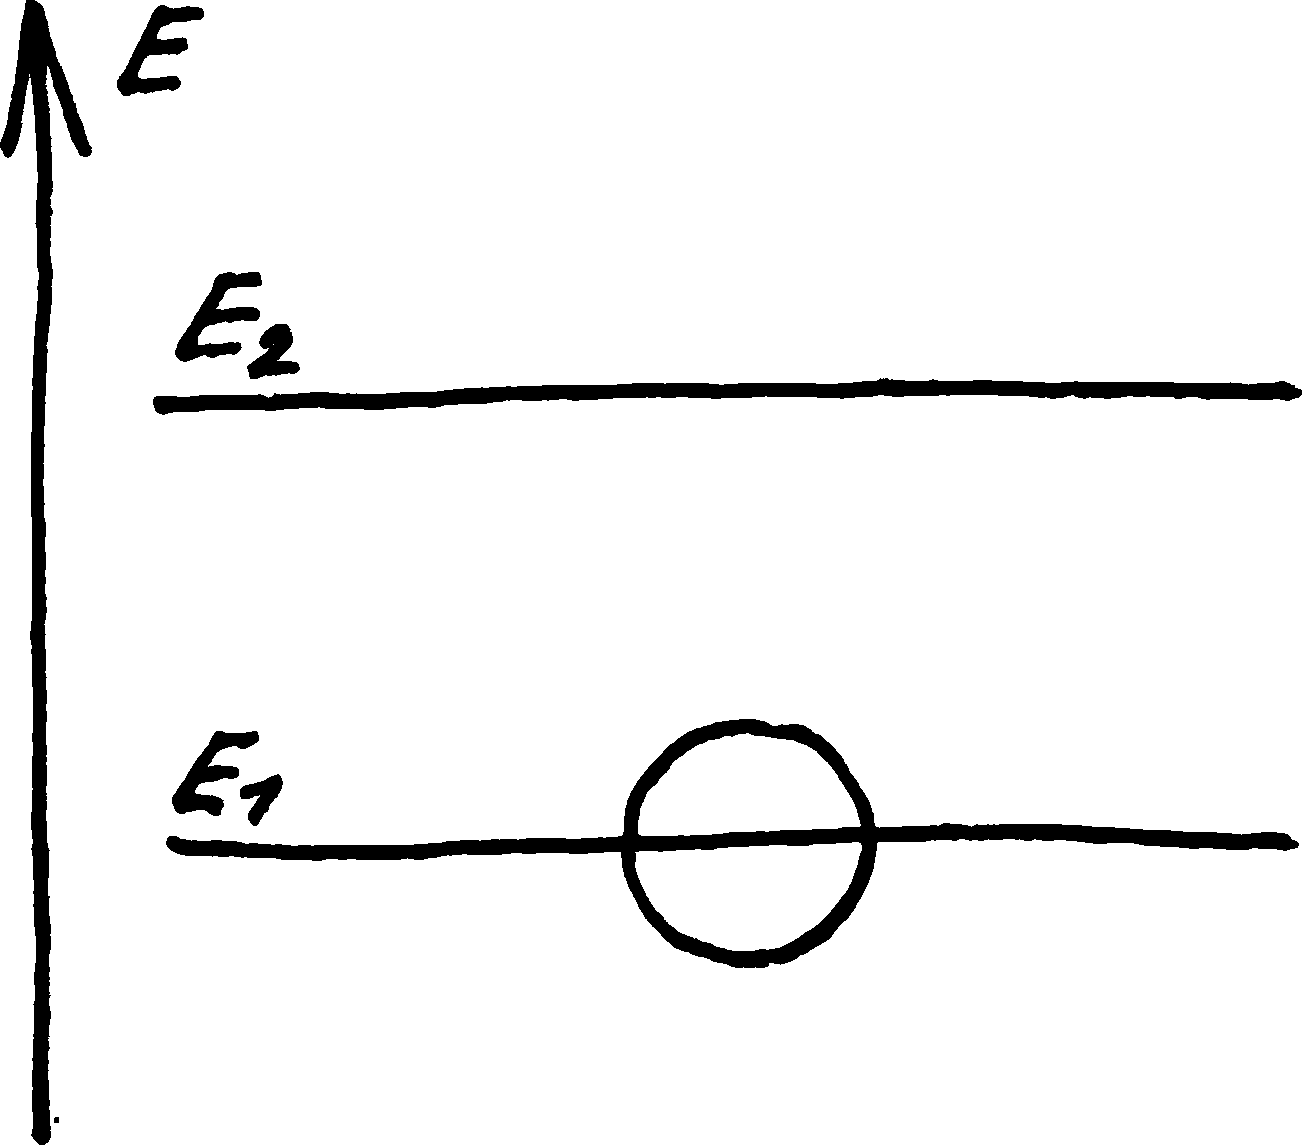
\includegraphics[width=0.9\linewidth]{figures/fig-02-01.pdf}
\caption{Energy levels of an electron and quantum transition.}
\label{fig-2.1}
\end{marginfigure}

Let us consider the energy of an electron in an atom. The system of
so-called energy levels corresponds to a discrete set of values of
electron energy. We consider two energy levels $E_{1}$ and $E_{2}$ as
shown in Figure \ref{fig-2.1} (the values of electron energy are
plotted along the vertical axis). The electron may possess energy
$E_{1}$ or $E_{2}$ and cannot possess any intermediate energy-all
values of energy $E$ satisfying the condition $E_{1} < E < E_{2}$ are
forbidden for it\sidenote{A specific situation in quantum mechanics is
  possible in which one must assume that an electron occupies level
  $E_{1}$ as well as level $E_{2}$ (see Section \ref{sec-10}).}. It
should be noted that the discreteness of energy does not mean in any
case that the electron is ``doomed'' to remain forever in the initial
energy state (for example on level $E_{1}$) . The electron may go over to
another energy state (level $E_{2}$ or any other) by acquiring or releasing
the corresponding amount of energy. Such a transition is called a
\emph{quantum transition}.

The quantum-mechanical idea of discreteness has a fairly long
history. By the end of 19$^{\text{th}}$ century, it was established that the
radiation spectra of free atoms are \emph{line spectra} (i.e. they consist of
sets of lines) and contain, for every element, definite lines which
form ordered groups (\emph{series}). In 1885, it was discovered that atomic
hydrogen emits radiation of frequencies $\omega_{n}$ (henceforth we use the
cyclic frequencies $\omega$, related to the normal frequencies $\nu$ through the
equation $\omega = 2 \pi \nu$) which may be described by the formula
\begin{equation}%
\omega_{n} = 2 \pi c R \left( \frac{1}{4} - \frac{1}{n^{2}} \right)
\label{eq-2.1}
\end{equation}

where $n$ are integral numbers $3, 4, 5, \ldots$, $c$ is the velocity
of light, $R$ is the so-called \emph{Rydberg constant} ($R =
\SI[per-mode=symbol]{1.097d7}{\per\meter}$). Formula (\ref{eq-2.1}) was
derived by Balmer, hence the set of frequencies described by this
formula is called the \emph{Balmer series}. The frequencies of the Balmer
series fall in the visible region of spectrum. Later (in the beginning
of 20$^{\text{th}}$ century), additional series of radiation from atomic hydrogen
falling in the ultraviolet and infrared regions were discovered. The
regulari- ties in the structure of these spectra were identical to the
regularities in the structure of the Balmer series, which enabled a
generalization of formula (\ref{eq-2.1}) in the following form: 
\begin{equation}%
\omega_{n} = 2 \pi c R \left( \frac{1}{k^{2}} - \frac{1}{n^{2}} \right)
\label{eq-2.2}
\end{equation}

The number $k$ fixes the series (in each series $n > k$); $k = 2$
gives the Balmer series, $k = 1$, the Lyman series (ultraviolet
frequencies), $k = 3$, the Paschen series (infrared frequencies), and
so on.  

Regularity in the structure of series was observed not only in the
spectrum of atomic hydrogen, but also in the spectra of other
atoms. It definitely indicated the possibility of some
generalizations. One such generalization was proposed by Ritz in 1908
in his \emph{combination principle}, which states that if the formulae of
series are given and the constants occurring in them are known, any
newly discovered line in the spectrum may be obtained from the lines
already known by means of combinations in the form of sums and
differences. This principle may be applied to hydrogen in the
following way: we write the so-called spectral terms for different
numbers $n$: 
\begin{equation*}
T(n) = \frac{2 \pi c R}{n^{2}} 
\end{equation*}

Then each frequency observed in the hydrogen spectrum may be expressed
as a combination of two spectral terms. By combining the spectral
terms, it is possible to predict different frequencies. 

It is remarkable that at about the same time, the idea of discreteness
arose in another direction (not related to atomic spectroscopy). This
is the case of radiation within a closed volume or, in other words,
\emph{black body radiation}. After analyzing the experimental data, Planck in
1900 proposed his famous hypothesis. He suggested that the energy of
electromagnetic radiation is emitted by the walls of a cavity not
continuously, but in \emph{portions} (\emph{quanta}), the energy of a
quantum being equal to 
\begin{equation}%
E = \hbar \omega 
\label{eq-2.3}
\end{equation}
where $\omega$ is the frequency of radiation and $\hbar$
is a certain universal constant (it later became known as Planck's
constant). Planck's hypothesis provided an agreement between the
theory and experiment and, in particular, removed the flaws arising in
the previous theory when passing to higher frequencies. This had been
called the ``ultraviolet catastrophe'' (see, for example, Volume 3 of
Savelyev's General Physics). \cite[-1cm]{savelyev-1980}

In 1913\marginnote{The Idea of Quantization and Bohr's Model of
  Hydrogen Atom}, Bohr proposed his theory of the hydrogen atom. This
theory was evolved as a ``confluence'' of the planetary atomic model
by Rutherford, the Ritz combination principle, and Planck's ideas of
quantization of energy.

According to Bohr's theory, there exist certain states in which the
atom does not radiate (\emph{stationary states}). The energy of these
states forms a \emph{discrete spectrum}, $E_{1}, E_{2}, \ldots,
E_{n}$. The atom emits (absorbs) during transition from one stationary
state to another. The emitted (absorbed) energy is the difference
between the energies of the corresponding stationary states. Thus,
during a transition from the state with energy $E_{n}$ to the state with
lower energy$ E_{k}$ , a quantum of radiation with energy $(E_{n} - E_{k})$ is
emitted. Thus a line with frequency 
\begin{equation}%
\omega = \frac{E_{n}- E_{k}}{\hbar} 
\label{eq-2.4}
\end{equation}
appears in the spectrum. Formula (\ref{eq-2.4}) expresses the
well-known Bohr's frequency condition.

In Bohr's theory, the $n$-th stationary state of hydrogen
atom corresponds to a circular orbit of radius $r_{n}$ along which the
electron revolves around the nucleus. In order to compute $r_{n}$ , Bohr
suggested, firstly, using Newton's second law for a charge moving in a
circle under the influence of a Coulomb's force: 
\begin{equation}%
m \frac{v_{n}^{2}}{r_{n}} = \frac{e^{2}}{r_{n}^{2}}
\tag{2.5a}
\label{eq-2.5a} 
\end{equation}
(here $m$ and $e$ are the mass and the charge of an electron,
$v_{n}$ is the velocity of the electron in the $n$-th
orbit). Secondly, Bohr suggested the condition of quantization of the
angular momentum of the electron: 
\begin{equation}%
  m v_{n} r_{n} = n \hbar
\tag{2.5b}
\label{eq-2.5b} 
\end{equation}
By using relations (\ref{eq-2.5a}) and (\ref{eq-2.5b}), it is easy to
find $r_{n}$ and $v_{n}$:
\addtocounter{equation}{1}
\begin{equation}%
\begin{split}
r_{n} & = \left( \frac{\hbar^{2}}{me^{2}} \right) n^{2}\\
v_{n} & = \frac{e^{2}}{\hbar n}
\end{split}
\label{eq-2.6} 
\end{equation}

The energy $E_{n}$ of the stationary state consists of kinetic ($T_{n}$) and
potential ($U_{n}$) terms: 
\begin{equation*}
E_{n} = T_{n} + U_{n}
\end{equation*}
Assuming that $T_{n} = \frac{mv_{n}^{2}}{2}, \,\, U_{n} =
-\frac{e^{2}}{r_{n}}$ and using (\ref{eq-2.6}), we find that
\begin{equation}%
E_{n} = - \frac{me^{4}}{2 \hbar^{2} n^{2}}
\label{eq-2.7}
\end{equation}

The negative sign of the energy means that the electron is in a bound
state (energy of a free electron is taken to be equal to zero).

Substituting the result (\ref{eq-2.7}) into the frequency
relation (\ref{eq-2.4}), and comparing the expression thus obtained with
formula (\ref{eq-2.2}), we may, following Bohr, find an expression for
Rydberg's constant: 
\begin{equation}%
 R = \frac{me^{4}}{4 \pi c \hbar^{3}}
\label{eq-2.8} 
\end{equation}

Bohr's theory (or the old quantum theory, as it is now called)
 suffered from internal contradictions; in order to determine the
 radius of the orbit, one had to make use of relations of different
 kinds-the classical relation (\ref{eq-2.5a}), and the quantum relation
 (\ref{eq-2.5b}). In spite of this, the theory was of great significance as a
 first step towards the creation of a consistent quantum
 theory. Moreover, the nature of the spectral terms, and,
 consequently, the Ritz combination principle, was revealed for the
 first time and the calculated value of Rydberg's constant was in
 excellent agreement with its empirical value. The success of the
 theory proved testimony to the usefulness of the idea of
 quantization. Having acquainted himself with Bohr's calculations,
 Sommerfeld wrote Bohr a letter, in which he said: 

\begin{quote} 
I thank you very much for sending me your extremely interesting
work~\ldots \,\, The problem of expressing the Rydberg-Ritz constant by
Planck's has been for some time in my thoughts \ldots \,\, Although I am
for the present still rather sceptical about atom models in general,
nevertheless the calculation of the constant is indisputably a great achievement.
\end{quote}

We must note that in contrast to energy, the angular momentum of a
microparticle is always quantized. Thus, the observed values of the
square of angular momentum of a microparticle are expressed by the
formula
\begin{equation}%
 M^{2}= \hbar^{2} l (l+1), 
\tag{2.9a}
\label{eq-2.9a} 
\end{equation}
where $l$ is an integer $0, 1, 2, \ldots$ \marginnote{On Quantization
  of Angular Momentum}. If we consider the angular momentum of an
electron in the atom in the $n$-th stationary state, the number $l$
assumes values from 0 to $n-1$.  

In the literature, it is customary to refer to the angular momentum as
simply \emph{momentum}, Henceforth, we shall follow this practice.

The projection of the momentum of a microparticle in a certain
direction (let us denote it as $z$-direction) assumes the values 
\begin{equation}%
 M_{z}= \hbar m
\tag{2.9b}
\label{eq-2.9b} 
\end{equation}

where $m=-l,-l+1, \ldots ,l-1,1$. For a given value of the number $l$,
the number $m$ can assume $2l + 1$ discrete values. We emphasize here
that different projections of the momentum of a microparticle in a
given direction differ from one another by values which are multiples
of Planck's constant.

It was mentioned above that spin is a distinctive ``internal''
momentum of a microparticle having a definite value for a given
microparticle. To distinguish it from the \emph{spin} momentum,
ordinary momentum is called \emph{orbital} momentum. Kinematically the
spin momentum is analogous, to the orbital momentum. Naturally, in
order to find the possible projections of the spin momentum we must
use a formula of the type (\ref{eq-2.9b}) (as in the case of orbital
momentum, the projections of the spin momentum differ from one another
by integral multiples of Planck's constant). If $s$ is the spin of a
microparticle (this number was introduced in Section \ref{sec-01}),
then the projection of the spin momentum assumes values $\hbar
\sigma$, where $\sigma = -s,-s+1, \ldots s- 1, s $. Thus, the
projection of the spin of an electron assumes values $-
\dfrac{\hbar}{2}$ and $+ \dfrac{\hbar}{2}$. The numbers $n, l, m,
\sigma$ considered here determine the different discrete values of the
quantized dynamic variables (in this case, energy and momentum), and
are called \emph{quantum numbers}; $n$ is called the \emph{principal}
quantum number; $l$, the \emph{orbital} quantum number; $m$, the
\emph{magnetic} quantum number and $\sigma$, the \emph{spin} quantum
number. There also exist other quantum numbers.

In spite of \marginnote{Anomalies of Quantum Transitions}the
resounding success of Bohr's theory, the idea of quantization
engendered serious doubts in the beginning. It was noticed that the
idea was full of internal contradictions. Thus in his letter to
Bohr, Rutherford [19] wrote in 1913: 
\begin{quote}
  ...Your ideas as to the mode of origin of the spectrum of hydrogen
  are very ingenious and seem to work out well; but the mixture of
  Planck's ideas with the old mechanics makes it very difficult to
  form a physical idea of what is the basis of it. There appears to me
  one grave difficulty in your hypothesis which I have no doubt you
  fully realise namely, how does an electron decide what frequency it
  is going to vibrate at when it passes from one stationary state to
  the other? It seems to me that you would have to assume that the
  electron knows beforehand where it is going to stop\sidenote{The
    reader should not be confused by the remarks about the
    oscillations of electron: uniform motion in a eircle is a
    superposition of two harmonic oscillations in mutually
    perpendicular directions.}...
\end{quote}

We shall explain the difficulties noticed by Rutherford. Let an
electron occupy level $E_{1}$ (Figure \ref{fig-2.1}). In order to go
over to the level $E_{2}$, the electron must absorb a quantum of
radiation (i.e, a photon) with a definite energy equal to ($E_{2} - E_{1}$). Absorption of a photon with any other energy will not result
in the indicated transition and is therefore not possible (for
simplicity, we shall consider only two levels). The question now
arises: In what way does an electron perform a ``selection'' of the
``required'' photon out of the photon flux of different energies falling
on it? In order to ``select'' the ``required'' photon, the electron must
be ``previously aware'' of the second level, i.e. as if it had already
visited it. However, in order to visit the second level, the electron
must have first absorbed the ``required'' photon. This gives rise to a
vicious circle.  


\begin{fullwidth}
  \setlength{\leftskip}{3cm} \textsf{\small Further contradictions are
    observed while considering the jump of an electron from one orbit
    in the atom to another. Whatever the speed at which the transition
    of the electron from the orbit of one radius to that of another
    takes place, it has to last for some finite period of time
    (otherwise it would he a violation of the basic requirements of
    the theory of relativity). But then it is hard to understand what
    the energy of the electron should be during this intermediate
    period - the electron no longer occupies the orbit corresponding to
    energy $E_{1}$ and has not yet arrived at the orbit corresponding to
    energy $E_{2}$}
\end{fullwidth}
\vspace{5pt}
\setlength{\leftskip}{0pt}

It is thus not surprising that at one time efforts were made to obain
an explanation of experimental results without resorting to the idea
of quantization. In this respect, the famous remarks by Schr\"odinger
about ``these damned quantum jumps'', which, of course, were made in the
heat of the moment, are worth noting.

However, experience inevitably pointed to the usefulness of
quantization and no place was left for an alternative.

In this case, there is just one way out: new ideas must be introduced,
which form a non-contradictory picture of the whole including the
ideas of discreteness. The idea of wave-particle duality was just such
a new physical concept.

Classical physics \marginnote{Idea of Wave-Particle Duality} acquaints
us with two types of motion: \emph{corpuscular} and \emph{wave}
motion. The first type is characterized by a localization of the
object in space and the existence of a definite trajectory of its
motion. The second type, on the contrary, is characterized by
delocalization in space. No localized object corresponds to the motion
of a wave, it is the motion of a medium. In the world of
macrophenomena, the corpuscular and wave motions are clearly
distinguished. The motion of a stone thrown upward is something
entirely different from the motion of a wave breaking a beach.

These usual concepts, however, cannot be transferred to quantum
mechanics. In the world of microparticles, the above-mentioned strict
demarcation between the two types of motion is considerably
obliterated. The motion of a microparticle is characterized
simultaneously by wave and corpuscular properties. If we schematically
consider the classical particles and classical waves as two extreme
cases of the motion of matter, microparticles must occupy in this
scheme a place somewhere in between. They are not ``purely'' (in the
classical sense) corpuscular, and at the same time they are not
``purely'' wavelike; they are something qualitatively different. It may
be said that a microparticle to some extent is akin to a corpuscle,
and in some respect it is like a wave. Moreover, the extent depends,
in particular, on the conditions under which the microparticle is
considered. While in classical physics a corpuscle and a wave are two
mutually exclusive extremities (either particle, or wave), these
extremities, at the level of microphenomena, combine dialectically
within the framework of a single microparticle. This is known as
\emph{wave-particle duality}.

The idea of duality was first applied to electromagnetic radiation. As
early as 1917, Einstein suggested that quanta of radiation, introduced
by Planck, should be considered as particles possessing not only a
definite energy, but also a definite momentum: 
\addtocounter{equation}{1}
\begin{equation}%
\left.
\begin{split}
E & = \hbar \omega\\
p & = \frac{\hbar \omega}{c}
\end{split}
\quad \quad \right\}
\label{eq-2.10} 
\end{equation}
Later (from 1923), these particles became known as \emph{photons}.  

\begin{fullwidth}
  \setlength{\leftskip}{3cm} \textsf{\small The corpuscular properties of radiation were very clearly demonstrated
in the Compton effect (1923). Suppose a beam of X-rays is scattered by
atoms of matter. According to classical concepts, the scattered rays
should have the same wavelength as the incident rays. However,
experiment shows that the wavelength of scattered waves was greater
than the initial wavelength of the rays. Moreover, the difference
between the wavelengths depends on the angle of scattering. The
Compton effect was explained by assuming that the X-ray beam behaves
like a flux of photons which undergo elastic collisions with the
electrons of the atoms, in conformity with the laws of conservation of
energy and momentum for colliding particles. This led not only to a
qualitative but also to a quantitative agreement with experiment
(see [17]).}
\end{fullwidth}
\vspace{5pt}
\setlength{\leftskip}{0pt}


In 1924, de Broglie suggested that the idea of duality should be
extended not only to radiation but also to all microparticles. He
proposed to associate with every microparticle \emph{corpuscular
  characteristics} (energy $E$ and momentum $p$) on the one hand and
\emph{wave characteristics} (frequency $\omega$ and wavelength
$\lambda$) on the other hand. The mutual dependence between the
characteristics of different kinds was accomplished, according to de
Broglie, through the Planck's constant it in the following way:
\begin{equation}%
\left.
\begin{split}
E & = \hbar \omega\\
p & = \frac{ 2 \pi \hbar}{\lambda}
\end{split}
\quad \quad \right\}
\label{eq-2.11} 
\end{equation}
(the second relation is known as \emph{de Broglie's equation}). For
photons, relation (\ref{eq-2.11}) is automatically satisfied if we
substitute $\omega = \dfrac{2 \pi c}{\lambda}$ in (\ref{eq-2.10}). The
boldness of de Broglie's hypothesis lays in that relation
(\ref{eq-2.11}) was assumed to be satisfied not only for photons, but
gen- erally for all microparticles, and in particular, for those which
have a rest mass and which were hitherto associated with corpuscles.

De Broglie's ideas received confirmation in 1927, with the discovery
of \emph{electron diffraction}. While studying the passage of
electrons through thin foils, Davisson and Germer (as well as
Tartakovsky) observed characteristic diffraction rings on the detector
screen. For ``electron waves'' the crystal lattice of the target served
as a diffraction grating. Measurement of distances between
diffraction rings for electrons of a given energy confirmed de
Broglie's formula.

In 1949, Fabrikant and coworkers set up an interesting
experiment. They passed an extremely weak electron beam through the
diffraction apparatus. The interval between successive acts of passage
(between two electrons) was more than \num{e4} times longer than the
time required for the passage of an electron through the
apparatus. This ensured that other electrons of the beam do not
influence the behaviour of an electron. The experiment showed that for
a prolonged exposure, permitting registration of a large number of
electrons on the detector screen, the same diffraction pattern was
observed as in the case of regular electron beams. It was thus
concluded that the wave nature of the electrons cannot be explained as
an effect of the electron aggregate; every single electron possesses
wave properties.

The idea of quantization \marginnote{The Role of Planck's Constant}
introduces discreteness, and discreteness requires a unit of
measure. Planck's constant plays the role of such a measure. It may be
said that this constant determines the ``boundary'' between
microphenomena and macrophenomena. By using Planck's constant, as well
as mass and charge of an electron, we may form the following simple
composition having dimensions of length:
\begin{equation}%
r_{1} = \frac{\hbar^{2}}{me^{2}} = \SI{0.53d-8}{\centi\meter}
\label{eq-2.12} 
\end{equation}
(note that $r_{1}$ is the radius of the first Bohr orbit). According
to (\ref{eq-2.12}), a magnitude of about \SI{e-8}{\centi\meter} may be
considered as the spatial ``boundary'' of microphenomena. This is just
about the linear dimensions of an atom.

If the Planck constant Ii were, say, 100 times larger, then (other
conditions being equal) the ``limit'' of microphenomena would,
according to (\ref{eq-2.12}), have been of the order of
\SI{e-4}{\centi\meter}. This would mean that the microphenomena
would become much closer to us, to our scale, and the atoms would have
been much bigger. In other words, matter in this case would have
appeared much ``coarser'', and classical concepts would have to be
revised on a much larger scale.

As was indicated above, the projections of the momentum of a
microparticle differ from one another by multiples of $\hbar$ [see
(\ref{eq-2.9b})]. Consequently, Planck's constant appears here as a
\emph{unit of quantization}. If the orbital momentum is much greater
than $\hbar$, its quantization may be neglected. We get in this case the
classical angular momentum. In contrast to the orbital momentum, spin
momentum cannot be very large. It is clear, that it is impossible to
neglect its quantization in principle; hence the spin momentum does
not have a classical analogue (this circumstance was already
indicated in Section \ref{sec-01}).

Planck's constant is inseparably linked not only with the
 idea of quantization, but also with the idea of duality. From (\ref{eq-2.11})
 it is evident that this constant plays a fairly important role - it
 supplies a ``link'' between the corpuscular and wave properties of a
 microparticle. This becomes quite clear if we rewrite (\ref{eq-2.11}) in a
 form permitting us to take account of the vector nature of momentum:
\begin{equation}%
\left.
\begin{split}
E & = \hbar \omega\\
\vec{p} & = \hbar \vec{k}
\end{split}
\quad \quad \right\}
\label{eq-2.13} 
\end{equation}
Here $\vec{k}$ is the wave vector; its direction coincides with the
direction of propagation of the wave, and its magnitude is expressed
through the wavelength in the following way: 
\begin{equation*}
k = \frac{2 \pi}{\lambda} 
\end{equation*}
The left-hand sides of equations (\ref{eq-2.13}) describe corpuscular
properties of a microparticle, and the right-hand sides wave
properties. We note, by the way, that the form of relations (\ref{eq-2.13})
indicates the relativistic invariance of the idea of duality.

Thus, Planck's constant plays two fundamental roles in quantum
mechanics - it serves as a measure of discreteness, and it combines
the corpuscular and wave aspects of the motion of matter. The fact
that the same constant plays both these roles is an indirect
indication of the internal unity of the two fundamental ideas of
quantum mechanics.

In conclusion, we remark that the presence of Planck's constant in any
expression indicates the ``quantum-mechanical nature'' of this
expression.\sidenote[][-1cm]{The converse statement is not true. It would be
  incorrect to attempt, as is sometimes done, to reduce the whole
  ``essence'' or quantum mechanics to the presence of Planck's
  constant. This question is considered in [51].}
 
\section{Uncertainty Relations}
\label{sec-03}
Let us \marginnote{Idea of Duality and Uncertainty Relations}consider
an aggregate of a large number of plane waves (the nature of waves is
not important) propagating, say, along the $z$-axis. Let the frequencies
of the waves be ``spread'' over a certain interval $\Delta \omega$), and the values
of the wave vector, over an interval $\Delta k_{x}$. If all these plane waves are
superimposed on one another, we get a wave formation limited in space
called a \emph{wave packet} (Figure \ref{fig-3.1}). The spreading of the wave packet in
space ($\Delta x$) and in time ($\Delta t$) is determined by the
relations 
\begin{equation}%
\left.
\begin{split}
\Delta \omega \Delta t & \geqslant 1  \\
\Delta k_{x} \Delta x  & \geqslant 1
\end{split}
\quad \quad \right\}
\label{eq-3.1}
\end{equation}
\begin{marginfigure}[1cm]
\centering
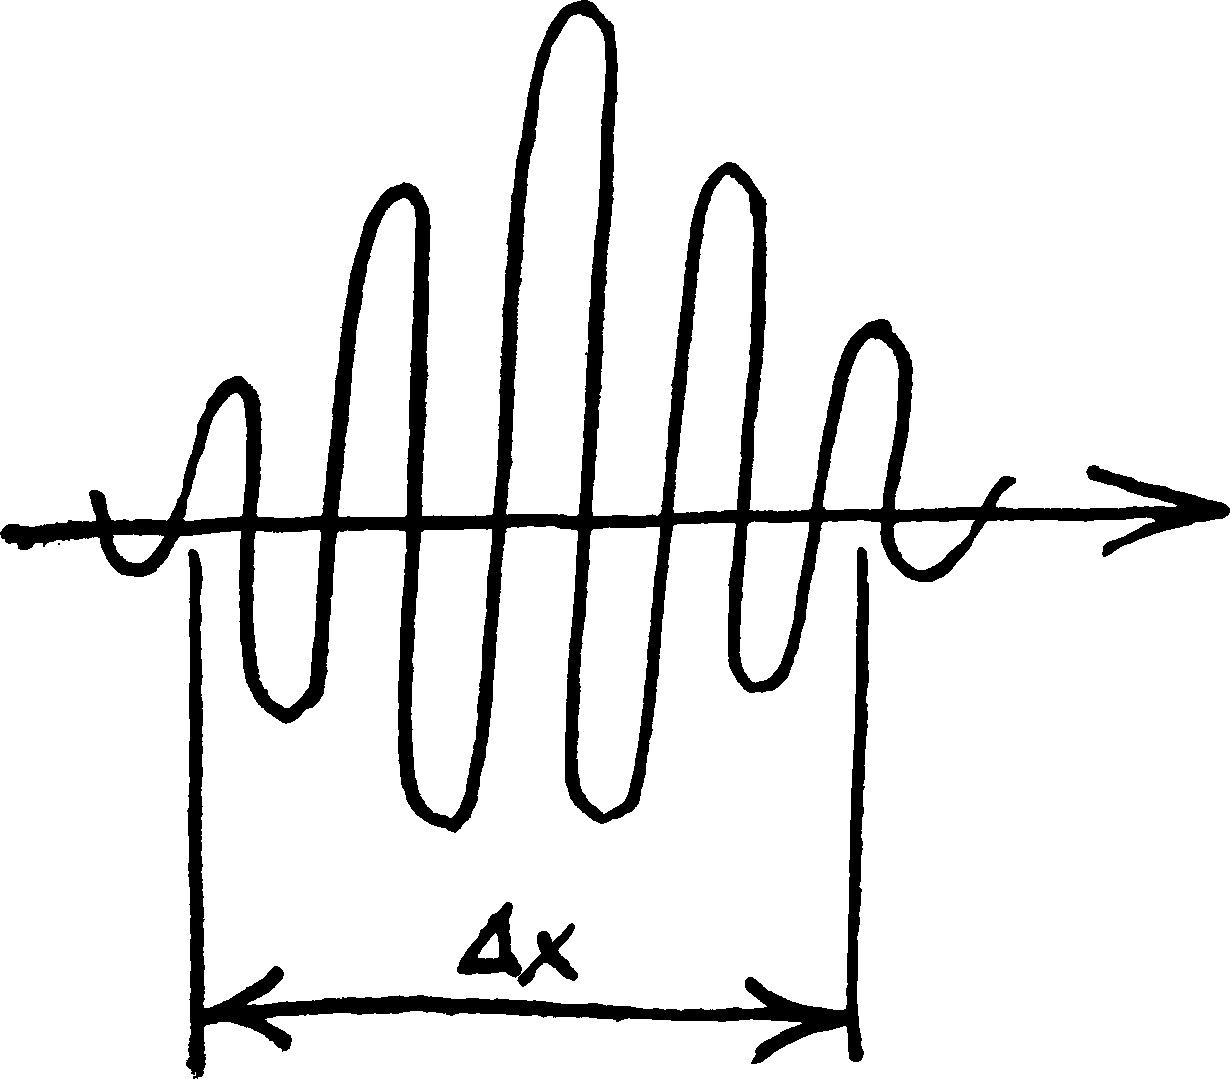
\includegraphics[width=\linewidth]{figures/fig-03-01.pdf}
\caption{The wave packet.}
\label{fig-3.1}
\end{marginfigure}
These relations are well known in classical physics. Those acquainted
with radio engineering know that for a more localized signal one must
take more plane waves with different frequencies. In other words, to
reduce $\Delta x$ and $\Delta t$, one must increase $\Delta k_{x}$ and
$\Delta \omega$.  

Digressing from the wave packet, we shall formally assume that
relations (\ref{eq-3.1}) are valid not only for classical waves, but
also for wave characteristics of a microparticle. We stress that this
assumption by no means indicates that we shall in fact model a
microparticle in the form of a wave packet. By considering $\omega$ and $k_{x}$
in (\ref{eq-3.1}) as wave characteristics of a microparticle and making use of
relations (\ref{eq-2.13}), it is easy to go over to an analogous expression for
the corpuscular characteristics of a microparticle (for its energy
and momentum): 
\begin{align}%
%\begin{split}
\Delta E \Delta t &  \geqslant \hbar \label{eq-3.2}\\
\vspace{8pt}
%\end{split}
%\begin{split}
\Delta p_{x} \Delta x &  \geqslant \hbar \label{eq-3.3}
%\end{split}
\end{align}

These relations were first introduced by Heisenberg in 1927 and are
called \emph{uncertainty relations}. Relations (\ref{eq-3.2}) and
(\ref{eq-3.3}) should be supplemented by the following uncertainty
relation:
\begin{equation}
\Delta M_{x} \Delta \varphi_{x}  \geqslant \hbar
\label{eq-3.4}
\end{equation}
where $\Delta \varphi_{x}$ is the uncertainty in the angular
coordinates of the microparticle (we consider rotation around the
$x$-axis) and $\Delta M_{x}$ is the uncertainty in the projection of
the momentum on the $x$-axis\sidenote{Notice that relations
  (\ref{eq-3.4}) and (\ref{eq-3.4a}) are valid only for small values
  of the uncertainty in angular coordinate ($\Delta \varphi \ll 2
  \pi$) or, in other words, for large values of uncertainty in the
  projection of the momentum.}.

By analogy with (\ref{eq-3.3}) and (\ref{eq-3.4}), one may write down relations for
other projections of momentum and angular momentum:
\begin{align}%
%\begin{split}
\Delta p_{x} \Delta x &  \geqslant \hbar, \quad \quad  \,\,\,\, \Delta p_{x}
\Delta x  \geqslant \hbar, \tag{3.3a} \label{eq-3.3a}\\
\vspace{8pt}
%\end{split}
%\begin{split}
\Delta M_{x} \Delta \varphi_{x} & \geqslant \hbar, \quad \quad \Delta
M_{x} \Delta \varphi_{x} \geqslant \hbar \tag{3.4a} \label{eq-3.4a}
%\end{split}
\end{align}

Let us consider \marginnote{The Meaning of the Uncertainty Relations}
relation (\ref{eq-3.3}). Here $\Delta x$ is the uncertainty in the
$x$-coordinate of the microparticle and $\Delta p_{x}$ the uncertainty
in the $x$-projection of its momentum. The smaller $\Delta x$ is, the
greater $\Delta p_{x}$ is, and vice versa. If the microparticle is
localized at a certain definite point $x$, then the $x$-projection of its
momentum must have arbitrarily large uncertainty. If, on the
contrary, the microparticle is in a state with a definite value of
$p_{x}$, then it cannot be localized exactly on the $x$-axis.

Sometimes the uncertainty relation (\ref{eq-3.3}) is interpreted in
the following way: it is impossible to measure simultaneously the
coordinate and momentum of a microparticle with an arbitrarily high
precision; the more accurately we measure the coordinate, the less
accurately can the momentum be determined. Such an interpretation is
not very good since it might lead to the erroneous conclusion that the
essense of the uncertainty relation (\ref{eq-3.3}) is responsible for
limitations associated with the process of measurement One might be
led to assume that a microparticle itself possesses a definite
coordinate as well as a definite momentum, but the uncertainty
relation does not permit us to measure them simultaneously.  

Actually the situation is quite different. The microparticle itself
simply cannot have simultaneously a definite coordinate and a
corresponding definite projection of the momentum. If, for example, it
is in a state with a more definite value of the coordinate, then in
this state the corresponding projection of its momentum is less
definite. From this the actual impossibility of simultaneous
measurements of coordinates and momenta of a microparticle follows
naturally. This is a result of the specific character of the
microparticle and is by no means a whim of nature which makes it
impossible for us to perceive all that exists. Consequently, the sense
of relation (\ref{eq-3.3}) is not that it creates certain obstacles to
the understanding of microphenomena, but that it reflects certain
peculiarities of the objective properties of a microparticle. The last
remark is, of course, of a general nature: it refers not only to
relation (\ref{eq-3.3}), but also to other uncertainty relations. Now
let us look at relation (\ref{eq-3.2}). Let us consider two different, though
mutually supporting interpretations, of this relation. Suppose that
the microparticle is unstable and that $\Delta t$ is its lifetime in the
state under consideration. The energy of the microparticle in this
state must have an uncertainty $\Delta E$ which is related to the lifetime
tit through inequality (\ref{eq-3.2}). In particular, if the state is
stationary ($\Delta t$ is arbitrarily large), the energy of the microparticle
will be precisely determined ($\Delta E = 0$).  

The other interpretation of relation (\ref{eq-3.2}) is connected with the
measurements carried out to ascertain whether the microparticle is
located at the level $E_{1}$ or $E_{2}$ Such a measurement requires a finite
time $T$ which depends on the distance between the levels $(E_{2}- E_{1})$ :
\begin{equation}%
(E_{2} - E_{1}) T \geqslant  \hbar  
\tag{3.2a}
\label{eq-3.2a} 
\end{equation}
It is not difficult to see the connection between these two
interpretations. In order to distinguish the levels $E_{1}$ and $E_{2}$ , it is
necessary that the uncertainty $\Delta E$ in the energy of the microparticle
should not be greater than the distance between the levels:
\begin{equation*}
\Delta E \leqslant (E_{2} - E_{1}). 
\end{equation*}

At the same time the duration of measurement $T$ should obviously not
exceed the lifetime $\Delta t$ of the microparticle in the given state:
\begin{equation*}
T \leqslant  \Delta t
\end{equation*}
Consequently, the limiting conditions, under which measurement is
still possible, are given by
\begin{equation*}
\Delta E \approx E_{2} - E_{1}, \quad \quad  T \approx  \Delta t
\end{equation*}

By using (\ref{eq-3.2}), we can arrive at (\ref{eq-3.2a}) from these relations.

The uncertainty relations (\ref{eq-3.2})-(\ref{eq-3.4}) show how the
concepts of energy, momentum and angular momentum should be applied in
the case of microparticles. Here, a very important peculiarity of the
physics of micro- particles is revealed: the energy, momentum and the
angular momentum of a microparticle have meaning only within the
limitations imposed by the uncertainty relations. Heisenberg [20]
writes that we cannot interpret processes on an atomic scale in the
same way as processes on a large scale. If we make use of the usual
concepts, their applicability is limited by the uncertainty relations.

It should, however, be pointed out that the uncertainty relations do
not in any way lead to the above-mentioned restrictions on the
applicability of classical concepts of coordinates, momentum, energy,
etc. for microparticles. It would be unfair not to mention the
considerable ``positive aspects'' of uncertainty relations after
having talked about their ``negative aspects'' They serve as a working
instrument of the quantum theory. By reflecting the specific
character of the physics of microparticles, the uncertainty
relations allow us to obtain fairly important results through fairly
simple means. Some examples are given in Section \ref{sec-04} below.

The method \marginnote{From Diffraction in Microparticles to
  Uncertainty Relations}of deriving the uncertainty relations
considered in the beginning of this section might appear too formal
and unconvincing to some readers. There are various means of deriving
uncertainty relations (see, for example [21]). One such method [which
is specifically applied to relations (\ref{eq-3.3}) is based on a
consideration of the phenomena of diffraction of microparticles.
\begin{marginfigure}%[1cm]%
\centering
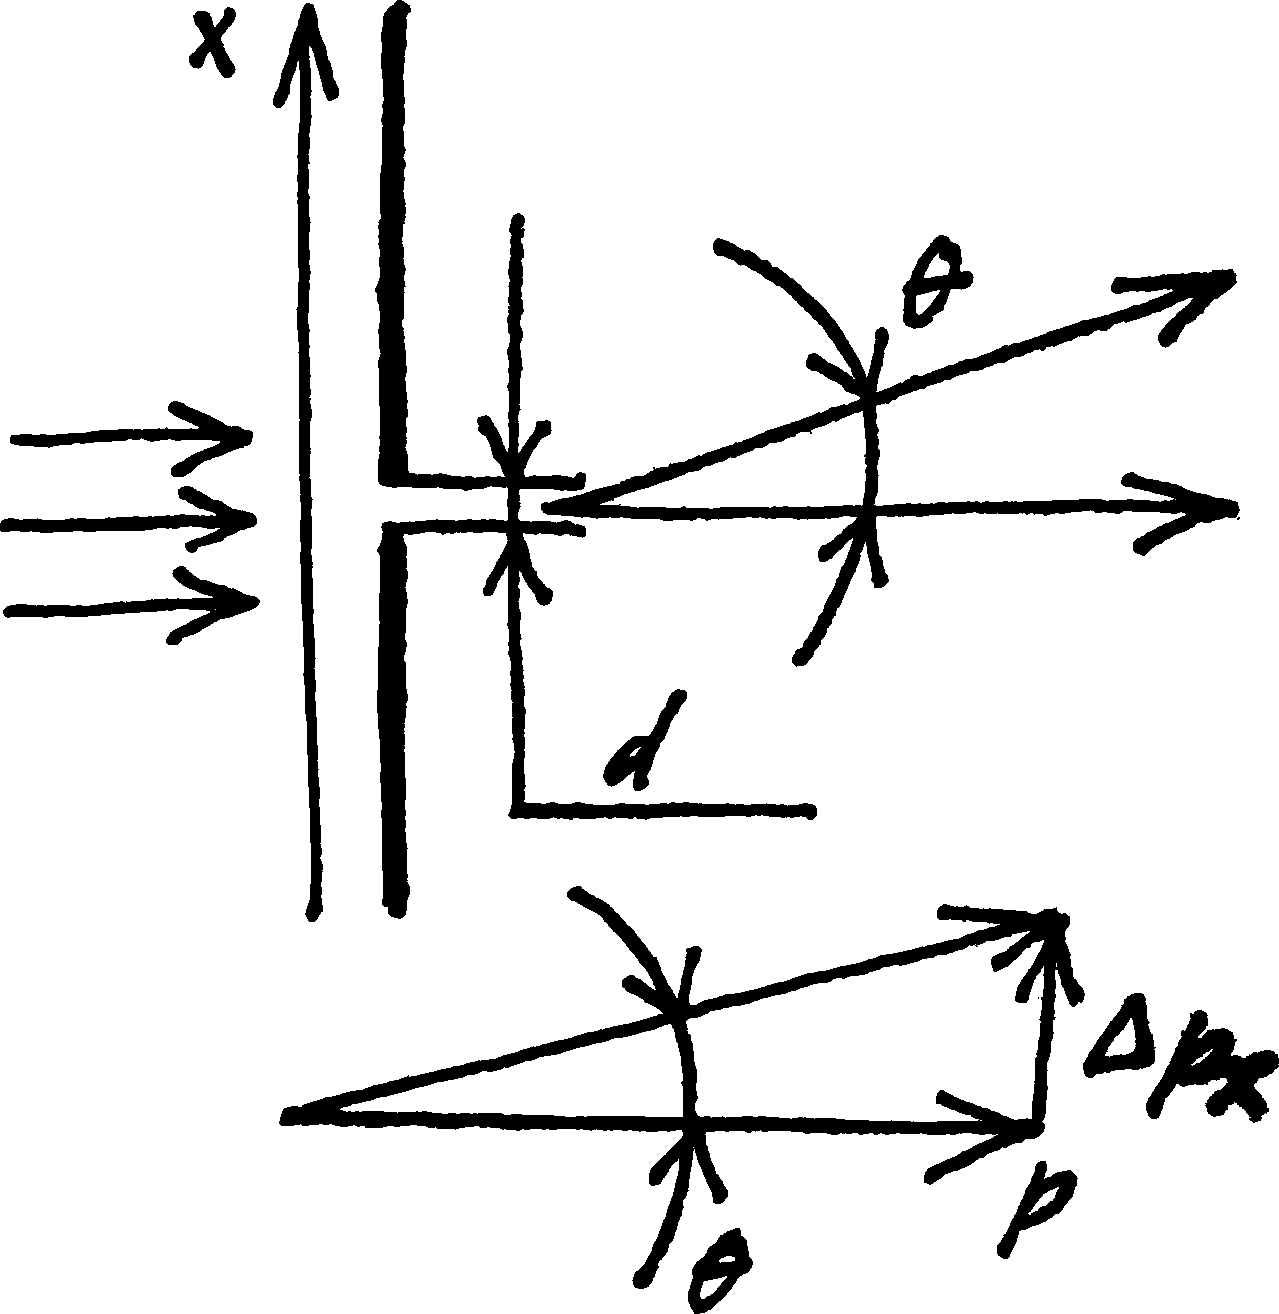
\includegraphics[width=\linewidth]{figures/fig-03-02.pdf}
\caption{Diffraction of microparticles from a slit.}
\label{fig-3.2}
\end{marginfigure}

Suppose (Figure \ref{fig-3.2}) a screen with a narrow slit is placed
in the path of a strictly parallel beam of certain microparticles with
momentum $p$. Let $d$ be the width of the slit along the $z$-axis (the
$x$-axis is perpendicular to the direction of the beam). Diffraction
takes place during the passage of microparticles through the slit. Let
$\theta$ be the angle between the initial direction and the direction of the
first (principal) diffraction peak. The classical wave theory gives
the following well-known relation for this angle:
\begin{equation*}%
\sin \theta = \frac{\lambda}{d}
\end{equation*}
Assuming angle $\theta$ to be sufficiently small, we can rewrite this
relation in the following form:
\begin{equation}%
 \theta \approx \frac{\lambda}{d}
\label{eq-3.5}
\end{equation}

If by $\lambda$ we now mean not the classical wavelength, but the length of the
de Broglie wave (i.e. the wave characteristic of the microparticle, we may
rewrite relation (\ref{eq-3.5}) in ``corpuscular language" by using the
expression (\ref{eq-2.11}): 
\begin{equation}%
\theta \approx  \frac{\hbar}{pd} 
\tag{3.5a}
\label{eq-3.5a}
\end{equation}
But how we are to understand the existence of the angle $\theta$ in
``corpuscular language''?  Obviously, it means that while passing
through the slit, the microparticle acquires a certain momentum
$\Delta p_{x}$ in the direction of the $x$-axis. It is easy to see that
$\Delta p_{x}\sim p \theta$. Substituting (\ref{eq-3.5a}) into this,
we get 
\begin{equation*}
\Delta p_{x} \approx  \frac{\hbar}{d} 
\end{equation*}
By considering the quantity $d$ as the uncertainty $\Delta x$ in the
$x$-coordinate of the microparticle passing through the slit, we get
\begin{equation*}
\Delta p_{x}\Delta x \approx \hbar, 
\end{equation*}
i.e. we arrive at the uncertainty relation (\ref{eq-3.3}). Thus the
attempt to determine in some way the coordinate of a microparticle in
a direction perpendicular to the direction of its motion leads to an
uncertainty in the momentum of the microparticle in that direction,
which also explains the phenomenon of diffraction observed in the
experiment.

In order \marginnote{Uncertainty Relations and the State of
  Microparticles. The Concept of a Complete Set of Physical
  Quantities}to describe the \emph{state} of a classical object it is
necessary to give a definite set of numbers - the coordinates and the
velocity components. In doing this other quantities, in particular,
energy, momentum and angular momentum of the object will also be
determined [see (\ref{eq-1.1})] The uncertainty relations show that
  this method of defining a state is not applicable to
  microparticles. Thus, for example, the existence of a definite
  projection of momentum in a given direction for a microparticle
  means that the position of the microparticle in this direction
  cannot be determined unambiguously: according to (\ref{eq-3.3}), the
  corresponding spatial coordinate is characterized by an infinitely
  large uncertainty. The electron in an atom has a definite energy;
  moreover its coordinates are characterized by an uncertainty of the
  order of the linear dimensions of the atom. This [according to
  (\ref{eq-3.3})] leads to an uncertainty in the projection of the momentum of
  the electron equal to the ratio of Planck's constant to the linear
  dimension of the atom.

  We now indicate the following situations, fundamental in quantum
  mechanics, which arise from the uncertainty relation: 
  \begin{enumerate}[label=(\alph*),leftmargin=1cm]
  \item various dynamic variables of a microparticle are combined in
    sets of simultaneously determined (simultaneously measurable)
    quantities, the so-called complete sets of quantities;
  \item various states of a microparticle are combined in groups of
    states corresponding to different complete sets of
    quantities.
\end{enumerate}
Each group contains the states of the microparticle in which the
values of the corresponding complete sets are known (it is customary
to say that every complete set has its own method of defining its
states).

We shall give examples of the complete sets employed for determining
the states of, say, an electron and a photon. Each of the sets
includes four quantities (because of this we say that a microparticle
like an electron or a photon has \emph{four degrees of freedom}). To
describe the states of an electron, the following sets are employed:
\begin{align}%
& x, \, y,  \, z,  \, \sigma \tag{3.6a} \label{eq-3.6a}\\
& p_{x}, \, p_{y}, \, p_{z},  \, \sigma \tag{3.6b} \label{eq-3.6b}\\
& E, \, l, \, m, \, \sigma \tag{3.6c} \label{eq-3.6c}
\end{align}

(remember that $l$, $m$, and $\sigma$ are orbital, magnetic and spin
quantum numbers, respectively). We emphasize that the coordinates and
the momentum components of a microparticle (in this case an electron)
fall in different complete sets of quantities; these two physical
quantities cannot be measured simultaneously. Hence the classical
relations (\ref{eq-1.2}) and (\ref{eq-1.3}) are not valid when going over to
microparticles, since each of these relations contains the coordinates
as well as the momentum.

The set (\ref{eq-3.6b}) is used, in particular, for a describing the states of
a freely moving electron. Moreover, the energy of the electron also
turns out to be definable\sidenote{ In contrast to relation
    (\ref{eq-1.2}), the classical relation $E = \frac{p^{2}}{2m}$ remains valid for a freely moving particle when going over to microparticles.}: 
\begin{equation*}
  E = \frac{( p_{x}^{2}+ p_{y}^{2} + p_{z}^{2})}{2m}
\end{equation*}

The set (\ref{eq-3.6c}) is usually employed for describing the states
of an electron in the atom. To describe the states of a photon, the
following sets arc most commonly employed:
\begin{align}%
& k_{x}, \, k_{y}, \, k_{z},  \, \alpha \tag{3.7a} \label{eq-3.7a}\\
& E, \, M^{2}, \, M_{z}, \, P \tag{3.7b} \label{eq-3.7b}
\end{align}

Here $k_{x}, \, k_{y}, \, k_{z}$ are the projections of the wave
vector of the radiation; $\alpha$ is the polarization of the photon;
$M^{2}$ and $M_{z}$ are the square of the momentum and the projection
of the momentum of the photon, respectively; $P$ is a quantum number
called the spatial parity. We notice that as soon as the projections
of the wave vector of radiation are determined, the projections of the
photon momentum are also known (recall that $\vec{p} = \hbar k$ ).
The \emph{polarization} of a photon may take two values corresponding
completely to the two independent polarizations of a classical wave
(thus, for example, one might talk about a photon having right
elliptical polarization). 

The \emph{spatial parity} is a characteristic property of a
microparticle; it may be considered as an integral of motion whose
conservation is a result of symmetry with respect to the operation of
reflection by a mirror. At a later stage (see Section \ref{sec-20}) we shall
discuss it in greater detail. Here, we only mention that parity can
assume one of the two values: +1 and -1.

The set (\ref{eq-3.7a}) is used for describing the states of photons
corresponding to plane classical waves, in this case the energy of the
photon is also defined (recall that $E = \hbar \omega = \hbar
ck$). The states described by the set (\ref{eq-3.7a}) are called $k
\alpha$-states. The set (\ref{eq-3.7b}) is employed for describing the
states of photons belonging to \emph{spherical} classical waves. We
note that just as a spherical wave may be represented as a
superposition of plane waves, the states of a photon described by the
set (\ref{eq-3.7b}) may be represented as a ``superposition" of states
described by the set (\ref{eq-3.7a}). The converse statement regarding
the representation of plane waves as a superposition of spherical
waves is also true. Here we have touched upon (for the present just
touched upon) one of the most important and delicate aspects of the
quantum-mechanical description of matter - the specific character of
the ``interrelations" between states of a microparticle described by
different complete sets. This specific character is reflected in the
most constructive principle of quantum mechanics - the \emph{principle
  of superposition of states}. The superposition of states will be
considered in detail in the second chapter; here we shall just
restrict ourselves to the above-mentioned remarks.

The \marginnote{The Uncertainty Relations and Quantum Transitions}
main contradiction regarding quantum transitions indicated in Section
\ref{sec-02} is essentially overcome by making use of the idea of
duality or, more precisely, the uncertainty relation
(\ref{eq-3.2}). Let us consider transition of an electron in an atom
from level $E_{1}$ to level $E_{2}$ by absorbing a photon of energy
$\hbar \omega = E_{2} - E_{1}$. We recall that the contradiction in
transition was connected with the question whether the absorption of
the photon precedes the transition of the electron or vice versa. It
is easy to see that this question simply loses its meaning now. In
fact, if we have a bound electron with energies $E_{1}$ and $E_{2}$
before and after interaction with radiation, respectively, then during
the interaction we have one quantum-mechanical system including both
the electron and the radiation. This system exists for a definite time
(while the interaction with the radiation takes place) and, according
to (\ref{eq-3.2}), cannot have any definite energy. Hence it is
meaningless to find out precisely what takes place in such a
system. Strictly speaking, during the interaction of the electron with
the photon there is no electron and no photon, but a single entity
which must be treated as such, without going into details. This
example shows that in quantum mechanics a physical process cannot be
infinitely detailed in time. The question ``what follows what"? cannot
always be posed in the case of microphenomena.\sidenote[][-1.5cm]{The anomaly of
  quantum transition is completely removed by considering the
  principle of superposition of states (see Section \ref{sec-10}).}

\begin{fullwidth}
  \setlength{\leftskip}{3cm} \textsf{\small The uncertainty relation
    (\ref{eq-3.2}) allows us to introduce and employ a very important
    concept in quantum theory, the so-called \emph{virtual
      transitions}, for explaining quantum transitions. We shall give
    here a simplified treatment of virtual transitions, but we shall
    give a detailed explanation later in Section
    \ref{sec-06}. According to relation (\ref{eq-3.2}), an electron
    may go over from level $E_{1}$ to $E_{2}$ without getting any
    energy from outside; what is important is that it should quickly
    return to its initial level $E_{1}$. Such a ``journey'' ($E_{1}
    \to E_{2} \to E_{1}$) is possible if its duration $\Delta t$ is
    such that the inequality $\nicefrac{\hbar}{\Delta t} \gg (E_{2} -
    E_{1}$) is satisfied, because in this case the uncertainty in the
    energy of the electron is greater than the difference in the
    energies of the levels under consideration. Hence it is clear that
    the statement ``the electron occupies level $E_{1}$'' may be
    understood quite' specifically-as incessant ``transition'' of the
    electron from the given state to others with an inevitable return
    every time to the starting level $E_{1}$. Such transitions cannot
    he observed experimentally, and are called virtual transitions in
    contrast to the normal (real) transitions. During interaction of
    an electron undergoing virtual transitions with radiation, the
    electron is liable to change its ``residence''. For example, it
    might now occupy level $E_{2}$ and will in future perform virtual
    transitions not from level $E_{1}$, but from level $E_{2}$. If
    such a thing happens, the electron is said to have absorbed a
    photon of energy $\hbar \omega = E_{2} - E_{1}$, and undergone a
    transition from level $E_{1}$ to $E_{2}$. Virtual transitions
    don't require any expenditure of energy from outside while a real
    transition cannot occur without expenditure of energy - the energy
    of the photons absorbed (or emitted) by electrons during
    interaction with radiation.}

    \textsf{\small To explain the difference between real and virtual transitions,
    we note that a real transition from a level $E_{1}$ to another level
    $E_{2}$ and back may be broken up into two successive events in time
    (in between the electron may be experimentally registered in the
    intermediate state $E_{2}$). However, the virtual transition from
    level $E_{1}$ to $E_{2}$ and back cannot be broken up into two events in
    time - both parts of the transition must be considered as a single,
    indivisible process in time.}
\end{fullwidth}
\vspace{5pt}
\setlength{\leftskip}{0pt}

The \marginnote{Uncertainty Relation ``Number of Photons-Phase''}
uncertainty relations used in quantum theory are by no means exhausted
by relations (\ref{eq-3.2})-(\ref{eq-3.4}). As an example of one more
such relation we consider the uncertainty relations for the number
of photons and the phase of the wave.

Let there be a monochromatic radiation of frequency $\omega$. On one hand,
it may be considered as a collective of photons each having energy
$\hbar \omega$; on the other hand, we might treat it as a classical
electromagnetic wave. Let $N$ be the number of photons in the volume
under consideration and let $\Phi = \omega t$ be the phase of the classical
wave. The corpuscular characteristic of the radiation (number of
photons $N$) and its wave characteristic (phase $\Phi$ cannot have definite
values simultaneously; there exists the uncertainty relation 
\addtocounter{equation}{2}
\begin{equation}%
\Delta N \Delta \Phi \ge 1 
\label{eq-3.8} 
\end{equation}

In order to arrive at relation (\ref{eq-3.8}), we start from the
uncertainty relation for energy and time. We recall that for measuring
the energy of a quantum object with an accuracy $\Delta E$ we must
spend time $\Delta t \ge \dfrac{\hbar}{\Delta E}$. If we take the
collective of photons as the quantum object, we get
\begin{equation*}%
\Delta E = \hbar \omega \Delta N  
\end{equation*}
where $\Delta N$ is the uncertainty in the number of photons. During
the time $\Delta t$ necessary for measurement of the energy of the
object with an accuracy $\hbar \omega \Delta N$, the phase $\Phi$
changes by $\Delta \Phi = \omega \Delta t$. Substituting into this the
relation $\Delta t \ge \dfrac{\hbar}{\hbar \omega \Delta N}$, we
find
\begin{equation*}%
\Delta \Phi \ge \frac{1}{\Delta N}  
\end{equation*}
\marginnote[-1cm]{Q.E.D.}

Relation (\ref{eq-3.8}) reflects the dialectically contradictory unity
of corpuscular and wave properties of radiation. The uncertainty
$\Delta \Phi$ is small when the wave properties of radiation are
clearly exhibited; in this case the density of photons is high ($N$ is
large) and so is the uncertainty $\Delta N$. On the other hand, the
uncertainty $\Delta N$ is small when there are a few photons in the
aggregate. In this case the corpuscular properties of radiation are
clearly exhibited and therefore the uncertainty $\Delta \Phi$ is large.

\section{Some Results Ensuing from the Uncertainty Relations}
\label{sec-04}
The \marginnote{Evaluation of Energy of Ground State of Hydrogen Atom}
uncertainty relations serve as very useful working tools of quantum
theory since they permit one to obtain important results, by fairly
simple means. 

As an example, we consider the \emph{hydrogen atom} in its ground
state, We make use of the well-known classical expression for energy
of a charged particle moving in a Coulomb field: 
\begin{equation}
E = \frac{p^{2}}{2m} - \frac{e^{2}}{r}
\label{eq-4.1}
\end{equation}
where $m$ and $e$ are the mass and charge of the electron,
respectively. In order to use the classical expression (\ref{eq-4.1}) in the
quantum theory, we consider the quantities $p$ and $r$ occurring in it as
uncertainties in momentum and coordinates of the electron,
respectively. According to relation (\ref{eq-3.3}), these quantities are
connected with each other. We assume  $pr \approx \hbar$, or, simply, 
\begin{equation}%
pr = \hbar
\label{eq-4.2} 
\end{equation}
Eliminating the quantity $r$ from (\ref{eq-4.1}) by using (\ref{eq-4.2}), we get
\begin{equation}%
E(p) = \frac{p^{2}}{2m} - \frac{e^{2}p}{\hbar}
\label{eq-4.3} 
\end{equation}
It is easy to see that the function $E(p)$ has a minimum for a certain
value $p= p_{1}$. We denote it as $E_{1}$. The quantity $E_{1}$ may be
considered as the energy of the ground state of the hydrogen atom
while the quantity $r_{1} = \dfrac{\hbar}{p_{1}}$ is the estimate of
the linear dimensions of the atom (in Bohr's theory this is the radius
of the first orbit). By equating the derivative $\dfrac{d}{dp} E (p)$
to zero, we find $p_{1} = \dfrac{me^{2}}{\hbar}$. This at once gives
the required evaluations (cf. (\ref{eq-2.6}) and (\ref{eq-2.7})]: 
\begin{equation}%
\left.
\begin{split}
r_{1} & = \frac{\hbar^{2}}{me^{2}} \\
E1 &= - \frac{me^{4}}{2 \hbar^{2}} 
\end{split}
\right \}
\label{eq-4.4}
\end{equation}
The values given by (\ref{eq-4.4}) fully coincide with the results of
the rigorous theory.\sidenote{In the rigorous theory the quantity
  $r_{1}$ is a characteristic for the ground state of the hydrogen
  atom and denotes the distance from the nucleus at which an electron
  is most likely to be observed (see expression (\ref{eq-5.4})).} Of
course such a complete coincidence must be considered to some extent
as an accidental success. Only the order of the quantities should be
taken seriously here. We emphasize that this order can be evaluated
quite simply as follows: it is sufficient first to simply replace the
precise values of the dynamic variables in expression (\ref{eq-4.1})
by quantities which characterize the degree of ``blurring'' of these
variables, i.e. by their uncertainties, and then use the
quantum-mechanical relations connecting the said uncertainties.

We \marginnote{Estimate of the Energy of Zero-point Oscillations of an
  Oscillator} shall proceed exactly in the same way as in the preceding
example. The energy of a classical one-dimensional harmonic
oscillator is given by the expression
\begin{equation}%
E = \frac{p^{2}_{x}}{2m} + \frac{m \omega^{2}x^{2}}{2}
\label{eq-4.5} 
\end{equation}
Treating $p_{x}$ and $x$ as uncertainties in the momentum and coordinate of
the oscillating microparticle and using the equality $px \cdot x = \hbar$ as the
uncertainty relation, we get from (\ref{eq-4.5}) 
\begin{equation}%
E (p_{x}) = \frac{p^{2}_{x}}{2m} + \frac{m \omega^{2}\hbar^{2}}{2p_{x}^{2}}
\label{eq-4.6} 
\end{equation}
By equating the derivative $\dfrac{d}{dp} E (p_{x})$ to zero we find
the value of $p_{0} = \pm \sqrt{m \hbar \omega }$ for which the
function $E(p_{x})$ assumes its minimum value. It is easy to see that
this value is 
\begin{equation}%
E_{0} = E(p_{0}) = \hbar \omega
\label{eq-4.7} 
\end{equation}
This result is quite interesting. It shows that in quantum mechanics
the energy of an oscillator cannot vanish; its minimum value is of the
order of $\hbar \omega$. This is the energy of what is called the zero-point
oscillation. We note that the estimate (\ref{eq-4.7}) differs from the exact
expression for the energy of the zero-point oscillation just by a
factor of $\dfrac{1}{2}$ (exact value $E_{0} = \dfrac{1}{2} \hbar
\omega$).  

By taking the zero-point oscillations into account, one may arrive at
the following interesting conclusion: the energy of the oscillatory
motion of atoms in a crystal does not vanish even at absolute zero.
The zero-point oscillations illustrate a basically general
circumstance: it is impossible to find a microparticle at the ``bottom
of the potential well'', or, in other words ``a microparticle cannot
fall to the bottom of the potential well.'' This conclusion does not
depend on the form of the potential well, since it is a direct
consequence of the uncertainty relation: ``falling to the bottom of the
well'' is connected with the vanishing of momentum and hence the
uncertainty in the momentum of the microparticle. In this case, the
uncertainty in the coordinate becomes so large that there is a direct
contradiction with the very fact that the microparticle is in a
potential well.

The \marginnote{Evaluation of the ``Blurring'' of the Optical
  Absorption Band Edge in the Franz-Keldysh Effect}essence of the
effect, investigated in 1958 by Keldysh, and independently by Franz,
lies in the following: in a uniform external electric field, the
minimum of the electron energy in the conduction band of
semiconductors shifts downwards on the energy scale, leading to a
``blurring'' of the edge of the fundamental optical absorption band
(as a result the absorption of the photons with energies lower than
the forbidden band width becomes possible) [\cite{22}]. The value of the
shift of electronic states characterizing the indicated ``blurring'' may
be obtained in the same way as the preceding evaluations were made. We
make use of the classical expression for the energy of a charged
particle in the electric field of intensity $\Ea$: 
\begin{equation}%
E = \frac{p_{x}^{2}}{2m}-\Ea ex 
\label{eq-4.8} 
\end{equation}

Here $m$ is the effective mass of the electron in the conduction
band. Treating $p_{x}$ and $x$ as uncertainties in the momentum and
coordinate of the electron and using the equality $p_{x} \cdot x = \hbar$. as the
uncertainty relation, we get from (\ref{eq-4.8}) 
\begin{equation}%
E(p_{x}) = \frac{p_{x}^{2}}{2m}-\frac{\Ea e \hbar}{p_{x}} 
\label{eq-4.9} 
\end{equation}

Next, as usual we equate the derivative $\dfrac{d}{dp_{x}} E (p_{x})$
to zero and obtain the value $p_{0}== - \sqrt[3]{\Ea e \hbar m}$ for
which the function $E(p_{x})$ assumes its minimum value:
\begin{equation}%
\begin{split}
E_{0} & = \frac{3}{2} \sqrt[3]{\dfrac{(\Ea e \hbar)^{2}}{m}} \\
& \approx \sqrt[3]{\dfrac{(\Ea e \hbar)^{2}}{m}} 
\end{split}
\label{eq-4.10}
\end{equation}
Expression (\ref{eq-4.10}) gives an estimate of the extent of the
``blurring'' of the edge of the fundamental optical absorption band in
the Franz-Keldysh effect.

While postulating the stationary states, Bohr's theory \marginnote{Why
  does not the Electron Fall into the Nucleus?}did not explain why,
after all, the electron, moving under acceleration, does not radiate
and fall into the nucleus as a result of this. Relation (\ref{eq-3.3})
explains this fact. The falling of an electron into a nucleus would
obviously mean a considerable reduction in the uncertainty of its
coordinate. Before the hypothetical falling into the nucleus, the
electron is localized within the limits of the atom, i.e. in a region
of space with linear dimensions $\dfrac{\hbar^{2}}{me^{2}} \approx
  \SI{d-8}{\centi\meter}$ [see (\ref{eq-4.4})], whereas after falling
  into the nucleus it would be localized in a region with linear
  dimensions less than \SI{d-12}{\centi\meter}. According to
  (\ref{eq-3.3}) a stronger localization of a microparticle in space
  is linked with a ``blurring'' of its momentum. Hence upon falling into
  the nucleus, the mean value of the momentum of the electron must
  increase, which requires an expenditure of energy. Thus it turns
  out that effort has to be made not to ``hold'' the electron from
  falling into the nucleus, but on the contrary to ``force'' the electron to be
  localized within the nucleus. 

  In the example of the zero-point oscillations it was pointed out
  that the microparticle in a potential well always possesses a
  non-zero minimum energy $E_{0}$. The magnitude of $E_{0}$ depends, in
  particular, on the spatial dimensions of the well (or on its width
  $a$, which determines the extent of localization of the microparticle
  in space). By taking into account the uncertainty relation, it is
  easy to see that 
  \begin{equation}%
    E_{0} \approx \frac{\hbar^{2}}{ma^{2}}
    \label{eq-4.11}
  \end{equation}
  
  If $a$ decreases, $E_{0}$ increases. For sufficiently small $a$, the
  energy $E_{0}$ may become greater than the depth of the potential
  well. It is obvious that such a well will not hold the microparticle
  at all.  

  The falling of an electron into the nucleus corresponds to a
  decrease in the width of the potential well from
  \SIrange{d-8}{d-12}{\centi\meter} (and even lower). According to
  (\ref{eq-4.11}) the minimum energy $E_{0}$ should increase in this
  case from \SIrange{10}{d9}{\electronvolt} (and higher). As a result
  the minimum energy of the electron turns out to be a few orders
  higher than the binding energy of a nucleon in the atomic nucleus
  (the latter being not greater than \SI{d7}{\electronvolt}). This
  means that the electron cannot ever be present in the nuclear
  potential well and hence it can by any means be compelled to be
  localized within the nucleus, not even by force. This not only
  eliminates the problem of ``an electron falling into the nucleus''
  but also solves another fundamental question: the \emph{electron is not
  one of the constituents of the atomic nucleus}.

In order \marginnote{On the ``Trajectory'' of Microparticles}to draw
the trajectory of a particle, it is necessary, strict]y speaking, to
know the coordinate and momentum of the particle at every moment of
time (in fact, in order to depict the dependence $x (t)$, it is
necessary to know, for every $t$, the values $x$ and
$\dfrac{dx}{dt}$). Since,according to the uncertainty relation
(\ref{eq-3.3}), a microparticle cannot simultaneously possess a
defInite coordinate and a definite projection of the momentum, one can
draw the conclusion that the concept of trajectory in case of
microparticle, strictly speaking, is not applicable.

  The rejection of the trajectory concept is connected with the
  existence of wave properties in microparticles, which do not permit
  one to consider microparticles as classical corpuscles. The movement
  of a microparticle along the $x$-axis cannot be associated with the
  differentiable function $x (t)$ which is so widely used when
  considering the mechanics of classical objects. From a known value
  of $x$ of the microparticle at a certain time $t$, it is impossible to
  predict the value of its coordinate at the time $t + dt$.

  As applied to Bohr's theory, this means a rejection of the very
  concept of ``the orbit of an electron in an atom''. One may speak
  about the localization of the electron within the atom as a whole;
  the orbit requires a much greater spatial localization. Turning to
  the problem of ``the electron falling into the nucleus'' discussed
  above, we can understand the consequence to which such a
  localization leads. The planetary model of the atom thus turns out
  to be just an intermediate step in development of our concept of the
  atom. Much later, in the fifties, Bohr himself amusingly recalled
  how after one of his lectures a student came up and asked him ``Were
  there really idiots who thought that the electron revolves in an
  orbit?''

\begin{fullwidth}
  \setlength{\leftskip}{3cm} \textsf{\small We note that with the
    rejection of the idea of orbits of the electron in an atom the
    contradiction regarding the problems of the instantaneous jump of
    the electron from one orbit into another, discussed in Section
    \ref{sec-02}, is automatically eliminated.}
\end{fullwidth}
\vspace{5pt}
\setlength{\leftskip}{0pt}


There are situations, however, in which one can make use of the idea
of ``the trajectory of a microparticle'' As an example we consider the
motion of electrons in the kinescope of a television set. The momentum
of the electron along the axis of the tube is $p = \sqrt{2meU}$, where
$U$ is the accelerating voltage. The formation of the electron beam
means a definite localization of the coordinate in the transverse
direction. The degree of this localization is characterized by the
diameter $d$ of the beam. According to (\ref{eq-3.3}), there must be
an uncertainty in the electron momentum in a direction perpendicular
to the axis of the beam: $\Delta p \approx \dfrac{\hbar}{d}$. As a
result of this uncertainty, the electron may deviate from the axis of
the beam within an angle $\Delta \theta \approx \dfrac{\Delta p}{p}
\approx \dfrac{\hbar}{pd}$. Let $L$ be the path length of the electron
in the kinescope. Then the uncertainty in the position of the point of
impingement of an electron on the screen will be characterized by the
quantity $\Delta x \approx L \Delta \theta \approx \dfrac{L
  \hbar}{pd}$. Assuming $U = \SI{20}{\kV}, d = \SI{d-3}{\cm}, L =
\SI{d2}{\cm}$, we get $\Delta x \approx \SI{d-5}{\cm}$. In this way,
the blurring of the point of impingement due to the uncertainty
relation is considerably less than the diameter of the beam. It is
clear that in such cases the motion of the electron may be treated
classically.

  

Suppose \marginnote{The Possibility of a Microparticie Sub-Barrier
  Passage (Tunneling Effect)}we have a potential barrier whose height
$U$ is greater than the energy of the particle (Figure
\ref{fig-4.1}). We ask the question: can a particle, situated
somewhere to the left of the barrier, appear after some time to the
right of it, without getting any energy from outside? Classical
mechanics gives a negative answer -- a classical corpuscle cannot pass
through the barrier. If this were to happen, then the total energy of
the particle, say, at the point A in Fig. 4.1 would be less than its
potential energy, which is physically absurd.

\begin{marginfigure}%[1cm]%
\centering
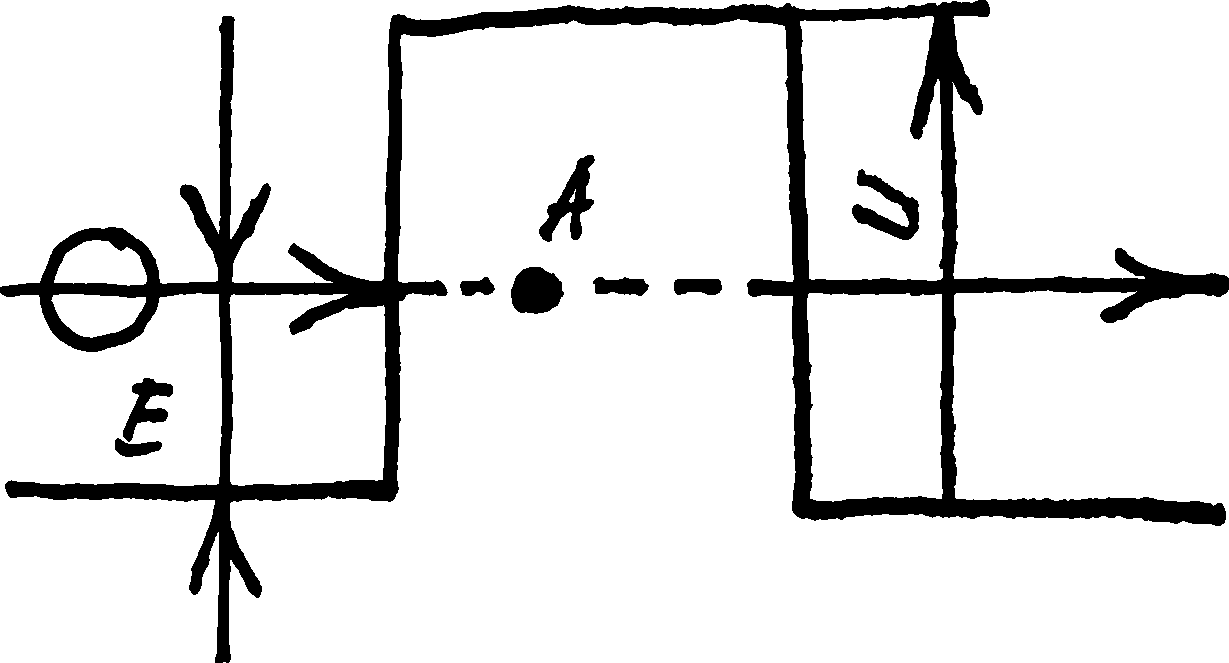
\includegraphics[width=\linewidth]{figures/fig-04-01.pdf}
\caption{A microparticle tunneling through a barrier.}
\label{fig-4.1}
\end{marginfigure}

Does this ban apply to microparticles as well? It can be shown that it
does not -- it is removed by relation (\ref{eq-3.2}). Let the
microparticle move from infinity to the right and encounter the
potential barrier. Until this encounter it was in a state of free
motion for an infinitely long time and hence its energy had a definite
value. But now the microparticle interacts with the barrier, or, more
precisely, with the objects which caused the appearance of the
barrier. Suppose the interaction lasts for a time $\Delta
t$. According to (\ref{eq-3.2}), the energy of the microparticle in a
state of interaction with the barrier is no longer definite but is
characterized by the uncertainty $\Delta E \ge \dfrac{\hbar}{\Delta
  t}$. If this uncertainty is of the order of the height $U$ of the
barrier, the latter stops being an unsurmountable obstacle for the
microparticle. Thus the microparticle may pass through the potential
barrier. This specific quantum effect is called the \emph{tunneling
  effect}. It explains, in particular, the $\alpha$-decay of atomic
nuclei. It should be noted that when considering the tunneling effect,
the motion of the microparticle cannot be represented by the dotted
line in Figure \ref{fig-4.1}. The dotted line corresponds to the classical
trajectory, while a microparticle does not have a trajectory. Hence
there is no point in trying to ``accuse'' the microparticle of having
been ``under the potential barrier'' at some moment of time.

\begin{fullwidth}
  \setlength{\leftskip}{3cm} \textsf{\small It has been noted above
    that the energy of a freely moving micro particle is not
    quantized. This may be easily shown by making use of the tunneling
    effect. Suppose a microparticle is located in a potential well
    shown in Figure \ref{fig-4.2}. On account of the tunneling effect
    the mlcroparticle may of its own accord leave the potential
    well. Consequently, the time for which it stays in the well is not
    infinite. If we denote this time as $\Delta t$, it follows from
    (\ref{eq-3.2}) that the energy of the microparticle must have an
    uncertainty of the order $\dfrac{\hbar}{\Delta t}$. We reduce the
    width $b$ of the potential barrier (dotted line in Figure
    \ref{fig-4.2}). It is clear that as a result the magnitude of
    $\Delta t$ will decrease, since the probability of the
    rnicroparticle leaving the well will increase. With a decrease in
    $\Delta t$, the uncertainty in the energy of the microparticle,
    $\dfrac{\hbar }{\Delta t}$, will increase. This may be considered
    as a larger blurring (further broadening) of the energy levels of
    the rnicroparticle in the well. In the limiting case of zero
    thickness of the barrier, the value of $\Delta t$ vanishes, the
    microparticle becomes a freely moving particle, and the energy
    levels broaden up indefinitely, actually transforming into a
    continuous energy spectrum.}
\end{fullwidth}
\vspace{5pt}
\setlength{\leftskip}{0pt}


\begin{marginfigure}[5cm]%
\centering
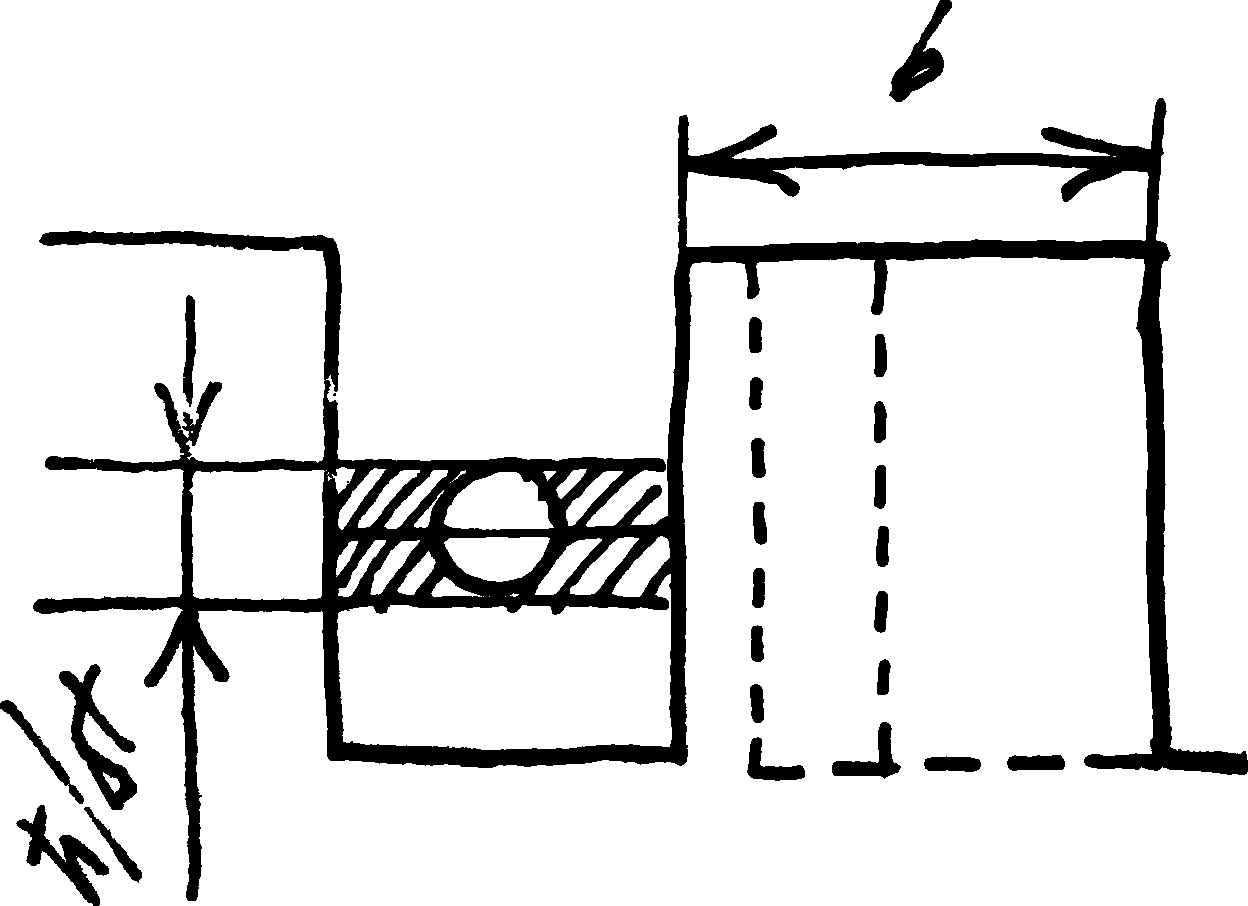
\includegraphics[width=\linewidth]{figures/fig-04-02.pdf}
\caption{A microparticle tunneling through a barrier.}
\label{fig-4.2}
\end{marginfigure}
\section{Impossibility of Classical Representation of a Microparticle}
\label{sec-05}
The process \marginnote[.5cm]{A Microparticle Is not a Classical Corpuscle}
of ``breaking up'' of objects surrounding us into smaller and smaller
``fractions'' leads to microparticles. Therefore it is but natural to
associate microparticles first of all with corpuscles. This is also
supported by the fact that a microparticle is characterized by a
definite rest mass and a definite charge. For instance, it is
meaningless to speak of a half-electron having half the mass and half
the electric charge of a whole electron. The very terms
``microparticle'' and ``elementary particle'' reflect the notion of the
microparticle as being some particle (corpuscle).

However, as follows from the preceding discussion, a microparticle is considerably different from a classical corpuscle. Firstly it does not have a trajectory which is an essential attribute of a classical corpuscle. The use of such corpuscular characteristics as coordinate, momentum, angular momentum, energy when considering microparticles is restricted to the framework of the uncertainty relations. Interconversion of microparticles, spontaneous decays, the existence of an indestructible intrinsic moment (spin) and the ability to pass through potential
barriers indicate that microparticles are quite dissimilar to
classical corpuscles. 

Wave concepts are radically different from corpuscular concepts. Hence
it is not surprising that the striking contrast between classical
corpuscles and microparticle is explained by the existence of wave
properties in the latter. Moreover, it is the wave properties which
account for the uncertainty relations and all the consequences
resulting from them. In this respect, the following remark by de
Broglie [23] is worth noting: ``for a century, the corpuscular method
of analysis in optics was too much neglected in comparison with the
wave method. Hasn't the converse been the case in the theory of
matter?  Haven't we thought too much of the ``particle'' picture and
neglected the wave aspect far too much?'' The question raised by de
Broglie is fully justified. However, an excessive exaggeration of the
wave aspect while considering microparticles should be avoided. We
must remember that while on one hand a microparticle is not a
classical corpuscle, it is similarly, on the other hand, not a
classical wave.

The \marginnote{Microparticle Is not a Classical Wave} analysis of one
mistake which is committed quite often even these days when
considering a simplified account of quantum mechanics is quite
instructive. We shall demonstrate this mistake through two examples.

It \marginnote{Example 1}is contended that the wave properties of an
electron permit one to derive the conditions for the quantization of
momentum which are postulated in Bohr's theory. The ``derivation'' is
done in the following way Let $2 \pi r_{n}$ be the perimeter of the
$n$-th Bohr's orbit. In this orbit, an electron moves with de
Broglie's wavelength $\lambda_{n} = \dfrac{2 \pi \hbar }{p_{n}}$. The
basic assumption lies in the fact that the perimeter of the orbit
should contain $n$ wavelengths $\lambda_{n}$ of the
electron. Consequently, $2 \pi r_{n} = n \lambda_{n}$. This at once
gives the desired condition for quantization of momentum:
\begin{equation}%
p_{n}r_{n} = n \hbar 
\label{eq-5.1} 
\end{equation}
It is \marginnote{Example 2}stated that the wave properties of an
electron permit a very simple derivation of the formula for the energy
levels in a potential well, if we assume that a definite number of de
Broglie half-waves are confined in the potential well (in analogy with
the number of half-waves contained in the length of a string fixed at
both ends) corresponding to different stationary states. Designating
the width of the one-dimensional potential well by $a$, we write $a =
\dfrac{n \lambda_{n}}{2}$, from which we get the desired result:
\begin{equation}%
E_{n} = \frac{n^{2} \pi^{2} \hbar^{2}}{2 m a^{2}}
\label{eq-5.2} 
\end{equation}
Both these final results [(\ref{eq-5.1}) as well as (\ref{eq-5.2})]
are correct; they are the same as the result deduced from strict
theory. However, the ``derivation'' of these formulas must be
considered to be unsound. In both cases in fact the same fundamental
mistake has been committed: they are based on the wrong assumption
that the electron in a potential well has a definite de Broglie
wavelength, or, in other words, a definite momentum. However,
according to (\ref{eq-3.3}), the momentum of a microparticle in a
bound state is characterized by the uncertainty $\Delta p \ge
\dfrac{\hbar}{a}$. Since in the above examples $p \approx
\dfrac{\hbar}{\lambda} \approx \dfrac{\hbar}{a}$, it follows that the
momentum is of the same order of magnitude as the uncertainty in
momentum given by relation (\ref{eq-3.3}). It is clear that in such
cases one cannot speak about any value of the electron momentum (and
correspondingly of its de Broglie wavelength) even
approximately.\sidenote{ This question is considered in greater detail
  in Section \ref{sec-23} of this book. See also work by de Broglie. \citep{debroglie-1930}}  These
examples demonstrate an obvious exaggeration of the wave aspect. The
identification of an electron in a potential well with a classical
wave inside a ``resonator'' is incorrect. The picture of an electron
wave in a ``resonator'' is the same kind of simplification as the
picture of an electron-ball moving in a classical orbit. We shall
return again to the question of waves in quantum mechanics; however,
it is useful to emphasize at this stage that by the term ``de Broglie
wave'' we do not conceal any sort of classical wave. It is just a
reflection in our imagination of the fact that microparticles
possess wave properties.

If \marginnote{ Attempts to Represent a Microparticle as a Symbiosis
  of a Corpuscle and a Wave} a microparticle is neither a corpuscle
nor a wave, then may he it is some kind of a symbiosis of a corpuscle
and a wave? Several attempts were made to model such a symbiosis and
thus also to visually demonstrate the wave-particle duality. One such
attempt represents a microparticle as a formation, limited in space
and in time. This may be the wave packet mentioned in Section
\ref{sec-03}. This may also be just a ``scarp'' of a wave, often called
a wave train. Another attempt uses a model of a pilot-wave, according
to which a microparticle is some sort of a ``compound'' of a corpuscular
``core'' with a certain wave which controls the motion of the core.

\begin{fullwidth}
  \setlength{\leftskip}{3cm} \textsf{\small One of the versions of the
    pilot wave model is considered by D. Baum in his book
    \cite[-1.5cm]{bohm-1957}:} \textit{\small We first postulate that
    connected with each of the ``fundamental'' particles of physics
    (e.g. an electron) is a body existing in a small region of space
    \ldots \, in most applications at the atomic level the body can be
    approximated as a mathematical point \ldots \, The next step is to
    assume that associated with this body there is a wave without
    which the body is never found. This wave will be assumed to be an
    oscillation in a new kind of field, which is represented
    mathematically by the $\psi$-field of Schr\"odinger somewhat like
    the gravitational and the electromagnetic, but having some new
    characteristics of its own \ldots }

  \textit{\small We now assume that the $\psi$-field and the ``body''
    are interconnected in the sense that the $\psi$-field exerts a new
    kind of ``quantum-mechanical'' force on the body, the force is
    such as to produce a tendency to pull the body into regions where
    $I\psi I$ is largest. }

  \textit{\small If the above tendency were all that were present, the
    body would eventually find itself at the place where the
    $\psi$-field had the highest intensity. We now further assume that
    this tendency is resisted by random motions undergone by the body,
    motions which are analogous to the Brownian movement. They could,
    for example, come from random fluctuations in the $\psi$-field
    itself.}

  \textit{\small Once admitting the existence of these fluctuations,
    we then see that they will produce a tendency for the body to
    wander in a more or less random way over the whole space
    accessible to it. But this tendency is opposed by the ``quantum
    force'' which pulls the body into the places where the $\psi$-field is
    most intense. The net result will be to produce a mean
    distribution in a statistical ensemble of bodies, which favours
    the regions, where the $\psi$-field is most intense \ldots}

  \textsf{\small Figure \ref{fig-5.1} illustrates Hie given model as
    applied to the passage of a microparticle through the screen with
    slits: the $\psi$-wave is diffracted on both the slits, while the
    ``body'' passes through one slit and is registered on the screen
    in accordance with the result of the interference of $\psi$-waves.
  }
\begin{marginfigure}[6.5cm]%
\centering
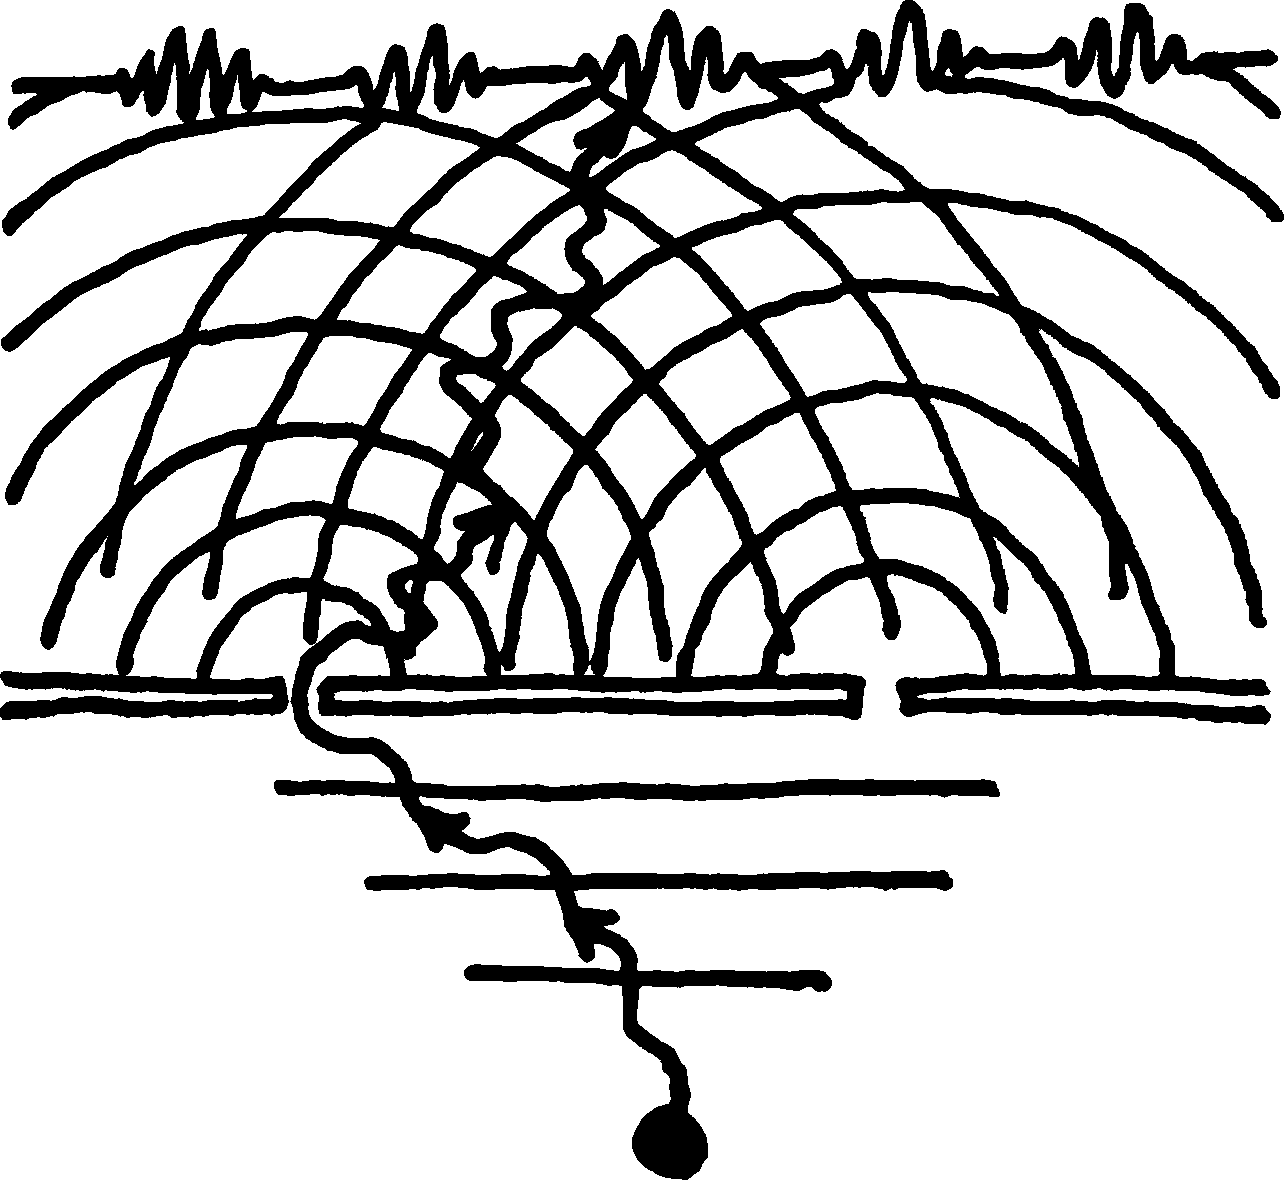
\includegraphics[width=\linewidth]{figures/fig-05-01.pdf}
\caption{Bohm's pilot wave model.}
\label{fig-5.1}
\end{marginfigure}



\end{fullwidth}
\vspace{5pt}
\setlength{\leftskip}{0pt}

It is not denied that such models could appear attractive at first
glance if only because of their intuitive appeal. It must be
emphasized at once, however, that all these models are baseless. We
shall not explain at this stage the reasons for worthlessness of the
pilot-wave model considered above, but shall just mention that it is
cumbersome since it uses artificial notions such as the $\psi$-field which
is ``to some extent similar to gravitational end electromagnetic
fields'', or the ``quantum force'' which reflects the interaction of
certain ``object'' with the $\psi$-field. The reader will later realize that
the worthlessness of such models is not because of some specific
feature, but because of deep fundamental reasons. He will understand
that any attempt at a literal interpretation of the wave-particle
duality, any attempt to model a symbiosis of corpuscle and a wave,
should be considered fruitless from the very start. A microparticle
is not a symbiosis of a corpuscle and a wave.

At \marginnote{How to Understand the Wave-Particle Duality}present the
wave-particle duality is considered as the potential ability of a
microparficle to exhibit its different properties depending on
external conditions, in particular, on the conditions of
observation. As Fock wrote: 
\begin{quote}
  Thus under certain conditions an atomic object may exhibit wave
  properties and under other conditions corpuscular properties;
  conditions are also possible when both kinds of properties appear
  simultaneously but not sharply. We can state that it is potentially
  possible for an atomic object to manifest itself either as a wave or
  as a particle or in an intermediate fashion, according to the
  external condition prevailing. It is just this potential possibility
  of exhibiting various properties inherent in an atomic object that
  constitutes the wave-corpuscular duality. Any other, more literal
  meaning attached to this duality, such as a wave-particle model of
  any kind, is incorrect.\cite{fock-1957}  
\end{quote}

Let us consider a simple example. Let a beam of electrons pass through
a screen with slits and then hit a detector screen. While passing
through the slits, the electrons realize their wave properties which
leads to a distribution for electrons beyond the slit characteristic
of interference. When impinging on the detector screen, the electrons
exhibit their corpuscular properties -- each of them is registered at
a certain point on the screen. It may be said that the electron passes
through the slit as a ``wave'', and is registered on the detector
screen as a ``particle'' In this connection, it is sometimes said that
a microparticle is a wave under some circumstances, and a
microparticle is a particle under other circumstances. Such a
treatment of wave-particle duality is incorrect. Whatever the
conditions, a microparticle is neither a wave, nor a particle, not
even a symbiosis of a wave and a particle. It is a quite specific
object, capable of exhibiting corpuscular or wave properties to some
extent or other depending on the circumstances. The understanding of
wave-particle duality as the potential capability of the microparticle
to exhibit different properties in different external conditions is
the only correct one. Hence, in particular, follows an important
conclusion: \emph{it is impossible to give a definite visual model of a
microparticle.}

The absence \marginnote{Electron in an Atom} of a visual model of a
microparticle does not in any way prevent us from using tentative
models quite suitable for representing a microparticle under different
conditions. As an example, let us consider an electron in an atom.

We recall that the state of an electron in an atom is described by a
set of quantum numbers $n, l, m,\sigma$. A given state is
characterized by a definite energy, while in the particular case of
the hydrogen atom, it depends only on the number $n$ [see equation
(\ref{eq-2.7}], and in a more general case on the numbers $n$ and
  $l$. An electron in an atom is delocalized in space-its coordinates
  have an uncertainty of the order of the size of the atom. Usually,
  when considering an electron in an atom, it is customary to
  introduce the concept of an electron cloud which may be interpreted
  in this case as a tentative image of the electron. The form and the
  effective size of an electron cloud depend on the quantum numbers $n,
  l, m$ and, consequently, vary from one state of the electron in the
  atom to another.

 In order to describe the dimensions and the form of the electron
 cloud, we introduce a certain function
\begin{equation}%
 u_{nlm}(r, \theta, \phi) = v_{nl}(r) \, Z_{lm}( \theta, \varphi)
\end{equation}
where $r, \theta, \varphi$ are the spherical coordinates of the
electron. The function $u_{nlm}$ is interpreted in the following way:
$u_{nlm} (r, \theta, \varphi) \, dV$ is the \emph{probability} of finding
an electron in a state with quantum numbers $n, l, m$ in an element of
volume $dV$ in the vicinity of point $(r, \theta, \varphi)$. In other
words, $u_{nlm} (r, \theta, \varphi) $ is the corresponding
\emph{probability density} of finding the electron. Remember that $dV
= =r^{2} dr d\Omega$, where $d\Omega = \sin \theta d \theta d \varphi
$ is the element of solid angle. The function
\begin{equation}%
w_{nl} (r) dr =  v_{nl} (r) \, r^{2} dr 
\tag{5.3a}
\label{eq-5.3a} 
\end{equation}
is thus the probability of finding the electron with quantum numbers
$n$, $l$ at a distance between $r$ and $r +dr$ from the nucleus.

\begin{figure*}%[6.cm]%
\centering
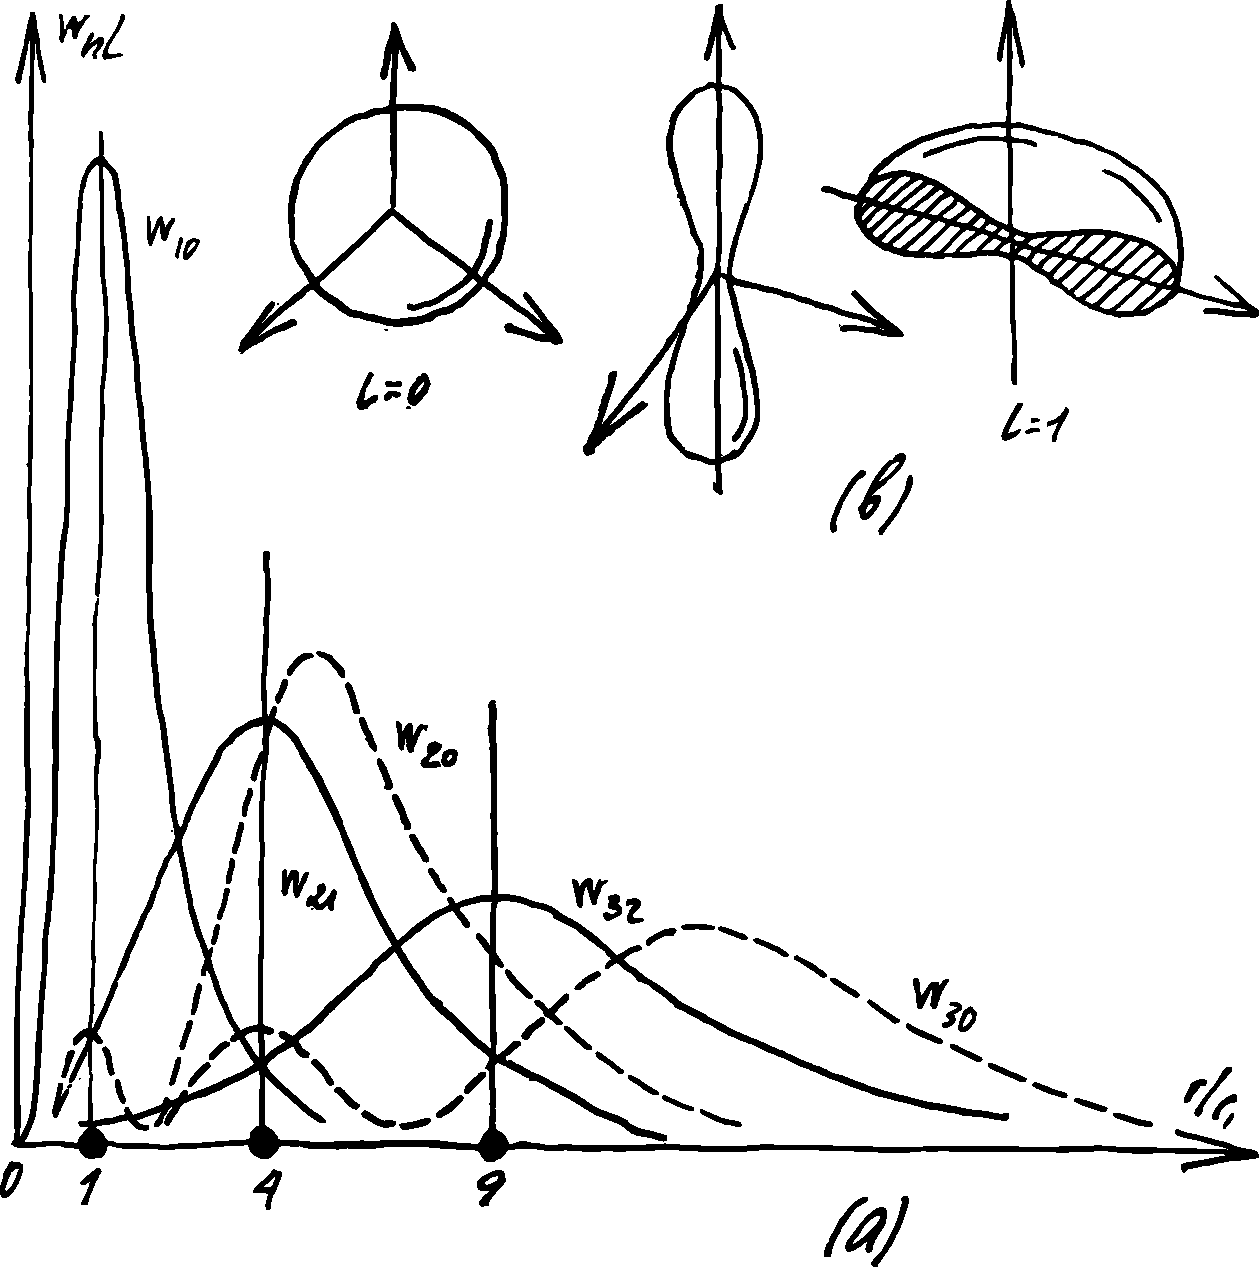
\includegraphics[width=0.7\linewidth]{figures/fig-05-02.pdf}
\caption{Different states of the electron in a hydrogen atom.}
\label{fig-5.2}
\end{figure*}

In \hyperref[fig-5.2]{Figure \ref{fig-5.2} (a)} are shown forms of
functions $w_{nl} (r)$ for different states of the electron in a
hydrogen atom. Notice that the functions $w_{10}, w_{21}, w_{32}$ have
maxima corresponding to the radii of first, second and third orbits in
Bohr's theory. \hyperref[fig-5.2]{Figure \ref{fig-5.2} (b)} shows
forms of function $Z_{lm}$ for some states of the electron. For $l =
0$ (for the so-called $s$-electron) we have a spherical electron
cloud. For $l= 1$ (for $p$-electron) the electron cloud has a form of
either a spindle or a toroid depending on the quantum number $m$. Thus
in order to imagine an electron in atom, one may use conventional
forms like the models of a sphere, spindle, toroid, etc.

The ground state of the hydrogen atom is characterized
 by a spherical electron cloud. Theory shows (see, for example, work
 by Blokhintsev \cite[-1cm]{blokhintsev-1964})
 that in this case 
\begin{equation}%
w_{nl}(r) = 4 \left( \frac{r^{2}}{r_{1}^{3}} \right) \exp \left( -\frac{2r}{r_{1}} \right)
\label{eq-5.4} 
\end{equation}
The parameter $r_{1}$ characterizing the effective radius of the cloud
is determined by relation (\ref{eq-4.4}); in Bohr's theory it occurs as the
radius of the first orbit. 

In conclusion we note that during quantum transitions in an atom,
there occurs not only a change in energy, but also a ``redistribution''
of electron clouds -- a change of their shape and size.


\section{Rejection of Ideas of Classical Physics}
\label{sec-06}
As has \marginnote{General Remarks} been asserted, a transition from
macrophenomena to microphenomena presupposes a rejection of the
basic ideas of classical physics. The notion of a strict continuity in
the spectrum of values of physical quantities is no longer valid,
the classical concept of a tra- jectory is rejected, the principle of
classical determinism is in question. At the root of this viewpoint
lie ideas of quantization (discreteness) and wave-particle duality
which are alien to classical physics.

On the basis of a number of examples that we have considered, we could
see the need to reject the classical principle of unlimited detailing
of objects in space, and of phenomena in time. Thus the question of
the internal structure of elementary particles turns out to be
groundless. Likewise the efforts towards a detailed development in
time of the process of the quantum jump (quantum transition) have no
meaning.


The concepts of energy momentum, angular momentum which are widely
used in classical physics are carried over to quantum mechanics as
well. However, these concepts are now seen differently with a
reconsideration of the previous interconnections, taking into account
the possibility of quantization, and the limitations imposed by the
uncertainty relations. In particular, there arises the question,
unknown to classical physics, of the simultaneous measurement of
physical quantities, and questions about the state and the methods of
describing a state are put in a new light. In conclusion we stress the
impossibility of the classical interpretation of a microparticle, and
the loss of the clarity of classical physics.


The rejection \marginnote{Identity of Microparticles} of the classical
individualization of an object is quite fundamental. In classical
mechanics objects are known to have individuality since it is always
possible in principle to enumerate them and observe the behaviour of
anyone of them. In this case, however alike two classical objects
may be, they are never identical and can always be distinguished. But
in quantum mechanics two microparticles of the same type should be
treated as absolutely identical. Thus, all electrons are identical and
so are all unexcited hydrogen atoms, helium nuclei, etc.

\begin{fullwidth}
  \setlength{\leftskip}{3cm} \textsf{\small Suppose we have several
    electrons, one of which is ``assigned'' the number 1 at the moment
    of time $t= 0$. Can this electron be identified after a certain
    time $t$? Such an identification could have been easily done if we
    could put some ``label'' on this isolated object. We could get by
    without ``labelling'' this electron if we could simply keep a
    watch over the isolated object, i.e. if we could ``mentally''
    follow it (in our imagination) along its trajectory. This is
    precisely what we would have done in the case of isolated
    classical objects. However, none of this holds in the case of an
    electron; it is in principle impossible to ``label'' it. Strictly
    speaking, it has no trajectory. The electron ``isolated'' by us at
    the instant $t = 0$, cannot be isolated in actual practice: it
    does not have the individuality which would allow it to be
    identified in the assembly of electrons after a certain time~t:
    Two electrons are much more ``like each other'' than the
    proverbial ``two peas in a poll''; since the latter are classical
    objects, they could differ in size or in chemical composition in
    some way.}

\end{fullwidth}
\vspace{5pt}
\setlength{\leftskip}{0pt}


It is understood that the identity of microparticles does not exclude the possibility of their differentiation on the basis of different states in which these particles may he found. Two electrons belonging to two different atoms are, of course, identical but at the same time distinguishable. The affiliation of an electron to one atom or another permits its ``isolation''. However, nothing changes physically if the electrons interchange places. It is clear that if such an exchange is possible, for example, by combining the atoms under consideration into a molecule, the distinguishability of the electrons vanishes.


Laplacian \marginnote{Chance and Necessity in the Behaviour of a
  Microparticle}determinism excludes the element of chance from the
behaviour of an isolated object; in classical mechanics,
\emph{necessity} completely dominates. Because of this, the laws of
classical mechanics are \emph{dynamic} and \emph{not statistical}. The
element of \emph{chance} (and, consequently, \emph{statistical laws}
also) appear in classical physics only when considering aggregates of
objects or assemblies of particles.


From this point of view, it is important to stress that in quantum
mechanics we are dealing with a qualitatively different situation
concerning the behaviour of individual microparticles: here, elements
of necessity, as well as chance, are present. An excited atom
\emph{spontaneously} returns to the ground state without any external
influence. This is associated with the spontaneous transitions of
electrons in the atom from one set of energy levels to another. It is
impossible in principle to indicate precisely when a particular
excited atom will return to its ground state; such a return is a
random act. Precisely in the same way, it is impossible to predict
exactly when a given elementary particle, for example, a neutron, will
decay spontaneously. In this case also an element of chance is
present.


In addition to elements of chance, there are also present the elements
of necessity in the behaviour of a microparticle. As has already been
indicated in \hyperref[sec-01]{Section \ref{sec-01}}, if we have
$N_{0}$ neutrons at the instant $t=0, \; N_{0} \gg 1$, we can confidently
state that at the time $t$ we will be left with only $N_{0} \exp
\left( - \dfrac{t}{\tau} \right)$ neutrons, $\tau$ being a constant called the
lifetime of the neutron. Here, the necessity is obvious. In the case
of an individual neutron this necessity is replaced by a definite
probability of keeping the neutron intact until time $t$, once it has
managed to survive to time $t = 0$. This probability is equal to $
\exp \left( - \dfrac{t}{\tau} \right)$. It should be noted that this probability is
independent of the time for which the given neutron has survived up to
the time $t =0$. Necessity is also manifested in the conservation laws
which govern decay processes as well as the processes of
interconversion of microparticles in general. We may also mention the
fact that there are definite modes of decay; for example, a free
neutron may decay into a proton, an electron and an electronic
neutrino.

The existence of chance as well as necessity in the behaviour of an
individual microparticle has very important consequences. It leads to
the fact that quantum mechanics turns out to be in principle a
statistical theory with probability as one of its basic attributes. As
Fock has remarked \cite{fock-1957}, \emph{in quantum physics the
  concept of probability is a primary concept and plays a fundamental
  role.} It could be said that the behaviour of an individual
microparticle is random, but the probability of this behaviour is
necessary.\sidenote{Here, it is quite appropriate to recall the words
  of F. Engels: \emph{Necessity emerges from within the framework of
    randomness}.} The electronic cloud considered in
\hyperref[sec-05]{Section \ref{sec-05}} may serve as a good example of
this. The occurrence of an electron at some point near the nucleus is
a random event, but the probability of its being found at a given
point $(r, \theta, \varphi)$ is definite -- it is described by a
function of the type (\ref{eq-5.3}) Of, in other words, is determined
by the shape and size of the corresponding electron cloud.

In the end, we note that the element of chance in the behaviour of an
individual microparticle is due to the uncertainty relations. In
\hyperref[sec-04]{Section \ref{sec-04}}, we concluded on the basis of
relation (\ref{eq-3.3}) that it is impossible to ``aim a microparticle
to hit a given point''. In other words, the registration of a
particular electron at some point of a detector screen is random; we
can only speak of the probability of such a fact. In
\hyperref[sec-03]{Section \ref{sec-03}}, we introduced on the basis of
relation (\ref{eq-3.2}) the concept of the virtual transitions of a
microparticle. It is easy to see that such transitions also point,
towards the existence of randomness in the behaviour of a
microparticle. When discussing the specific nature of the physics of
microparticles, it is necessary to discuss in greater detail the idea
of virtual transitions and of virtual microparticles associated with
them.


Perhaps \marginnote{Virtual Transitions and Virtual Microparticles}
there is nothing more alien to classical physics than the idea of
virtual transitions and virtual microparticles. The virtual transition
of an electron from level $E_{2}$ to level $E_{1}$ and back (the
transition $E_{2} \to E_{1} \to E_{2}$) may be considered as a process
in which the electron emits and absorbs a photon of energy ($E_{2} -
E_{1}$). Such a photon is called virtual. In contrast to the photons
participating in real transitions, virtual photons cannot be observed
experimentally. The creation of a virtual photon is not connected with
an absorption of energy from outside, and its annihilation is not
connected with a release of energy. The law of conservation of energy
is not violated since a virtual photon exists for a very short time
$\Delta t$ and, according to uncertainty relation (\ref{eq-3.2}), the
energy of an electron emitting the virtual photon is characterized by
the uncertainty $\Delta E \ge \dfrac{\hbar}{\Delta t}$, which may be
of the order of, or greater than, the energy of the photon ($E_{2} -
E_{1}$). The emission or absorption by an electron of virtual photons
corresponds, from a physical point of view, to the process in which an
electron undergoes virtual transitions.

Taking into consideration the emission and absorption of virtual
photons by an electron, one may imagine that each electron is
surrounded by a photon cloud. This ``cloud'' should be compared with the
electron's own electromagnetic field. Two electrons may exchange
virtual photons. In quantum field theory, the interaction of electrons
is seen as a result of the exchange of virtual photons between
electrons. For this we frequently make use of Feynman's diagrams,
which enable us to consider the various processes of photon exchange.

\hyperref[fig-6.1]{Figure \ref{fig-6.1}} shows four Feynman's
diagrams demonstrating the scattering of one electron by another. The
solid lines "show" electrons and the dotted one-photons. The
intersections of solid and dotted lines are called the vertices of the
diagram. 

\begin{marginfigure}%[6.5cm]%
\centering
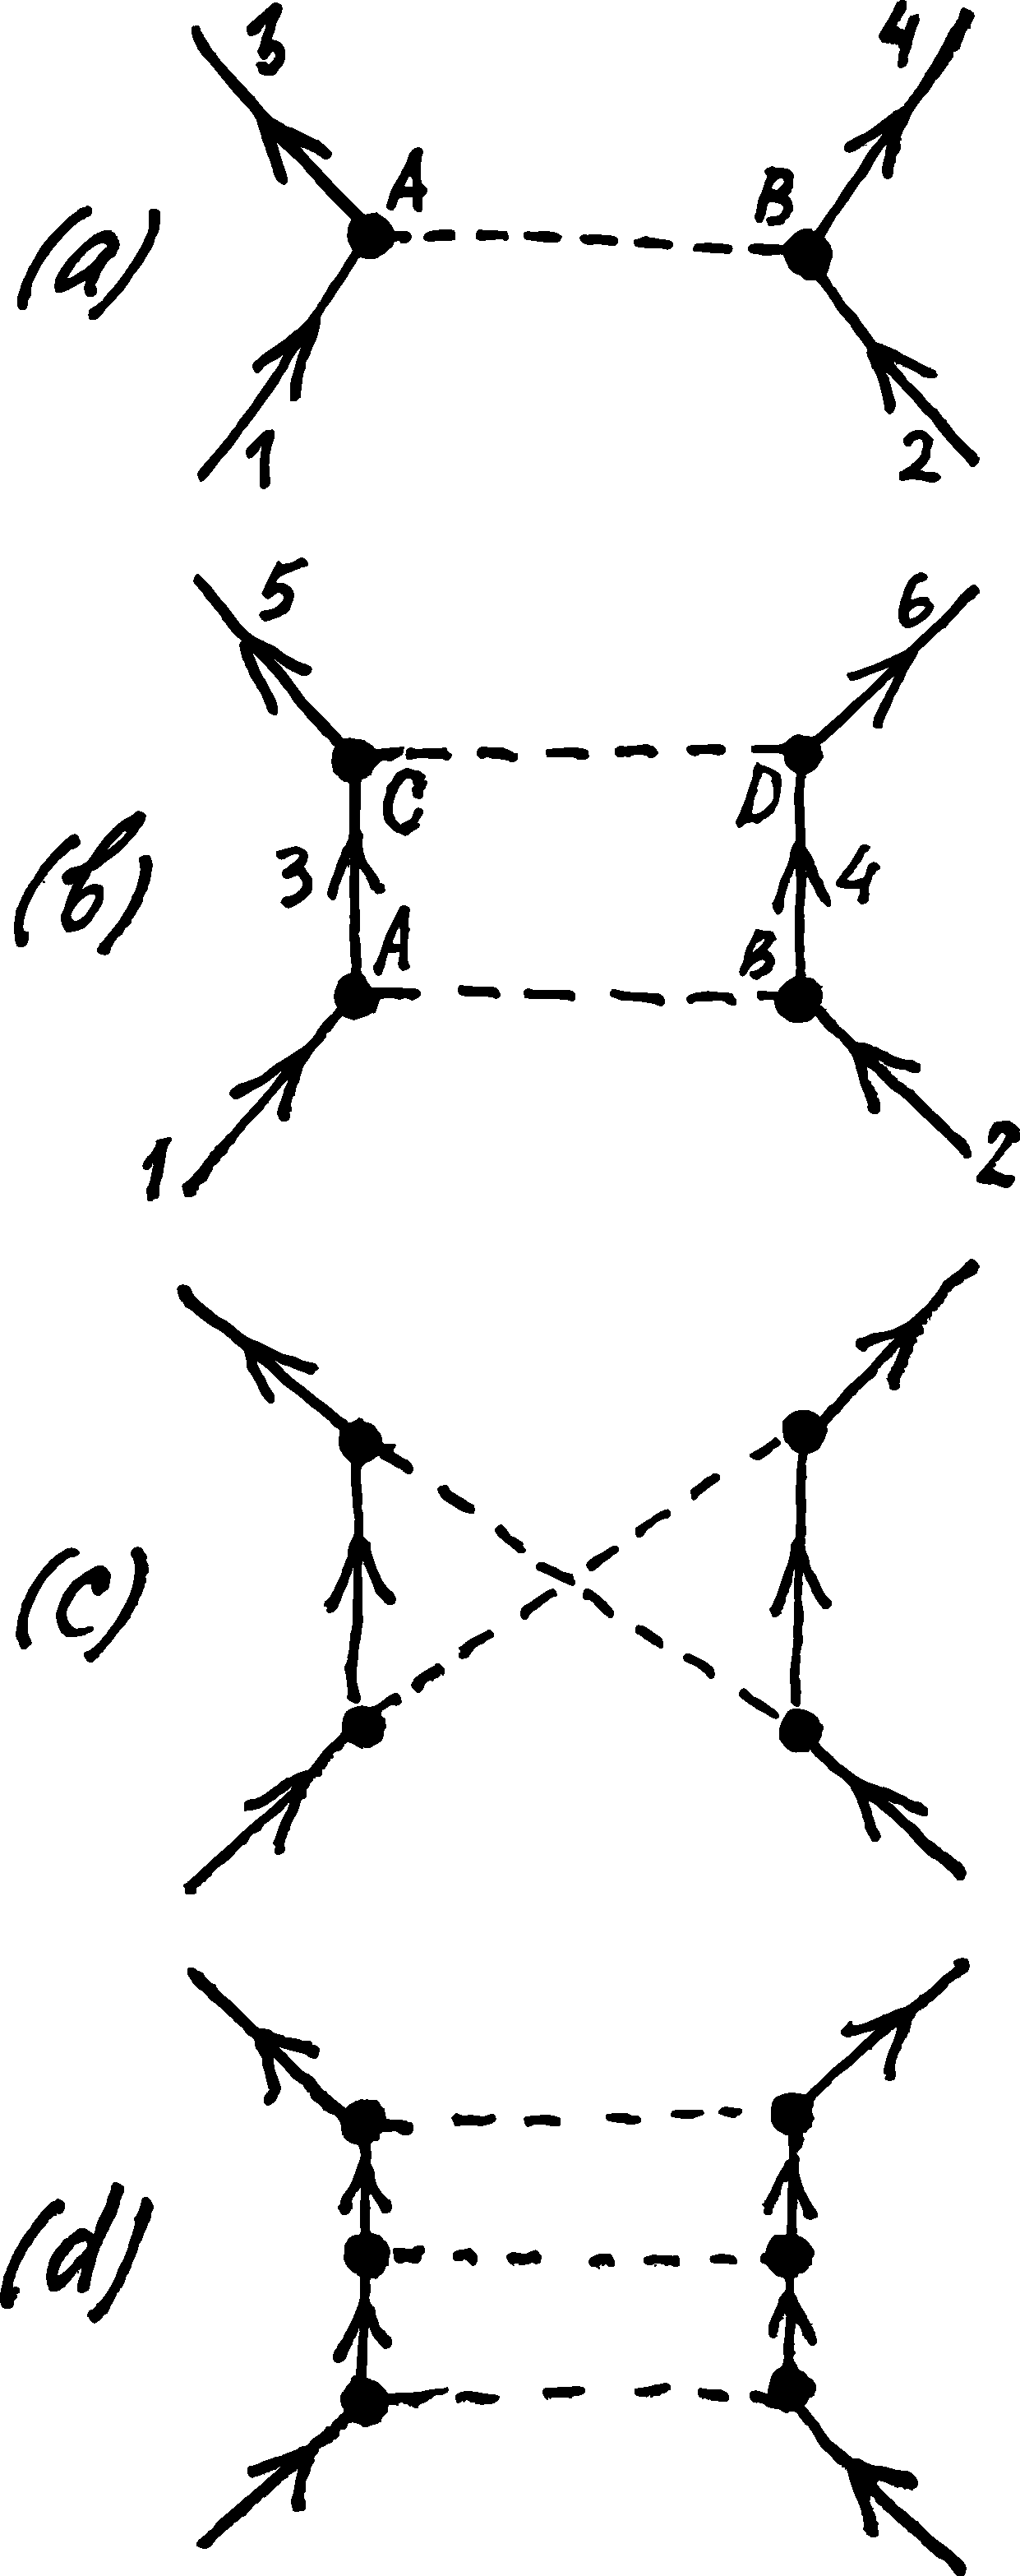
\includegraphics[width=0.9\linewidth]{figures/fig-06-01.pdf}
\caption{Scattering of electrons as shown in Feynman diagrams.}
\label{fig-6.1}
\end{marginfigure}


Let us consider the diagram \emph{(a)}. Here 1 and 2 are the electrons
before interaction with each other (before scattering), $AB$ is a
virtual photon which is exchanged by the electrons during the process
of interaction (note that all the particles indicated in the diagram
by lines connecting two vertices are virtual); 3 and 4 are the
electrons after scattering. Let us turn to the diagram $(b)$. Here 1
and 2 are electrons before scattering, $AB$ and $CD$ are virtual
photons exchanged by the electrons, 3 and 4 are virtual electrons, 5
and 6 are electrons after scattering. The diagram \emph{(c)} is of the
same type as diagram \emph{(b)}; here the electrons exchange two
photons. The diagram \emph{(d)} shows one of the processes in which
the electrons exchange three photons. It is obvious that there is an
infinite number of such diagrams which become more and more
complicated (with the participation of more and more photons).


In order to calculate the probability of scattering of an electron by
an electron, one must consider in principle the contribution of the
various processes indicated by the various diagrams. Fortunately, the
contribution of different processes is different: it is less if the
number of vertices is greater (i.e. if more virtual photons take part
in a process). Theory shows that this contribution is quantitatively
determined by the dimensionless quantity $\left( \dfrac{e^{2}}{\hbar
    c}\right)^{\frac{n}{2}}$, where $e$ is the charge of the electron,
$c$ is the velocity of light, $\hbar$ is Planck's constant and $n$ is
the number of vertices in the diagram. Since $\dfrac{e^{2}}{\hbar} =
\dfrac{1}{137}$, it follows that the main contribution to the
scattering of one electron by another must come from the diagram
\emph{(a)} with two vertices (exchange of one photon). The four
vertices diagrams \emph{(b)} and \emph{(c)} (exchange of two photons)
should provide the next approximation; their contribution will be two
orders of magnitude lower. Thus, in actual practice there is no need
to consider a very large number of diagrams, it is sufficient to limit
ourselves to diagrams with a relatively small number' of vertices.


Of course, a systematic study of Feynman's diagrams and. calculations
based on them is beyond the scope of this book. These questions are
related not to quantum mechanics, but to \emph{quantum field theory}
(quantum electrodynamics)\sidenote{A simple and detailed account of
  Feynmans diagrams is given, for example, in
  \cite{cooper-1968}}. However, a general introduction to the ideas
forming the bases of Feynman's diagrams is quite appropriate at this
point, since they permit us to emphasize the specific nature of the
physics of microparticles and also demonstrate some fundamental
quantum-mechanical principles (the latter will be considered below, in
particular, in \hyperref[sec-25]{Section \ref{sec-25}}).

\begin{marginfigure}[1cm]%
\centering
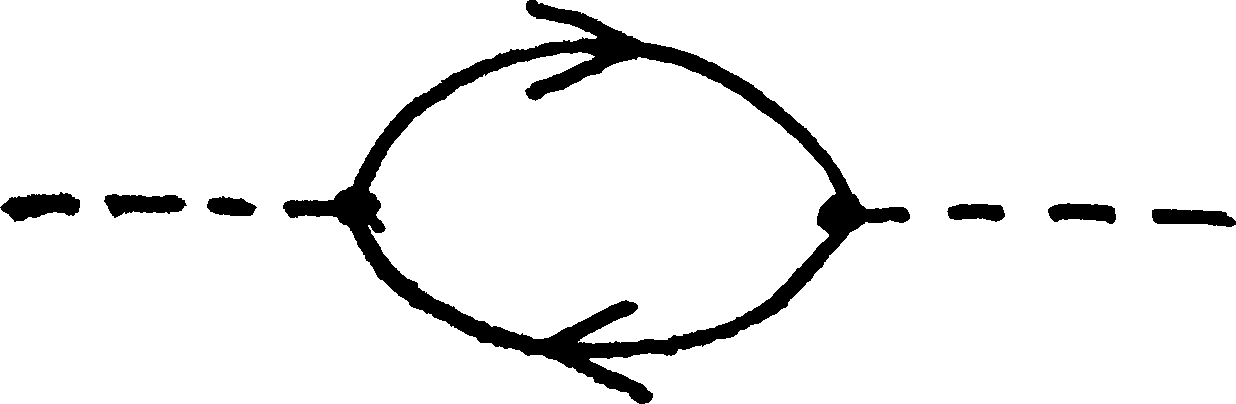
\includegraphics[width=0.8\linewidth]{figures/fig-06-02.pdf}
\caption{Virtual creation of electron-positron from a photon.}
\label{fig-6.2}
\end{marginfigure}


Before ending this discussion on Feynman's diagrams, we consider the
so-called effect of polarization of a vacuum. Figure 6.2 shows a
diagram describing one of the processes responsible for this effect. A
photon is transformed into a virtual electron-positron pair, which is
annihilat- ed and transformed again into a photon (one of the solid
lines between the vertices of the diagram ``shows'' a virtual
electron, and the other, a virtual positron). The members of this pair
during their lifetime may obviously generate virtual photons and,
consequently, new virtual electron-positron pairs, and so on. As a
result of this, the vacuum turns out to be not ``empty'') but
``filled'' with virtual electric charges which must exercise a
screening effect on external (real) charges. Experimental confirmation
of this effect is the best evidence of the usefulness of our concept
of virtual particles.

As \marginnote{The Microparticle and Its Surroundings} we have already
mentioned, the existence of the element of chance in the behaviour of
a microparticle is one of its most specific properties. As a result of
this, quantum mechanics turns out in principle to be a statistical
theory operating with probabilities. But what is the \emph{reason} for
the existence of an element of chance in the behaviour of a
microparticle?

This question can be answered as follows: The existence of chance in
microphenomena is explained by the fact that a microparticle,
figuratively speaking, interacts with all its surroundings. The
specific nature of quantum mechanics is such that, strictly speaking,
not a single object in it can be considered to be fully isolated,
completely independent of its surroundings. It has been
remarked\cite{myakishev-1973} that the cause of the statistical nature
of quantum mechanics is the same as in classical statistical
mechanics, i,e. the existence of a large number of bonds affecting the
motion of the object. A particle treated as free in quantum mechanics
is in fact free only from influences of a dynamic nature. But it
remains under the influence of random forces which cause quantum
fluctuations in its behaviour, as reflected by the uncertainty
relation.

What is the \emph{nature} of the random influences on a microparticle? In
quantum field theory, it manifests itself in an explicit form as the
interaction of a microparticle with a vacuum (recall that a vacuum is
not ``empty''; it is ``filled'' with virtual charges). It may be said that
a microparticle interacts with its surroundings through virtual
microparticles.

The reader should now find it quite natural to interpret wave-particle
duality as the potential ability of a microparticle to exhibit one
kind of property or another, depending on the external conditions,
i.e. on the microparticle's surroundings. This envisages a close
connection between the microparticle and its surroundings-in fact, the
very nature of a microparticle is displayed in one form or another
depending on specific conditions and circumstances.

The impossibility of an unlimited detailization of objects and
phenomena being displayed in quantum mechanics should also be
explained by the interaction of a microparticle with its
surroundings. This means that after a certain stage of investigation,
physical objects cannot be considered as being isolated. Here it is
appropriate to recall the statement given in \hyperref[sec-03]{Section
  \ref{sec-03}} regarding the discussion on quantum transition:
``During the interaction of an electron with photons there is,
strictly speaking, no electron and no photon but a single entity which
must be considered as such without going into details.''

Quantum mechanics reestablishes the idea acquired through everyday
experience regarding the unity of the universe and general connections
among phenomena. This idea received a setback in the classical
theory. The sharp boundaries that existed between waves and particles,
particles and fields, object under investigation and the medium are
all obliterated and the concept of the interconversion of matter is
introduced. We find ourselves in full agreement with the following
appropriate remark made by Bohm:
\begin{quote}
  It seems necessary to give up the idea that the world can correctly
  be analysed into distinct parts, and to replace it with the
  assumption that the entire universe is basically a single,
  indivisible unit. Only in the classical limit can the description in
  terms of component parts be correctly applied without
  reservations. Wherever quantum phenomena play a significant role, we
  shall find that the apparent parts can change in a fundamental way
  with the passage of time, because of the underlying indivisible
  connections between them. Thus, we are led to picture the world as
  an indivisible, but flexible and everchanging, unit.\cite{bohm-1951}
\end{quote}
\clearpage
\section*{Interlude: Is a ``Physically Intuitive'' Model of a Microparticle Possible?}
\addcontentsline{toc}{section}{Interlude: Is a ``Physically Intuitive'' Model of a Microparticle Possible?}
\label{interlude-02}
\paragraph{}
\begin{Verbatim}[formatcom=\color{darkgray},fontsize=\small]
It may well be that these electrons
Are worlds just like our very own,
With kings and scholars, arts and armies,
And memories of ages flown.
And atoms-cosmic systems, spinning
Around a central spinning sphere.
Where things are just like ours, but smaller, 
Or nothing like what we have here.
Bryusov The World of the Electron
\end{Verbatim}


\vspace{8pt}




\textsc{Author:} The impossibility \marginnote{Participants: (same as
  in Prelude).} of the classical interpretation of a microparticle
predetermines a negative answer to the question ``Is it possible to
have a ``physically intuitive'' model for a microparticle?''
\\
\textsc{Classical Physicist:} It is still not clear why a ``physically
intuitive'' model,of a particle explaining its various properties
including spin, instability, wave properties, etc. cannot be
created. Such a model may turn out to be complicated. Or, it may be
possible that we still do not know enough about a microparticle to
create such a model.  But why can't we believe in the very possibility
of this model?
\\
\textsc{Author:} There are very sound reasons for this. I shall
indicate just two of them. Firstly, any modelling envisages in the
long run a detailization irrespective of whether it is a model of an
object or a process. However, the impossibility of an unlimited
detailization is characteristic of microparticles and microphenomena,
as we have already mentioned. This important situation was
persistently stressed by Bohr. He wrote, in particular (see his
article \emph{Quantum Physics and Philosophy}):
\begin{quote}
  A new epoch in physical science was inaugurated, however, by
  Planck's discovery of the elementary quantum of action, which
  revealed a feature of wholeness inherent in atomic divisibility of
  matter. Indeed, it became clear that the pictorial description of
  classical physical theories represents an idealization valid only
  for phenomena in the analysis of which all actions involved are
  sufficiently large to permit the neglect of the quantum \ldots \cite{bohr-1963}
\end{quote}

It is appropriate to mention here that this feature of wholeness
indicated by Bohr is closely linked with the identity of a
microparticle. Secondly, as we have already indicated, a
characteristic property of microparticles is their inavoidable
interaction with surroundings leading, in particular, to a dependence
of some of the properties of microparticle on definite external
circumstances. These properties should be treated as certain
possibilities which can be realized depending on the external
circumstances. One may ask, in what way can these possibilities be
reflected in the framework of a definite "physically intuitive" model?
\\
\textsc{Classical Physicist:} It must be admitted that these ideas
serve as strong arguments against a ``physically intuitive'' model of
a microparticle. However, I don't like the very spirit of quantum
mechanics which rejects graphic representations. In my view it
introduces subjectiveness in describing real world. Take, for example,
the statement: ``The electron may present itself as a wave or as a
particle, depending on circumstances''. Now, everything depends on
circumstances, especially on the circumstances of
observation. Involuntarily, one gets the idea that the electron is not
something objective, but rather something subjective depending on how
we ``look'' at it.
\\
\textsc{Author:} Of course, this is not true. First of all, you
overlook the fact that the electron has quite definite characteristics
like rest mass, electric charge, spin, etc. It is stable and is a
fermion. As regards a ``physically intuitive'' model of an electron,
well, it simply does not exist. However, in rejecting a ``physically
intuitive'' model of a microparticle, quantum mechanics in no way
sacrifices objectivity in favour of subjectivity. It is just that the
electron is a very complicated physical object, and depending on the
external circumstances, including circumstances of observation, it
exhibits its different aspects, which objectively existed in potential
form (I stress this) even before the observer was born. A sober
assessment of this complex situation is that a ``physically
intuitive'' model of the electron is not possible.
\\
\textsc{Classical Physicist:} Can one seriously speak about an object
without having an idea of what it looks like? Isn't it strange that we
study, for example, the behaviour of an electron in a crystal while we
don' t even know what an electron actually is?
\\
\textsc{Author:} I don't agree that we don't even know what an
electron is. I have just indicated a number of precisely determined
characteristics and properties of an electron. More detailed
properties of microparticles in general and electrons in particular
were considered in the preceding sections of the book (and will be
considered in the following sections). In fact, we know quite a lot
about the electron and know, in particular, about its behaviour in a
crystal. This is evidenced by the large number of semiconducting
devices fabricated and used by us in practice. As you will see, the
absence of a ``physically intuitive'' model of the electron has in no
way turned out to be a serious obstacle. We may even go a step further
and state that an understanding of natural phenomena in which Planck's
constant plays an important role is possible only through a
significant rejection of a graphic description. By the way, this idea
was given by Heisenberg, in whose works much attention was given to
questions of the use of physically intuitive methods.
\\
\textsc{Classical Physicist:} But by rejecting models, isn't quantum
mechanics running the risk of losing its material basis? Won't we be
finally left with only equations and abstract mathematical symbols?
\\
\textsc{Author:} I can understand your doubts. For you, apparently,
only the extremes matter: either graphic models, or mathematical
abstraction. To you, either a model should reflect everything or
almost everything, otherwise it is quite useless. The doubts arising
in your mind are a consequence of precisely this type of
viewpoint. However, the quantum-mechanical approach to such questions
is more flexible, or rather, \emph{dialectical}.
\\
\textsc{Classical Physicist:} I don't understand what exactly you mean
by that.
\\
\textsc{Author:} I want to stress two points. Firstly, although there
is no ``physically intuitive'' model for a microparticle, this does
not stand in the way of the ``model representations'' in quantum
mechanics.
\\
\textsc{Classical Physicist:} That means I was right after all?
\\
\textsc{Author:} This is something different. Quantum mechanics
believes that even the most refined model cannot reflect the specific
characteristics of a microparticle, Hence quantum mechanics makes use
of \emph{tentative} models (tentative images) -- sometimes one,
sometimes another, admitting the \emph{relativity} of every model. The
only thing that is important is that each of the models employed
should reflect some side of the nature of the object or
phenomenon. Thus, when considering electronic transitions through the
forbidden band in a semiconductor, we unhesitatingly imagine electrons
as some kind of corpuscles, which ``jump'' on the energy scale. When
considering the propagation of electrons through an ideal crystal
lattice we use wave concepts. It is convenient to study the scattering
of electron waves by the elastic waves of a crystal in a ``corpuscular
language'' using the picture of collisions of corpuscles of two types
-- electrons and phonons.  Similarly, the image of the electron cloud
used for describing electrons in an atom also serves as a good example
of ~tentative modelling. As you see, modelling in quantum mechanics is
used quite extensively and flexibly. More- over, all models are not
interpreted literally but tentatively.
\\
\textsc{Classical Physicist:} All right. And what is your second
point?
\\
\textsc{Author:} The second point is as follows: Quantum mechanics
makes use of both tentative models and mathematical abstractions on an
equal footing. Just on equal footingl At this point modern physics
breaks off quite radically from classical concepts. Stressing the
great heuristic (and leading) significance acquired by mathematics in
the new physics, which was not the case earlier in the epoch of the
domination of ``physically intuitive'' concepts, Vavilov writes:
\emph{we don't have enough accepted ideas and concepts for a
  physically intuitive model interpretation, but logic with its
  immense perspectives represented in mathematical form continues to
  be valid, thereby creating order in the new, unexplored world and
  opening possibilities for physical predictions.}\cite{vavilov-1970}
\\
\textsc{Classical Physicist:} As a matter of fact, there is nothing
definite in all this.
\\
\textsc{Author:} To be more precise, there is nothing predetermined
beforehand. The new physics turns to a study of the objective world,
if one may say so, ``without classical prejudices''. It flexibly makes
use of different media: models and mathematical
abstractions. Figuratively speaking, it is not ``alien to anything
that is human''. Summing up, we may say that firstly, when studying
microphenomena, we do make use of visual models quite
extensively. Secondly, models are by no means taken literally in
quantum mechanics; their relativeness and arbitrariness are
considered. Thirdly, getting acquainted with microphenomena is based
on the \emph{dialectic unity of model concept, and mathematical
  abstractions}.

%\cleardoublepage

% Section 7. Sedion 8.
% Section 9.
% Section 10. Section 11.
% Section 12. Section 13. Section 14. Section 15. Section 16.
% Some Basic Experiments	68 Amplitudes of Transition Probabilities (Formulation
% of Basic Principles)	79 Amplitudes of Transition Probabilities (Demonstra-
% tion of Basic Principles)	84 Superposition of States	96 Measurement in Quantum Mechanics	106 Interlude. Are These the Same Waves? Or, Again
% on Waves in Quantum Mechanics	115 Causality in Quantum Mechanics	117 Microparticles with Two Basic States	123 The Electron in a Magnetic Field	131
% The Wave Function	138 Quantum Mechanics as a Qualitative Leap in Man's
% Knowledge of the Laws of Nature	143
% Interlude. Do Quantum-Mechanical Concepts Con- tradict Our Common Sensel	156

\chapter[Physical Foundations of Quantum Mechanics]{Physical Foundations of \newline Quantum Mechanics}


\begin{figure*}%[1cm]
\centering
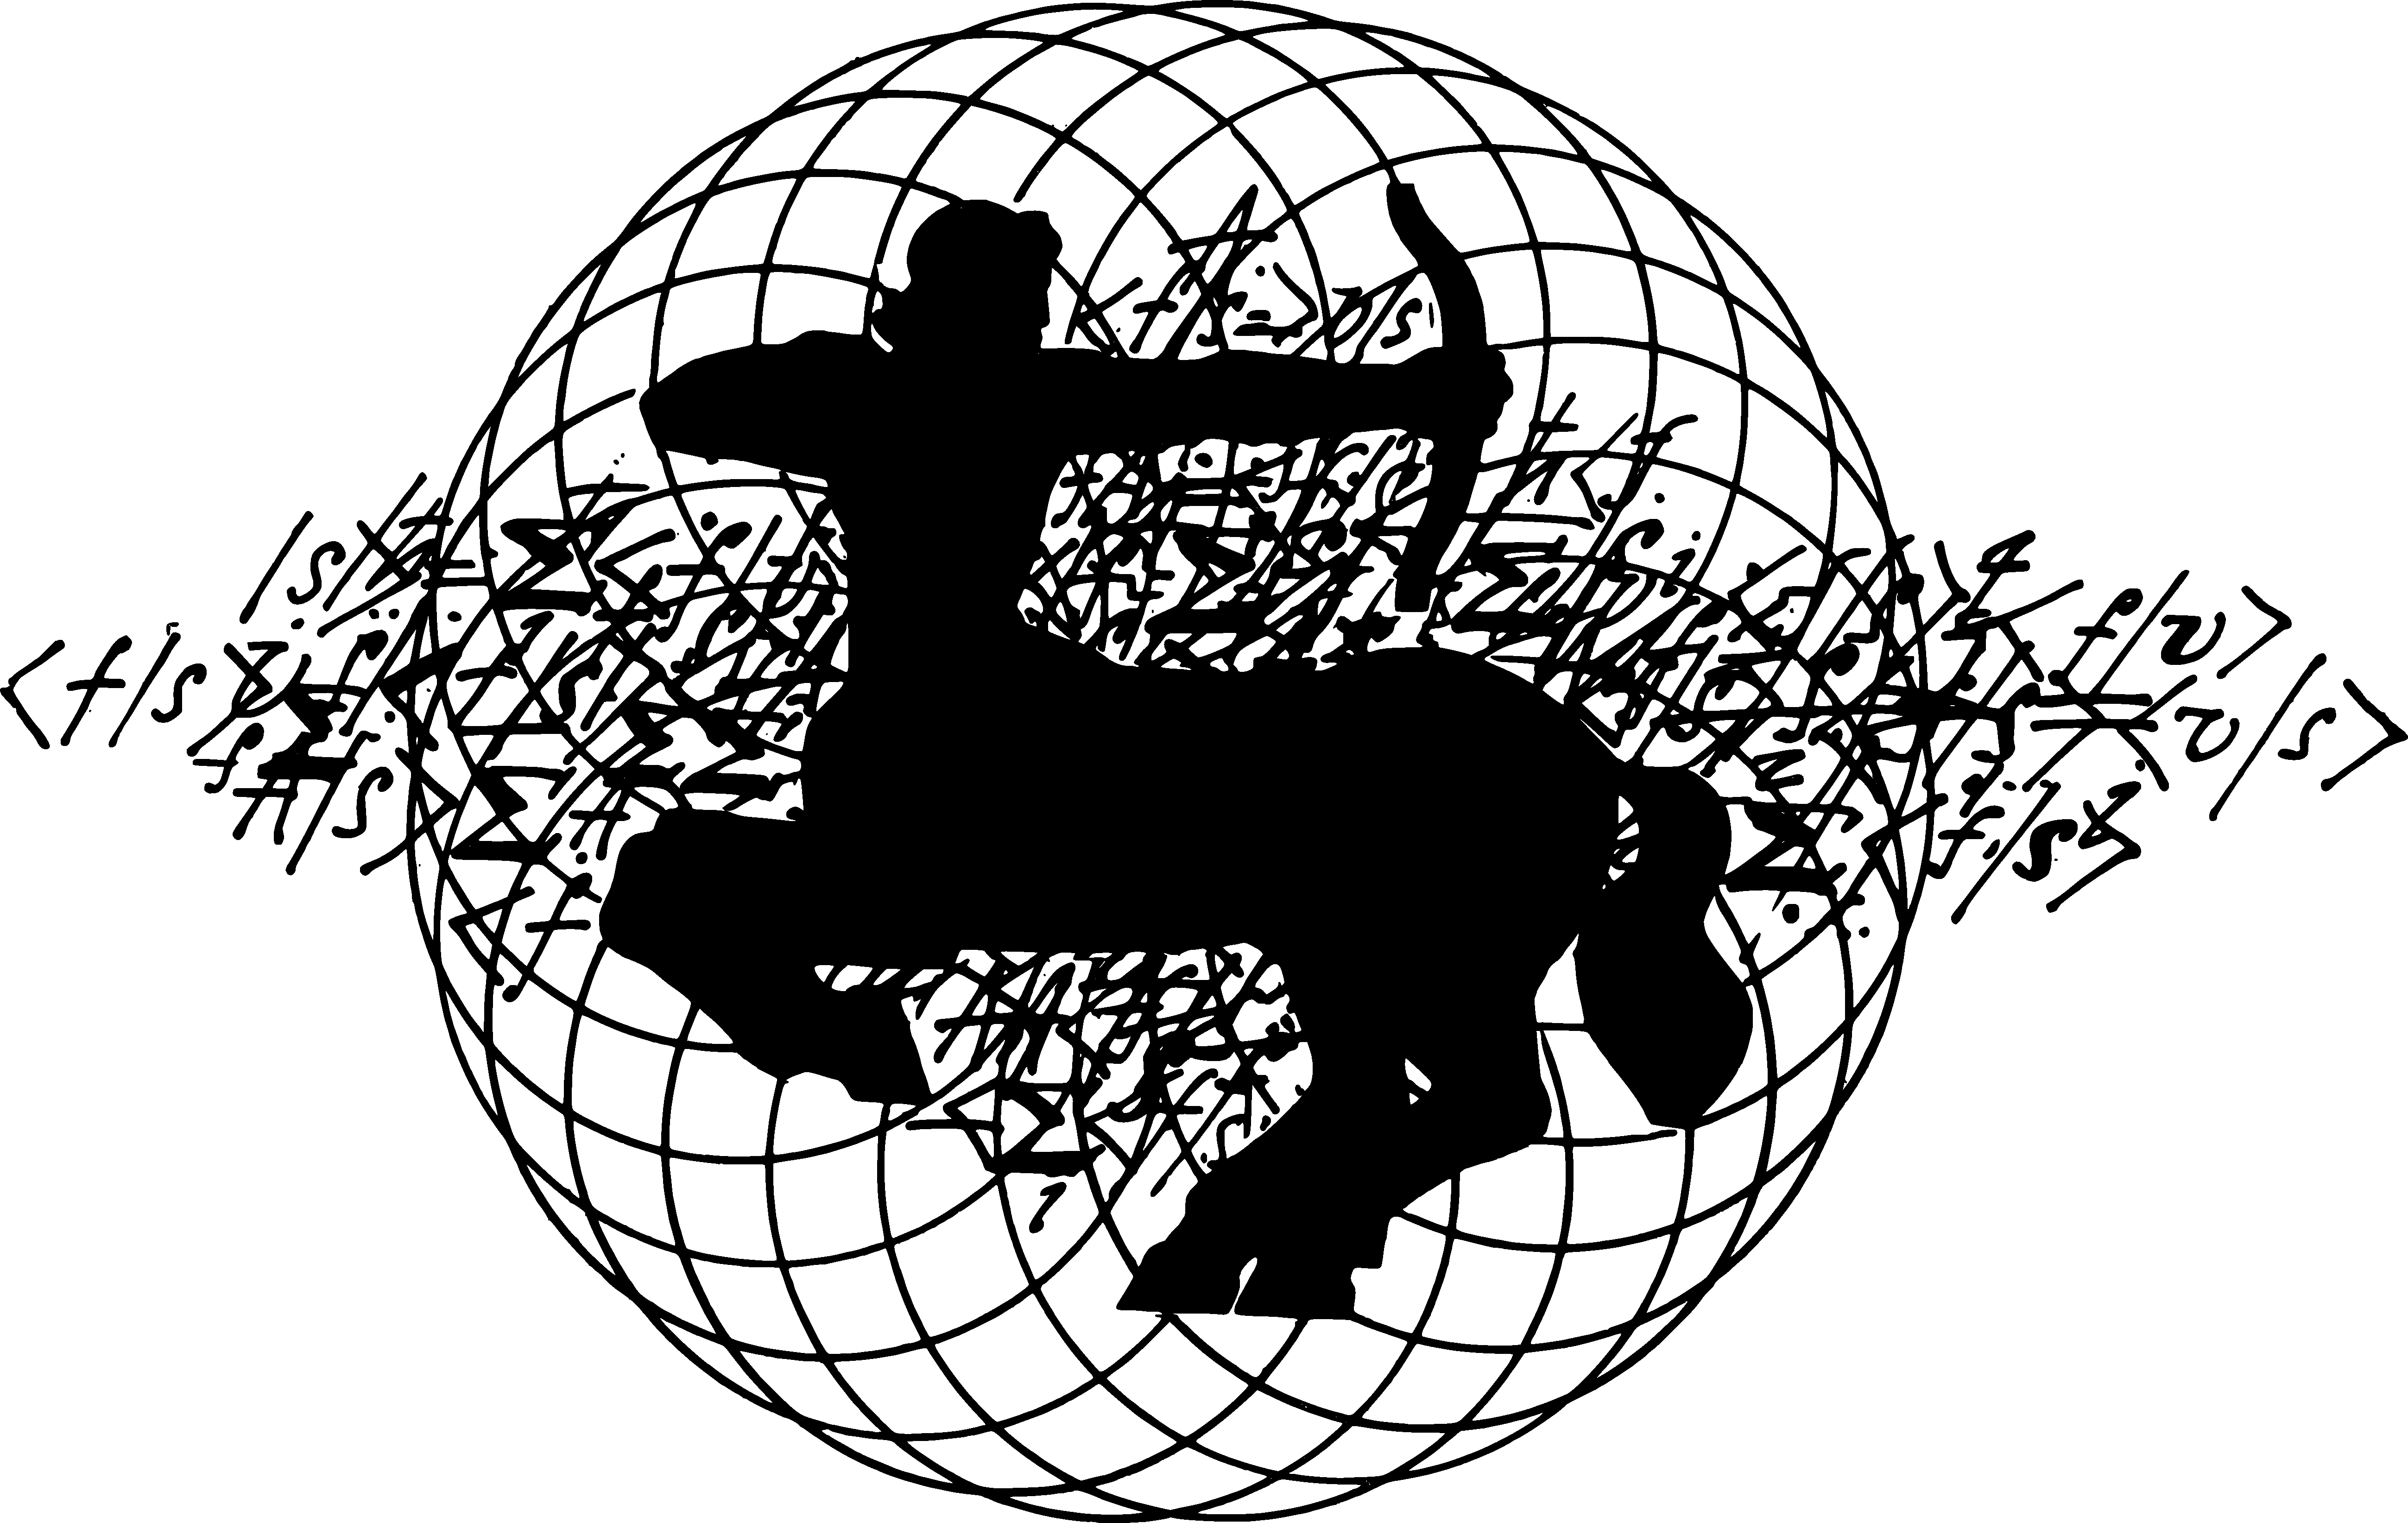
\includegraphics[width=\linewidth]{figures/ch-02.pdf}
%\label{}
\end{figure*}
\cleardoublepage

\section{Some Basic Experiments}
\label{sec-07}
The \marginnote{Actual Experiments and the System of Basic Experiments} concepts of quantum mechanics are based on a vast collection of experimental data gathered over a period of more than fifty years at the end of the 19$^{\mathrm{th}}$ century and in the first half of the 20$^{\mathrm{th}}$ century. Among the large number of experiments, a few stand out as being definite ``milestones'' and can hence be called decisive. They include the experiments of Lummer and Pringsheim on black body radiation coupled with Planck's theoretical works (1900), the experiments of Frank and Hertz (1914) on inelastic collision of electrons with atoms, Millikan's experiments (1914) on the photoelectric effect, confirming the laws predicted earlier by Einstein, the experiments conducted by Stern and Gerlach (1921) on the splitting of atomic beams in non-uniform magnetic fields, the measurements of wavelengths of X-rays scattered by matter carried out by Compton (1923), and the experiments of Davisson and Germer, and Tartakovsky (1927) on electron diffraction.\sidenote{A description of these experiments may be found, for example in \cite{trigg-1971}.} These experiments (and many others which did not become so famous) constitute the foundation on which, over a number of decades, quantum theory was built, perfected, freed from various paradoxes, and finally brought to its present harmonious structure. 

Looking now from the position of the existing quantum theory at the experimental quest which led to it, it is worth generalizing the actual experimental picture by omitting the details that do not play a significant role and trying to conceive the simplest system of basic experiments which describe the fundamental aspects of the quantum-mechanical viewpoint. In this section an attempt has been made to consider such a system of experiments. This system is built on the basis of actual experiments but one should not look for a one-to-one correspondence between the basic experiments and actual experiments conducted at a certain time in a certain laboratory. Basic experiments must be seen as a sort of generalization of several actual experiments. Hence, the experimental details concerning a certain apparatus or various details of a historical nature do not play a significant role here. 

In our view, resorting to the system of basic experiments is motivated by two circumstances. Firstly, being free
from the details of actual experimental researches and their unavoidable ``zigzags'' and ``deadends'', such a system of experiments permits one to isolate the main events prominently, and clearly show the experimental foundations of the theory. Secondly, quantum-mechanical ideas have so radically changed our views on the structure and properties of matter that it would not be proper to draw final conclusions on the basis of particular individual experiments (even on ``decisive'' experiments) but only on their totality. It is essential to reconsider the totality of experiments as a whole, and for this purpose it is useful to conceive a system of basic experiments. 


Let us \marginnote{Experiment 1 (Microparticles in an Interferometer)}begin by considering the well-known experiment on the interference of light waves. \hyperref[fig-7.1]{Figure \ref{fig-7.1}} schematically shows the simplest \emph{interferometer}. Here, \textsf{1} is a point source of monochromatic light, \textsf{2} is a screen with two small slits $A$ and $B$, and \textsf{3} is a detector screen registering the intensity of light impinging it. This intensity indicated on the diagram by the curve $I(x)$. The interference character of the curve $I(x)$ is fairly simply
explained within the framework of classical wave theory of light:  the light wave from source \textsf{1} upon reaching is the screen \textsf{2} converts the slits $A$ and $B$ into sources of new light waves, which add up to give on screen \textsf{3} the characteristic \emph{interference pattern} of intensity distribution.

\begin{marginfigure}
\centering
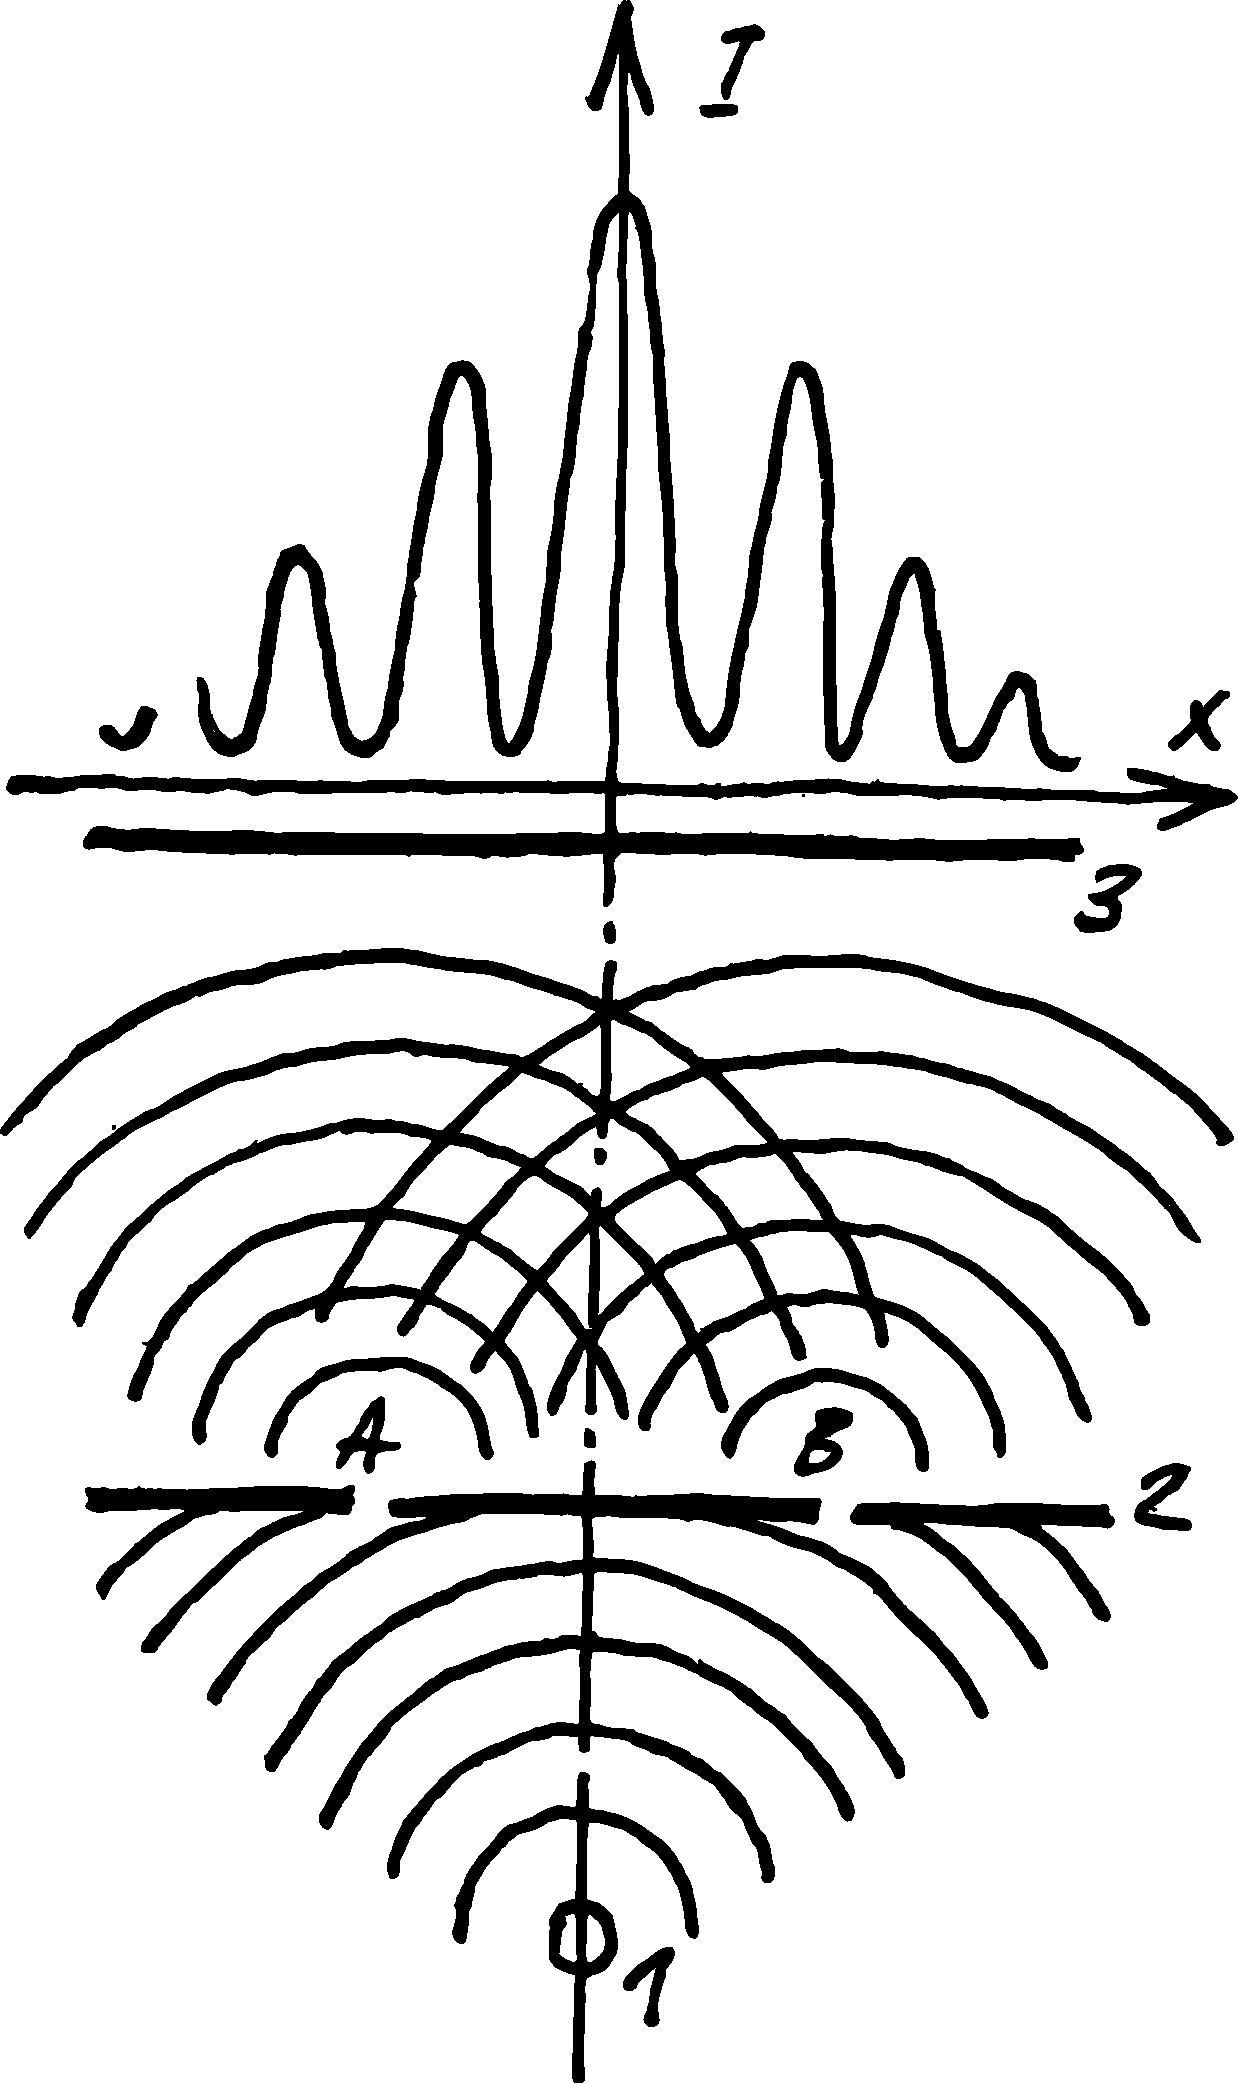
\includegraphics[width=\textwidth]{figures/fig-07-01.pdf}
\caption{The double slit experiment.}
\label{fig-7.1}
\end{marginfigure}

We recall that interference of light was observed in the middle of the 17$^{\mathrm{th}}$ century by Grimaldi, and its explanation on the basis of wave concepts was given in the beginning of the 19$^{\mathrm{th}}$ century by Young. Since then, the experiment shown in  \hyperref[fig-7.1]{Figure \ref{fig-7.1}} is called Young's experiment.


One might ask what relation can the phenomenon of the interference of light, discovered and explained long ago, have with quantum mechanics? It turns out that the two are directly related.


Let us gradually reduce the intensity of light from source \textsf{1}. The illumination of screen \textsf{3} as a result will naturally decrease. However, the interference character of the curve $I(x)$ will be retained. By increasing the time of exposure, it is possible in principle to obtain the interference curve $I(x)$ for even the smallest light intensities. This is not trivial since with decreasing intensity of the light beam the number of photons in it will decrease and so, obviously, a situation should arise when individual photons will have to be considered in place of light waves. However, as has been shown experimentally, the nature of the interference curve $I(x)$ obviously remains unchanged no matter how much the light intensity is decreased. The distribution of the individual photons falling on the detector screen gives the same interference pattern on the screen as is produced by light waves.


Moreover, the interference is observed even if at point \textsf{1} ( \hyperref[fig-7.1]{Figure \ref{fig-7.1}}) we place a source of monochromatic electrons (all having the same energy). In this case also the intensity of the electron beam may be reduced indefinitely. We can even perform an experiment in which the electrons pass through the interferometer one by one. By studying the distribution of the electrons falling on the detector screen over a sufficiently long exposure time we get in this case also the characteristic interference pattern [curve $I(x)$l. Experiments repeated with other microparticles (protons, neutrons, etc.) lead to similar results. From an observation of the behaviour of microparticles in the interferometer it should be concluded that, firstly, the phenomenon of interference is inherent in all microparticles and, secondly, it should be explained by the properties not of \emph{ensembles} of microparticles but of \emph{individual} microparticles.


We shall try to ``follow'' the motion of an individual microparticle (say, electron) in the interferometer shown in  \hyperref[fig-7.1]{Figure \ref{fig-7.1}}. The electron emerges from point \textsf{1}, passes through the slits in screen \textsf{2} and is finally registered at a certain point $x$ on screen \textsf{3}. By repeating the experiment for a large number of single electrons we notice two fairly interesting facts.


The first fact is the impossibility of predicting precisely at what point $x$ a particular electron will be registered. The experimental conditions are the same for each electron (remember that the electrons pass through the interferometer one by one) and yet each electron ``behaves in its own way''; moreover, one cannot predict the way in which it will behave. This remark applies to every single electron. However, by following a large number of electrons, we observe a pattern in the distribution of their incidence on the screen \textsf{3}, shown by a kind of the interference curve $I(x)$. Moreover it is immaterial whether we observe the distribution of the incidences of a large number of single electrons or the distribution of the incidences of electrons from a beam. Thus, the unpredictability concerning the behaviour of an individual microparticle is associated with the predictability concerning the behaviour of a large number of microobjects.

\begin{marginfigure}
\centering
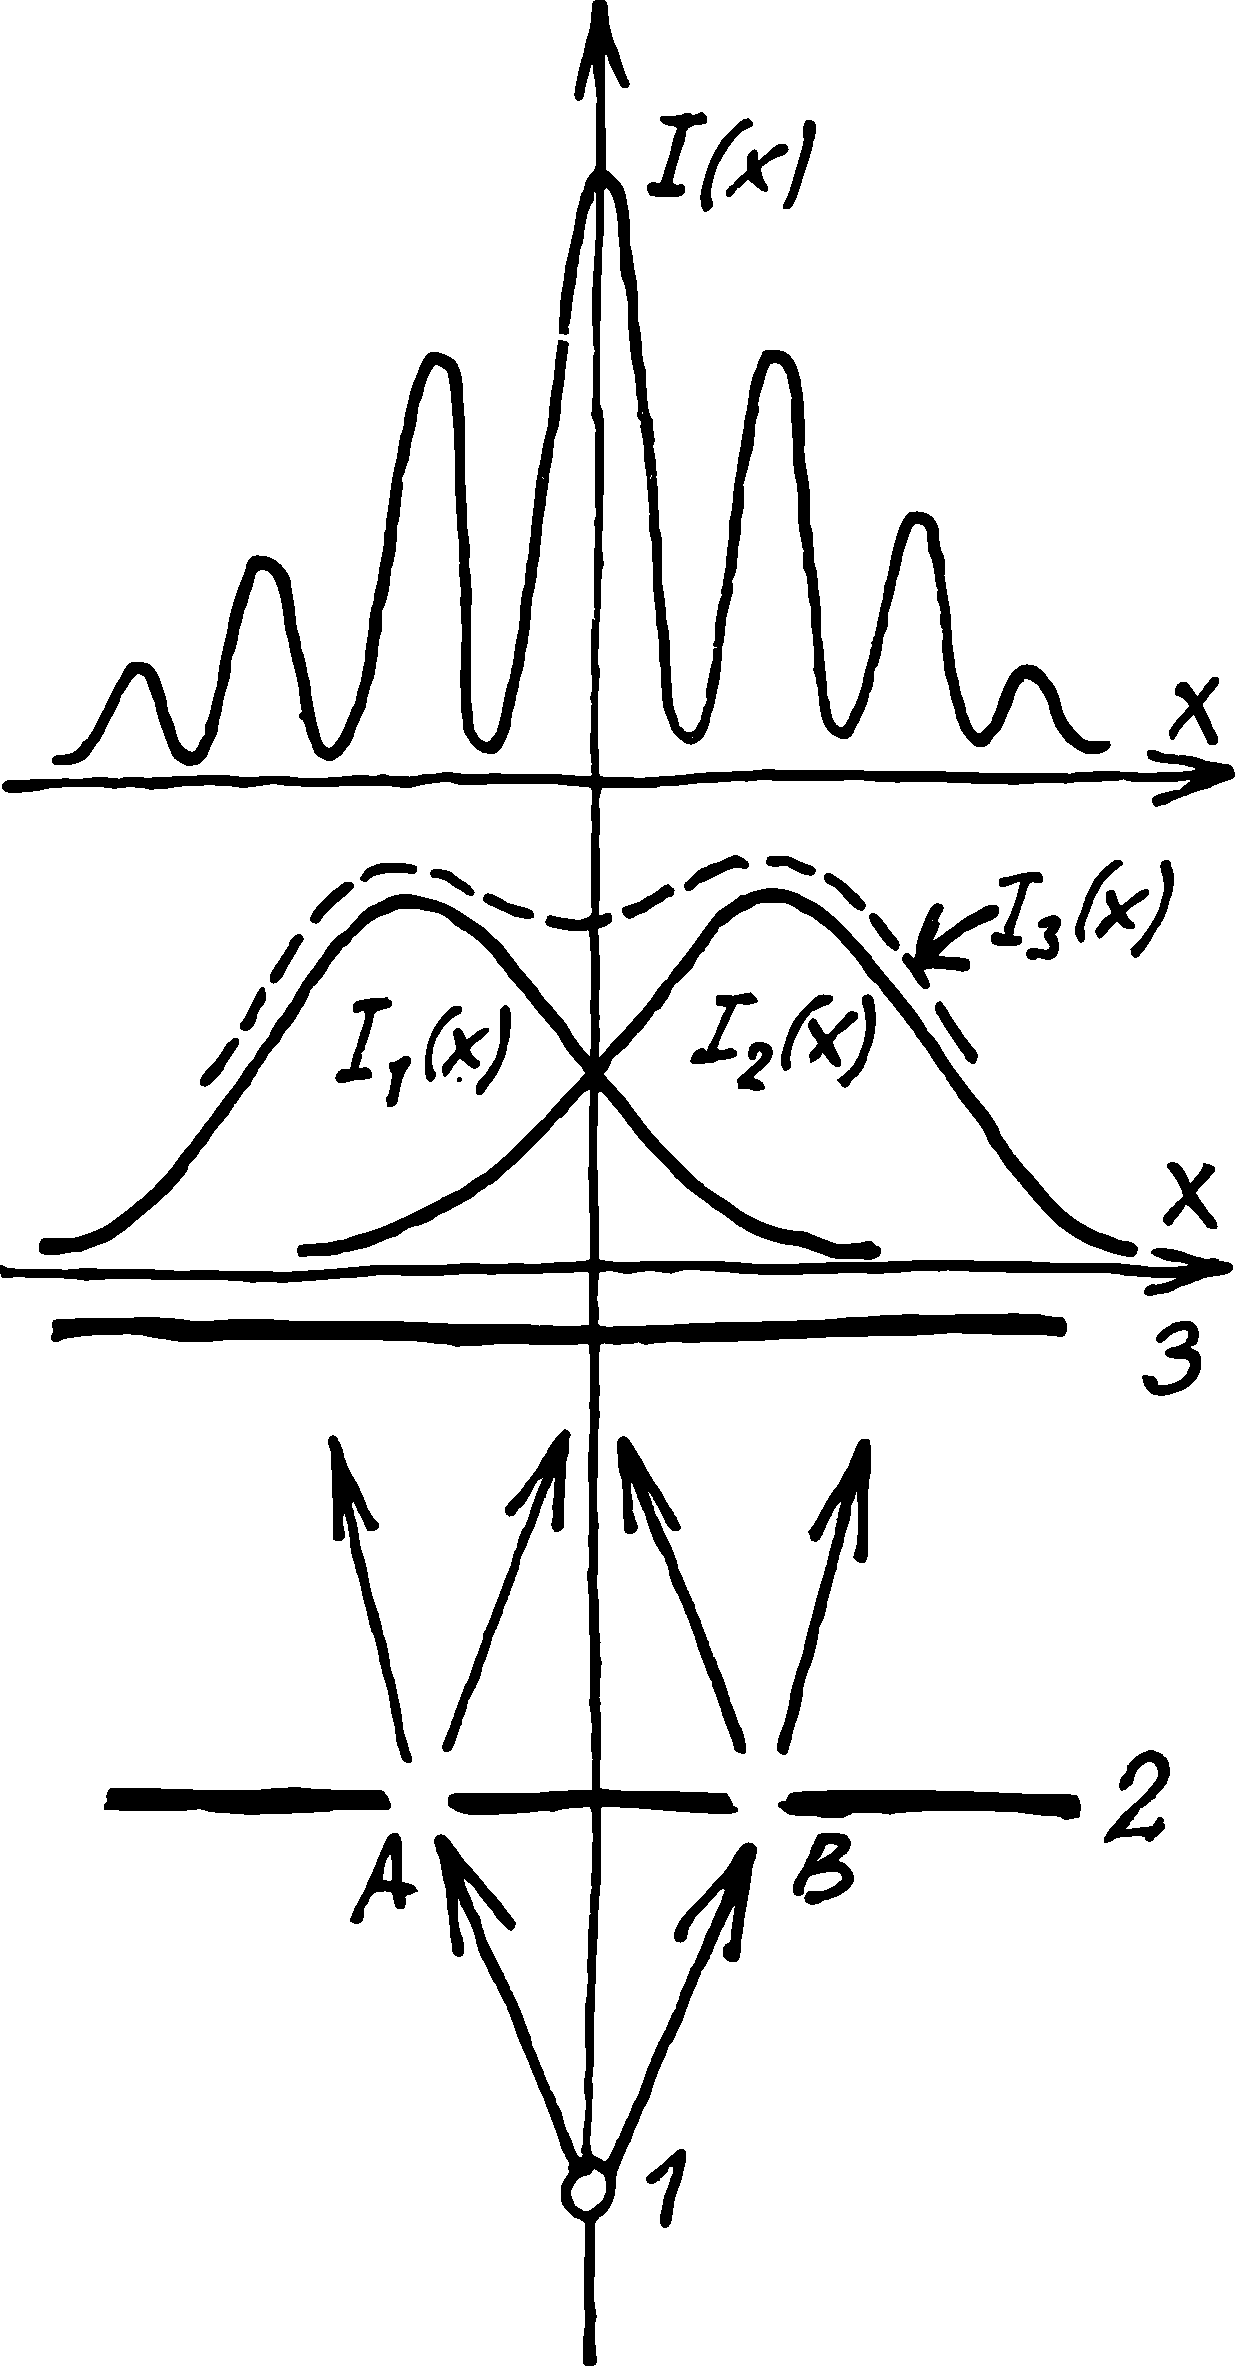
\includegraphics[width=\textwidth]{figures/fig-07-02.pdf}
\caption{The double slit experiment, with one slit closed.}
\label{fig-7.2}
\end{marginfigure}


The second fact is connected with the specific nature of the passage of an electron through the slits in the screen. Let us close slit individual $B$; in this case we observe the distribution of incidences on the screen, as described by curve $I_{1}(x)$ (\hyperref[fig-7.2]{Figure \ref{fig-7.2}}). Let us open slit $B$ but close slit $A$; in this case the distribution $I_{2}(x)$ is observed. By opening both slits, we do not get the additive distribution $I_{1}(x) + I_{2}(x)$ described by the curve $I_{3}(x)$ in the diagram but the interference distribution $I(x)$ which was noted earlier. It is this fact that is especially remarkable. If we suppose that each electron passes through anyone of the slits, the appearance of the interference distribution $I(x)$ forces us to admit that the electron in some way ``perceives'' the other slit, otherwise, it does not matter for an electron passing through one slit whether the neighbouring slit is open or closed and thus the distribution of incidences with both slits open must be described not by the interference curve but by the additive curve $I_{3}(x) = I_{1}(x)+ I_{2}(x)$. The electrons passing through slit $A$ should give the distribution $I_{1}(x)$, while those passing through slit $B$ should give the distribution $I_{2}(x)$. The detector screen should then register the sum of these distributions. Since it is meaningless to talk about the electron ``perceiving'' we have to admit that the interference distribution $I(x)$ observed with both the slits open is associated with the passage of the electron somehow simultaneously through the two slits.


However, this admission does not simplify matters since it is not clear exactly in what way a single electron can pass simultaneously through two slits. Of course, we may assume that the electron at first passes through one slit, then it somehow returns through the other slit and again passes through the first slit (we get a sort of loop encompassing both the slits). Finally, we may assume that near the slits the electron is ``spread out'' (delocalized) in space, partially passing through one slit and partially through the other, and while impinging on the detector screen, it is again localized in space (we get a temporary splitting of the electron into two ``halves''). There is no special need to prove that both the attempts made above to model the passage of electron through two holes are artificial. This becomes quite obvious if we turn to more complicated interferometers. Thus, in Michelson's interferometer, for example, one ``half'' of the microparticle will have to move towards one reflecting mirror and the other ``half'', towards the other (in completely the opposite direction).

Thus, the interference curve $I(x)$ greatly complicates the problem about the nature of the passage of a microparticle through a screen with two slits. If the microparticle passes through one slit, then either there should be no interference, or we must admit that the microparticle has a hidden ability to ``perceive'' the neighbouring slit. The only logical conclusion arising from the existence of interference is that the microparticle passes simultaneously through two slits, though the mechanism of such an unusual passage is not clear. In such a situation, obviously, a direct experiment could be helpful. Why shouldn't we try to ``spy'' on the electron to see exactly in what way an electron passes through the slits in the screen? Such experiments were actually conducted. Let us see what they led to.

Let \marginnote{Experiment 2 (``Observing'' a Microparticle in the Interferometer)} us imagine that near the slits $A$ and $B$ of screen \textsf{2} we have light sources \textsf{4} and photodetectors \textsf{5} (\hyperref[fig-7.3]{Figure \ref{fig-7.3}}), designed for ``observing'' the passage of electron through the screen with slits (the photodetectors register light scattered by the electron). If the electron simultaneously passes through both the slits both the photodetectors are activated simultaneously, But if the electron passes through either one of the slits, only one detector is activated; in this case we shall also know through which slit the given electron passes. 


\begin{marginfigure}[1cm]
\centering
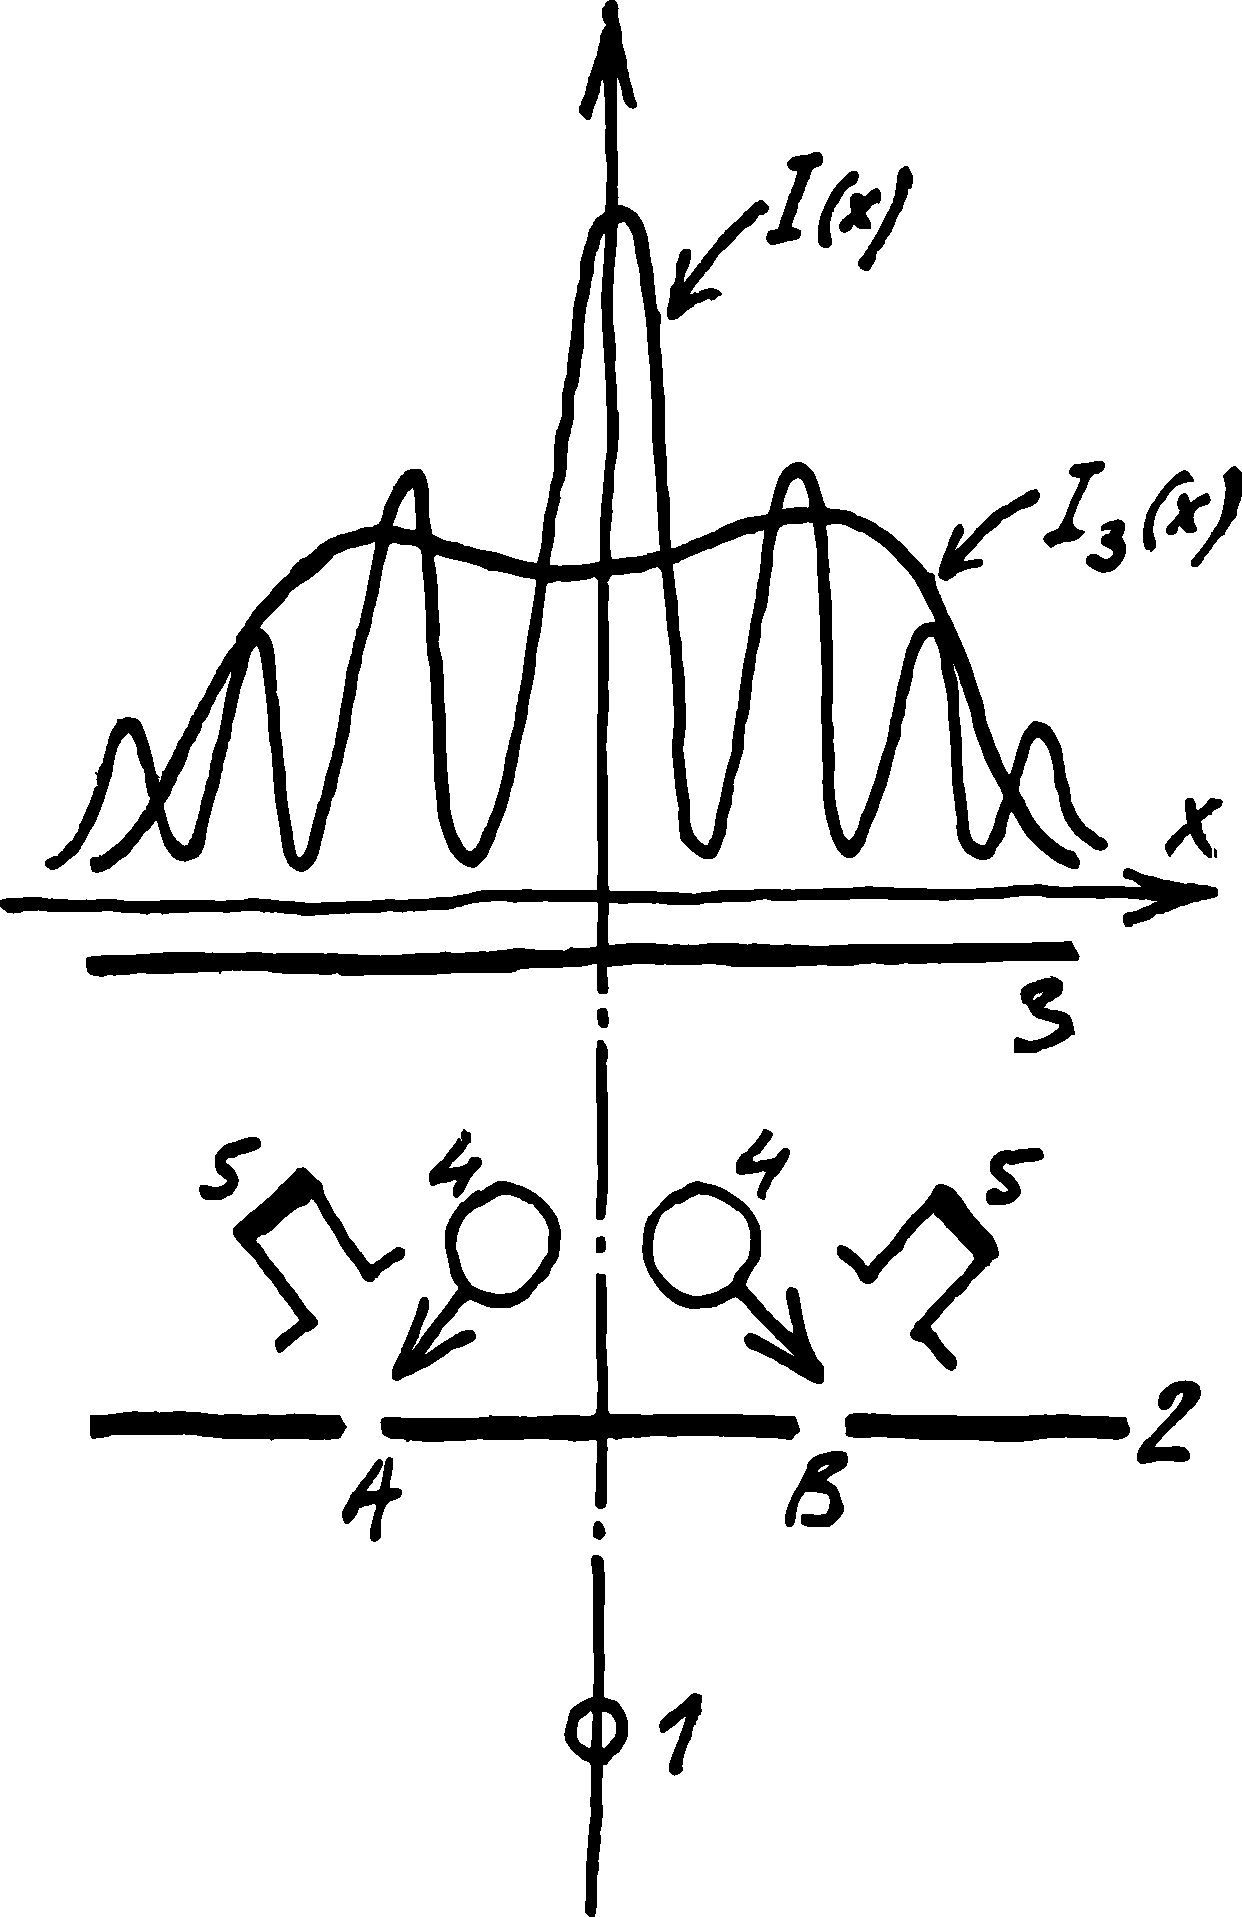
\includegraphics[width=\textwidth]{figures/fig-07-03.pdf}
\caption{Observing the microparticle in a double slit experiment.}
\label{fig-7.3}
\end{marginfigure}


So, we place an electron source at point \textsf{1}, switch on the light sources \textsf{4} and watch the photodetectors \textsf{5}.
We shall assume that the electrons pass through the apparatus one by one: the source emits an electron only after the preceding one has reached the detector screen. What does the experiment show? It always turns out that only one photodetector (either left or right) is activated and both photodetectors are never activated simultaneously. It means that the electron passes not through two slits but only through one, Moreover, we can always indicate the slit through which any electron passes.


The reader may surmise that to explain interference we again have to start talking about an electron ``perceiving'' the neighbouring slit by some secret means, while passing through a slit. We shall not jump to conclusions but shall first carry out the experiment to the end; we obtain a sufficiently large number of events of electron incidence on the detector screen \textsf{3} and see how they are distributed. Here, we get a surprise. On screen \textsf{3} we get not the interference curve $I(x)$ but the additive curve $I_{3}(x)$.


We repeat the experiment after switching off the light sources (thus depriving ourselves of the possibility of ``observing'' the passage of the electrons through the slits). In this case we again observe the interference curve $I(x)$.


The situation is such that interference occurs when light sources are switched off and is absent when they are switched on. As soon as we try to control the process of passage of electrons through two open slits, the interference disappears. In other words, our observation of the behaviour of electrons near the slits destroys the interference!


A change in the nature of the motion of electrons upon the switching on of the light sources has a simple physical explanation: this change is the result of collision of photons with the electrons ``being controlled'' In the process of measurement some influence on the object under investigation is inevitable. Here only one thing is important -- can this influence be made sufficiently
small? Maybe the experiment considered above was too crude? Maybe we should somehow try to observe the electrons more delicately, so that the interference picture is not destroyed by this. 

But how to reduce the influence of a photon on an electron? It is obvious that a reduction in the light intensity of the sources would not yield anything -- light intensity is associated with the number of photons in a beam, thus a reduction in the intensity will simply result in an increase in the number of ``unregistered'' electrons. We must reduce the energy of a single photon. But for this we shall have to increase the wavelength of the radiation and this will lead to an increase in the spatial delocalization of the photon (a photon is localized in space with an accuracy not exceeding its wavelength) and thus for a wavelength exceeding the distance between the slits the photon will no longer be in a position to register a particular slit.


\begin{marginfigure}[1cm]
\centering
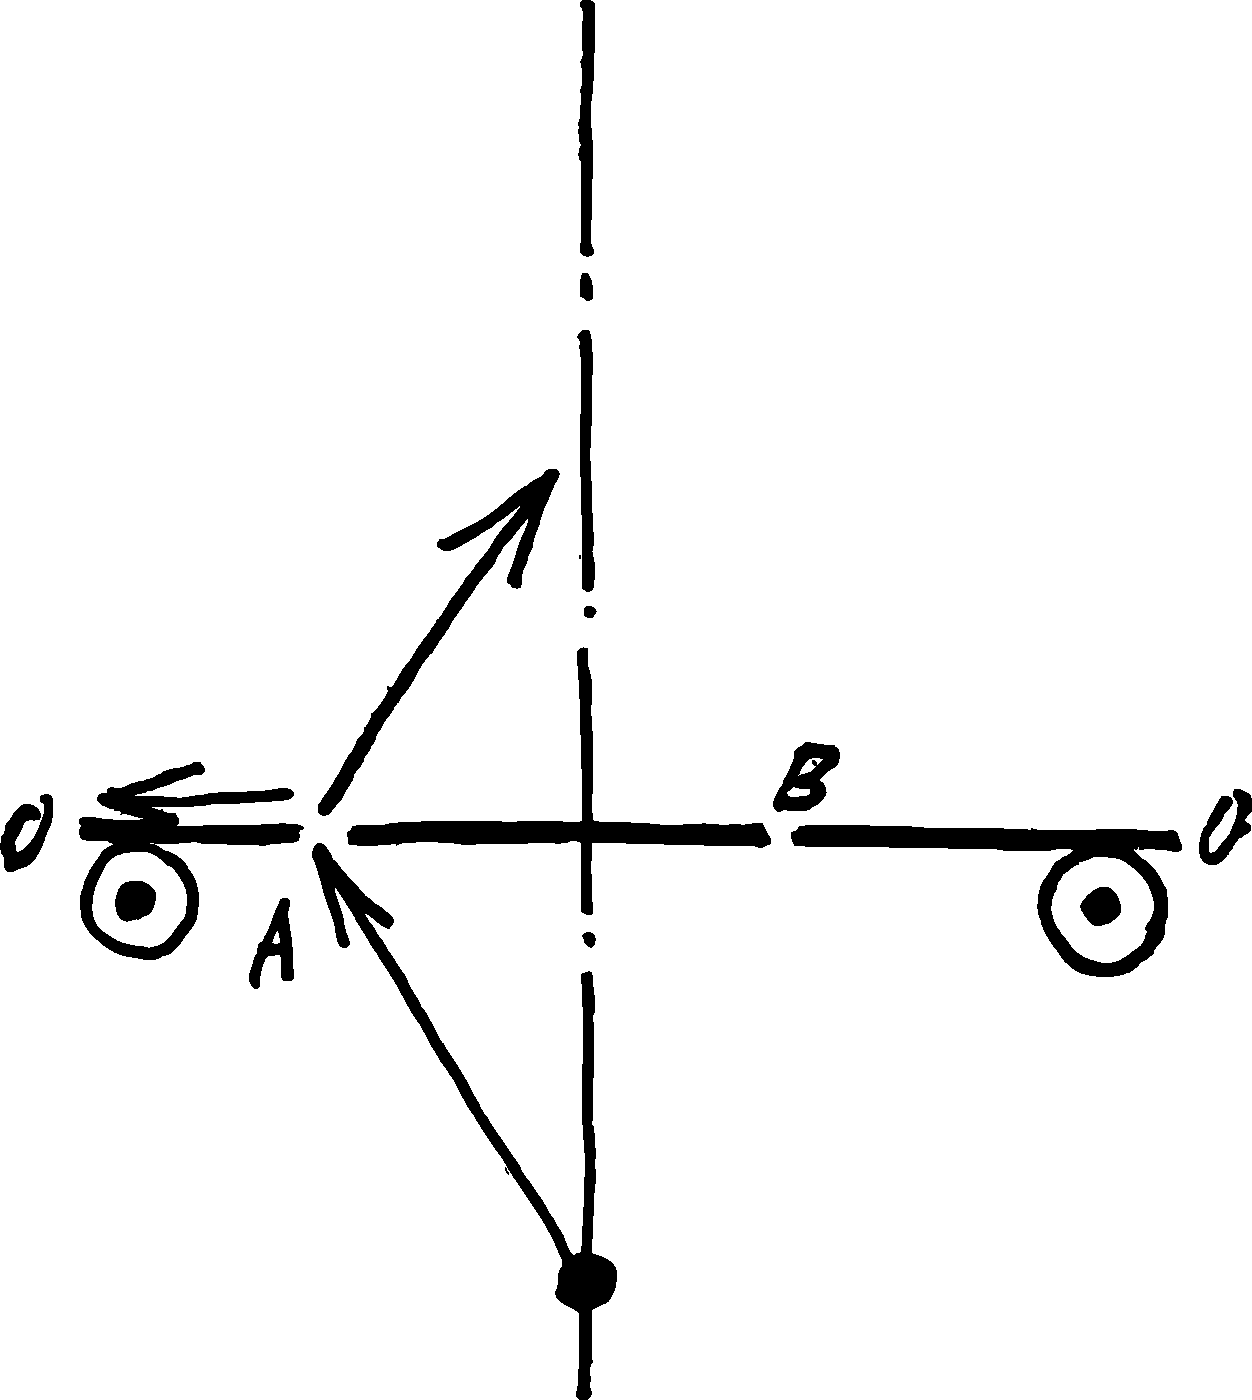
\includegraphics[width=\textwidth]{figures/fig-07-04.pdf}
\caption{Modifications to the double slit experiment.}
\label{fig-7.4}
\end{marginfigure}

But, may be, we could think of some other experiment -- without resorting to the scattering of photons by electrons? For example, isn't it possible to try to construct an extremely light screen with slits in such a way, that it could move to the left or right upon being struck by individual electrons? The screen deflects to the left if an electron passes through the left slit and to the right if it passes through the right slit (\hyperref[fig-7.4]{Figure \ref{fig-7.4}}). But if the electron passes through two slits simultaneously, the screen will not move at all. Thus, we just have to follow the movement of the screen. It would appear that at least in principle the aim has been achieved -- the required delicate experiment has been conceived. But it is meaningless to set up such an experiment. To make sure that this is so, we recall the uncertainty relation for momentum and coordinate. It follows from this relation that if the experimental conditions really permit us to register the momentum of the screen due to a recoil from the electron impingement, the same condition must lead to an uncertainty in the position of the screen on the line $OO$ (\hyperref[fig-7.4]{Figure \ref{fig-7.4}}). Consequently, the shift in such a screen does not permit one to draw any conclusion on the nature of passage of an electron through the slits. If, on the other hand, we fix the position of the screen on the line $OO$, then it is easy to see that a measurement of the momentum of its recoil will become impossible.


Several attempts were made to devise such an experiment in which the passage of electrons through a screen with slits could be ``controlled'' without seriously influencing the electrons themselves (so that the interference is not destroyed). But all these attempts proved futile. As a result, we must admit that the above conclusion regarding the destruction of interference caused by observing the behaviour of electrons near the slit, is of a fundamental nature. In other words, the effect of observation (measurement) destroying interference cannot be eliminated in principle.

\clearpage

\textsf{\Large \textcolor{darkgray}{A Brief Interlude}}

%\label{interlude-03}
\vspace*{10pt}
\begin{verse}
\texttt{\small
He was going into one room \\
And by mistake entered another \ldots \\[5pt]
Griboiedoff (\emph{Gore ot Ouma})}
\end{verse}

\textsc{Reader}: This means we were not able to determine exactly how an electron passes through a screen with slits-through one slit or simultaneously through both the slits?
\\
\textsc{Author}: Indeed, we couldn't.
\\
\textsc{Reader}: But then experiment 2 did not attain its goal. Was it necessary to consider it?
\\
\textsc{Author}: Yes, it was. The experiment did not answer the question posed by us. So what? It just means that the question was not formulated properly. We see that we cannot question all the phenomena of nature. 
\\
\textsc{Reader}: Does the whole idea of the experiment lie in its negative result? 
\\
\textsc{Author}: This is not to be ignored. However, as we shall see later, it also contains a positive result of utmost importance. In fact, we were looking for one thing, but we found another.
\\
\textsc{Reader}: And what is that?
\\
\textsc{Author} Let us not make haste. We shall first consider our system e fundamental experiments to the end.\\[10pt]

Let \marginnote{Experiment 3 (Passage of Photons Through Polarizers)
} us pass a beam of light through a polarizer, say, a tourmaline crystal. A \emph{linearly polarized} light beam emerges from the crystal. The direction of polarization of the beam is determined by the orientation of the polarizer with respect to the beam (the direction of polarization coincides with the direction of the axis of the polarizer). Let us denote the intensity of the linearly polarized light beam through $I$. 


Further, we place a second polarizer in the path of the linearly polarized light beam and consider the following three cases: 
\begin{enumerate}[label=(\alph*), leftmargin=1cm]
\item the axis of the second polarizer is parallel to the axis of the first; 
\item the axis of the second polarizer is perpendicular to the axis of the first; 
\item the axis of the second polarizer makes an angle a with the axis of the first. 
\end{enumerate}

We shall measure the intensity of light emerging from the second polarizer. In case (a) we get intensity $I$, in case (b) we do not get anything, while in case (c) we get a light beam of intensity $I \cos^{2} \alpha $, polarized along the axis of the second polarizer. These cases are shown in \hyperref[fig-7.5]{Figure \ref{fig-7.5}}, where $AA$ and $BB$ are the directions of the axis of the first and the second polarizers, respectively. 


The above experiment is well known in classical optics. However, like the Young experiment on interference, it has a direct relation to quantum mechanics. As in the case of interference we shall reduce the intensity of the light beam till the photons pass one by one through our set-up. We shall consider the cases illustrated in \hyperref[fig-7.5]{Figure \ref{fig-7.5}} as applied to single photons. 

\begin{marginfigure}[1cm]
\centering
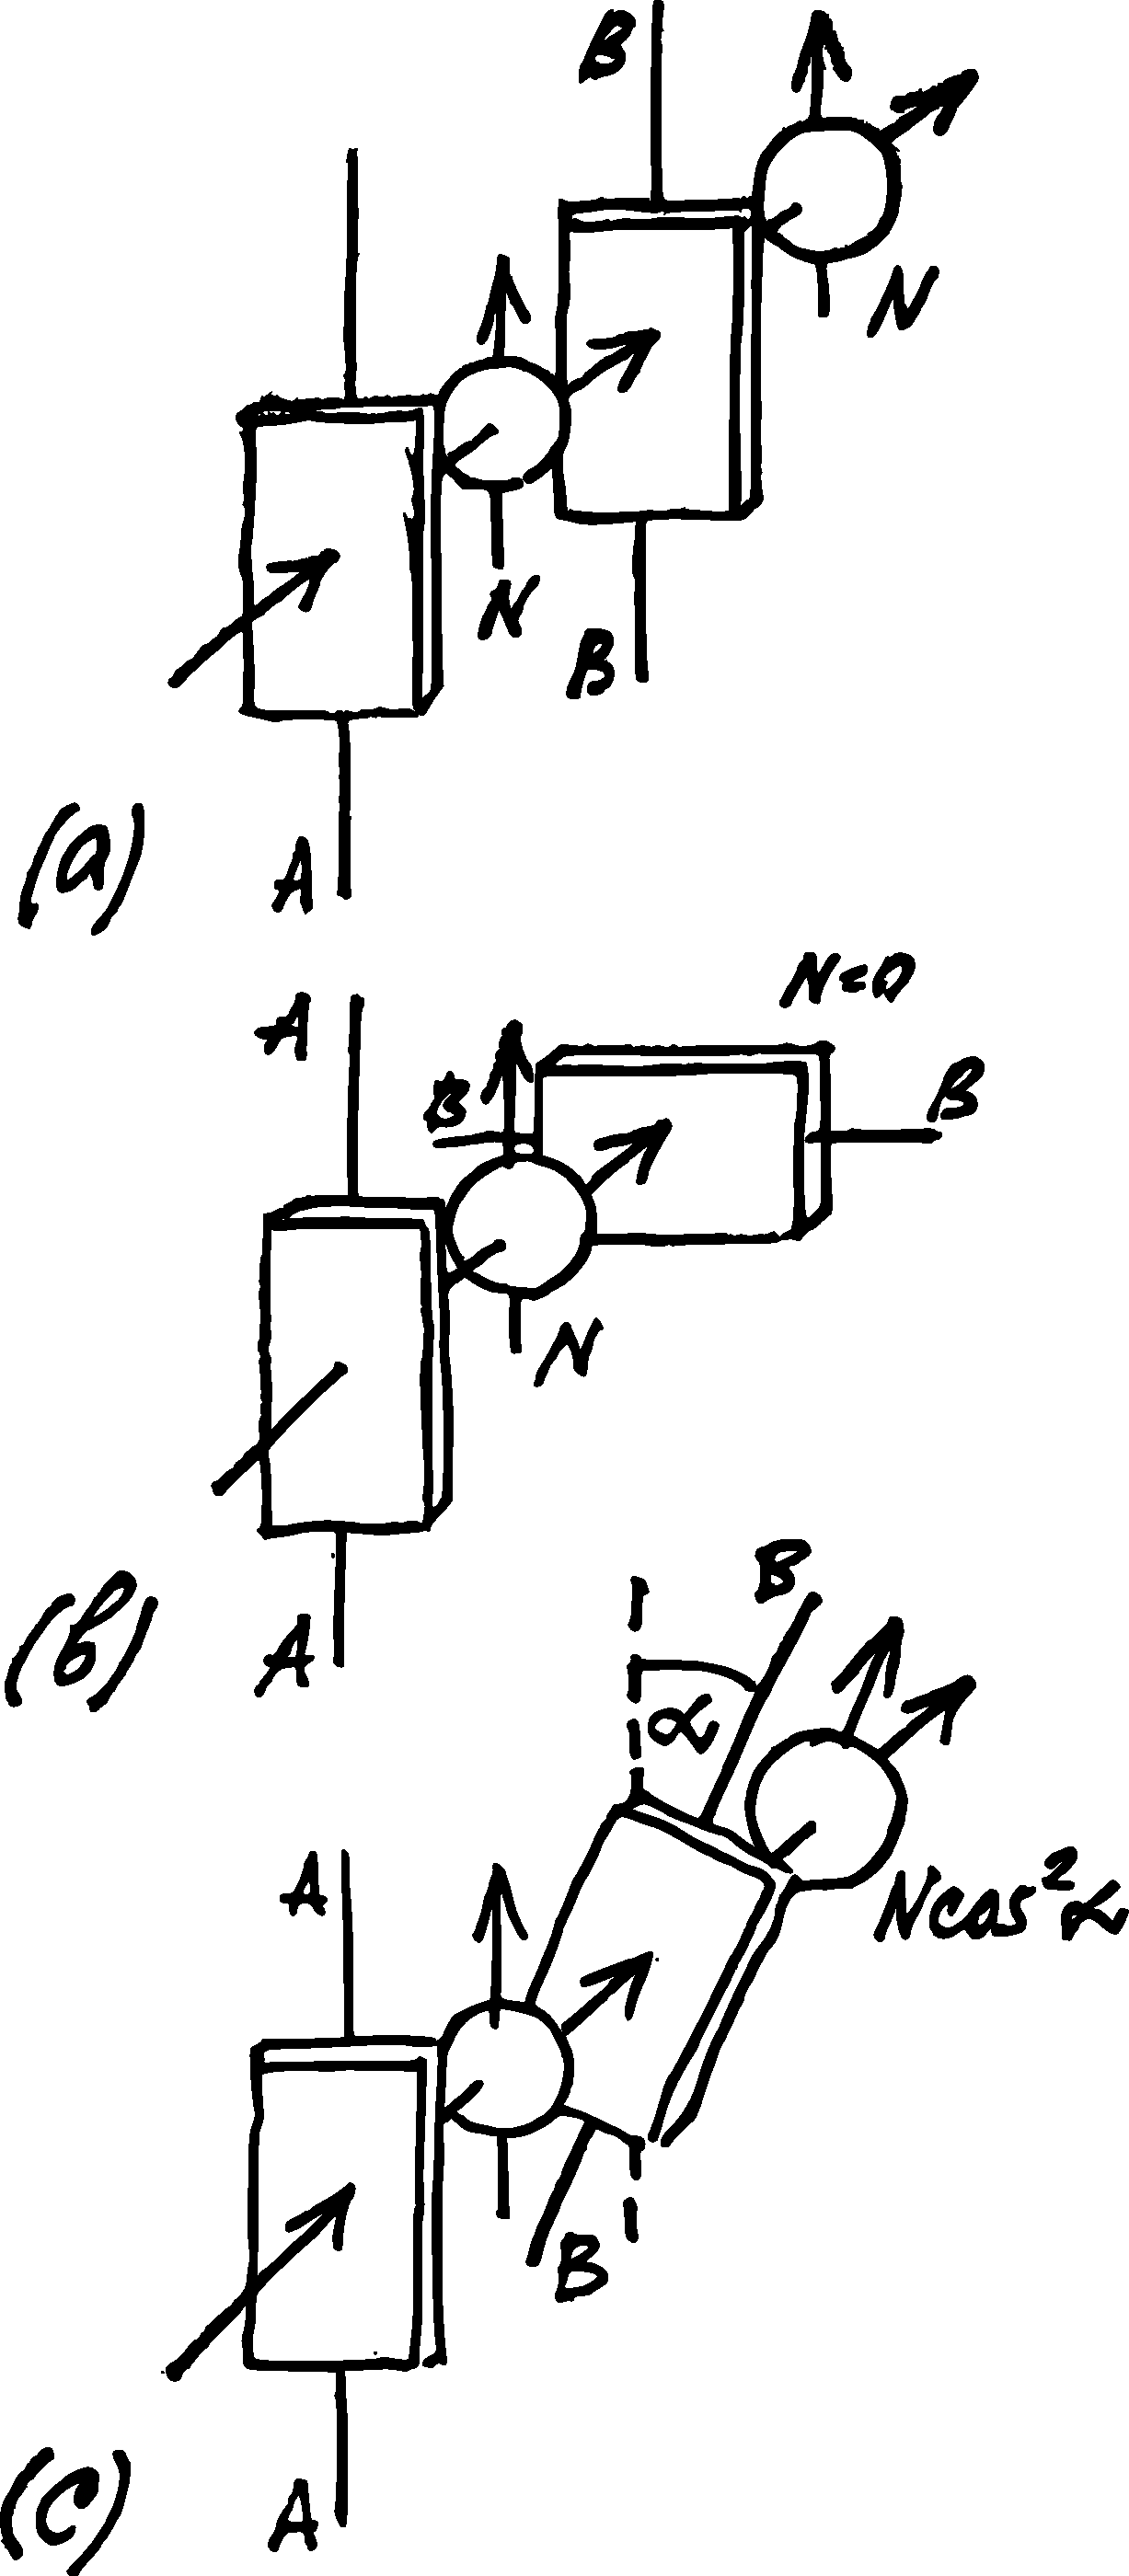
\includegraphics[width=\textwidth]{figures/fig-07-05.pdf}
\caption{Passage of photons through two polarizers.}
\label{fig-7.5}
\end{marginfigure}

First of all, we recall that a photon is characterized by a definite \emph{polarization}. Moreover, this polarization corresponds to the polarization of the classical light wave from which the photon under consideration has been ``taken'' In particular, this means that after the first polarizer we shall have linearly polarized (polarized in the direction of the axis of the polarizer) photons. In the following we shall ``deal'' only with these photons and shall call them ``initial photons''


In case (a) the initial photon always passes through the second polarizer; in case; (b), on the contrary, it never passes the second polarizer. These results are not unexpected. But what happens in case (c)? It turns out that in this case the photon may pass through the second polarizer or it may not. Moreover, it is absolutely impossible to predict which of the two alternatives (passing or not passing) will be realized for a given initial photon. If it so happens that the photon passes through the second polarizer, its polarization will change -- it will be polarized in the direction of the axis of the second polarizer. Thus, the fate of any particular individual photon is, in principle, unpredictable!


Let us assume further that there are $N$ initial photons. We observe their passage through the second polarizer in the case (c) and see what happens. We find that if $N$ is sufficiently large, the number of photons passed can be predicted fairly accurately; it will be about $N \cos^{2} \alpha$. In this connection, we recall our earlier remark that the unpredictability in the behaviour of an individual microparticle is related to the predictability in the behaviour of a large number of microparticles (see Experiment 1). We can say that there is a definite probability of the initial photon passing through the second polarizer. This
probability is equal to  $\cos^{2} \alpha$. 

\begin{marginfigure}[1cm]
\centering
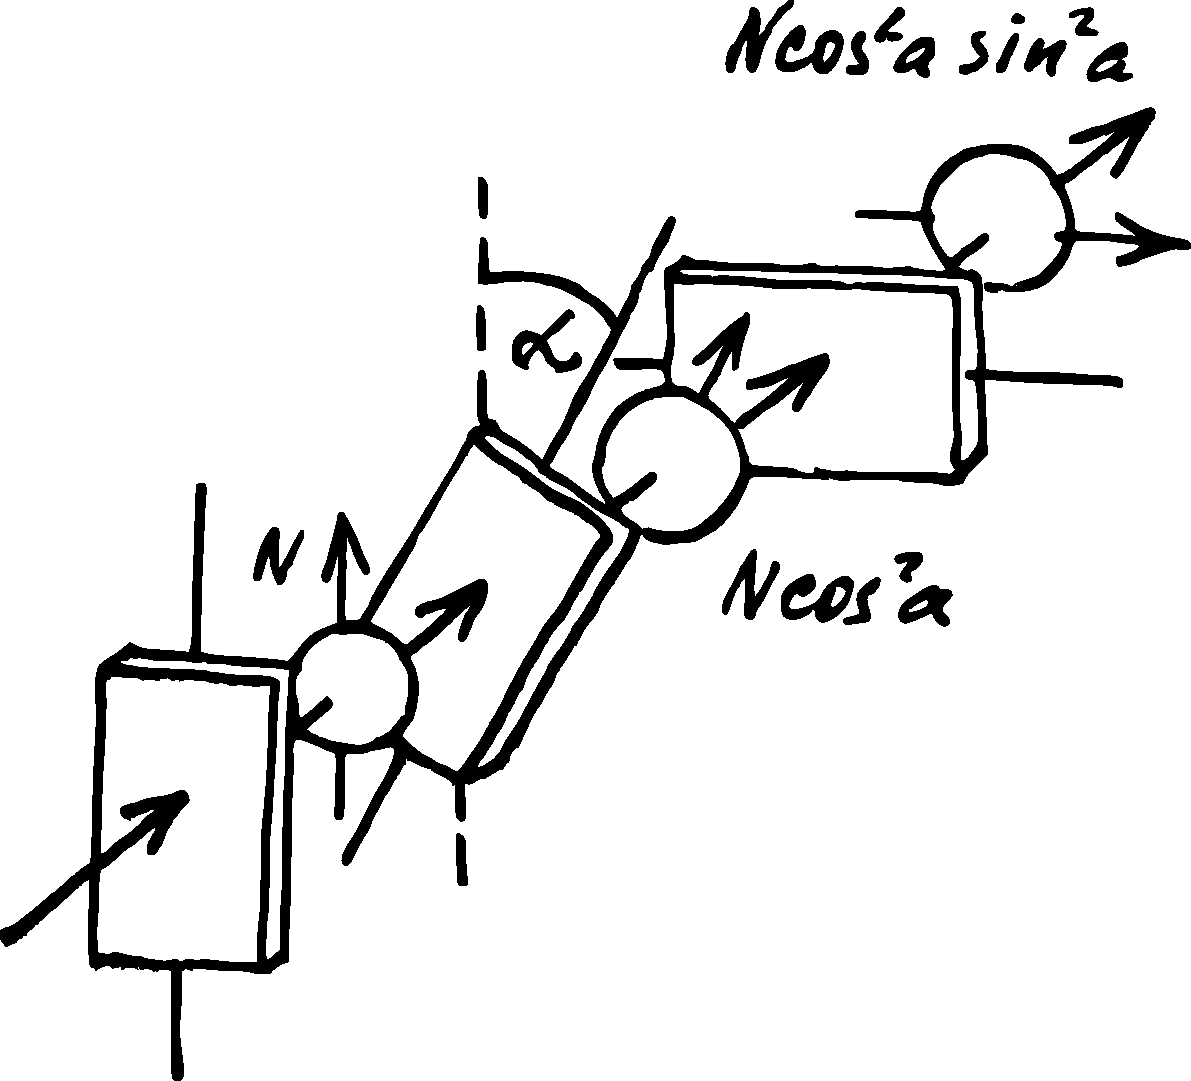
\includegraphics[width=\textwidth]{figures/fig-07-06.pdf}
\caption{Passage of photons through three polarizers.}
\label{fig-7.6}
\end{marginfigure}

Let us now complicate the experiment. We use the situation shown in \hyperref[fig-7.5]{Figure \ref{fig-7.5} (c)} and add yet another (i.e. a third) polarizer, whose axis is perpendicular to the axis of the first polarizer. The three-polarizer system under consideration is shown in \hyperref[fig-7.6]{Figure \ref{fig-7.6}}. Let $N$ be the number of initial photons (i.e. photons passing through the first polarizer). After the second polarizer, as we already know, we shall have $N \cos^{2} \alpha$ photons, the polarization of these photons coinciding with the axis of the second polarizer. Analysing further in the same way	we conclude that after the third polarizer, we must have $N \cos^{2} \alpha \sin^{2} \alpha$ photons; moreover, the polarization of these photons must
coincide with the axis of the third polarizer. The experiment certainly confirms this conclusion. 


There is nothing that appears astonishing in this (that is, of course, if we assume that our astonishment over the existence of two unpredictable possible behaviours of an individual photon has somewhat diminished). And yet there is something here which contradicts our usual concepts. Let us remove the second polarizer. Then no photons will be observed after the third polarizer. This creates a fairly interesting situation. Photons pass through this apparatus, as if they are ``filtered'' first through the second polarizer and then through the third. As a result, we at first have $N$ photons, then $N \cos^{2} \alpha$	and we are finally left with $N \cos^{2} \alpha \sin^{2} \alpha$ photons. We remove one of the ``filters'' and thus, it would appear, improve the conditions for passage of photons through the given apparatus. However, in actual practice it turns out quite differently -- now the photons do not pass through the apparatus at all!

We shall \marginnote{Experiment 4 (Scattering of Microparticles by Microparticles)} consider \emph{elastic collisions} of microparticles and use for convenience the centre of mass system for the colliding particles. \hyperref[fig-7.7]{Figure \ref{fig-7.7}} shows experimental diagram related to the system of the centre of mass of the particles. Here, $A$ and $B$ are particle beams, \textsf{1} and \textsf{2} are the counters for scattered particles, deployed on the line perpendicular to the direction of motion of the particles before collision. Thus, we consider here the scattering of particles through an angle of \ang{90} in the centre of mass system. We note that the picture of the process in the centre of mass system may considerably differ from the analogous picture in the laboratory system. Thus, for example, in the laboratory system the counters \textsf{1} and \textsf{2} may not be on the same line. Besides, in actual practice only one beam of particles -- (for example, particles of type $A$) may be used while the particles of the other type (type $B$) constitute the stationary target. It is assumed that every time the experiment in the laboratory system is conducted in such a way that the diagram shown in \hyperref[fig-7.7]{Figure \ref{fig-7.7}} is applicable for the centre of mass system of the particles.

\begin{marginfigure}%[4cm]
\centering
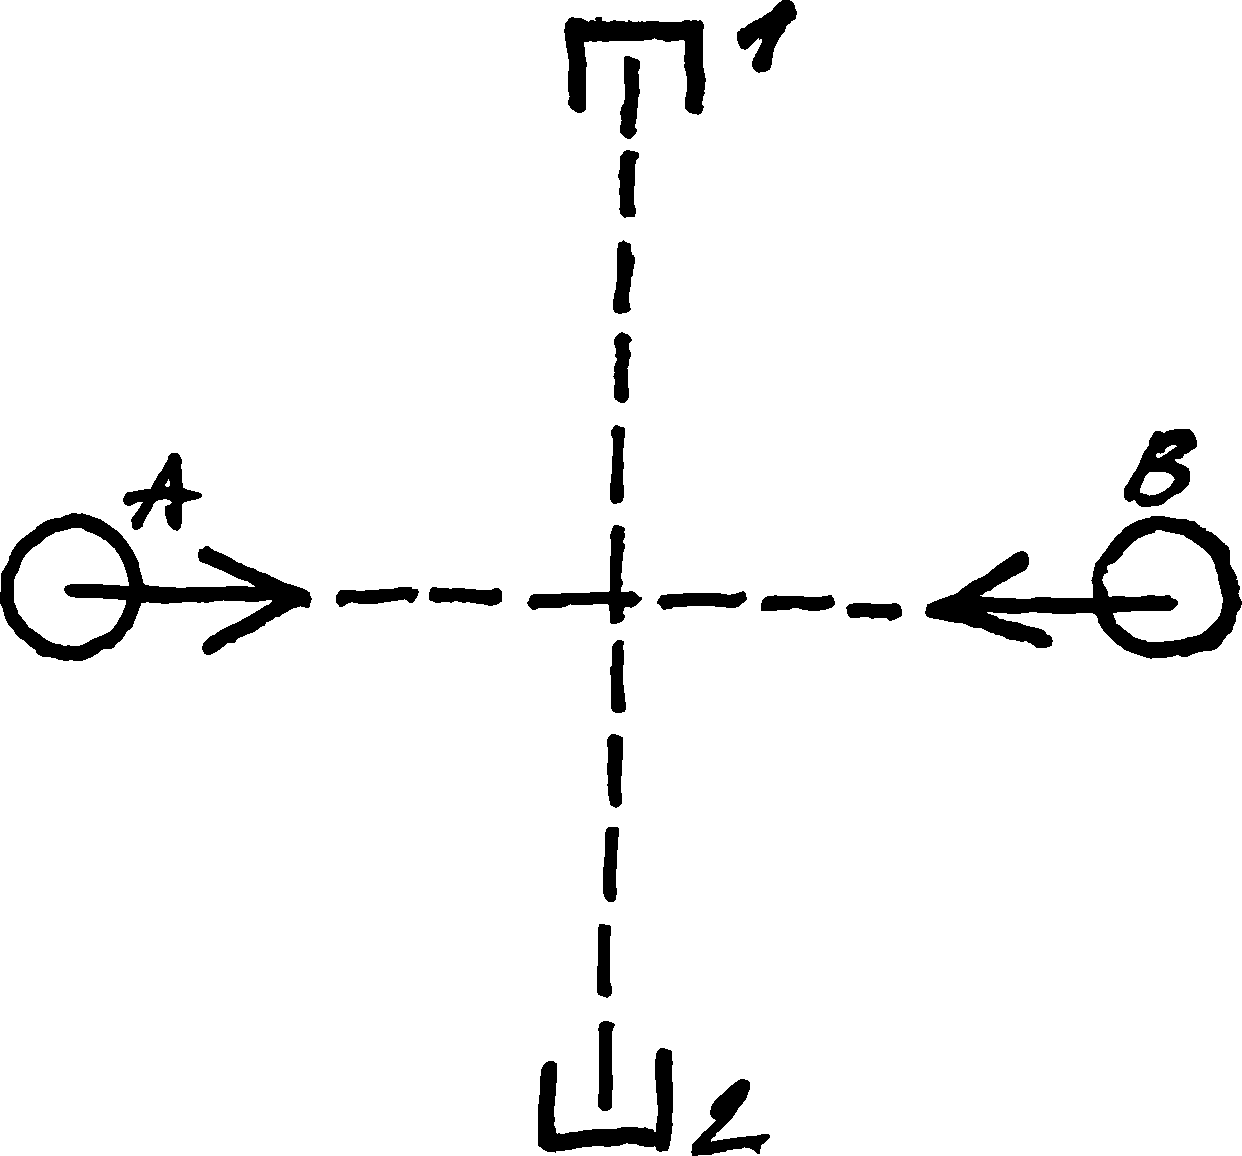
\includegraphics[width=0.8\textwidth,angle=2]{figures/fig-07-07.pdf}
\caption{Elastic collision of microparticles.}
\label{fig-7.7}
\end{marginfigure}

We shall consider different examples as applied to the above diagram, measuring each time the probability of scattering of particles by the number of simultaneous activations of counters \textsf{1} and \textsf{2}.

\begin{description}[font=\bfseries, leftmargin=1cm]
\item[First Example.] Particles of type $A$ are $\alpha$-particles
  ($^{4}$He nuclei), particles of type Bare $^{3}$He nuclei; counter
  \textsf{1} registers only $\alpha$-particles, counter \textsf{2},
  only $^{3}$He nuclei. Let $w$ be the probability of scattering
  measured in this case.

\item[Second example.] The particles are the same, but now each
  counter can register both $\alpha$-particles and $^{3}$He nuclei. In
  this case the measured probability of scattering turns out to be
  $2w$. This result appears quite natural -- the doubling of the probability $w$ is associated with the realization of the two alternatives shown in \hyperref[fig-7.8]{Figure \ref{fig-7.8}}.

\begin{marginfigure}%[4cm]
\centering
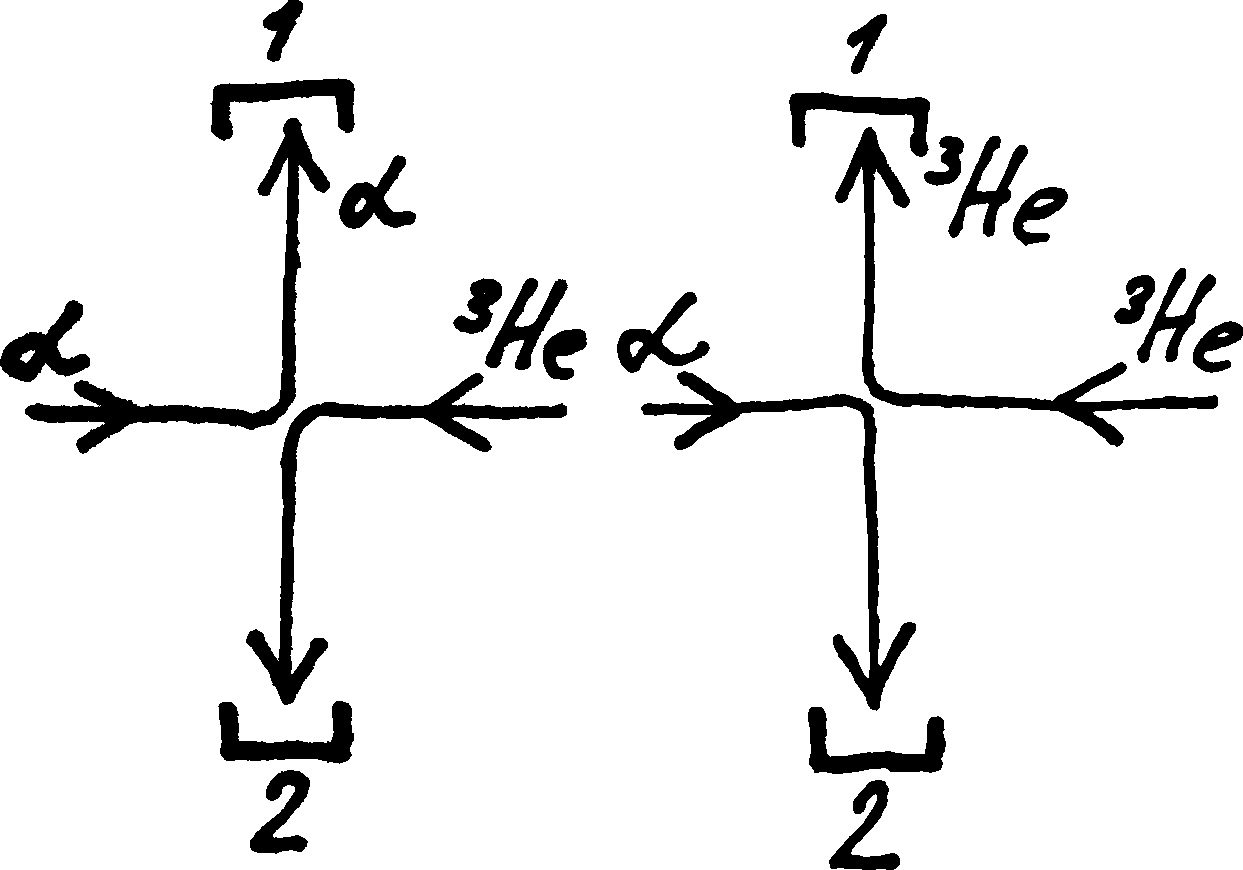
\includegraphics[width=\textwidth]{figures/fig-07-08.pdf}
\caption{Elastic collision of microparticles.}
\label{fig-7.8}
\end{marginfigure}

\item[Third example.] We replace $^{3}$He nuclei by
  $\alpha$-particles. Let the $\alpha$-particles be scattered now by
  $\alpha$-particles. It would appear that in this case the scattering
  probability must be the same (or nearly the same) as in the previous
  case, i.e. $2w$. The experiment, however, yields quite a different
  result, $4w$. A ``mere'' replacement of $^{3}$He nuclei by $^{4}$He
  nuclei has doubled the scattering probability! Still more unexpected
  results are observed by taking into account the spin states of the
  colliding particles (in the case of $\alpha$-particles the question
  of taking spin into account did not arise since $\alpha$-particles
  do not have spin). In this connection let us consider scattering of
  electrons by electrons. We recall that an electron may exist in two
  spin states $ \left( \sigma = \nicefrac{1}{2}, \; -\nicefrac{1}{2}
  \right) $. Electrons created as a result of photoelectric emission,
  for example, appear in one spin state or the other with same
  probability. Such electron beams are termed nonpolarized; half the
  electrons in them have $\sigma = \nicefrac{1}{2}$ and the other
  half, $\sigma = - \nicefrac{1}{2}$ . If we take special measures, we
  may obtain a polarized electron beam in which all electrons are in
  the same spin state. Having made these remarks, let us now return to
  the diagram in \hyperref[fig-7.7]{Figure \ref{fig-7.7}} and continue
  the list of examples under consideration. Moreover, we shall assume
  that the energies of the colliding particles are considerably small,
  hence, the possibility of an electron changing its spin state upon
  collision need not be taken into consideration.


\item[Fourth example.] The two electron beams are nonpolarized. Let the scattering probability measured in this case be $w_{e}$. 


\item[Fifth example.] The electron beams are polarized but in both
  directions. For example, $A$-electrons have spin $\sigma =
  \nicefrac{1}{2}$ and $B$-electrons, $\sigma = - \nicefrac{1}{2}$. In
  this case the scattering probability turns out to be $2w_{e}$.


\item[Sixth example.] The electron beams are polarized in the same
  direction. In this case the counters \textsf{1} and \textsf{2} are
  ``silent'' -- the scattering probability is zero! 
\end{description}
As will be seen later, the results of experiments on the scattering of microparticles reveal fundamental quantum-mechanical laws.


We \marginnote{Conclusion} have thus considered a system of four fairly simple experiments. While considering them we emphasized the unexpectedness of the results, which indicates the impossibility of their classical explanation. The system of basic experiments could have been enlarged and supplemented by more complex experiments. However, we shall not do this. We content ourselves with considering the four experiments, as we think that all the basic principles of quantum mechanics are fairly clearly revealed in them. On the basis of the experiments considered, we move on to build up in the following sections a system of quantum- mechanical concepts which essentially expresses the physical foundations of quantum mechanics.

\section{Amplitudes of Transition Probabilities (Formulation of Basic Principles)}
\label{sec-08}

We \marginnote{Introduction to the Concept of Amplitude of Transition
  Probability} suppose that for a certain microparticle definite
\emph{initial} and \emph{final} states ($s$-state and $f$-state,
respectively) are considered. The specific characteristics of these
states as well as the nature of the microparticle are immaterial for
the present. As has been pointed out earlier, the transition of the
microparticle between the two given states has, as a rule, a
\emph{probabilistic} character. We therefore introduce into the
picture the \emph{transition probability} $w_{s \to f}$. In quantum
mechanics, apart from transition probability, the concept of the
\emph{amplitude of the transition probability} $\Braket{f|s}$
\sidenote{The treatment of quantum mechanics on the basis of
  probability amplitudes is given in books by Feynman [3-5J and Dirac
  [9).} is also introduced. Generally speaking, it is a complex
number, the square of whose modulus is equal to the transition
probability:
\begin{equation}%
w_{s \to f} = |\Braket{f|s}|^{2}	
\label{eq-8.1}
\end{equation}
Note that the amplitude of the transition probability is written so that the initial state is on the right and the final one on the left (as if it were read from right to left). Henceforth for brevity we shall call the amplitude of the transition probability the transition amplitude (and sometimes even more briefly simply the amplitude).

Besides introducing the concept of the transition amplitude, which is
of utmost importance to quantum mechanics, we shall devote this
section to a formulation of a number of basic principles in their most
general form. The reader should not be perplexed over the formality of
the exposition in this section. It will be compensated for in the next
section where we shall demonstrate the principles indicated in this
section using specific examples. Moreover, among other things, we
shall consider the connection between these principles and the
experiments discussed in \hyperref[sec-07]{Section~\ref{sec-07}}. This
will provide, on one hand, grounds for the formal description of the
principles and, on the other hand, an explanation of the astonishing
experimental results.


We \marginnote{Basic Rules of Working with Amplitudes}shall indicate four basic rules of working with transition amplitudes. These rules should be considered as postulates forming the basis of a system of quantum-mechanical concept which are in conformity with experiment.
\begin{marginfigure}[2cm]
\centering
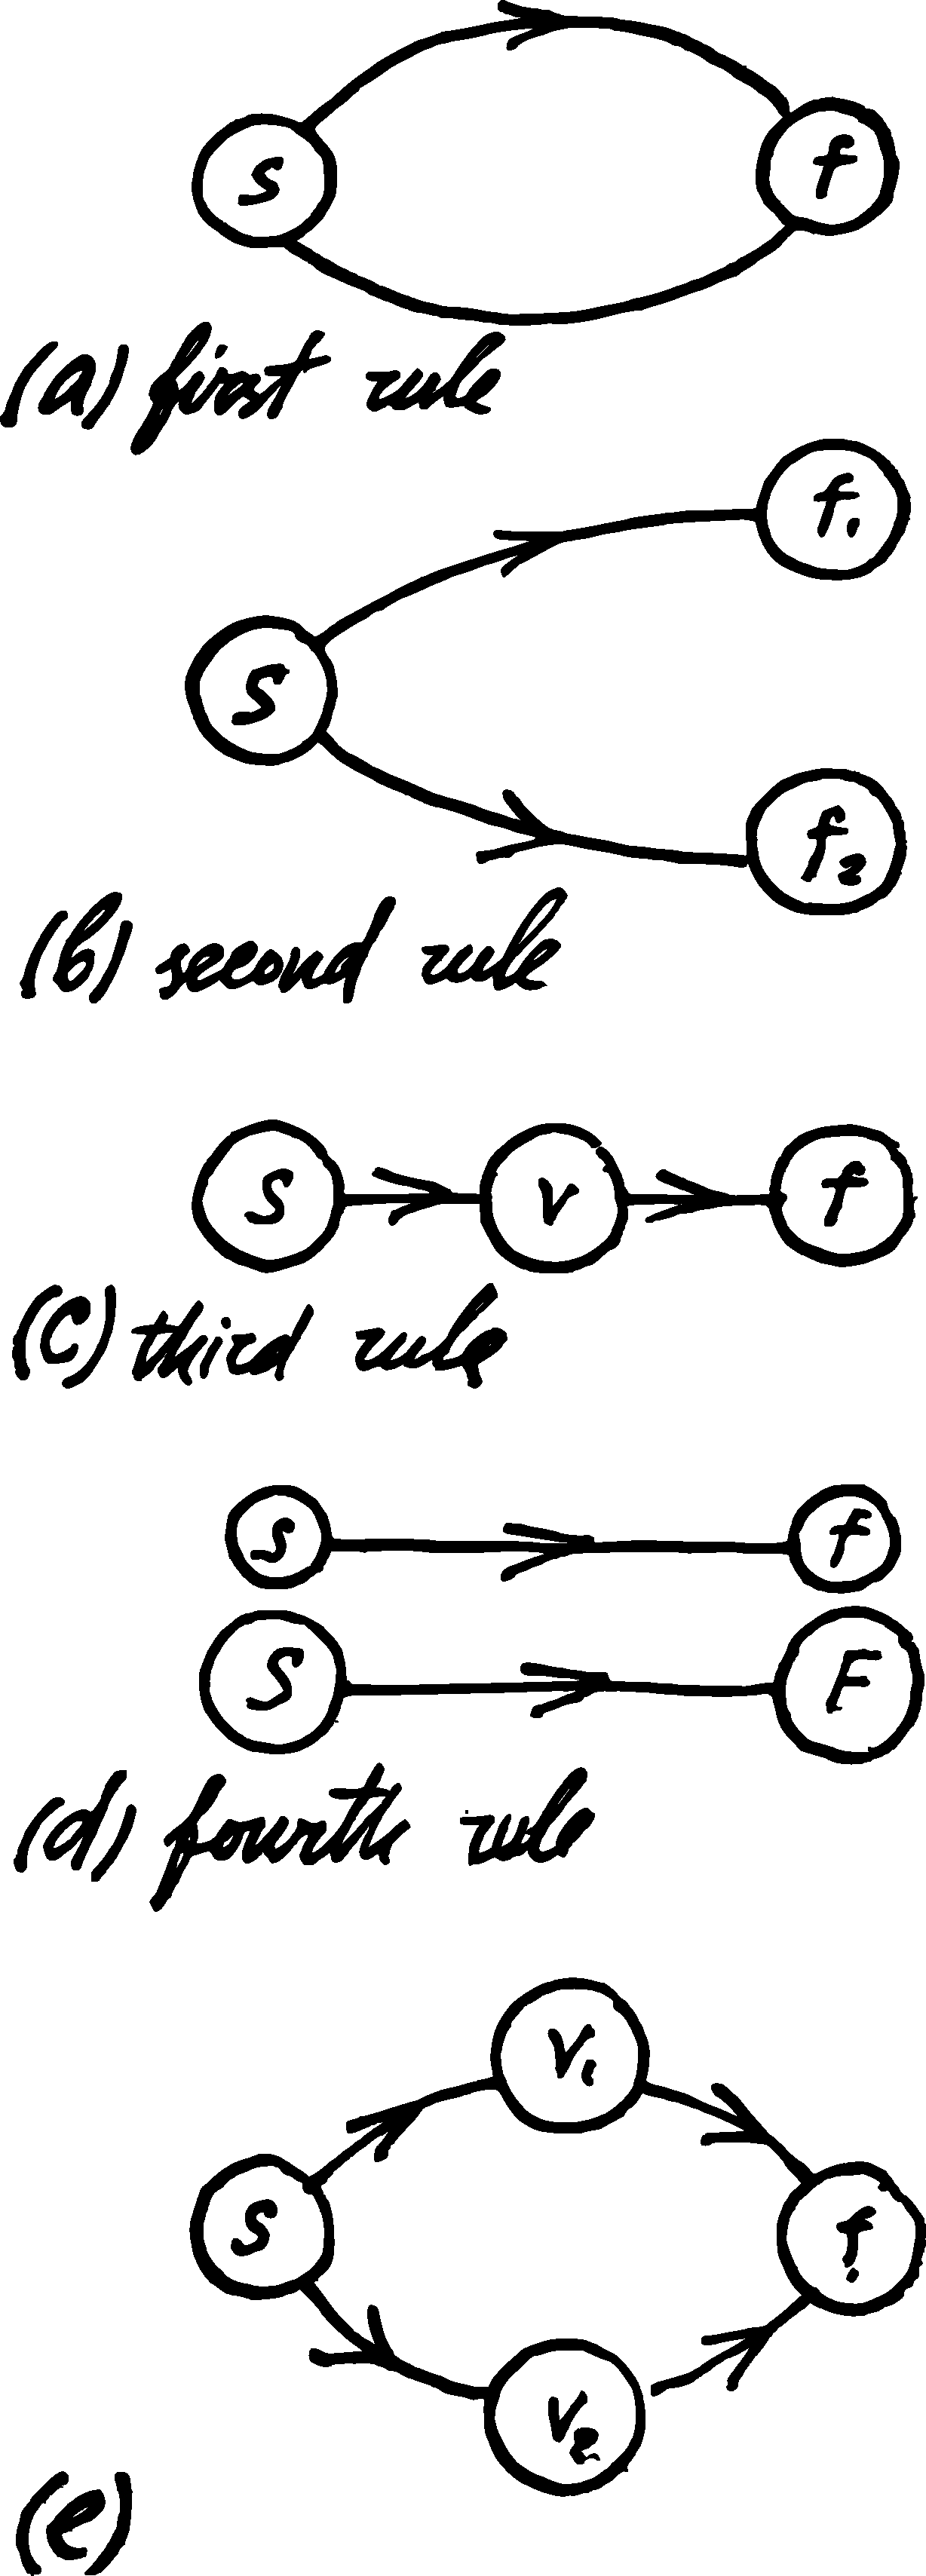
\includegraphics[width=\textwidth]{figures/fig-08-01.pdf}
\caption{Rules of working with amplitudes.}
\label{fig-8.1}
\end{marginfigure}

\begin{description}[font=\bfseries, leftmargin=1cm]
\item[First Rule.] We assume (\hyperref[fig-8.1]{Figure \ref{fig-8.1}(a)})
  that there are several \emph{physically indistinguishable} ways
  (paths) in which a microparticle can move from $s$-state to
  $f$-state. In this case, the resulting transition amplitude is the
  sum of the amplitudes corresponding to the different modes of
  transition:
\begin{equation}%
\Braket{f |s} = \sum_{i} \Braket{f|s}_{i}	
\label{eq-8.2} 
\end{equation}
(the index $i$ denotes the $i$-th mode of transition). 

\item[Second Rule.] We assume (\hyperref[fig-8.1]{Figure
    \ref{fig-8.1}(b)})that there are several final states $(f_{1}, f_{2},
 \ldots , f_{i}, \ldots)$ and that we are considering the probability
 of transition to any of these states, no matter which state it is. In
 this case, the resulting transition probability  $|\Braket{f|s}|^{2}$
 is the \emph{sum of the transition probabilities} to the various
 final states:
\begin{equation}%
|\Braket{f |s}|^{2} = \sum_{i} \Braket{f|s}_{i}	
\label{eq-8.3} 
\end{equation}

\item[Third Rule.] Let us assume (\hyperref[fig-8.1]{Figure
    \ref{fig-8.1}(c)}) that the transition $s \to f$ takes place
  through some intermediate state ($v$-state). In this case we
  introduce the idea of the amplitude of the successive transitions $s
  \to v$ and $v \to f$ (corresponding to the amplitudes $\Braket{v
    |s}$ and $\Braket{f|v}$; the resulting amplitude is the product of
  these amplitudes:
\begin{equation}%
\Braket{f |s} =  \Braket{f|v} \Braket{v|s}
\label{eq-8.4} 
\end{equation}

In other words, if the transition is broken up into successive steps,
the transition amplitude is expressed by the product of the amplitudes
of the separate steps. It should be noted that if the notation in
(\ref{eq-8.4}) is read from right to left, then the states will be designated
in proper sequence: first the initial state, followed by the
intermediate state and then the final state.


\item[Fourth Rule.] Suppose (\hyperref[fig-8.1]{Figure
    \ref{fig-8.1}(d)}) have two independent microparticles. Suppose
  one microparticle undergoes a transition $s \to f$ and the other
  simultaneously undergoes a transition $S \to F$. In this case the
  resulting transition amplitude for the system of microparticles is
  given by the product of the transition amplitudes for the individual
  micropartlcles: 
\begin{equation}%
\Braket{fF |sS} =  \Braket{f|s} \Braket{F|S}
\label{eq-8.5} 
\end{equation}

\end{description}

We can see that the second, third and fourth rules appear quite
natural since, together with (8.1), they represent well-known
theorems, i.e. the theorem of addition of probabilities (second rule)
and the theorem of multiplication of probabilities of independent
events (third and fourth rules). Only the first rule, which may be
called the \emph{rule of addition of amplitudes}, appears unusual. In
a certain sense, the entire system of quantum-mechanical concepts is
based on the rule of the addition of amplitudes. 

Suppose \marginnote{Distinguishable and Indistinguishable
  Alternatives. Interference of Amplitudes } that the transition of a
microparticle from the initial to the final state ($s \to f$
transition) always takes place through one of the intermediate states
$(v_{1}, v_{2}, \ldots v_{i} \ldots)$ (\hyperref[fig-8.1]{Figure
  \ref{fig-8.1}(e)}) this case, one or the other mode of transition $s
\to f$ (one alternative or the other) is determined by the
``participation'' of the corresponding intermediate state in the
transition.

We take two different cases. Suppose in the first case the
intermediate state through which a given transition takes place is
known. This is the case of physically distinguishable alternatives. To
describe this we must combine the second and the third rules. The
transition probability that we obtain as a result will be of the form

\begin{equation}%
|\Braket{f |s}|^{2} =  \sum_{i} |\Braket{f|v_{i}} \Braket{v_{i}|s}|^{2}
\label{eq-8.6} 
\end{equation}


One might ask: where does the second rule come in if it only involves the various final states? As a matter of fact, if we know the intermediate state at which the microparticle arrives, it may be treated as the final state of the first step of the transition. We fix the microparticle in this state and temporarily stop the experiment here. One microparticle will be fixed in one state, the others in various other states, so, a situation with different final states actually arises. We stress here that distinguishability of alternatives is connected with the actual existence of different final states (even if in the given experiment they play the role of intermediate states).


In the second case, we don't know the intermediate state through which
a particular transition takes place. This is the case of physically
indistinguishable alternatives. To describe this case we should
combine the first and the third rules. The resulting transition
probability will be of the form


\begin{equation}%
\Braket{f |s} =  \sum_{i} \Braket{f|v_{i}} \Braket{v_{i}|s}
\label{eq-8.7} 
\end{equation}

The result (\ref{eq-8.7}) is a specifically quantum-mechanical
one. When it holds, we speak of the interference of amplitudes of
transitions through different intermediate states. We emphasize that
the interference of amplitudes is possible only under conditions of
the physical indistinguishability of the alternatives corresponding to
the given experiment (the microparticle is not fixed in the
intermediate state, hence we are actually dealing only with one final
state). Changing over from amplitude in (\ref{eq-8.7}) to the
probability of transition, we get
\begin{equation}%
|\Braket{f |s}|^{2} =  \sum_{i} |\Braket{f|v_{i}} \Braket{v_{i}|s}|^{2}
\label{eq-8.8} 
\end{equation}

The difference between the cases of physically distinguishable and
indistinguishable alternatives becomes clear from a comparison of
probabilities (\ref{eq-8.6}) and (\ref{eq-8.8}). While in the first
case the probabilities of the alternatives are added, in the second
case it is the amplitudes of the probabilities of alternatives which
are added.


It \marginnote{Transition Involving Two Microparticles} is interesting
to expand somewhat the fourth rule regarding the simultaneous
transition of two microparticles, Let us suppose
(\hyperref[fig-8.2]{Figure \ref{fig-8.2}(a)}) that one microparticle
undergoes a transition $s \to f$ through the intermediate $v$-state and
that another microparticle simultaneously undergoes the transition $S
\to F$ through the intermediate $V$-state. By combining the third and
fourth rules we represent the transition amplitude for the system of
microparticles in the following form: 
\begin{equation}%
\Braket{fF |sS} =  \Braket{f|v} \Braket{v|s} \Braket{F|V} \Braket{V|S}
\label{eq-8.9} 
\end{equation}

\begin{marginfigure}[1cm]
\centering
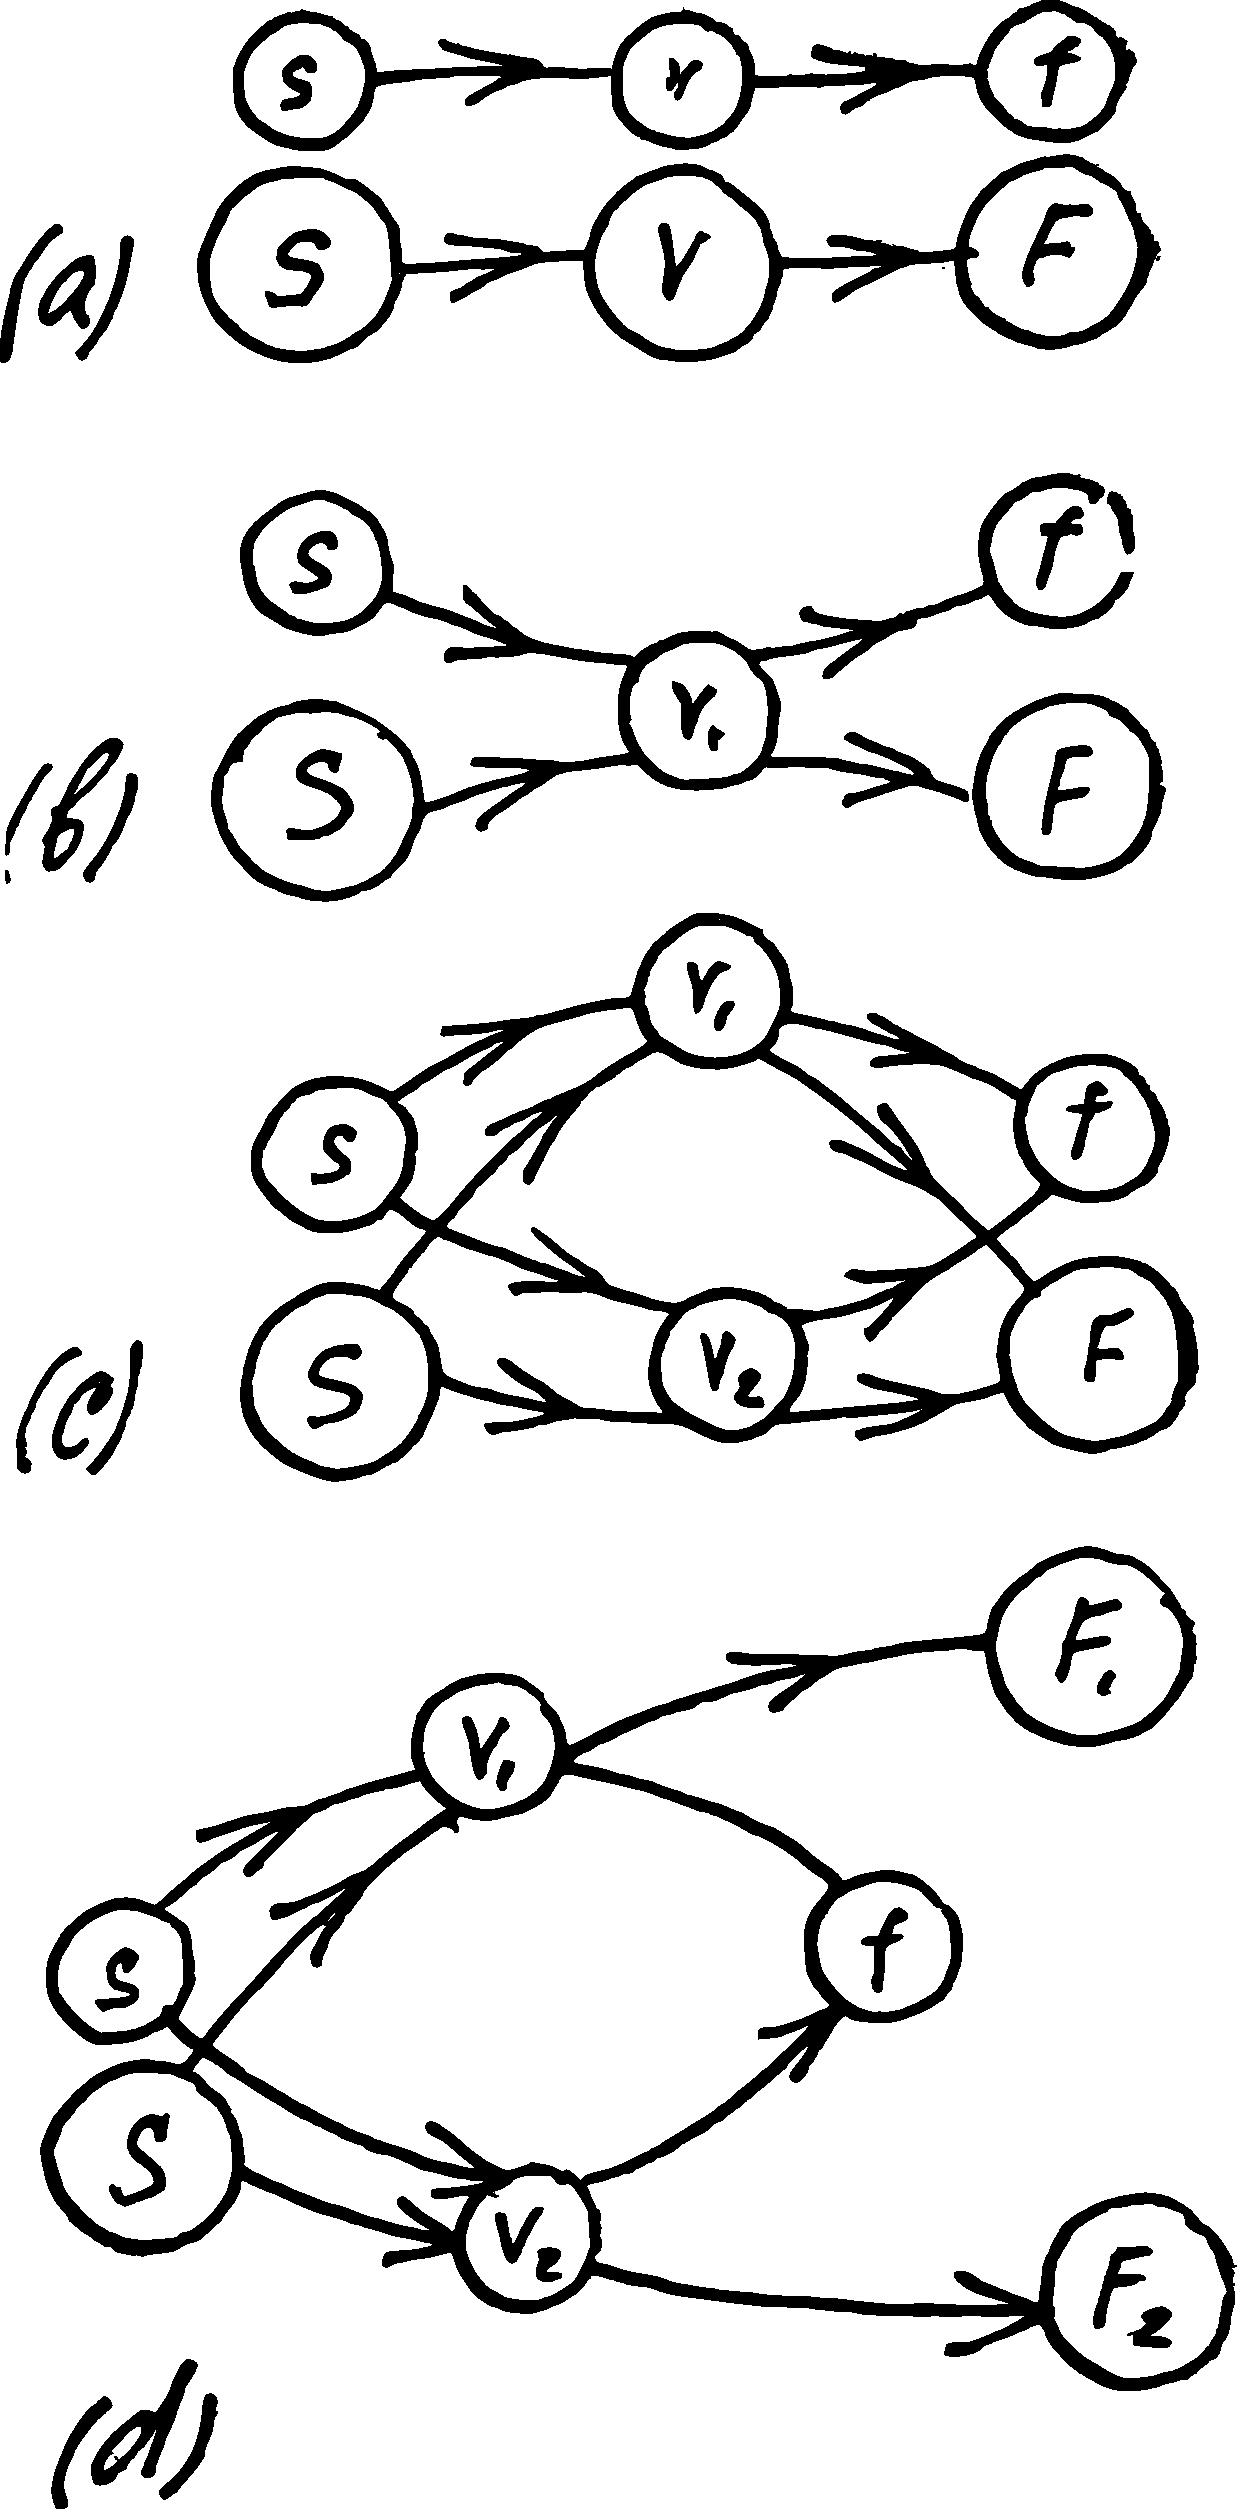
\includegraphics[width=\textwidth]{figures/fig-08-02.pdf}
\caption{Rules of working with amplitudes.}
\label{fig-8.2}
\end{marginfigure}

Let us assume further (\hyperref[fig-8.2]{Figure \ref{fig-8.2}(b)}) that both the microparticles in the process of their transitions ass through one and the same intermediate $v_{1}$-state. Then (\ref{eq-8.9}) must take the form
\begin{equation}%
\Braket{fF |sS} =  \Braket{f|v_{1}} \Braket{v_{1}|s} \Braket{F|v_{1}} \Braket{v_{1}|S}
\label{eq-8.10} 
\end{equation}

Finally, we assume (\hyperref[fig-8.2]{Figure \ref{fig-8.2}(c)}) that
each microparticle realizes a number of physically indistinguishable
alternatives through different intermediate states $(v_{1}, v_{2} ,
\ldots, v_{i})$. Moreover, every intermediate state is common to both
the microparticles. In this case generalizing result (\ref{eq-8.10}) by
combining it with the first rule, we get

\begin{equation}%
\Braket{fF |sS} =  \sum_{i} \Braket{f|v_{i}} \Braket{v_{i}|s} \Braket{F|v_{i}} \Braket{v_{i}|S}
\label{eq-8.11} 
\end{equation}

The interference \marginnote{Destruction of the Amplitude
  Interference} of amplitudes is destroyed when the alternatives
become distinguishable. We shall show how this happens by using
transitions involving two microparticles [by using the result (\ref{eq-8.11}).


For brevity, we shall call the microparticle undergoing the $s \to f$
transition the $s$-particle and the one performing $S \to F$
transition as the $S$-particle. We assume that $S$-particles are used
to ``control'' (observe) through which intermediate state the
transition of the $s$-particle takes place in each specific case. To
exercise this control, we must have as many final $F$-states (denoted
by $F_{1}, F_{2}, \ldots, F_{i}$ ) as there are intermediate
$v$-states to be ``controlled'' and arrange it so that an $S$-particle
passing, for example, through the $v_{i}$-state, goes just to the
$F_{i}$-state. This is schematically shown in
\hyperref[fig-8.2]{Figure \ref{fig-8.2} (d)}. Here each intermediate
state appears to be ``bound'' to a definite final $F$-state. We simply
have to watch the final state in which a ``controlled'' $S$-particle
appears in each case. Whereas earlier (in the absence of $S$-particles)
the alternatives were indistinguishable, so that it was not known in
each case through which intermediate state the transition of the
$s$-particle took place, the different alternatives now become
physically distinguishable. An $S$-particle observed in any $F$-state 
unambiguously indicates the intermediate state through which a given
transition took place. According to the remarks made above, the use of
$S$-particles for distinguishing intermediate states must lead to a
destruction of the interference of amplitudes.  Let us verify this
now.

If only the $S$-particle which has passed through the intermediate
$v_{i}$-state comes to the $F_{i}$-state, then we have as a result
$\Braket{F_{i} |v_{k}} = 0$ for $k \ne i$. Using (\ref{eq-8.11}) we
get from this
\begin{equation}%
\Braket{fF_{i}|sS} = \Braket{f|v_{i}}\Braket{v_{i}|s}\Braket{F_{i}|v_{i}}\Braket{v_{i}|S}
\label{8.12}
\end{equation}

Since the $F_{i}$-states are the various final states, we get,
according to second rule, the following expression for the resulting
transition probability of the ``controlled'' $s$-particle:
\begin{equation}%
\begin{split}
|\Braket{f|s}|^{2} & = \sum_{i} |\Braket{fF_{i}| sS}|^{2}\\
& = \sum_{i}
|\Braket{f|v_{i}}\Braket{v_{i}|s}\Braket{F_{i}|v_{i}}\Braket{v_{i}|S}
|^{2}
\end{split}
\label{eq-8.13}
\end{equation}
If we further assume that the amplitude $\Braket{F_{i} |S}$ is the
same for all $i$ (which is often the case in practice), then, denoting
this amplitude by $a$ for brevity, we rewrite (\ref{eq-8.13}) in the form
\begin{equation}%
|\Braket{f|s}|^{2} = |a|^{2} \sum_{i} |\Braket{f|v_{i}}\Braket{v_{i}|s}|^{2}
\label{eq-8.14}
\end{equation}
Thus while result (\ref{eq-8.8}) is obtained in the absence of
$S$-particles (in the absence of ``control''), we now have the result
(\ref{eq-8.14}). It is easy to see that it corresponds to (\ref{eq-8.6}) -- we destroy the interference of amplitudes by establishing a ``control'' over the intermediate states, i.e. by turning the physically indistinguishable alternatives into distinguishable ones.




\section{Amplitudes of Transition Probabilities (Demonstration of
  Basic Principles)}
\label{sec-09}



Using \marginnote{Behaviour of a Microparticle in the Interferometer
  and Interference of Amplitudes} the concept of the transition
amplitude and the rules relating to the amplitudes, let us turn to
experiment 1 discussed in \hyperref[sec-07]{Section \ref{sec-07}}. An
electron emerges from the initial $s$-state, passes through a screen
with slits $A$ and $B$, each of which corresponds to its intermediate
state ($A$-state and $B$-state, respectively) and is finally registered in
its final $x$-state, i.e. at the point with coordinate $x$ on the detector
screen.

Suppose that slit $A$ is open and slit $B$ is closed. In this case
$\Braket{x |s}_{A} = \Braket{x|A} \Braket{A|s}$. The probability of
transition $s \to  x$, i.e. the probability of the electron being
registered at point $x$ of the detector screen, is of the form
\begin{equation}%
|\Braket{x|s}_{A}|^{2} = |\Braket{x|A} \Braket{A|s}|^{2}
\label{eq-9.1} 
\end{equation}
We denote this probability by $I_{1} (x)$, and recall that this is how
we denoted the distribution of electron incidences on the detector
screen in experiment 1 (\hyperref[sec-07]{Section \ref{sec-07}}) under
the conditions that slit $A$ is open and slit $B$ is closed. For the
probability of an electron being registered at point $x$ in the case
when slit $B$ is open and slit $A$ is closed, we may write the analogous
expression
\begin{equation}%
|\Braket{x|s}_{B}|^{2} = |\Braket{x|B} \Braket{B|s}|^{2} = I_{2}(x)
\label{eq-9.2} 
\end{equation}

Now let us open both the slits. Since it is impossible to indicate
through which slit any electron passes (the alternatives are
indistinguishable), we have, consequently,
\begin{equation}%
\Braket{x|s} = \Braket{x|A} \Braket{A|s} +  \Braket{x|B} \Braket{B|s}
\label{eq-9.3} 
\end{equation}

Denoting the transition probability $I \Braket{x | s}|^{2}$ by $I (x)$
(we denoted the interference curve observed on the detector screen
with both slits open in the same way in \hyperref[sec-07]{Section
  \ref{sec-07}}), and taking into account (\ref{eq-9.1}) and (\ref{eq-9.2}) we get from
  this
\begin{equation}
\begin{split}
I(x) & = | \Braket{x | A} + \Braket{A|s} + \Braket{x|B} \Braket{B|s} |^2\\
& = I_{1}(x) + I_{2}(x) + \Braket{x|s}_{A} \Braket{x|s}_{B}^{*} + \Braket{x|s}_{A}^{*}\Braket{x|s}_{B} 
\end{split}
\label{eq-9.4}
\end{equation}
It is easy to see that the resulting probability of transition is not
equal to the sum of probabilities of the transitions through slits $A$
and $B$ [$I (x) \ne  I_{1}(x) + I_{2}(x)$].

In addition to the components $I_{1}(x)$ and $I_{2}(x)$, the right-hand side
of expression (\ref{eq-9.4}) contains two additional terms caused by
the interference	of amplitudes. It is these terms that account
for the difference of the interference curve $I(x)$ from the additive
curve  $I_{3}(x) = I_{1}(x) + I_{2}(x)$.


Thus, the interference distribution of the electron incidences on the detector screen observed with both the slits open in experiment 1 in \hyperref[sec-07]{See. \ref{sec-07}} is a consequence of the result (\ref{eq-9.4}), i.e. a consequence of the interference of the amplitudes of two possible transitions of the electron from the given initial state to the given final state.


Figure 9.1 \marginnote{Destruction of Interference of Amplitudes upon
  ``Controlling'' the Behaviour of a Microparticle in the
  Interferometer} depicts schematically the fundamental experiment 2
considered in \hyperref[sec-07]{Section \ref{sec-07}}. Here $s$ is the
electron source, $S$ is the photon source, $F_{1}$ and $F_{2}$ are
photoelectric counters which fix the two final states of photons
scattered by electrons in the vicinity of slits $A$ and $B$. 
\begin{marginfigure}[1cm]
\centering
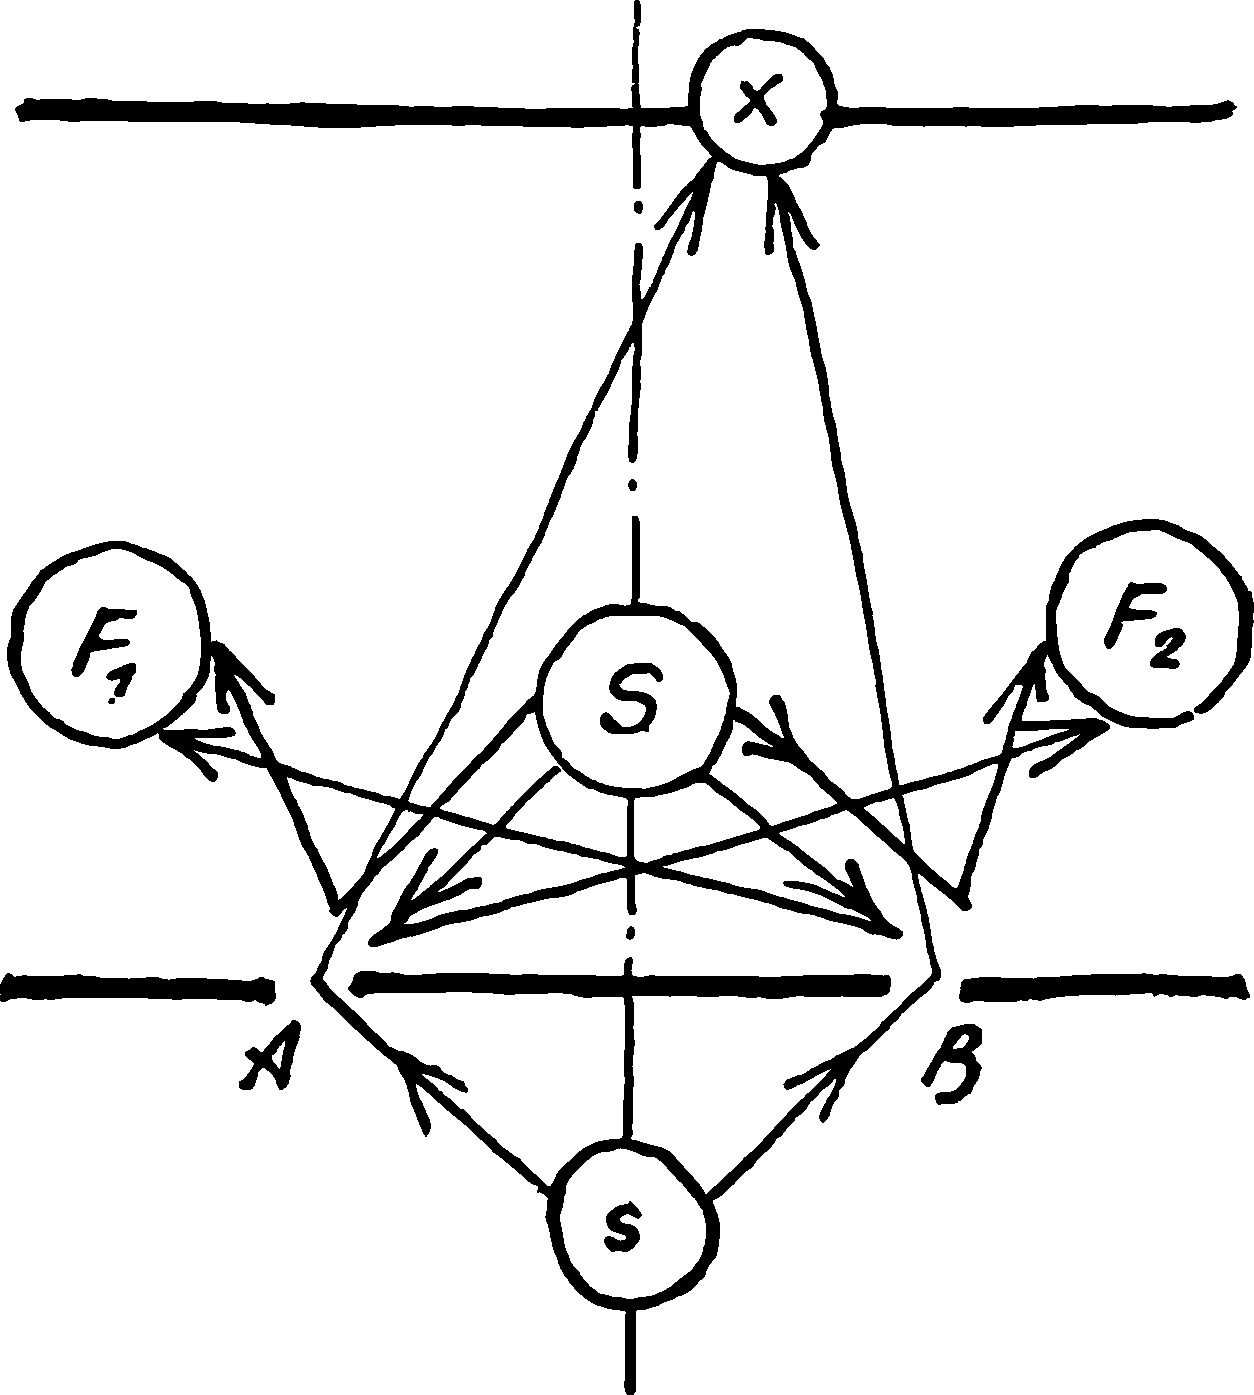
\includegraphics[width=\textwidth]{figures/fig-09-01.pdf}
\caption{Destruction of amplitudes.}
\label{fig-9.1}
\end{marginfigure}

To begin with, we shall assume that the photons scattered in the
vicinity of either of the slits may be registered in the $F_{1}$-state as
well as the $F_{2}$-state (which corresponds to the use of radiation with
a sufficiently large wavelength). In this case, obviously, the photons
don't ``control'' the passage of electrons through the screen with
slits. We denote the transition amplitudes thus: \\[5pt]
for electrons
\begin{equation}%
\begin{split}
\Braket{x|A}\Braket{A|s} & = \varphi_{1} \\
\Braket{x|B}\Braket{B|s} & = \varphi_{2} 
\end{split}
\label{eq-9.5}
\end{equation}

for photons (taking into account the symmetry of the photon transition which can be clearly seen from \hyperref[fig-9.1]{Figure \ref{fig-9.1}})
\begin{equation}%
\begin{split}
\Braket{F_{1}|A}\Braket{A|S}  = \Braket{F_{2}|B}\Braket{B|S} & = \psi_{1} \\
\Braket{F_{2}|A}\Braket{A|S}  = \Braket{F_{1}|B}\Braket{B|S} & = \psi_{2} 
\end{split}
\label{eq-9.6}
\end{equation}

Using these notations and result (\ref{eq-8.11}), we write the following expression for the probability amplitude of simultaneously registering an electron at point $x$ and a photon in the $F_{1}$-state
\begin{equation}%
\Braket{xF_{1}| sS} = \varphi_{1} \psi_{1} + \varphi_{2} \psi_{2}
\label{eq-9.7}
\end{equation}

Correspondingly, for the probability amplitude of simultaneously registering the electron at point $x$ and the photon in the $F_{2}$-state, we write
\begin{equation}%
\Braket{xF_{2}| sS} = \varphi_{1} \psi_{2} + \varphi_{2} \psi_{1}
\label{eq-9.8}
\end{equation}

The probability of an electron being registered at point $x$, independent of where the photon is registered, is of the form (according to second rule from \hyperref[sec-08]{Section \ref{sec-08}})

\begin{equation}%
|\Braket{x| s}|^{2} = |\Braket{xF_{1}| sS}|^{2} + |\Braket{xF_{2}| sS}|^{2}
\label{eq-9.9}
\end{equation}

Substituting (\ref{eq-9.7}) and (\ref{eq-9.8}) into this, we find
\begin{equation}%
\begin{split}
|\Braket{x| s}|^{2} & =  (|\varphi_{1}|^{2}+|\varphi_{2}|^{2}) +
(|\psi_{1}|^{2}+|\psi_{2}|^{2})\\
& + (\varphi_{1}\varphi_{2}^{*}+\varphi_{1}^{*}\varphi_{2})(\psi_{1}\psi_{2}^{*}
+ \psi_{1}^{*}\psi_{2})
\end{split}
\label{eq-9.10}
\end{equation}

Thus the resulting probability of the electronic transition $s \to x$
is made up of two components. The first is the sum of the
probabilities of transitions through slits $A$ and $B$ (considered
separately) multiplied by $(|\psi_{1}|^{2}+|\psi_{2}|^{2})$. The
second component has an interference character; it is due to the
interference of amplitudes. Because of the existence of this
component, we observe the interference distribution of the
impingements of electrons on the detector screen.


Thus, when the photons don't ``control'' the passage of electrons
through a screen with slits, we observe the interference effect
described by the expression (\ref{eq-9.10}). 

Remember that in the example considered here we assumed a sufficiently
long wavelength for the radiation. Let us now reduce the
wavelength. This will lead to a reduction in the probability of a
photon scattered by an electron falling in the ``alien'' counter (for
example, the probability of a photon scattered near slit $A$ being
detected by counter $F_{2}$). This means that with a decrease in the
radiation wavelength, the amplitude $\psi_{2}$ must decrease. A
decrease in the amplitude $\psi_{2}$ will also decrease the relative
contribution of the interference component as is seen clearly from
(\ref{eq-9.10}). As a result, the interference pattern observed on the detector
screen gets blurred. For a sufficiently small radiation wavelength, it
is possible to accurately ``control'' the passage of electrons through
a screen with slits. In this extreme case a photon scattered near
either of the slits arrives only at its ``own'' detector. This means
that $\psi_{2} = 0$. Substituting this result in (\ref{eq-9.10}) we get

\begin{equation}%
|\Braket{x|s}|^{2} = |\psi_{1}|^{2}  (|\varphi_{1}|^{2}+|\varphi_{2}|^{2}) 
\label{eq-9.11}
\end{equation}

Thus, ``control'' of the passage of electrons through a screen with slits leads to a destruction of the interference amplitudes, and consequently to a disappearance of the interference distribution of the electrons Impingements on the detector screen. The result (\ref{eq-9.11}) is in complete accord with (\ref{eq-8.14}). ``Control'' makes the alternatives corresponding to the passage of an electron through different slits distinguishable.


From this example we see that there is a subtle point involved in the
question of the distinguishability of alternatives: in addition to the
complete indistinguishability and complete distinguishability, there
is a continuous spectrum of intermediate situations which should be
identified with partial distinguishability. The result (\ref{eq-9.11})
describes the limiting case of complete indistin- guishability of the
alternatives under consideration ($\psi_{2} =0$). The opposite extreme case
of the complete indistinguishability of alternatives envisages equal
probabilities for a photon falling on its ``own'' or the ``other''
detector: $\psi_{1} = \psi_{2}$. In this case it is easy to see that expression
(\ref{eq-9.10}) assumes the form

\begin{equation}%
|\Braket{x|s}|^{2} = 2 |\psi_{1}|^{2} |\varphi_{1}^{2} + \varphi_{2}^{2}|^{2}
\label{eq-9.12}
\end{equation}

Results (\ref{eq-9.11}) (the squares of the moduli of electron amplitudes are added) and (\ref{eq-9.12}) (the electron amplitudes themselves are added up) are obtained from (\ref{eq-9.10}) as particular (limiting) cases. The general expression (\ref{eq-9.10}) describes the intermediate situation corresponding to partial distinguishability of the alternatives under consideration, differing from one another by the magnitude of the interference component. The less the interference component is the greater is the degree of distinguishability of alternatives.

Thus, distinguishability and indistinguishability are by no means
discrete. Complete indistinguishability is continuously transformed
into complete distinguishability through \emph{intermediate}
situations corresponding to \emph{partial distinguishability}. In
\hyperref[sec-10]{Section \ref{sec-10}} we shall return to the
question of partial distinguishability from the point of view of the
principle of superposition.\sidenote{ Partial distinguishability of alternatives is described in detail in \cite{helfer-1975}.}


We \marginnote{Scattering of Microparticles end Interference of
  Amplitudes} turn to experiment 4 of \hyperref[sec-07]{Section
  \ref{sec-07}}. Let $s_{1}$ and $s_{2}$ be the initial states of the
colliding microparticles and $f_{1}$ and $f_{2}$ be the final states
registered by the corresponding counters. In \hyperref[sec-07]{Section
  \ref{sec-07}} we considered the scattering through an angle of
\ang{90} in the centre of mass system of the colliding particles. For
a more general approach, we shall consider scattering through an angle
$\theta$. In this case the counters are arranged along a straight line
at an angle $\theta$ with the initial direction of the colliding
particles -- see \hyperref[fig-9.2]{Figure \ref{fig-9.2}(a)} (the analysis is carried out, as before, in the centre of mass system of particles).

If upon scattering one microparticle undergoes a transition $s_{1} \to
f_{1}$ and the other a transition $s_{2} \to f_{2}$
(\hyperref[fig-9.2]{Figure \ref{fig-9.2}(b)}), the scattering
amplitude has the form 

\begin{equation}%
\varphi (\theta) = \Braket{f_{1} | s_{1}} \Braket{f_{2} | s_{2}}
\label{eq-9.13}
\end{equation}

Another alternative is also possible: one microparticle undergoes a transition $s_{1} \to f_{2}$ and the other, $s_{2} \to f_{1}$ (\hyperref[fig-9.2]{Figure \ref{fig-9.2}(c)})). In this case the scattering amplitude has the form

\begin{equation}%
\varphi (\pi - \theta) = \Braket{f_{2} | s_{1}} \Braket{f_{1} | s_{2}}
\label{eq-9.14}
\end{equation}

Suppose that the microparticles are \emph{completely distinguishable}. This may mean, for example, that different kinds of microparticles, or the same kind of microparticles with different spin states are colliding. We first consider a situation when counter $f_{1}$ registers microparticles from $s_{1}$ only and counter $f_{2}$ from $s_{2}$ only. In this case the probability of a simultaneous activation of both counters is
\begin{equation}%
|\varphi (\theta)|^{2} = | \Braket{f_{1} | s_{1}} \Braket{f_{2} | s_{2}}|^{2}
\label{eq-9.15}
\end{equation}

\begin{marginfigure}[1cm]
\centering
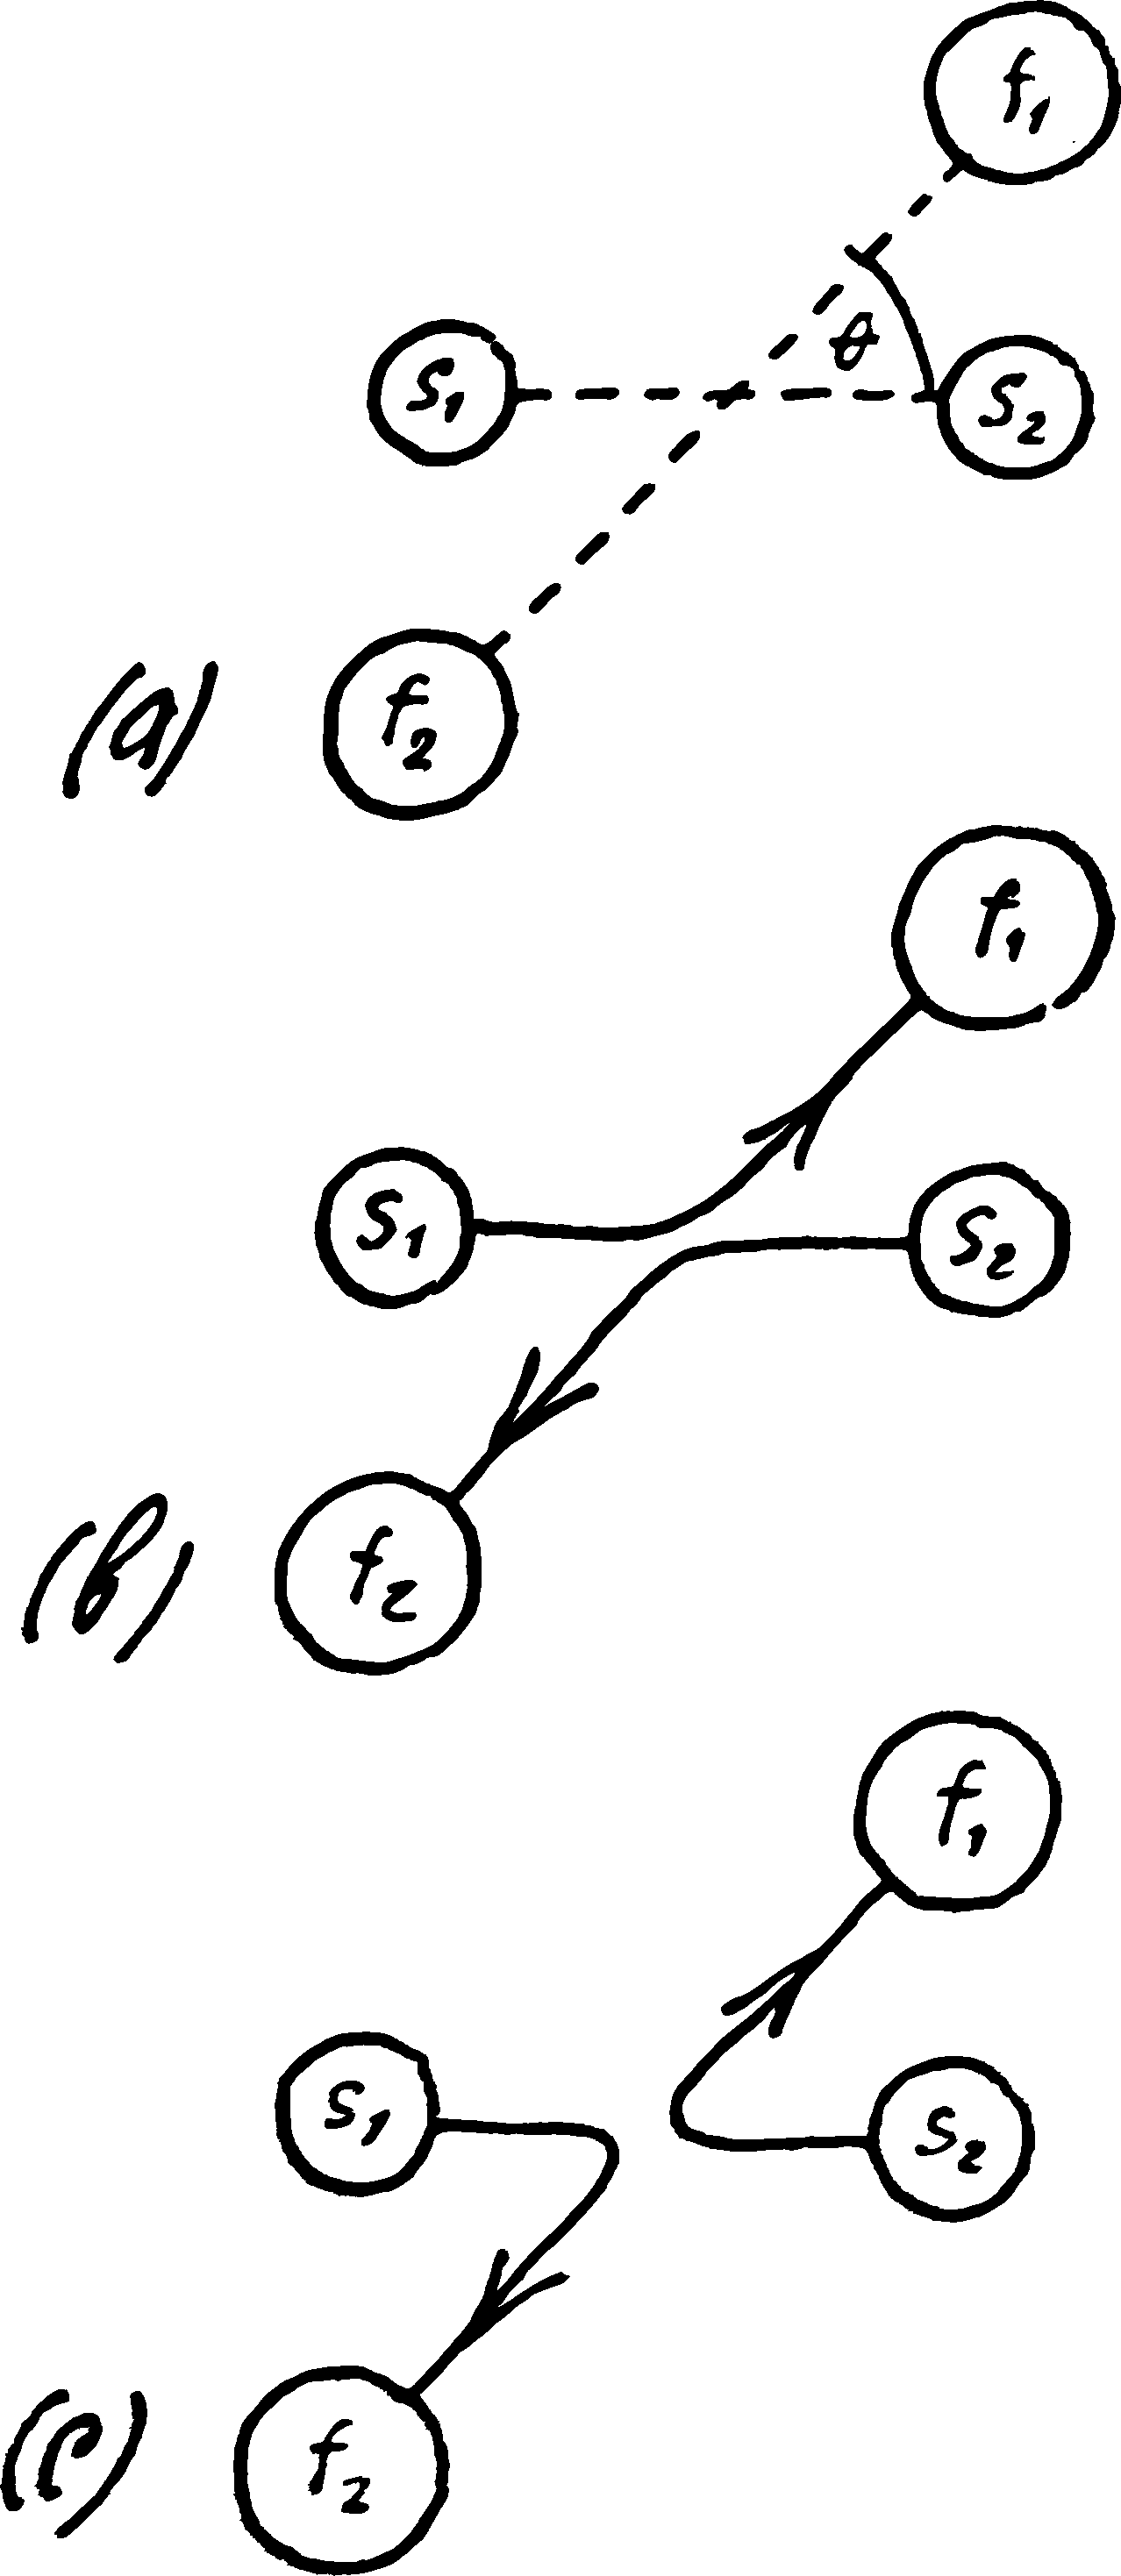
\includegraphics[width=\textwidth]{figures/fig-09-02.pdf}
\caption{Colliding microparticles.}
\label{fig-9.2}
\end{marginfigure}

Second situation: each counter registers any of the microparticles participating in the collision (the situation corresponds to the second example in experiment 4 of \hyperref[sec-07]{Section \ref{sec-07}}). We should now consider two possible alternatives. Since these alternatives are also completely distinguishable for completely distinguishable microparticles, the probability of simultaneous activation of both counters will be given in this case by the expression

\begin{equation}%
|\varphi (\theta)|^{2}+ |\varphi (\pi - \theta)|^{2} = | \Braket{f_{1}
  | s_{1}} \Braket{f_{2} | s_{2}}|^{2} + |\Braket{f_{2}|s_{1}}\Braket{f_{1}|s_{2}}|^{2}
\label{eq-9.16}
\end{equation}

For $\theta = \nicefrac{\pi}{2}$, we get the probability $2| \varphi \, (\nicefrac{\pi}{2}) |^{2}$ -- it is this doubling of probability which we
mentioned in the second example in experiment 4 of \hyperref[sec-07]{Section \ref{sec-07}}.


Further, we assume that the microparticles are \emph{completely indistinguishable}. This means that microparticles of the same type and in the same identical state are considered. Note that the identity of microparticjes mentioned in \hyperref[sec-06]{Section \ref{sec-06}} is a necessary condition for complete indistinguishability.

If the microparticles are completely indistinguishable, so are the
alternatives shown in \hyperref[fig-9.2]{Figure \ref{fig-9.2} (b),
  (c)}. In  this case we should sum not the probabilities of the alternatives, but their amplitudes. The probability of simultaneous activation of the counters should be determined by the expression

\begin{equation}%
w = |\varphi (\theta)|+ \varphi (\pi - \theta)|^{2}
\label{eq-9.17}
\end{equation}
When applied to the third example in experiment 4 of  \hyperref[sec-07]{Section \ref{sec-07}} (when we considered the scattering of $\alpha$-particles by $\alpha$-particles), the result assumes the form

\begin{equation}%
\begin{split}
w &= |\varphi (\nicefrac{\pi}{2})|+ \varphi (\nicefrac{\pi}{2})|^{2}\\
& = 4 |\varphi(\nicefrac{\pi}{2})|^{2}
\end{split}
\label{eq-9.18}
\end{equation}
It is this four-fold increase in the probability $|\varphi
\nicefrac{\pi}{2}|^{2}$ which was observed in the experiment.

Interference of scattering amplitudes is just one of the consequences
of the complete indistinguishability of microparticles. Another
consequence is that the probability of the simultaneous activation of
counters should not change if we interchange $s_{1}$ and $s_{2}$, or,
in other words, if we interchange the scattering amplitudes
$\varphi(\theta)$ and $\varphi(\pi - \theta)$. If we proceed from these consequences, the probability may be formally written in the form

\begin{equation}%
w = |\varphi (\theta)| \pm \varphi (\pi - \theta)|^{2}
\label{eq-9.19}
\end{equation}

The alternative with the ``+'' sign (interfering amplitudes have the
same sign) is already familiar to us -- it is the expression (\ref{eq-9.17}). The other alternative, when the amplitude with opposite signs interfere, is also formally possible. It is remarkable that nature ``employs'' this alternative as well; this can be verified by studying the results of experiments on scattering of electrons by electrons, Thus, we assume that amplitudes with opposite signs interfere:

\begin{equation}%
w_{e} = |\varphi (\theta)| - \varphi (\pi - \theta)|^{2}
\label{eq-9.20}
\end{equation}


and turn to the results of the indicated experiments. For $\theta =
\nicefrac{\pi}{2}$, the probability (\ref{eq-9.20}) vanishes. This
corresponds to the sixth example in experiment 4 of
\hyperref[sec-07]{Section \ref{sec-07}}. We recall that this example
concerned the collision of electrons in the same spin state. It is in
this case that we have two completely indistinguishable alternatives
for the electrons.\sidenote{We shall henceforth omit the word
  ``completely'', but shall always mean it while speaking of
  distinguishable and indistinguishable alternatives. Partial
  distinguishability will be specially mentioned.}


If the colliding electrons are in different spin states (the fifth
example in experiment 4), the alternatives are distinguishable. In
this case the probability of the activation of the counters is given
(as for distinguishable particles) by expression (\ref{eq-9.17}),
which for $\theta = \nicefrac{\pi}{2}$ leads to the familiar result $2
| \varphi (\nicefrac{\pi}{2}) |^{2}$ In the case of non-polarized
electron beams (the fourth example in experiment 4), it should be
remembered that the probability of collision between two electrons in
similar spin states is $\dfrac{1}{2}$. From this, taking
(\ref{eq-9.20}) and (\ref{eq-9.16}) into account, we get the following
expression for the probability of activation of the counters

\begin{equation}%
\begin{split}
w_{e} &= \frac{1}{2} |\varphi (\theta) - \varphi (\pi - \theta) |^{2}\\
& + \frac{1}{2} \left[ |\varphi(\theta)|^{2}+ |\varphi (\pi - \theta)|^{2} \right]
\end{split}
\label{eq-9.21}
\end{equation}

Result (\ref{eq-9.21}) includes the summing of amplitudes (for cases
characterized by indistinguishable alternatives) as well as the
summing of probabilities (for cases characterized by distinguishable
alternatives). For $\theta = \nicefrac{\pi}{2}$, (\ref{eq-9.21}) gives
the probability $w_{e} = |\varphi (\nicefrac{\pi}{2})|^{2}$.This is half the ``classical probability'' (i.e. the probability taking place in the case of indistinguishable alternatives) in complete agreement with the results of the experiments considered in \hyperref[sec-07]{Section \ref{sec-07}}.


Thus, \marginnote{Interference of Amplitudes and Division of
  Microparticles into Bosons and Fermions}we have found that the
experiments on the scattering of microparticles described in
\hyperref[sec-07]{Section \ref{sec-07}} provide a good experimental
background for the concept of the interference of
amplitudes. Moreover, these experiments indicate the necessity for
using not one but two different laws of interference, (\ref{eq-9.17}) and
(\ref{eq-9.20}). We shall discuss the meaning of these two laws, assuming that
$\theta = \nicefrac{\pi}{2}$. According to (\ref{eq-9.17}), we have for $\alpha$-particles
\begin{equation}%
w = 4 | \varphi  \nicefrac{\pi}{2} |^{2}	
\label{eq-9.22}
\end{equation}
and from (\ref{eq-9.20}) we have for the electrons in the same spin state
\begin{equation}%
w_{e} = 0
\label{eq-9.23}
\end{equation}

The use of angle $\theta = \nicefrac{\pi}{2}$ makes the scattering
diagram symmetrical. If in addition we also take into account that the
electrons are in similar spin states ($\alpha$-particles do not have
spin), we may conclude that expressions (\ref{eq-9.22}) and
(\ref{eq-9.23}) describe the probabilities of $\alpha$-particle pairs
and electron pairs, respectively, appearing in the same
state. Comparing this expression with the ``classical probability'' $2
| \varphi (\nicefrac{\pi}{2})|^{2}$, we can come to the conclusion
that one kind of microparticles ($\alpha$-particles in this case)
exhibits a tendency to ``populate'' a given state densely, while other microparticles (electrons in this case), on the contrary, may ``populate'' states only one at a time.

The fact that all microparticles in nature are divided, according to
their behaviour in assemblies of similar particles, into two groups --
\emph{bosons} (with a tendency to densely ``populate'' the same state) and \emph{fermions} (``populating'' the states only one at a time) has already been mentioned in \hyperref[sec-01]{Section \ref{sec-01}}. Now we see that this fundamental fact is associated with the existence of two different laws
for the interference of amplitudes. In the case of bosons, the
amplitudes with like signs interfere; in the case of fermions, it is
the amplitudes with opposite signs that interfere.


Let us consider \marginnote{Bosonic Nature of Photons and Processes of
  Spontaneous and Induced Emission of Light} an example: there are
three atoms emitting photons $(s_{1}, s_{2}, s_{3})$ and three photon
counters $(f_{1}, f_{2}, f_{3})$. The amplitude of probability that
three transitions $s_{1} \to f_{1},\, s_{2} \to f_{2}, \, s_{3} \to f_{3}$
take place simultaneously is $\Braket{f_{1}|s_{1}}
\Braket{f_{2}|s_{2}}\Braket{f_{3}|s_{3}}$. We assume that the photons
are registered in the same state. We then have 3! = 6
indistinguishable alternatives. Besides the one indicated above, the
remaining five amplitudes are given by 
\begin{equation*}%
\begin{split}
&\Braket{f_{1}|s_{2}} \Braket{f_{2}|s_{1}}\Braket{f_{3}|s_{3}},\\
&\Braket{f_{1}|s_{1}} \Braket{f_{3}|s_{2}}\Braket{f_{2}|s_{3}},\\
&\Braket{f_{3}|s_{1}} \Braket{f_{2}|s_{2}}\Braket{f_{1}|s_{3}},\\
&\Braket{f_{1}|s_{2}} \Braket{f_{2}|s_{3}}\Braket{f_{3}|s_{1}},\\
&\Braket{f_{1}|s_{3}} \Braket{f_{2}|s_{1}}\Braket{f_{3}|s_{2}}
\end{split}
\end{equation*}

Assuming that the amplitude of each transition $s_{i} \to f_{k}$ is
the same (we denote it by $a$), and taking into account the
indistinguishability of alternatives, we get, for the amplitude of a
transition with the emission of three photons, the expression $3!
a^{3}$, and for the probability of the transition $(3!)^{2}|a^{3}
|^{2}$. If the alternatives were distinguishable (if distinguishable
microparticles were emitted), the probability would be expressed by
$3! | a^{3}|^{2}$. Generalizing these results for the case of $n$
microparticles, we get for emission probabilities the expressions
$(n!)^{2} | a^{n}|^{2}$ and $n! | a^{n}|^{2}$, respectively.


Let $w_{n}$ be the probability of the emission of n bosons (photons in this case) in the same state, and $W_{n}$ the probability of t.he emission of $n$ distinguishable microparticles in the same state. It is easy to see that
\begin{equation}%
w_{n} = n! W_{n}	
\label{eq-9.24}
\end{equation}

Consequently, the probability of the combined detection of $n$ bosons is $n!$ times greater than the probability of the combined detection of $n$ distinguishable microparticles. We rewrite the result (\ref{eq-9.24}), replacing $n$ by $n + 1$:
\begin{equation}%
w_{n+1} = (n+1)! W_{n+1}	
\label{eq-9.25}
\end{equation}
Dividing (\ref{eq-9.25}) by (\ref{eq-9.24}) we get
\begin{equation}%
\frac{w_{n+1}}{w_{n}} = (n+1) \frac{W_{n+1}}{W_{n}} 
\label{eq-9.26}
\end{equation}
This means that the probability of getting one more boson in a state
where there are already $n$ bosons is $(n + 1)$ times greater than the
probability of getting one more distinguishable microparticle in a
state where there are already $n$ such microparticles. We note further
that for distinguishable microparticles the degree of prior ``population'' of the state is not important. When applied to bosons, it is analogous to the situation when a boson appears in a state which was not occupied earlier. Hence result (\ref{eq-9.26}) may also be interpreted in a different way. The probability of getting another boson in a state having $n$ bosons is $n + 1$ times greater than the probability of a boson appearing in a state which was hitherto unoccupied. In accordance with this interpretation we can rewrite result
(\ref{eq-9.26}) in the form

\begin{equation}%
| \Braket{n + 1 | n} |^{2} = (n + 1) | \Braket{1 | 0}^{2}	
\label{eq-9.27}
\end{equation}

Here we consider a particular state, and $\Braket{1 | 0}$ is the
amplitude of the transition:\\
(unoccupied state) $\to$ (state with one boson), \\
$\Braket{n + 1| n}$ is the amplitude of the transition:\\
(state with $n$ bosons) $\to$ (state with $n + 1$ bosons).
 
When applied to amplitudes and not probabilities, result (\ref{eq-9.27})
means

\begin{equation}%
\Braket{n + 1 | n}  = \sqrt{n + 1}  \Braket{1 | 0}
\label{eq-9.28}
\end{equation}

Let us analyse the result (\ref{eq-9.27}) by considering photon
emission (emission of light). It is easy to see that the probability
of emission is split into two components:
\begin{align}%
|\Braket{n + 1 | s} |^{2}_{s} & =   |\Braket{1 | 0}|^{2}
\label{eq-9.29} \\
|\Braket{n + 1 | n} |^{2}_{i} & =   n|\Braket{1 | 0}|^{2}
\label{eq-9.30} 
\end{align}

The component (\ref{eq-9.29}) describes the probability of
\emph{spontaneous} emission of light and the component (\ref{eq-9.30})
that of \emph{induced emission of light}. In the case of spontaneous
emission, the transitions in a substance (to be more precise, in the
radiating atoms) are spontaneous. They are mutually unrelated and are
independent of external rad iation. In contrast to spontaneous
emission, induced emission depends on the existence of photons near
the radiating atom -- the more photons there are, the greater is the
probability of induced emission. It turns out that on account of their
bosonic nature, the photons ``extract'' as it were, new photons from
the substance. To be more precise, they stimulate transitions in a
substance which lead to the emission of new photons. We stress that a
``stimulated'' photon is created in the same state in which the
``stimulating'' photon was. 


Experiment \marginnote{Absorption of Light and Connection Between the
  Amplitudes of Direct and Reverse Transitions } shows that the
probability of the absorption of light by a substance depends upon the
number of photons in the radiation. In this respect the process of
absorption of light is an induced process. By using the analogy with
(\ref{eq-9.30}) we can write the following expression for the
probability of the annihilation of a photon in a state having $n$
photons:\\
 $|\Braket{n-1|n}|^{2} = n |\Braket{0|1}|^{2}$.

We rewrite this result, replacing $n$ by $(n + 1)$:
\begin{equation}%
|\Braket{n|n+1}|^{2} = (n+1) |\Braket{0|1}|^{2}
 \label{eq-9.31}
\end{equation}
Comparing (\ref{eq-9.31}) with (\ref{eq-9.27}), we conclude that the
probabilities of direct and reverse transitions are equal to each
other:\\ 
 $|\Braket{n+1|n}|^{2} =  |\Braket{n|n+1}|^{2}$.
Thus, using a specific example, we have demonstrated the
so-called principle of \emph{microscopic reversibility}:
\begin{equation}%
|\Braket{f|s}|^{2} = |\Braket{s|f}|^{2}
 \label{eq-9.32}
\end{equation}

When applied to transition amplitudes, this principle means

\begin{equation}%
\Braket{f|s} = \Braket{s|f}^{*}
 \label{eq-9.33}
\end{equation}

Result (\ref{eq-9.33}) supplements the set of four rules applicable to transition amplitudes, which we have considered in \hyperref[sec-08]{Sectio \ref{sec-08}}. It may be treated as an additional, fifth rule.

We \marginnote{Supplementary Examples} shall consider two useful
exarnples which demonstrate the amplitude concepts very clearly.
\begin{marginfigure}[1cm]
\centering
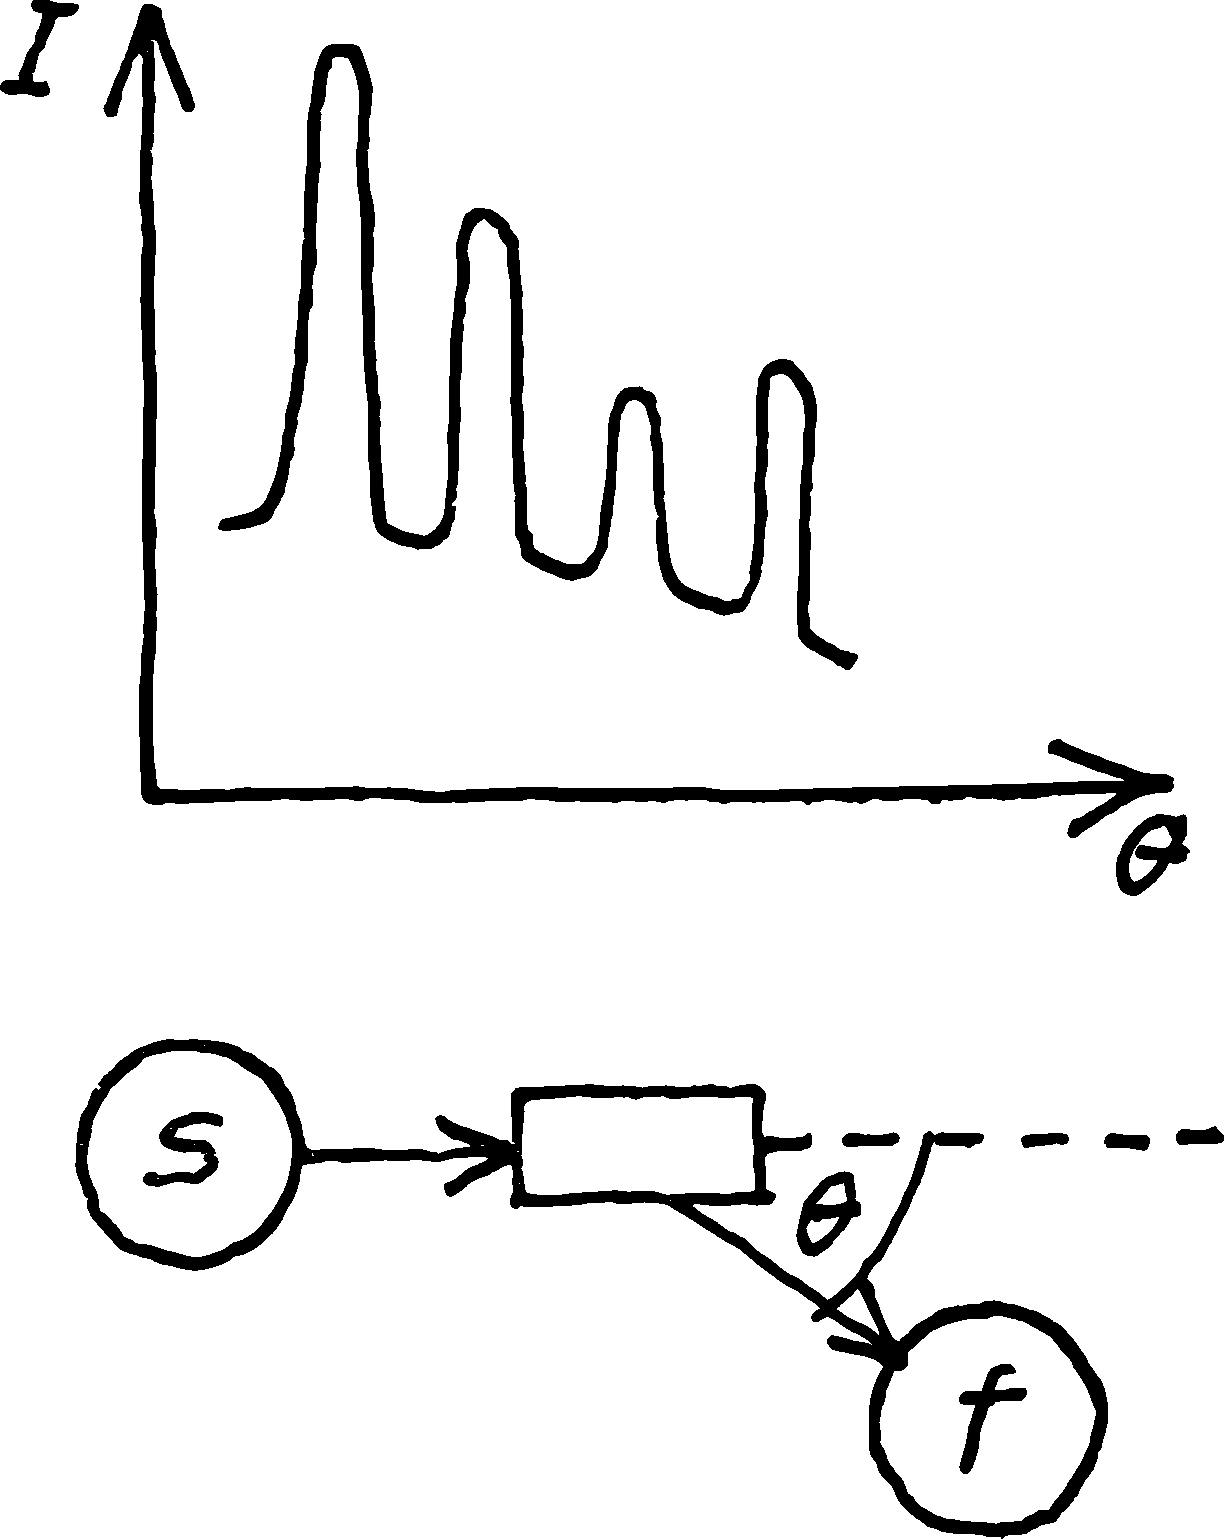
\includegraphics[width=\textwidth]{figures/fig-09-03.pdf}
\caption{Scattering of neutrons by a crystal.}
\label{fig-9.3}
\end{marginfigure}
\emph{Scattering of neutrons by a crystal.} We shall consider the
scattering of very slow neutrons (with energies of the order of
\SI{0.1}{\eV} and lower) by atomic nuclei. It is well known that for
such low energies, the scattering amplitude $\varphi$, considered in the
centre of mass system for a neutron and a nucleus, is independent of
the scattering angle. So, it would appear, the scattering probability
should also be isotropic. However, experiments on the scattering of
very slow neutrons by crystals reveal a strong angular dependence of
the scattering probability. A typical curve is shown in
\hyperref[fig-9.3]{Figure \ref{fig-9.3}}: peaks are observed against a
smooth background. These peaks are a visual demonstration of the
effect of the interference of amplitudes. We shall see how this is so.


Suppose a neutron emerges from its initial $s$-state and is registered
in its final $f$-state. The intermediate $i$-state corresponds to the $i$-th
nucleus in the scattering crystal lattice. According to the third rule
of \hyperref[sec-08]{Section \ref{sec-08}},
\begin{equation}%
\Braket{f|s}_{i} =\Braket{f|i} \varphi \Braket{i|s}
\label{eq-9.34}
 \end{equation}
 We assume that all the $N$ nuclei of the crystal are alike, have zero
 spin, and are located strictly at the lattice points.

 In this case it is impossible in principle to indicate precisely
 which nucleus causes the scattering of the neutron -- the alternatives
 corresponding to the scattering by differently ``numbered'' nuclei
 are indistinguishable. Hence, we must take into account the
 interference of the amplitudes:
\begin{equation}%
\begin{split}
\Braket{f|s} & = \sum_{i}^{N} \Braket{f|s}_{i}  \\
 & = \sum_{i}^{N} \Braket{f|i} \varphi \Braket{i|s}
\end{split}
\label{eq-9.35}
 \end{equation}

Taking (\ref{eq-9.35}) into account, the probability of scattering of the neutron has the form
\begin{equation}%
|\Braket{f|s} |^{2}= |\varphi |^{2} |\sum_{i}^{N} \Braket{f|i}
\Braket{i|s} |^{2}
\label{eq-9.36}
 \end{equation}

On account of the addition of the amplitudes of the scattering at the
nuclei, which are distributed in space in a definite order, a mutual
``cancelling'' of amplitudes is possible in some directions and a
mutual ``enhancement'' in some others; this interference effect is
manifested in the form of sharp peaks for definite scattering angles. 

We further assume that nuclei in the crystal have a spin (let it be
equal to $\nicefrac{1}{2}$, as for neutrons). In this case we should
distinguish between the amplitude of scattering by the nucleus
\emph{with spin inversion} (in accordance with the law of conservation
of momentum, the neutron spin must also he inverted in this case), and
\emph{without spin inversion} of the nucleus (and the neutron),
i.e. between $\chi$ and $\varphi$, respectively. If the scattering of
the colliding microparticles is accompanied by spin inversion, the
corresponding alternative is distinguishable -- it is clear that in such an act of scattering only that nucleus participates whose spin has been inverted. Now the probabilities and not the amplitudes should be summed.


Taking account of the amplitudes $\varphi$ and $\chi$ we can represent the scattering probability of neutrons from $s$-state to $f$-state in the following form:
\begin{equation}%
|\Braket{f|s}|^{2} = |\varphi|^{2} |\sum_{i}^{N} \Braket{f|i}
\Braket{i|s}|^{2} + | \chi |^{2} |\sum_{i}^{N} \Braket{f|i}
\Braket{i|s}|^{2}
\label{eq-9.37}
\end{equation}

The first term on the right-hand side of (\ref{eq-9.37}) accounts for the characteristic interference peaks in \hyperref[fig9.3]{Figure \ref{fig-9.3}}, while the second term is responsible for the smooth background. It is customary to say that the first term describes the probability of the \emph{coherent} scattering, and the second that of the \emph{incoherent} scattering of neutrons.

\emph{Atomic beam in inhomogeneous fields.} Let us assume that a beam
of atoms occupying a certain initial $s$-state (this is a definite
spin state) passes first through one region of non-uniform magnetic
field ($B_{1}$), then through another ($B_{2}$) and is finally
registered in its final spin state $f$. Non-uniform magnetic fields
are used here as factors capable of changing the spin state of the
atoms in the beam. Experiment shows that the probability of the $s \to
f$ transition is different in the cases when 
\begin{enumerate}[label=(\alph*)]
\item  observations are carried out to find the state of the atoms in
  the beam between fields $B_{1}$ and $B_{2}$ , and when 
\item  such observations are not carried out. 
\end{enumerate}

The difference in probabilities $| \Braket{f | s} |^{2}$ in these two cases
is easily explained if we take into account that in case (a) the
intermediate $i$-spin states are fixed each time and, consequently, the
alternatives corresponding to them are distinguishable; hence:
\begin{equation}%
|\Braket{f|s}|^{2} = \sum_{i}|\Braket{f|i}\Braket{i|s}|^{2}
\label{eq-9.38}
\end{equation}
In case (b) the intermediate $i$-states are not fixed and, consequently, the alternatives corresponding to them are indistinguishable. Hence
\begin{equation}%
|\Braket{f|s}|^{2} = | \sum_{i} \Braket{f|i}\Braket{i|s}|^{2}
\label{eq-9.39}
\end{equation}

\begin{marginfigure}[3cm]
\centering
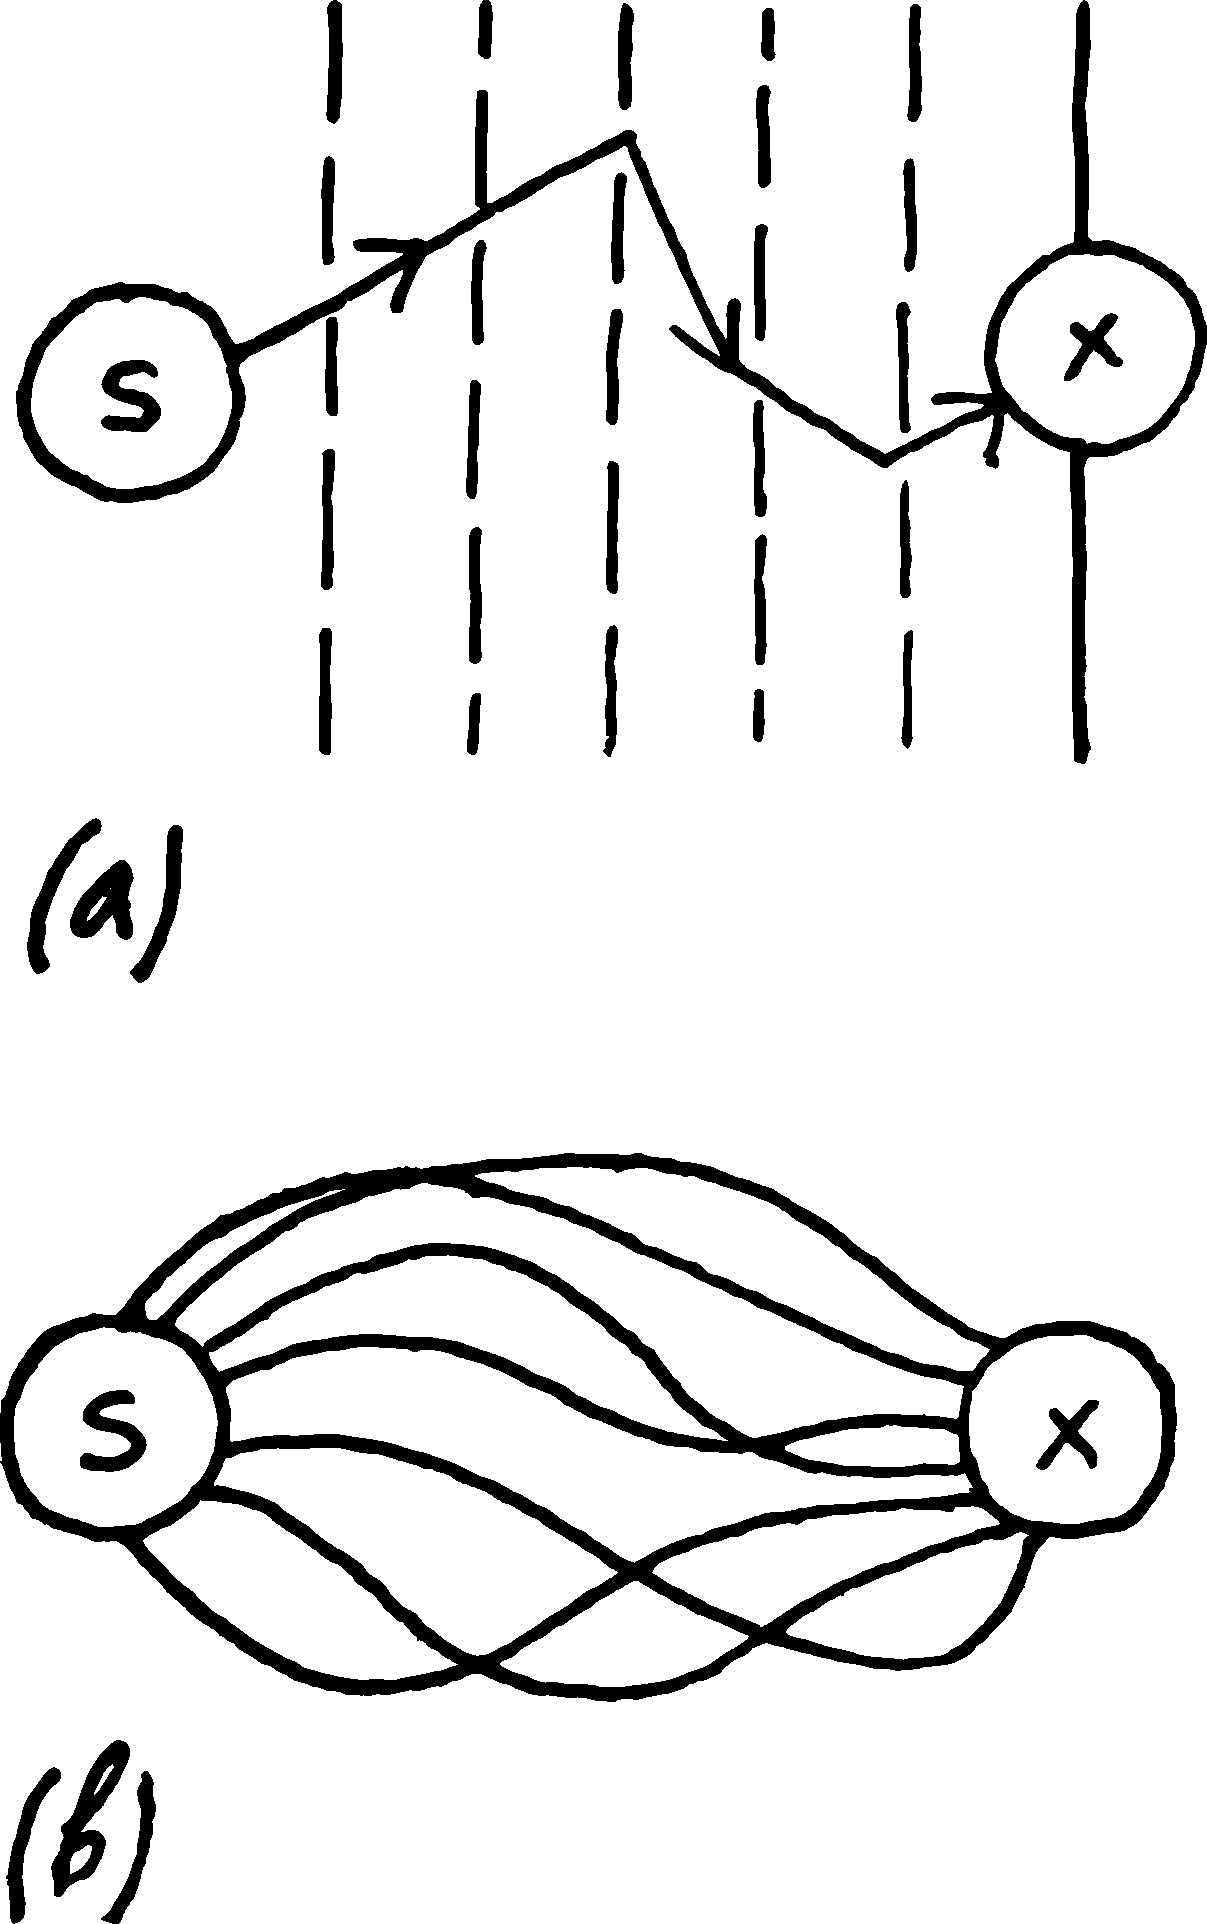
\includegraphics[width=\textwidth]{figures/fig-09-04.pdf}
\caption{Path integral approach.}
\label{fig-9.4}
\end{marginfigure}
\textsc{Feynman's Path Integrals} \textsf{\small In conclusion
  indicate the possibility of a somewhat unusual formulation of
  quantum mechanics, based on amplitude concepts. In the beginning of
  this section, we considered an interferometer in the form of a
  screen with two slits. There were two indistinguishable alternatives
  corresponding to the two interference amplitudes. Let us now assume
  that instead of a screen with two slits, we have a screen with $n$
  slits. The number of alternatives (and, correspondingly, amplitudes)
  will be equal to $n$. Further, we place another screen with $n$
  slits parallel to the first screen; the number of alternatives
  (amplitudes) will rise to $n^{2}$. We shall continue this process by
  placing more and more screens in the space between the source of
  microparticles and the detector screen; moreover, we shall
  simultaneously keep on increasing the number of slits in each
  screen. In the limiting case of an infinitely large number of
  screens and an infinitely large number of slits, we arrive at a
  situation when the entire space between the source and detector
  screen will turn out to be ``filled'' by different `paths' of the
  microparticle, each corresponding to a definite alternative and a
  corresponding definite amplitude (one such path is indicated in
  \hyperref[fig-9.4]{Figure \ref{fig-9.4}(a)}). The total amplitude of
  $s \to x$ transition is the sum (more exactly, the integral) over
  all the possible amplitudes. Finally, we assume that the system of
  screens with slits was introduced only fictitiously; in fact there
  are no screens and the entire space between points $s$ and $x$ is
  ``filled'' by all the possible paths. If we can write the transition
  amplitude for each such trajectory, then the probability of the $s
  \to x$ transition may be found as the square of the modulus of the
  integral summing up all the given amplitudes (called the path
  integrals). In this sense, the quantum-mechanical motion from $s \to
  x$ is nothing but the superposition of a set of classical motions
  (classical trajectories) almost in the same way as indicated in
  \hyperref[fig-9.4]{Figure~\ref{fig-9.4}(b)}. The transition from
  quantum to classical mechanics corresponds to the reduction of the
  given superposition of paths to a certain individual trajectory. }

  \textsf{\small The concept of the motion of a microparticle along classical path
  integrals (in other words, through interference of amplitudes
  corresponding to the classical trajectories) is discussed in detail
  in \hyperref[sec-05]{Section \ref{sec-05}}.}

\section{Superposition of States}
\label{sec-10}
In the previous section, while studying the prohlem of the probability
of the transition of a microparticle from one state to another, we
introduced and discussed the concepts of the transition probability
amplitude, distinguishable and indistinguishable alternatives of
transition, the interference of amplitudes corresponding to
indistinguishable alternatives, all of which are specifically
quantum-mechanical concepts. on the basis of a number of examples the
reader should convince himself of the importance of the concept of
interfering amplitudes, which gives an explanation of the results of
various experiments with microparticles.

The interference of transition amplitudes is inseparably linked with
one of the most fundamental principles of quantum mechanics -- the
\emph{principle of superposition of states}, which reflects the
specific nature of the ``interrelations'' among the states of a
microparticle. We shall now consider this principle.

Earlier, in \hyperref[sec-03]{Section \ref{sec-03}}, we
\marginnote{Principle of Superposition of States} studied the
uncertainty relations. In this connection it was remarked, in
particular, that the states of a microparticle were combined in groups
each of which contained the definite values of anyone complete set of
physical quantities. We also gave examples of complete sets of
values for an electron and a photon. 


Continuing the discussion commenced in \hyperref[sec-03]{Section
  \ref{sec-03}}, we shall introduce notations for the various complete
sets: the $\alpha$-set, the $\beta$-set, the $\gamma$-set, etc. In
this context we shall speak of the group of $\alpha$-states, the group
of $\beta$-states, etc.

We suppose that the microparticle is in one of the $\alpha$-states. It
means that the quantities in the $\alpha$-set have definite
values. But what can we say about the values of the quantities in any
other complete set, for example, the $\beta$-set? According to the
uncertainty relations, the quantities in the $\beta$-set do not have
definite values in the state under consideration. The reader is
justified in taking this as a negative fact. But, fortunately, this is
fully ``compensated'' by a positive circumstance -- the principle of
the superposition of states.


According to the principle of superpostt.ion, there exists a link
between the states of the microparticle, corresponding to different
complete sets: any state from one set may be represented in the form
of a \emph{superposition of states} from another set. Thus, for example, a
given $\alpha$-state may be represented in the form of a superposition of
$\beta$-states. If we arbitranily adopt the symbol $\bra{\;} $ to indicate the state
of a microparticle, the principle of superposition may be written in
the form 
\begin{equation}%
\Bra{\alpha} = \sum_{\beta} \Phi_{\alpha \beta} \Bra{\beta }
\label{eq-10.1}
\end{equation}

The expression (\ref{eq-10.1}) appears as an ``expansion'' of the
given state $\bra{\alpha}$ into the sum of $\beta$-states, the numbers
$ \Phi_{\alpha \beta}$ playing the role of coefficients in the
expansion. More concretely, the number $\Phi_{\alpha \beta}$ is the
amplitude of the probability that we shall obtain values corresponding
to the state $\bra{\beta}$ while measuring the quantities from the
$\beta$-set in the state $\bra{\alpha}$. In other words, it is the
amplitude of the probability that a microparticle in state $\bra{\alpha}$, may
also be found in the state $\bra{\beta}$. If we denote this amplitude by the
usual symbol $\Braket{\alpha|\beta}$, expression (\ref{eq-10.1})
assumes the following form:
\begin{equation}%
\Bra{\alpha} = \sum_{\beta} \Braket{\alpha |\beta} \Bra{\beta }
\label{eq-10.2}
\end{equation}

In the preceding sections we considered the amplitudes of the
transition probability (in short, transition amplitudes). At first
glance, the principle of superposition ``brings into play'' a new type
of amplitudes of probability. Actually, the above-mentioned expression
``$\Braket{\alpha | \beta}$ is the amplitude of the probability that a
microparticle in state $\bra{\alpha}$ may also be found in state
$\bra{\beta}$'' allows another obvious interpretation:
``$\Braket{\alpha | \beta}$ is the amplitude of the probability of a
microparticle arriving in state $\bra{\beta}$, if it is known that the
given particle actually exists in state $\bra{\alpha}$''. In short,
the latter statement means that $\Braket{\alpha | \beta}$ is the
amplitude of the probability with which any $\beta$-state is
``represented'' in a given $\alpha$-state. This produces the
impression that the amplitudes $\Braket{\alpha | \beta}$ don't have
anything to do with any transitions or processes. Considering this
impression, we introduce a new term for $\Braket{\alpha | \beta}$ --
the \emph{amplitude of probability of state} (in brief, the
\emph{amplitude of state}).



The reader must be warned at once that the above impression is
erroneous. However, in order to be convinced of this, we must analyse
the process of measurement. Measurement in quantum mechanics will be
discussed in \hyperref[sec-11]{Section \ref{sec-11}}. This discussion
will necessitate some correction in the above definition of the
amplitudes $\Braket{\alpha | \beta}$ and will enable us to actually
reduce the amplitudes of states to the already familiar amplitudes of
transitions.

But everything has its own time, and so, for the time being, we shall
operate with the concept of ``amplitude of state'' as an independent
concept, without ascertaining the practical meaning of, say, the
phrase ``a particle in state $\bra{\alpha}$ can also be found in state $\bra{\beta}$''.

As has been noted earlier, the principle of superposition
``supplements'', as it were, the uncertainty relations; its positive
content ``compensates'' the well-known negative aspect of these
relations. Figuratively speaking, the uncertainty relations indicate
the ``old'' concept which must be rejected while we go over from
macrophenomena to microphenomena. In particular, they require a
rejection of the simultaneous measurahiltty of all physical quantities
characterizing a given object. At the same time, the principle of
superposition indicates the ``new'' concept which is applicable when
considering microparticles; superposition (\ref{eq-10.2}) means that if a
microparticle is in a state in which the quantities of the $\alpha$-set are
measurable, then the value of the quantities in the $\beta$-set may be predicted with a probability equal to $|\Braket{\alpha|\beta}|^{2}$.

  In \marginnote{Superposition in Classical Physics and Quantum
    Mechanics} classical physics one comes across superposition quite
  frequently, the foremost example being ihe well-known superposition
  of classical waves. From a mathematical point of view, the classical
  superposition and superposition in quantum mechanics are
  analogous. This circumstance greatly stimulated the development of
  quantum theory. At the same time, it certainly complicated the
  interpretation of the physical content of theoretically obtained
  results since it tempted one to draw erroneous analogies with
  classical waves. In the words of Dirac \cite{dirac-1958} \emph{the assumption of
  superposition relationships between the states leads to a
  mathematical theory in which the equations that define a state are
  linear in the unknowns. In consequence of this, people have tried
  to establish analogies with systems in classical mechanics, such as
  vibrating strings or membranes, which are governed by linear
  equations and for which, therefore, a superposition principle
  holds \ldots} (remember the criticism in \hyperref[sec-05]{Section \ref{sec-05}} of the attempts to represent the motion of a bound microparticle with the· help of
  classical waves in a resonator -- author's remarks). \emph{It is important to
  remember, however, that the superposition that occurs in quantum
  mechanics is of an essentially different nature from any occurring
  in the classical theory, as is shown by the fact that the quantum
  superposition principle demands indeterminacy in the results of
  observations.}

Speaking of the difference between quantum and classical
superpositions, remember that a superposition of two classical waves
leads to the generation of a new wave having, of course, new
characteristics. However, a superposition of two states
$\bra{\beta_{1}}$ and  $\bra{\beta_{2}}$, characterized by the values $\beta_{1}$ and $\beta_{2}$ respectively, of quantities in the $\beta$-set, by no means leads to a state having any new value of $\beta$. As an example, let us consider a certain superposition of states 
\begin{equation*}
\Braket{\alpha | \beta_{1}} \bra{\beta_{1}} + \Braket{\alpha | \beta_{2}} \bra{\beta_{2}} 
\end{equation*}

We shall measure the $\beta$-quantity in this state. As a result, we
get every time one of the earlier values, $\beta_{1}$ or
$\beta_{2}$. Moreover, it is impossible to accurately predict which of
the two states will be obtained in any particular measurement. We can
only indicate the probability of getting $\beta_{1}$ or $\beta_{2}$
These probabilities are equal to $|\Braket{\alpha | \beta_{1}}|^{2}$
and $|\Braket{\alpha | \beta_{2}}|^{2}$, respectively. It is this
specific \emph{uncertainty in the results of measurements} that
determines the fundamental difference between quantum and classical
superpositions.

Taking into consideration the quantum-mechanical principle of
superposition, let us return to the question of quantum transitions
discussed in \hyperref[sec-02]{Section \ref{sec-02}}. Suppose we
consider, as before, two energy levels $E_{1}$ and $E_{2}$ of the
microparticle. We denote the corresponding states of the particle in
which it has energy $E_{1}$ or $E_{2}$ (i.e. is on the first or second
level) through $\bra{1}$ and $\bra{2}$ respectively. According to the
principle of superposition, in addition to states $\bra{1}$ and $\bra{2}$ we can
also get the state
\begin{equation}
\bra{f} = \Braket{f|1} \bra{1} + \Braket{f|2} \bra{2}
\label{eq-10.3} 
\end{equation}

Measurement of energy of the microparticle in this state leads either
to the result $E_{1}$ or to the result $E_{2}$ (as if the
microparticle were on the level $E_{1}$ and simultaneously on the
level $E_{2}$). The first result is obtained with the probability
$|\Braket{f|1}|^{2}$, and the second, with the probability
$|\Braket{f|2}|^{2}$ The possibility, of the existence of such a
specific quantum-mechanical situation immediately removes the basic
contradiction of the quantum transition, mentioned in
\hyperref[sec-02]{Section \ref{sec-02}}. It is sufficient to assume
that an interaction of a microparticle with radiation leads to a
superposition state of the type (\ref{eq-10.3}). Then the probability of
finding a particle on one energy level or another (on its earlier
level or on a new one) will be described simply by the square of the
modulus of the corresponding amplitude of state.



In \marginnote{Mutually Orthogonal States: Total and Partial
  Distinguishability of States} order to finally convince ourselves
that the quantum-mechanical principle of superposition has in fact
nothing in common with the classical superposition we turn to
expression (\ref{eq-10.2}) and see how it changes upon the transition to
classical physics. Since in classical physics all the quantities can
be simultaneously measured, they form together one ``complete
set''. Considering that the superposition bonds described by relation
(\ref{eq-10.2}) operate between different complete sets, we arrive at the
conclusion that in the classical case such bonds simply do not exist
and, consequently, all formally composed amplitudes of states must be
taken as being equal to zero:
\begin{equation}
\Braket{\alpha | \beta} = 0 
\label{eq-10.4} 
\end{equation}
In quantum mechanics condition (\ref{eq-10.4}) also exists, but only
``within the limits'' of the given complete set (for states belonging to
the same set). Thus, for example,
\begin{equation}
\Braket{\alpha_{i} | \alpha_{j}} = 0, \,\, \mathrm{if} \,\, i \ne j
\label{eq-10.5} 
\end{equation}

The amplitude of a state is equal to zero if and only if the two
corresponding states are \emph{mutually independent} (if an object is
in one of these states, it cannot be found in the other). Such states
are called \emph{mutually orthogonal}. In this respect all the states
of a classical particle are mutually orthogonal, while in quantum
mechanics only the states belonging to the same complete set are
orthogonal and the states belonging to different sets are
non-orthogonal. This last fact is reflected in the principle of
superposition of states.

The idea of mutually orthogonal states permits us to define more
precisely the concept of complete and partial distinguishability. For
this purpose it is convenient to make use of the above-mentioned
example of the scattering of microparticles of one type by one
another. Since such particles are identical, their distinguishability
is determined by the distinguishability of states (states
$\bra{s_{1}}$ and $\bra{s_{2}}$; see \hyperref[sec-09]{Section
  \ref{sec-09}}). We recall that in \hyperref[sec-09]{Section
  \ref{sec-09}} we discussed, in particular, microparticles of the
same kind but in different spin states, as examples of completely
distinguishable microparticles. We thus tacitly assumed that different
spin states are completely distinguishable. We can now clearly
indicate the criterion of complete and partial distinguishability of
states: if $\Braket{s_{1}| s_{2}} =0$, the states $\bra{s_{1}}$ and
$\bra{s_{2}}$ are completely distinguishable; there are no
superposition bonds between them. But if $\Braket{s_{1}| s_{2}} \ne
0$, the states under consideration are partially distinguishable. In
other words, orthogonality of states is the criterion of their
complete distinguishability.

Suppose we are considering scattering of two bosons of the same
type. The result (\ref{eq-9.16}) will hold good if the initial states
are mutually orthogonal (let these states be $\bra{\alpha_{1}}$ and
$\bra{\alpha_{2}}$. The result (\ref{eq-9.17}) will be valid if the
  initial states are similar (say, $\bra{\alpha_{1}}$ and
  $\bra{\alpha_{1}}$. Both these results are just two extreme cases
  corresponding to complete distinguishability and complete
  indistinguishability of microparticles, respectively. However,
  different intermediate situations corresponding to partial
  distinguishability are possible, when the initial states of
  microparticles are a superposition of several mutually orthogonal
  states:
\begin{equation}
\begin{split}
\bra{s_{1}} & = \Braket{s_{1} | \alpha_{1}}\bra{\alpha_{1}} +
\Braket{s_{1} | \alpha_{2}}\bra{\alpha_{2}}, \\
\bra{s_{2}} & = \Braket{s_{2} | \alpha_{1}}\bra{\alpha_{1}} +
\Braket{s_{2} | \alpha_{2}}\bra{\alpha_{2}}
\end{split}
\label{eq-10.6}
\end{equation}
It can be shown (see \emph{Gibbs' Paradox and Identity in Quantum Mechanics}
\cite{helfer-1975}) that in this case the probability of simultaneous
activation of detectors is determined by the expression

\begin{equation}
\begin{split}
w = |\varphi(\theta)|^{2} + |\varphi(\pi - \theta)|^{2} +
|\Braket{s_{1}|s_{2}}|^{2} \left[ \varphi(\theta) \varphi^{*}(\pi -
  \theta) 
 + \varphi^{*}(\theta) \varphi(\pi - \theta) \right]
\end{split}
\label{eq-10.7}
\end{equation}

For $| \Braket{s_{1}|s_{2}}|^{2} \to 0$, the result (\ref{eq-10.7})
  turns into (\ref{eq-9.16}) (we come to the limiting case of complete
  distinguishability).

  Thus, we find that the question of the complete and partial
  distinguishability of alternatives in quantum mechanics is closely
  linked with the quantum-mechanical principle of superposition,
  more precisely, with the mutual orthogonality or non-orthogonality
  of states.

  The \marginnote{Basic States} different states corresponding to the
  same complete set of quantities are called \emph{basic} states
  (eigenstates). The amplitudes of elementary states satisfy the
  condition
  \begin{equation}
\Braket{a_{i}|a_{j}} = \delta_{ij},
\label{eq-10.8}
\end{equation}  
where $\delta_{ij}$ is the so-called Kronecker delta symbol; it is
equal to zero for $i \ne j$ and unity for $i = j$. The expression
(\ref{eq-10.8}) is called the \emph{condition of orthonormalization of
  basic states}. It is obtained by taking into consideration
(\ref{eq-10.5}) and the fact that the probability of getting the value
$\alpha_{i}$ in the state $\bra{\alpha_{i}}$ is obviously equal to
unity. The important property of the system of basic states is its
\emph{completeness}: any state may be expanded in a system of
elementary states.

Basic states may be selected in different ways depending on the
complete set under consideration. Thus, different systems of basic
states may be used: $ \left\{ \bra{\alpha_{i}} \right\}, \; \left\{ \bra{\beta_{i}} \right\} $ etc. It is said that \emph{different
  representations} are possible. For a more general approach, the
principle of superposition of states signifies the fact that any
state $\bra{f}$ of a microparticle may he expanded in any system of basic
states: 
\begin{equation}
\begin{split}
\bra{f} & = \sum_{i} \Braket{f|\alpha_{i}} \bra{\alpha_{i}} \\
\bra{f} & = \sum_{i} \Braket{f|\beta_{i}} \bra{\beta_{i}} 
\end{split}
\label{eq-10.9}
\end{equation}

The \marginnote{ Superposition of States and Passage of Photons
  Through Polarizers} principle of superposition permits an
explanation of the results of experiment 3 in
\hyperref[sec-07]{Section \ref{sec-07}}. Using this principle, we
shall consider the passage of individual photons through the system of
three polarizers shown in \hyperref[fig-7.6]{Figure \ref{fig-7.6}}. We
denote the state of polarization of a photon after the first
polarization by $\bra{s}$. According to the principle of superposition, the
state $\bra{s}$ may be considered as a superposition of the basic states
$\bra{1}$ and$\bra{2}$, corresponding to two independent polarizations of the
photon-along and perpendicular to the axis of the second polarizer,
respectively:
\begin{equation}
\bra{s} = \Braket{s|1} \bra{1} + \Braket{s|2} \bra{2}
\label{eq-10.10}
\end{equation}
(note that in this example, the system of basic states contains only
two states). The amplitudes of the states may be written in this case
in the form $\Braket{s|1} = \cos \alpha$ and $\Braket{s|2} = \sin
\alpha$. Thus,
\begin{equation}
\bra{s} = \cos \alpha \bra{1} + \sin \alpha \bra{2}
\label{eq-10.11}
\end{equation}

The second polarizer lets through photons from the state $\bra{1}$
only. Since according to (\ref{eq-10.11}) the state $\bra{1}$ is
``represented'' in state $\bra{s}$ with a probability $\cos^{2}
\alpha$, out of $N$ photons only $N \cos^{2} \alpha$: photons will
pass through the second polarizer. Moreover, all the photons that pass
will appear in the state $\bra{1}$ (i.e. they will be polarized long the
axis of the second polarizer). Thus, in front of the second polarizer,
the photon exists as if partially in the state $\bra{1}$ and partially in
the state $\bra{2}$. At the instant when the photon passes through the
polarizer, this ``duality'' vanishes. In some cases a photon exists in
the state $\bra{2}$ and so cannot pass through the polarizer, while in some
other cases it is in the state $\bra{1}$ and can thus pass through the
polarizer. Further, for any individual photon it is impossible to
predict in which state it will appear (hence it is impossible to
predict whether a given photon will pass through the polarizer or
not).

While studying the passage of photons through the third polarizer, we
proceed in a similar way. The state $\bra{1}$ Iis expanded into a system of
basic states $\bra{1'}$ and $\bra{2'}$ corresponding to a polarization of photon
along or perpendicular to the axis of the third polarizer: 
\begin{equation}
\bra{1} = \sin \alpha \bra{1'} + \cos \alpha \bra{2'}
\label{eq-10.12} 
\end{equation}
The third polarizer lets through photons in the state $\bra{1'}$
only. This state is ``represented'' in the state $\bra{1'}$ with a
probability $\sin^{2} \alpha$. Hence out of $N \cos^{2} \alpha$,
photons only $N \cos^{2} \alpha sin^{2} \alpha$ photons will pass
through the third polarizer, all these photons being in the state
$\bra{1'}$. If we now remove the second polarizer, then in place of
(\ref{eq-10.11}) and (\ref{eq-10.12}) we get
\begin{equation}%
  \bra{s} = \Braket{s|1'} \bra{1'} + \Braket{s|2'} \bra{2'}
\label{eq-10.13} 
\end{equation}
where, as can be easily seen, $\Braket{s|1'} = 0$ and $\Braket{s|2'}
=1 $, so that $\bra{s} = \bra{2'}$. Naturally, in this case, at the
outlet of the system of polarizers no photons are observed at all.

Let the transition \marginnote{Principle of Superposition of States
  and Interference of Transition Amplitudes}from state $\bra{s}$ to
state $\bra{f}$ take place through certain intermediate $v$-states. We
suppose that the microparticle is not fixed in the intermediate state
so that a case of physically indistinguishable alternative takes
place. In this case, as we know, the transition amplitude
$\Braket{f|s}$ given by the expression
\begin{equation}%
\Braket{f|s} = \sum_{i} \Braket{f|v_{i}}\Braket{v_{i}|s} 
\label{eq-10.14} 
\end{equation}
where $\Braket{f|v_{i}}$ and $\Braket{v_{i}|s}$ are the amplitudes of the respective
transitions. The intermediate $v$-states must be completely
distinguishable, since otherwise there is no point in introducing the
concept of distinguishable or indistinguishable alternatives, since
the very concept of alternatives loses its meaning. Consequently, the
$v$-states must form a system of mutually orthogonal basic
states. Taking this into consideration, we make use of the principle
of superposition and express the state $\bra{f}$ in the form
\begin{equation}%
\bra{f} = \sum_{i} \overline{\Braket{f|v_{i}}}\bra{v_{i}}
\label{eq-10.15}
\end{equation}
      
where the amplitudes $\overline{\Braket{f|v_{i}}}$ are essentially the
amplitudes of the states (the bar is used to distinguish the amplitude
of the state from the transition amplitude $\Braket{f|v_{i}}$). If
superposition (\ref{eq-10.15}) exists, there is actually no need to
perform a transition from $\bra{s}$ to $\bra{f}$. Since the state
$\bra{f}$ is a superposition of states $\bra{v_{i}}$, it is sufficient
to simply accomplish transitions from the state $\bra{s}$ to each of
the states $\bra{v_{i}}$· This means that the transition amplitude $\Braket{f|s}$ is a superposition of the transition amplitudes $\Braket{v_{i}|s}$:
\begin{equation}%
\Braket{f|s} = \sum_{i} \overline{\Braket{f|v_{i}}}\Braket{v_{i}|s}
\label{eq-10.16} 
\end{equation}

Comparing (\ref{eq-10.16}) and (\ref{eq-10.14}) we conclude that 
\begin{equation}%
\overline{\Braket{f|v_{i}}} = \Braket{f|v_{i}}
\label{eq-10.17} 
\end{equation}
This means that at the level of mathematical apparatus, we have
accomplished a reduction of the amplitudes of the states to transition
of amplitudes. In other words, the amplitudes of the states in fact
play the same role in the apparatus of quantum mechanics as the
transition amplitudes. Incidentally, we have also established that
relations (\ref{eq-10.14}) and (\ref{eq-10.15}) are closely related to each other and
hence the effect of the interference of transition amplitudes and
the principle of the superposition of states are directly
interrelated.

In conclusion, we mention an important method which is widely applied
in quantum mechanics. It is easy to see that if we delete the sign of
the initial and final states in the expression for the interference of
amplitudes, we automatically obtain the superposition expression for
the undeleted state. Thus, if in (\ref{eq-10.14}) we delete $\bra{s}$ on the left-
and right-hand sides of the equation, we obtain the superposition
expression (\ref{eq-10.11}) for the state $\bra{f}$ (note that in addition to the
symbol $\bra{}$, the symbol $\ket{}$ is used for denoting a state).

We shall demonstrate \marginnote{The Mechanics of Quantum Mechanics}
the basic methods reflecting, in Feynman's words, the ``mechanics of
quantum mechanics''. Let us delete the state $\bra{f}$ from the left- and
right- hand sides of equation (\ref{eq-10.14}). This gives
\begin{equation}%
\bra{s} = \sum_{i} \bra{v_{i}} = \Braket{v_{i}|s}
\label{eq-10.18} 
\end{equation}

Let us further assume that some apparatus converts state $\bra{s}$ into
some other state $\bra{s'}$. We express this in the general form as 
\begin{equation}%
A \bra{s} = \bra{s'} 
\label{eq-10.19} 
\end{equation}

We shall say that the \emph{operator} $A$ has acted on the state $\bra{s}$ giving
rise to state  $\bra{s'}$. We shall apply the operator $A$ to both sides of
equation (\ref{eq-10.18}). Using (\ref{eq-10.19}), we get

\begin{equation}%
\bra{s'} = \sum_{i} A \bra{v_{i}} \Braket{v_{i} | s}
\label{eq-10.20} 
\end{equation}

Further, in place of the state $\bra{f}$ deleted earlier, we restore the
state $\bra{v_{j}}$ belonging to the system of basic states:
\begin{equation}%
\Braket{v_{j} | s'} = \sum_{i} A \Braket{v_{j}|A|v_{i}} \Braket{v_{i} | s}
\label{eq-10.21} 
\end{equation}

(the notation $\Braket{v_{j}|A|v_{i}}$ should be taken as
$\Braket{v_{j}|v_{i}'}$, where $\bra{v_{i}'} = A
\bra{v_{i}}$. Finally, we rewrite (\ref{eq-10.14}) replacing $\bra{s}$
by $\bra{s'}$: 
\begin{equation}%
\Braket{f | s'} = \sum_{j} \Braket{f|v_{j}} \Braket{v_{j} | s'}
\label{eq-10.22} 
\end{equation}
         
Substituting (\ref{eq-10.21}) into (\ref{eq-10.22}) we get 

\begin{equation}%
\Braket{f | s'} = \sum_{j} \Braket{f|v_{j}} \Braket{v_{j} | s'}
\label{eq-10.22} 
\end{equation}
Substituting (\ref{eq-10.21}) into (\ref{eq-10.22}) we get

\begin{equation}%
\Braket{f | A| s} = \sum_{i} \sum_{j} \Braket{f|v_{j}} \Braket{v_{j}
  |A| v_{i}} \Braket{v_{i}|s}
\label{eq-10.23} 
\end{equation}

Summarizing the methods demonstrated above, we write the equations
obtained so far and leave it to the reader to follow the logic and
appreciate the beauty of the transformations:\\[8pt]
% \fbox{
% \begin{align*}
% \Braket{f|s} & = \Braket{f|s}\\
% \Braket{f|s} & = \sum_{i} \Braket{f|v_{i}}\Braket{v_{i}|s}
% \end{align*}
% }
\begin{mdframed}
 \begin{align*}
 \Braket{f|s} & = \Braket{f|s}\\
 \Braket{f|s} & = \sum_{i} \Braket{f|v_{i}}\Braket{v_{i}|s}\\
\bra{s} & = \sum_{i} \bra{v_{i}}\Braket{v_{i}|s}\\
A\, \bra{s} & = \sum_{i} A\, \bra{v_{i}}\Braket{v_{i}|s}\\
\Braket{v_{j}| A |s} & = \sum_{i}
\Braket{v_{j}|A|v_{i}}\Braket{v_{i}|s}\\
\sum_{j} \Braket{f| v_{j}} \Braket{v_{j}|A|s} & = \sum_{j} \sum_{i}
\Braket{f|v_{j}} \Braket{v_{j}|A|v_{i}}  \Braket{v_{i}|s}\\
\Braket{f|A|s} & = \sum_{j} \sum_{i}
\Braket{f|v_{j}} \Braket{v_{j}|A|v_{i}}  \Braket{v_{i}|s}
 \end{align*}

\end{mdframed}
Finally, we assume that operator $A$ acts on the state $\bra{s}$, and is
followed by operator $B$. If the reader has mastered the logic of the
``mechanics of quantum mechanics'' (it would have been more accurate to
call it the ``algebra of quantum mechanics''), he will at once surmise
that
\begin{equation}
\Braket{f| BA |s} = \sum_{k} \sum_{j} \sum_{i} \Braket{f|v_{k}}
\Braket{v_{k} | B | v_{j}} \Braket{v_{j}| A | v_{i}} \Braket{v_{i}|s}
\label{eq-10.24}
\end{equation}
(the notation $\Braket{f|BA|s}$ should be taken as $\Braket{f|s''}$,
where $\bra{s''}>= B \bra{s'}$ and $\bra{s'}= A \bra{s}\,$).

This formal structure of the mathematical ``manipulations'' is
characteristic for quantum mechanics. In what follows, this structure
will assume a definite meaning on the basis of definite examples. Here
it has been given in its most general form, which also allows us to
follow its internal logic. We emphasize that the basis of this
structure is the idea of quantum-mechanical interference
(superposition) and the use of a certain system of basic states in
terms of which the expansions are carried out.  

\section{Measurement in Quantum Mechanics}
\label{sec-11}
The question of carrying out measurements in quantum-mechanical
systems and an interpretation of the results so obtained is rightly
considered to be very complicated, requiring even today further
research. We shall not give a detailed analysis of the problem of
quantum-mechanical measurements, but shall try to describe a number of
fundamental statements which have been explained clearly, and
demonstrate them using some examples.\sidenote[][-2cm]{The problem of
  measurement in quantum mechanics has been dealt with, in particular,
  in \citep{lamb-1969, bohm-1951, blokhintsev-1968}}

Suppose \marginnote{The Origin of the Superposition of States and the
  Meaning of the Amplitudes of States} that a microparticle is in a
certain state $\bra{\alpha}$. According to the principle of superposition, the
state $\bra{\alpha}$ may be expanded in terms of any system of basic states,
for example, in the $\left\{ \Bra{\beta_{i}}\right\}$ system:
\begin{equation}%
\Bra{\alpha} = \sum_{i} \Braket{\alpha | \beta_{i}} \Bra{\beta_{i}}
\label{eq-11.1}
\end{equation}
The numbers $\Braket{\alpha | beta_{i}}$ in the superposition
(\ref{eq-11.1}) are essentially the amplitudes of the states
$\bra{\beta_{i}}$ or, more accurately, the amplitudes of the
probabilities with which the various basic states $\bra{\beta_{i}}$
are ``represented'' in the state $\bra{\alpha}$.

The reader who has read the previous section is already
familiar with all this. It is appropriate now to make things more
precise. 

Firstly, we shall note that any definite superposition of states in a
microparticle arises as a result of its interaction with the
surroundings. The latter may be some macroscopic body (which is either
produced artificially or is a part of the natural external
conditions). This macroscopic body is referred to as the
\emph{analyzer}. The expression (\ref{eq-11.1}) should be interpreted
in the following way: as a result of the interaction with a particular
analyzer (in this case, we may speak of a $\beta$-analyzer), a
microparticle lying in state $\bra{\alpha}$ is transformed into the
superposition state $\sum_{i} \Braket{\alpha | beta_{i}}
\bra{\beta_{i}}$. Taking into account the quantum-mechanical nature of
the superposition state, it may be said that by interacting with the
$\beta$-analyzer,the microparticle in some sense is ``transformed'' at
once into all the states $\bra{\beta_{i}}$. Here, the amplitude $
\Braket{\alpha | beta_{i}} $ should be treated as the amplitude caused
by the indicated interaction of the transition $\bra{\alpha} \to
\bra{\beta_{i}}$. The quantity $ |\Braket{\alpha | beta_{i}}|^{2}$ is
the probability of finding the microparticle finally in just the $\bra{\beta_{i}}$
state.


One can anticipate at least three questions from the reader. 
\begin{description}[leftmargin=1cm]
\item[First question:] What do we really mean by the expression ``the
  microparticle is at once transformed into all the $\bra{\beta_{i}}$
  states''? The answer to this question will be given below in the
  subsection ``Potentialities and their realization in the measuring
  process''. Here, we just remark that although the microparticle is
  ``simultaneously transformed into all the ($\bra{\beta_{i}}$states''
  as a result of its interaction with the $\beta$-analyzer, it can be
  found in principle each time in only one $\beta$-state. Hence it may
  be said that no confusion arises. By the way, the reader has already
  come across a similar situation when considering experiments 1 and 2
  in \hyperref[sec-07]{Section \ref{sec-07}}. Here we once again
  remind the reader that quantum-mechanical logic does not always have
  a corresponding graphic model.


\item[Second question:] If the amplitude of state is really the
  transition amplitude, what about the definitions of amplitudes of
  states given in \hyperref[sec-10]{Section \ref{sec-10}}? Answering
  this question we recall the following definition given in
  \hyperref[sec-10]{Section \ref{sec-10}}: ``$\Braket{\alpha|beta}$ is
  the probability amplitude of a microparticle existing in state
  $\bra{\alpha}$ being also registered in state $\bra{\beta}$''. In
  this definition the word ``existing'' should be replaced by a more
  accurate word ``existed'', since after interaction with the analyzer
  the microparticle no longer exists in the state $\bra{\alpha}$. Now
  the word ``also'' becomes redundant. The definition then assumes the
  following form: ``$\Braket{\alpha|beta}$ is the amplitude of
  probability of a microparticle that existed in state $\bra{\alpha}$
  being registered in state $\bra{\beta}$.'' Registering is a kind of
  measuring process and $\Braket{\alpha|beta}$ plays the role of the
  amplitude of the transition $\bra{\alpha} \to \bra{\alpha}$. which
  takes place in this process. Here we remark that in the
  above-mentioned interaction of the microparticle with the analyzer
  is just one part of the measuring process. A more detailed treatment
  of the measuring process will be given at a later stage.

\item[Third question:] It was agreed earlier (see
  \hyperref[sec-08]{Section \ref{sec-08}}) to read the transition
  amplitudes from right to left. If $\Braket{\alpha| \beta_{i}}$ is also transition amplitude, it should also be read in the reverse direction (from left to right). Isn't it confusing? Actually, if we strictly follow the condition of writing the preceding states to the right of the ones that follow, then (\ref{eq-11.1}) should be written as
\begin{equation}%
 \sum_{i} \bra{\beta_{i}} \Braket{\beta_{i}|\alpha} = \bra{\alpha}
\tag{11.1a}
\label{eq-11.1a}
\end{equation}
\end{description}


However, such a notation, as a rule, is not used. Hence we decided to
allow some inconsistency, and in order to avoid possible confusion in
this connection we shall in future retain the term amplitude of state
along with the term transition amplitude. When using both these terms
the reader must remember that from the point of view of physical
meaning, the amplitude of state is nothing but the transition
amplitude (this has already been shown from a mathematical point of
view in the previous section).

The \marginnote{Examples of Analyzers}reader has in fact already come
across analyzers each time the interference of transition amplitudes
was considered. We shall give a few examples. 
\begin{description}[leftmargin=1cm]
\item[First example:] [see (\ref{eq-9.3})l -- the analyzer is a screen
  with two slits. It gives rise to the superposition
\begin{equation}%
\bra{s} = \Braket{s|A} \bra{A} + \Braket{s|B} \bra{B}
\label{eq-11.2}
\end{equation}
\item[Second example:] [see (\ref{eq-9.35})l -- the analyzer is a
  crystal lattice consisting of nuclei of the same type with zero
  spin. It generates the superposition
\begin{equation}%
\bra{s} = \sum_{i}^{N} \Braket{s|i} \varphi \bra{i}
\label{eq-11.3}
\end{equation}

\item[Third example:] [see (\ref{eq-9.39})] -- the analyzer is a
  nonuniform magnetic field B1 It gives rise to the superposition
\begin{equation}%
\bra{s} = \sum_{i} \Braket{s|i} \bra{i}
\label{eq-11.4}
\end{equation}

\end{description}

It may be said that an analyzer, generating a certain superposition of
states, in fact ensures the emergence of indistinguishable
alternatives. Moreover, the number of alternatives is equal to the
number of basic states in the given superpoaition. In the first
example this number is just equal to two (i.e. to the number of slits in the screen); in the second example, it is equal to the number of nuclei in the crystal, while in the third example it is equal to the number of spin states (i.e. to $2s+ 1$, if $s$ is the spin of the atom).


The process \marginnote{The Essence of Measuring Process}of
measurement in quantum mechanics consists of three successive stages:
\begin{enumerate}[label=(\arabic*), leftmargin=1cm]
\item  a \emph{preparatory stage} when the microparticle is ``prepared'' in a
certain state $\bra{\alpha}$, considered below as the \emph{initial state}; 
\item a \emph{working stage} in which the ``prepared'' microparticle
  interacts with a certain analyzer and goes over to the \emph{superposition
  state}, and
\item a \emph{registering stage} in which the microparticle is registered in
  one of the basic states forming the superposition. In this stage
  the microparticle interacts with some macroscopic body, capable of
  changing its state under the influence of the microparticle. This
  macroscopic body is called the detector.
\end{enumerate}


If for the sake of simplicity we do not consider the preparatory stage, the abstract ``scheme'' of the measurement process may be written in the following way:
\begin{equation}%
\bra{s} \xrightarrow{1} \sum_{i} \Braket{s|\beta_{i}} \bra{\beta_{i}} \xrightarrow{2} \bra{\beta_{i}}
\label{eq-11.5}
\end{equation}

Here the arrow 1 corresponds to the working stage, and the arrow 2 to
the registering stage. 


The basic elements of the measuring instrument (measuring apparatus)
are thus the analyzer and the detector. The role of the analyzer has
already been explained. We shall now consider the role of the
detector. Figuratively speaking, its role boils down to ``spying'' on
how the microparticle ``behaves itself'' in the superposition state
which was created by the analyzer. If we make use of the above
examples of analyzers, this ``spying'' could provide an answer to the
question: Which slit did a particular electron pass through? Which
nucleus of the crystal lattice scattered a particular neutron? What is
the spin state of a particular atom? The reader who is familiar with
the results of similar ``spying'' (in particular, with the results of
the experiment 2 in \hyperref[sec-07]{Section \ref{sec-07}}) may
foresee that an ``intervention'' by the detector leads to the
destruction of the superposition of states. The detector registers the
microparticle each time in one of the states which constitute the
superposition. This is done at the expense of the destruction of
superposition. From the point of view of the ideas considered in
Sections \ref{sec-08} and \ref{sec-09}, this means that the detector
converts indistinguishable alternatives into distinguishable ones
and thus destroys the interference of the transition amplitudes.


We separate from the ``scheme'' (\ref{eq-11.5}) the registering stage
corresponding to the interaction of the microparticle with the
detector:
\begin{equation}
\sum_{i} \Braket{s|\beta_{i}} \bra{\beta_{i}} \to \bra{\beta_{i}}
\label{eq-11.6}
\end{equation}
It is often said that a ``scheme'' of the type (\ref{eq-11.6}) describes a
``construction'' of the superposition $\sum_{i} \Braket{s|\beta_{}}
\bra{\beta_{i}}$ to the state $\bra{beta_{i}}$. This process is also known as ``reduction of the wave packet''.

Thus, while the analyzer creates a definite superposition of states,
the detector destroys it by confining this superposition of states to
one of the states constituting it. It is obvious that if the
``scheme'' (\ref{eq-11.5}) is tried on a single microparticle, it is
difficult to say anything about getting any useful information. It is
necessary to repeat the measuring process for a sufficiently large
number of microparticles. In this case the observer may find out,
firstly, the values of the quantities of the $\beta$-set encountered
in practice, and, secondly, the frequency with which the microparticle
is found in one $\beta$-state or another. This allows us to
experimentally determine, firstly, the spectrum of the values of the
quantities in a $\beta$-set and, secondly, the probabilities $| \Braket{s|\beta_{i}} |^{2}$.


In \marginnote{Some Peculiarities of the Quantum-Mechanical Measuring
  Process}the first place we note that the process of measurement has
a radical influence on a microparticle. It is enough to point out that
a change in the initial state of the microparticle in the measuring
process is a circumstance of fundamental importance. It is well known
that while carrying out measurements with macroscopic bodies it is
possible to isolate the object to a certain extent from the means of
measurement. In quantum mechanics this is in principle impossible to
do so. In other words, it is impossible to neglect the interaction of
the microparticle with its surroundings.


The ``scheme'' of the measuring process, and more concretely that part which is described by expression (\ref{eq-11.6}), is a demonstration of the existence of the element of chance in the behaviour of a microparticle. Indeed, it is impossible to predict unambiguously in which $\beta$-state a certain microparticle will he finally found.


The impossibility of a graphic representation of the first stage of
the process (when the analyzer creates a superposition of states) or
the final stage (when the detector ``confines'' this superposition to
a single state) is. also a specific feature of the quantum-mechanical
measuring process. Thus, obviously, in the first stage of, the process
of measurement it must not be assumed that a microparticle is
literally ``spread'' over various states of superposition (for
example, that it passes partially through one slit and partially
through the other in the well-known two-slit experiment). Similarly,
it is impossible to assume that as soon as a detector is activated (as
soon as the act of registering occurs) the microparticle which is
spread over various states suddenly assembles itself in one of these
states. It should be noted that the treatment of final stage of the
measuring process gave rise to many arguments. Supporters of a model
(classical) interpretation of microparticles and microphenomena
naturally were at a loss when they tried to visualize a ``reduction of
wave packets''. Inasmuch as the states making up a superposition may
be spread in space, in this case the ``reduction of a wave packet''
should actually indicate a momentary spatial localization of the
microparticle. In particular, the following example was extensively
used. A wave packet interacts with a semitransparent mirror (the
mirror plays the role of analyzer), is partially reflected and
partially transmitted (which corresponds to a spreading of the
microparticle into the two states comprising the
superposition). Detectors are placed in the path of each of the wave
packets. It is known that each time only one detector is
activated. Suppose that at a certain instant the detector placed in
the path of the reflected part of the wave packet is activated. This
means that the other part of the wave packet momentarily disappears
from that part of the space where the unactivated detector is placed,
and reappears in front of the second detector the moment before the
act of registration. The absurdity of such ``behaviour'' of the
microparticle, which, by the way, ``cannot know'' which detector is
activated in a given case, is quite obvious.


Persisting in the efforts to retain the classical interpretation,
attempts are sometimes made to turn to the classical interpretation of
superposition. Such an interpretation assumes that the microparticle
after interaction with the analyzer, will actually appear in one of
the basic states. The role of the detector is simply reduced to
revealing the accomplished fact, i.e. in which basic state the
microparticle appears upon interaction with the analyzer. Now
everything appears very easy: activation of the detector in the
example cited above reveals the fact that the given wave packet upon
interaction with the mirror was reflected and not transmitted.


However, such a course has already been precluded. It is enough to
remind the reader of the argument put forward in the discussion of
experiment 1 in \hyperref[sec-07]{Section \ref{sec-07}}. If it were
possible to assume that a microparticle passes through one slit in the
screen in some cases and through the other in some other cases, then,
as has been remarked earlier, we would not have observed the
interference pattern on the detector screen. In other words, the
classical concept of superposition of states is equivalent to a
destruction of superposition. It must be admitted that until the
detector registers the microparticle, the latter exists in the
supposition state $\sum \Braket{s|\beta_{i}} \Bra{\beta_{i}}$ and not
in any of the states $\bra{\beta_{i}}$. As to the question of how this
can be visually represented, we simply have to give up looking for an
answer. It may be said that a discussion of quantum-mechanical
measuring process (especially the problem of ``reduction of a wave
packet'') gives a specially convincing proof of fundamental
impossibility of a classical interpretation of the microparticle.


A \marginnote{Comments on Detectors}detector in a quantum-mechanical
measuring instru- ment is, as a rule, a macroscopic system in a state
which is so unstable that a microscopic influence, or the influence
of the microparticle, is enoughlto change it. In order to be ``seen'' by
an observer, the -- microparticle causes a complete ``catastrophe'', an
``explosion'' on the scale of microphenomena.


Examples of such ``catastrophes'' include events like the formation of a droplet in Wilson's cloud chamber, or a bubble in a bubble chamber, chemical processes involving photo-emulsion grains, avalanche processes of generation of secondary elections in a photo-multiplier, etc. The ``observable'' microparticle might perish in the ``catastrophe'' caused by it (as, for example, in the case of the registration of a photon in a photomultiplier or of an electron on a detector screen). However, an even more interesting situation is possible when a microparticle ``entrusts'' the task of causing the catastrophe to other microparticles. Thus, for example, in Wilson's chamber, the electron ``under observation'' creates various ions in its wake each of which in turn serves as a centre for the condensation of the supersaturated vapour filling the chamber. It is these ions that cause the ``catastrophes'' which the observer sees as mist droplets. A multitude of such droplets forms the track which is left by the electron ``under observation''. We emphasize that an electron track is nothing but a multitude of successively occurring microscopic events, a totality of ``catastrophes'' on the level of microphenomena.


When \marginnote{Potentialities and Their Realization in the Measuring
  Process}discussing the idea of quantum-mechanical principle of
superposition we come to a situation which is analogous to the one
encountered when discussing the idea of wave-particle duality (see
\hyperref[sec-05]{Section \ref{sec-05}}). In both cases, a visual
(classical) interpretation is not possible. In both cases we come to a
problem connected with potentialities and with their realization.


The \emph{possibility} and the \emph{actuality} are the well-known categories of materialistic dialectics. The contradiction that exists between them disappears every time a possibility is realized in one way or the other. Every particular situation is characterized by a set of possibilities out of which only one is realized. The realization process is irreversible; as soon as it is accomplished, the initial situation qualitatively changes (one of the possibilities is realized at the expense of all the other possibilities). The possibility that has been realized corresponds to a new situation with new possibilities. The process of resolving the contradictions between the possible and the actual thus turns out to be endless.


In classical mechanics (as also in all theories of dynamic type) the problem of distinguishing between the possible and the actual does not arise because of the absence of the elements of chance in such theories. This problem arises in theories of statistical type. The basically statistical nature of quantum mechanics (where, as has been mentioned earlier, an element of chance is present in the behaviour of an individual object) indicates the importance of the problem of the possible and the actual when considering microparticles and microphenomena.


It is from this point of view of resolution of contradiction between the possible and the actual that the measuring process in quantum mechanics should be considered. The presence of a microparticle in the superposition state corresponds to a situation where the microparticle is characterized by a definite set of possibilities. The quantum-mechanical principle of superposition of states should be interpreted in this way only. In the interaction process of a microparticle with the detector [in the process (\ref{eq-11.6})], the above-mentioned resolution of distinction between the possible and the actual takes place, the superposition of probabilities is destroyed and is replaced by one of the alternatives realized. It may be said that the ``formula'' of measuring process [formula (\ref{eq-11.6})] is the mathematical expression for the process in which the dialectical contradiction between the possible and the actual is resolved. The nature of this resolution is that of an \emph{irreversible} and \emph{uncontrollable jump}.

Before concluding this section, it should be stressed that the
problems of the interference of amplitudes, the super- position of
states and of measurement are not isolated from one another, but form
a single entity. Taking this into consideration, we recommend that the
reader should pause a little, go back and read through Sections 7-11
once again, in order to get a general idea about the physical
foundations of quantum mechanics.  

\clearpage


\section*{Interlude: Are These the Same Waves?, Or, Again on Waves in Quantum Mechanics}
\addcontentsline{toc}{section}{Interlude: Are These the Same Waves?,
  Or, Again on Waves in Quantum Mechanics}
\label{interlude-04}

\vspace*{10pt}
\begin{fullwidth}
\begin{verse}
\texttt{\small
Call it then, what thou wilt--\\
 Call it bliss! Heart! Love! God! \\
I have no name to give it! \\
Feeling is all in all:
The Name is sound and smoke, \\
Obscuring Heaven's clear glow.\\[5pt]
Goethe (\emph{Faust})}
\end{verse}
\end{fullwidth}


\textsc{Reader}: I \marginnote{Participants: the Author and fhe
  Reader.} would like to return to the question of classical
superposition. Sometimes I get a seditious idea: what is wrong with
such a superposition? In any case it explains the interference effect
more clearly than the superposition of amplitudes. I have due regard
for the structure of quantum-mechanical concepts based on working with
probability amplitudes, but still this idea keeps on haunting me from
time to time.
\\
\textsc{Author}: Classical superposition certainly does explain
interference.. But what about the result of the experiment involving
``spying'' on the behaviour of a microparticle in the interferometer
(for example, in the case of a screen with slits)? The experiment
indicates a destruction of interference. Classical interference does
not explain this destruction.
\\
\textsc{Reader}: But suppose it were possible to give a classical
interpretatios of the destruction of the interference pattern?
\\
\textsc{Author}: No, such an interpretation is impossible in
principle. This inference can be drawn from a consideration of the
problem of the ``reduction of a wave packet''. A classical
interpretation of the microparticle is impossible, and hence a
classical interpretation of the interference observed in experiments
with microparticles is also excluded.
\\
\textsc{Reader}:This means that the de Broglie waves have nothing in
common with classical waves?
\\
\textsc{Author}: At least they are not classical waves.
\\
\textsc{Reader}: Consequently, the diffraction of electrons is also
not associated with classical wave processes?
\\
\textsc{Author}: Of course, it is not.
\\
\textsc{Reader}: In that case it is quite surprising that one so often
comes across the term ``wave'' in quantum mechanics: ``wave-particle
duality'', ``de Broglie waves'', ``wave function'', ``wave equation'',
etc. Even quantum mechanics itself is sometimes called wave mechanics.
\\
\textsc{Author}: Terminology is created under definite historical
circumstances; it is not always quite correct. It is possible that the
term ``wave'' is used too often and even without justification when
considering microphenomena. We have become accustomed to treating
interference as a specific wave phenomenon. Hence it is not surprising
that when in 1927 experimenters observed interference patterns in
experiments involving electrons, they immediately started using the
term ``electron waves''. Actually electron interference has a more
``subtle'' origin; it arises because, generally speaking, the
probability laws of nature don't follow the law of addition of
probabilities, but require the summing of probability amplitudes. At
first, of course, this was not known. And meanwhile the rather
erroneous terminology took root in the literature.
\\
\textsc{Reader}: And what about wave quantities such as the electron
wave vector or its wavelength? They also appear in mathematical
expressions.
\\
\textsc{Author}: They are wave characteristics of a microparticle, but
are by no means parameters of any classical wave.
\\
\textsc{Reader}: But we also have the classical light waves, or, in
other words, photon waves. Aren't the wave vector and the wavelength
the parameters of a wave in this case also?
\\
\textsc{Author}: Here we have a qualitatively different situation. You
have raised quite an important question. We recall that photons are
hosons and hence have a tendency to densely ``populate''
states. Suppose we are considering a photon state characterized by the
quantities $\vec{k}, \omega, \alpha $ ($\alpha$ is the photon
polarization). This state is called the $k \alpha$-state.  Suppose
there is only one photon in this state. We don't have any classical
wave yet. But suppose this state is ``populated'' by more and more
photons. In the limiting case of a sufficiently large number of
photons, we shall get a classical light wave whose parameters coincide
with the characteristics of the photon state. We can now speak of the
parameters of the classical wave, i.e. of the wave vector $\vec{k}$,
frequency $\omega$, polarization $\alpha$. A peculiar
``transformation'' of the wave characteristics of a photon into the
parameters of a wave has taken place. It must he emphasized that this
is the result of an accumulation of photons in one state. The
classical wave has been generated as a collective effect. In the case
of electrons, however, such a collective effect is in principle
impossible. Electrons are fermions and hence can only ``populate''
states one at a time. Consequently, classical electronic (and in
general fermionic) waves simply can not exist.
\\
\textsc{Reader}: I think now I understand the position of waves in
quantum mechanics. But if I am not mistaken, classical interference
(classical superposition) may take place in boson ensembles.
\\
\textsc{Author}: You are right. By the way, that is the reason why the
interference of light was discovered long before the interference of
electrons.
\\
\textsc{Reader}: It turns out that there are two kinds of interference
phenomena in nature; classical interference resulting from a summation
of waves, and quantum-mechanical interference where the probability
amplitudes are summed.
\\
\textsc{Author}: In normal conditions, the classical interference (if
we are talking of an ensemble of bosons) ``masks'' the
quantum-mechanical interference. But in the case of electrons, for
example, this ``masking'' does not take place. In this respect we have
a ``pure'' situation.
\\
\textsc{Reader}: Since any mention of waves in quantum mechanics is
valid only for bosons and that too only when they ``populate'' the
states fairly densely, don't you think it would be worthwhile to water
down the ``wave terminology'' a bit?
\\
\textsc{Author}: I would prefer not to uproot the established
terminology. First of all, it is not the terminology itself that is
important but rather the meaning concealed behind it. However, if
there is a choice, then one must certainly choose the most appropriate
term. That is why we are using here the term ``probability amplitude''
instead of ``wave function''. The former is more appropriate, though
the latter is used more frequently.
\\
\textsc{Reader}: I have already pointed out that so far, you have said
nothing about the wave function, although it is widely used in all
books on quantum mechanics.
\\
\textsc{Author}: For the same reason we shall also introduce the wave
function at a later stage. In fact we have already introduced it since
the ``wave function'' and ``probability amplitude'' are terms
describing the same thing. However, when speaking of the physical
foundations of quantum mechanics, it is better to use the term
``probability amplitude'' We can go over to the wave function when we
consider the mathematical apparatus of the theory.

In conclusion I would like to stress that it is not the terms that are important, but the way they are used. We can use the term ``wave'' for a microparticle, but we must not forget its specific nature. Here it is worthwhile recalling the remark made in \hyperref[sec-05]{Section \ref{sec-05}} about the impropriety of using the model of a classical wave in a resonator for a bound electron.

\section{Causality in Quantum Mechanics}
\label{sec-12}

The impossibility of predicting exactly how a certain microparticle will behave in the measuring process at one time gave rise to talk of ``indeterminacy'' in quantum mechanics. In particular, it was suggested that causality is absent in microphenomena and in its place the uncontrollable event reigns. In time these ideas were replaced by a deeper understanding of the specific nature of time development of processes involving microparticles. The complaints about the indeterminacy of quantum mechanics proved groundless. It was realized that causality in microphenomena certainly is present although it is considerably different from the classical determinism which is characteristic for ``old physics.''


In \marginnote{The Specific Nature of the Quantum-Mechanical Concept
  of Causality}quantum mechanics the principle of causality refers to
the possibilities of the realization of events (properties). In
other words, in quantum mechanics it is not individually realized
events that are causally related, but only the possibilities of the
realization of these events. This is the essence of the
quantum-mechanical meaning of causality. As Pauli stated in his Nobel
lecture, \emph{the statements of quantum mechanics are dealing only with
possibilittes, not with actualities. They have the form, `This is not
possible', or `Either this or that is possible', but they can never
say, that will actually happen then and there.}


Considering the specific nature of the quantum-mechanical meaning of causality, we stress the difference between possible and realized events in quantum mechanics. We also emphasize the objective nature of possibilities determined by the properties of the microparticles and the external conditions.


Since possible and actually realized events are identical in classical
mechanics, it is clear that upon a transition from the quantum to the
classical description of the world, the causal relation between the
possible events must be converted into causal relation between
realized events. In this sense the quantum-mechanical principle of
causality is a generalization of the principle of classical
determinism -- it turns into the latter when going over from
microphenomena to macrophenomena.

One \marginnote{The Manifestation of Causality in Microphenomena} may
ask: If in quantum mechanics it is not the realized events but rather
the possibilities of their realization that are causally related,
then how can the observer make use of such a causality? In an
experiment one always has to deal with events that have been
realized. 

The answer to this question is as follows: the observer must repeat a
set of similar acts of measurements (for this he must have a
sufficiently large number of similar microparticles, ensuring each
time the same external conditions for each of them). In each act of
measurement a random value of the quantity being , measured will be
realized. However, a set of these random values will allow us to find
the \emph{law of distribution} and the \emph{mean value} of the
quantity, which can be predicted \emph{a priori}. The existence of a
causal relationship between possible events is expressed through the
possibility of such predictions.


We shall consider an example. Let the quantities of the $\beta$-set be
measured in the  $\bra{\alpha}$ state. By carrying out a large number of
identical measurements, the observer gets a whole set of values
$\beta_{1}, \, \beta_{2}, \, \beta_{3}, \ldots$.  Having got $N$ values, the
mean value may be determined:
\begin{equation}%
\Braket{\beta} = \frac{1}{N} \sum_{i}^{N} \beta_{i}
\label{eq-12.1}
\end{equation}

Suppose that the observer decides to repeat his observations the next
day (or the next year). He will get a certain set of values
$\beta_{1}', \, \beta_{2}', \, \beta_{3}', \ldots$. The new set of values
will be different from the old set, yet the new mean value determined
by a formula of the type (\ref{eq-12.1}) will be close to the mean
value $\braket{\beta}$ obtained earlier (provided, of course, that $N$
is sufficiently large). This means that there was no need for the
observer to toil on the second day. The mean value could be predicted
on the basis of the previous day's measurements.


Moreover, the value $\braket{\beta}$ could have been computed
beforehand without carrying out any measurement. True, for this the
observer would have to have known the amplitudes $\Braket{\alpha |
  \beta_{i}}$ in the superposition
\begin{equation}%
\bra{\alpha} = \sum_{i} \Braket{\alpha|\beta_{i}} \bra{\beta_{i}}
\label{eq-12.2}
\end{equation}

For computing $\braket{\beta}$ we must use the relation 

\begin{equation}%
\braket{\beta} = \sum_{i} \beta_{i} | \Braket{\alpha|\beta_{i}} |^{2}
\label{eq-12.3}
\end{equation}

% PEST 12191204
We assume that the reader has already understood the crux of the
problem. This lies in the fact that the causal relationship among
possible events signifies a causal relationship among the
probabilities of the realization of these events. In short, prediction
in quantum mechanics has a \emph{probability character}! In order to
predict the quantity $\braket{\beta}$ in the state $\bra{\alpha}$, we
must know the probability $|\braket{\alpha | \beta_{i}}|^{2}$ of the
realization of values $\beta_{i}$ in the given state. But if these
probabilities are not known beforehand one must collect the
corresponding \emph{statistics} of the measurements of
$\beta$-quantities which allow us to find the required probability.


Summing up the remarks made above, we quote Fock's words: \emph{The
probability of a given behaviour of an object iti given external
conditions is determined by the internal properties of the individual
object and by the nature of these external conditions. It is a number
characterizing ete potential possibilities of this or that behaviour
of the object, This possibility manifests itself in the frequency of
occurrence of the given behaviour of the object; the relative
frequency is its numerical measure. The probability thus belongs to
the individual object and characterizes its potential possibilities;
at the same time, to determine its numerical value from experiment one
must have the statistics of realization of these possibilities, so
that many repetitions of the experiment are necessary.}

It \marginnote{Causality in Statistical Theories} has already been
remarked in \hyperref[sec-06]{Section \ref{sec-06}} when discussing
the problem of necessity and chance in microphenomena that quantum
mechanics is a \emph{statistical theory}. Hence, the question of causality in
quantum mechanics may be seen first of all from the point of view of
the manifestation of causality in general in statistical theories
(as statistical mechanics, physical kinetics, microscopic
electrodynamics).

In any statistical theory necessity and chance appear as
\emph{dialectical categories}. The relationship between them is that
of unity and conflict of opposites. The velocities of molecules in a
gas are random (any instantaneous velocity distribution of molecules
is random) but the average velocity of a molecule can always be
determined. The incidence of any electron passing through a screen
with slits at any particular point of the detector screen is random,
but the resulting interference pattern can always be
determined. Necessity, like chance, is present. in every statistical
theory. It expresses causal relationships. Consequently,
\emph{causality} in statistical theories leads to \emph{necessity} in
these theories.


While in dynamic theories necessity dominates, thus making \emph{exact}
predictions of the values of physical quantities possible, it
appears in statistical theories through \emph{distribution laws} which give
only the \emph{probabilities} of various values of physical quantities.


As an additional (quite important) manifestation of necessity in
statistical theories, we mention the \emph{conservation laws}. It is well
known that conservation laws may be seen as \emph{exclusion principles}. From
this point of view, the role of conservation laws in statistical
theories is fairly obvious: they serve as conditions which reduce the
probability of definite processes to zero.


When \marginnote{Statistical Nature of Quantum Mechanics} treating
quantum mechanics as a statistical theory, one must remember that it
occupies a special place among these theories. Within the framework of
classical physics the laws describing the behaviour of large number of
objects are of statistical nature, while the laws relating to the
behaviour of an individual object are dynamic. By considering the
element of chance in the behaviour of a single object, quantum
mechanics places itself in a special position -- that of a \emph{statistical
theory of an individual object}. That is why we earlier called quantum
mechanics a statistical theory in principle.

This circumstance predetermines the specific nature of statistical
ensembles in quantum mechanics.

According to Fock \cite{fock-1957}, \emph{the elements of statistical collectives
considered in quantum mechanics, are not the microobjects themselves,
but the results of experiments with them, a definite experimental
arrangement corresponding to a definite collective.}


Previously we considered an example in which measurements of
quantities in the $\beta$-set were carried out on a microparticle in
the state $\braket{\alpha}$. A large number of repeated measurements
gives a certain set of numbers $\beta_{1}, \, \beta_{2}, \, \beta_{3},
\ldots$ This set of numbers is an example of statistical ensemble in
quantum mechanics. Looking at the expression (\ref{eq-12.3}) we may
conclude that $|\Braket{\alpha | beta_{i}}|^{2}$ plays the role of a
\emph{distribution function} for the given statistical ensemble. By
changing the experiment (for example, by going over to the measurement
of quantities in the $\gamma$-set) the observer will be dealing with
another statistical ensemble $\gamma_{1}, \, \gamma_{2}, \,
\gamma_{3}, \ldots$. It follows from this that it is in fact possible
to have several statistical ensembles corresponding to a single
microparticle.


Classical and quantum-mechanical ensembles, as can be easily seen, are
different in nature. In classical physics a statistical ensemble is
made up of a set of many objects, while in quantum mechanics, it is
the set of the many possible ways of realizing properties of a
microparticle, that forms an ensemble. Any change in the conditions
will lead to a new ensemble. In particular, this difference manifests
itself in that in classical physics averaging is performed over
\emph{different} states of the system, whereas in quantum mechanics we
speak of mean values in a \emph{given} state in the system (thus, in the
example cited above, we spoke about the mean value $\braket{\beta}$ in
the $\braket{\alpha}$ state).


Naturally, in quantum theory we also have to carry out
averaging over different states and consider statistical ensembles
formed by a set of microparticles. Such problems, however, are
beyond the scope of quantum mechanics itself and form a separate
discipline called \emph{quantum statistics}. Quantum statistics deals with
two types of statistical ensembles and in this sense it is a doubly
statistical theory.  

Consider \marginnote{Quantum-Mechanical Equation Expressing the Principle of Causality}the following amplitude of state:
\begin{equation}%
 C_{j} (t) = \Braket{s (t)| j} 
\label{eq-12.4}
\end{equation}
This is the probability amplitude of finding a microparticle in its
basic $j$-state while it is located in the $s$-state at time $t$ (at
time $t$ the detector is activated and thus the microparticle is
observed in some particular state). The causal relationship among the
probabilities of realizing events, which is a characteristic property
of quantum mechanics, must be manifested in the existence of a mutual
relationship between amplitudes considered at the moments of time $t$
and $t + \Delta t$. Taking into account the principle of superposition we
  express the relationship between amplitudes as a linear equation
\begin{equation}%
C_{i} (t + \Delta t) = \sum_{i} U_{ij}(t, \Delta t) C_{j}(t) 
\label{eq-12.5} 
\end{equation}
(On the right-hand side the sum is taken over all the basic states.)
The expansion coefficients $U_{ij} (t, \Delta t)$ for small values of
$\Delta t$ will be represented in the form

\begin{equation}%
U_{ij} (t + \Delta t) = \delta_{ij} + \frac{i}{\hbar} H_{ij}(t) \Delta t
\label{eq-12.6} 
\end{equation}

This representation is justified by the fact that for $\Delta t \to 0$
the coefficient $U_{ij}$ will obviously be transformed into $\delta_{ij}$ ($\delta_{ij}$
is the Kronecker delta symbol). 

Substituting (\ref{eq-12.6}) into (\ref{eq-12.5}), we get
\begin{equation}%
-i \hbar \frac{C_{i} (t + \Delta t) - C_{i} (t)}{\Delta t} = \sum_{j} H_{ij}(t) C_{j} (t)
\label{eq-12.7} 
\end{equation}

In the limit as $\Delta t \to 0$ we find the equation 
\begin{equation}%
-i \hbar \frac{d}{dt} C_{i} (t)  = \sum_{j} H_{ij}(t) C_{j} (t)
\label{eq-12.8} 
\end{equation}

This is the fundamental quantum-mechanical equation representing the
principle of causality. Here $H_{ij}$ are certain matrix elements
describing the physics of the problem under consideration.  

The matrix \marginnote{ Hamiltonian Matrix} $H_{ij}$ is called the \emph{Hamiltonian matrix}. We make the following
remarks concerning the Hamiltonian matrix:


\begin{enumerate}[leftmargin=1cm, label=(\arabic*)]
\item The time dependence of the Hamiltonian matrix reflects the
  dependence of physical conditions on time (for example, a
  microparticle situated in a magnetic field which varies with
  time). If the conditions do not change, the matrix does not depend
  on time.
\item If the Hamiltonian matrix is \emph{diagonalized} (only its
  diagonal elements are non-zero) then in this case the elements of
  the matrix have a simple physical meaning: they are the possible
  values of the energy of the micro- particle\sidenote{This remark
    will be explained later (see \hyperref[sec-13]{Section
      \ref{sec-13}}).} Because of this the Hamiltonian matrix may also
  be called the \emph{energy matrix}.
\item The elements of the Hamiltonian matrix satisfy the relation 
\begin{equation}%
H_{ij} = H_{ji}^{*}
\label{eq-12.9}
\end{equation}

This relation is associated with the fact that the probability of the
presence of a microparticle in at least one of the basic states
obviously cannot change with time (the probabilities $\sum 
C_{i}C_{i}^{*}$). In order to prove this relation, we shall proceed
from the equation
\begin{equation}%
\frac{d}{dt} \sum C_{i}C_{i}^{*} = 0
\label{eq-12.10}
\end{equation}

Taking into account that
\begin{equation}%
\frac{d}{dt} \sum C_{i}C_{i}^{*} = \sum \frac{d C_{i}}{dt} C_{i}^{*} +
\sum_{i} C_{i} \frac{d C_{i}^{*}}{dt} 
\label{eq-12.10}
\end{equation}
and using expression (\ref{eq-12.8}), we find that equation
(\ref{eq-12.10}) assumes the form

\begin{equation}%
\sum_{i}  \sum_{j} \left( H_{ij} - H_{ji}^{*} \right) C_{j}C_{i}^{*} = 0 
\label{eq-12.10}
\end{equation}
from which the result (\ref{eq-12.9}) follows directly. 
\end{enumerate}

Finally, we note that from (\ref{eq-12.9}) one can deduce that the
diagonal elements of the Hamiltonian matrix are real numbers. This
circumstance is in conformity with the above-mentioned role of the
diagonal elements as values of the energy of a microparticle.


The\marginnote{What Are the Requirements for a Causal Description of
  Phenomena in Quantum Theory?} answer to this question may be given
by considering expression (\ref{eq-12.8}) for the basic
quantum-mechanical equation. The gist of the answer is as
follows. Firstly, we must choose a set of basic states $\left\{
  \bra{i} \right\}$; secondly, we must find the form of the
Hamiltonian matrix considered in the system of chosen basic
states. After this we can make definite predictions by using equation
(\ref{eq-12.8}). 

It is especially simple to consider cases when the number of basic
states is equal to \emph{two}. We can further simplify these by
assuming that the Hamiltonian matrix is invariant with time. In
Sections \ref{sec-13} and \ref{sec-14} we shall consider such
cases. The use of equation (\ref{eq-12.8}) which forms the basis of a
causal description of microphenomena will be demonstrated by
particular examples.

\section{Microparticles with Two Basic States}
\label{sec-13}
The \marginnote{Examples of Microparticles with Two Basic
  States}number of basic states of a microparticle is usually greater
than two. However, there are situations when it is possible to
consider only two basic states. Taking an example already familiar to
the reader we shall consider the passage of a photon through a
polarizer. The photon is in a state with definite momentum $\hbar
\vec{k}$ (and definite energy $\hbar \vec{k} c$). In this case we
shall only consider the possible changes in the polarization of the
photon. Hence, one may speak of just two basic states of the photon,
having in mind its polarization states.

So, every time when we talk about a microparticle with two basic
states, it is assumed that we only consider the possible changes in
some particular ``parameter'' of the microparticle (for example, its
polarization). All the other ``parameters'' are assumed to be known. We
shall now cite some examples where one can speak of a microparticle
with two basic states. These states are denoted by $\bra{1}$ and  $\bra{2}$,
respectively.

The \emph{ammonia molecule} consists of one nitrogen atom and three
hydrogen atoms. The nitrogen atom does not lie in the plane passing
through the hydrogen atoms (for brevity, we shall call this plane the
$H$-plane). The state $\bra{1}$ corresponds to the nitrogen atom being
on one side of the $H$-plane, and the state $\bra{2}$ corresponds to
this atom being on the other side of the $H$-plane.

The \emph{hydrogen molecule} is made up of two protons and
two-electrons, the spin states of the latter being different. Suppose
we single out one of these spin states. Then the basic state  $\bra{1}$ may
be defined as the state of the molecule in which the electron with
the singled out spin is localized near one proton, and the state  $\bra{2}$
as the state with the localization of this electron near the other
proton. Moreover, the second electron is localized each time near the
corresponding ``vacant'' proton (the possibility of the localization
of both electrons near one proton need not be considered in view of
the strong Coulomb repulsion between electrons).

We \marginnote{The Role of Non-Diagonal Elements in the Hamiltonian
  Matrix} represent an arbitrary state  $\bra{s}$ of a microparticle in the
form of a superposition of basic states  $\bra{1}$ and  $\bra{2}$:
\begin{equation*}%
 \bra{s} = \Braket{s | 1 }  \bra{1} +  \Braket{s | 2 }  \bra{2}
\end{equation*}
 or, taking into account relation (\ref{eq-12.4}),
\begin{equation}%
 \bra{s} = C_{1}  \bra{1} +  C_{2}  \bra{2}
\label{eq-13.1}
\end{equation}

 According to (\ref{eq-12.8}), the amplitudes $C_{1}$ and $C_{2}$ satisfy the
system of equations

\begin{equation}%
\left.
\begin{split}
- i \hbar \frac{d}{dt} C_{1} & = H_{11}C_{1}  + H_{12} C_{2} \\
- i \hbar \frac{d}{dt} C_{2} & = H_{21}C_{1}  + H_{22} C_{2} 
\end{split}
\right\}
\label{eq-13.2}
\end{equation}

We shall consider two cases: 
\\[5pt]
\begin{description}[leftmargin=1cm]
\item[First case.] The non-diagonal elements $H_{12}$ and $H_{21}$ are
  equal to zero (the Hamiltonian matrix is diagonalized). In this case
  the system of equations (\ref{eq-13.2}) splits into two independent
  equations
\begin{equation}%
\left.
\begin{split}
- i \hbar \frac{d}{dt} C_{1} & = H_{11}C_{1}  \\
- i \hbar \frac{d}{dt} C_{2} & = H_{22} C_{2} 
\end{split}
\right\}
\label{eq-13.3}
\end{equation}

It follows from (\ref{eq-13.3}) that if at a certain time the
microparticle is, for example, in the state $\bra{1}$, it will never appear
in the state $\bra{2}$. Here, the basic states $\bra{1}$ and $\bra{2}$ are in fact
the \emph{stationary states} of the microparticle characterized by the energy
values $H_{11}$ and $H_{22}$ respectively.

\item[Second case.] The non-diagonal elements $H_{12}$
and $H_{21}$ are non-zero. In this case, we have a system of two mutually
related equations [system (\ref{eq-13.2})]. Hence if at a given moment the
microparticle is, for example, in the state $\bra{1}$, it may appear in the
state  $\bra{2}$ at another instant of time. The presence of non-diagonal
elements in the Hamiltonian matrix means the existence of \emph{transitions}
of the microparticle within various basic states.  
\end{description}

While considering examples of microparticles with two basic states, we
note that in the ammonia molecule, the nitrogen atom undergoes
transitions changing its position with respect to the $H$-plane. The
protons in the hydrogen molecule ``exchange'' electrons. Note that
this very ``exchange'' of the electron pair forms the basis of a
\emph{chemical bond}. It may be said that a valency bond between two
atoms arises as a result of each of these atoms ``contributing for
common use'' one electron. It is these ``shared'' electrons that are
responsible for the appearance of a bond between the atoms.



\clearpage 


\textsf{\Large \textcolor{darkgray}{A Brief Interlude}}

%\label{interlude-03}
\vspace*{10pt}
\begin{verse}
\texttt{\small
-- You understand, and are acquatnted with Latin, without doubt?\\
-- Yes; but act as if I were not acquainted with it.\\[5pt]
 Moli\'er (\emph{The Cit Turned Gentleman}) }
\end{verse}

\textsc{Reader}: Earlier, in \hyperref[sec-10]{Section \ref{sec-10}},
it was stated that ``if an object is in one basic state, it cannot be
found in another basic state''. Isn't this in contradiction with the
possibility just mentioned of transitions between basic states?

\textsc{Author}: In \hyperref[sec-10]{Section \ref{sec-10}}, we were
talking about the principle of superposition of states. During the
course of the discussion we did not take into account the possibility
of the development in time of transition between the states giving
rise to the superposition.

\textsc{Reader}: Please clarify this. 

\textsc{Author}: First of all, let us expand (\ref{eq-13.1}) in the following
form:
\begin{equation}
\bra{s(t)} = C_{1}(t) \bra{1} + C_{2}(t) \bra{2}
\tag{13.1a}
\label{eq-13.1a}
\end{equation}

We have the microparticle in the superposition state $\bra{s(t)}$. If
the detector is activated at time $t$, the microparticle will be found
in the state $\bra{1}$ or $\bra{2}$, the probability of these events
being $|C_{1}(t)|^{2}$ and $|C_{2}(t)|^{2}$, respectively. It is
significant that one event excludes the other -- this is what we mean
by the statement you quoted.

\textsc{Reader}: I understand the crux of the matter. If the
microparticle Is found, for example, in the state $\bra{1}$ at time
$t$, this excludes the possibility of its being found in the state
$\bra{2}$ at the same time. However, the microparticle may be found in
the state $\bra{2}$ at another instant of time.

\textsc{Author}: It is important that the non-diagonal elements of the
Hamiltonian matrix should be non-zero in this case. Otherwise, if you
find the microparticle in the state $\bra{1}$, you will never find it
in the state $\bra{2}$.

\textsc{Reader}: I understand that the superposition states and transitions
between basic states are different ``subjects''.  

\textsc{Author}: That is true but don't forget that when considering
transitions we should take into account not only the nondiagonality of
the Hamiltonian matrix, but also the superposition relation
(\ref{eq-13.1a}). In this case, everything depends on the nature of
the time dependence of the amplitudes $C_{1}$ and $C_{2}$. In one case
it so happens that $|C_{1}|^{2}$ and $|C_{2}|^{2}$ do not vary with
time; in this case there are no transitions between the basic
states. In the other case $|C_{1}|^{2}$ and $|C_{2}|^{2}$ vary with
time and then we do have transitions. In shortt the question of the
nature of the time dependence of the ampljtudes, $C_{1}$ and $C_{2}$
requires a more detailed consideration.

\clearpage

We \marginnote{Change of Amplitudes of State in Time} shall consider
two cases exhibiting the time dependence of the amplitudes $C_{1}$ and
$C_{2}$.

\begin{description}%[leftmargin=1cm]
\item[First case:] The non-diagonal elements of the Hamiltonian matrix
  are equal to zero. By solving equation (\ref{eq-13.3}), we find 
\begin{equation}%
\left.
\begin{split}
C_{1}(t) & = C_{1}(0) \exp \left( \frac{i H_{11}t}{\hbar} \right) \\
C_{2}(t) & = C_{2}(0) \exp \left( \frac{i H_{22}t}{\hbar} \right) \\
\end{split}
\right\}
\label{eq-13.4}
\end{equation}

This is the nature of the dependence on time of the amplitudes
describing stationary states. 

From (\ref{eq-13.4}) it can be seen that the probability of finding
the microparticle in any basic state is invariant in time: 

\begin{equation}%
\begin{split}
|C_{1} (t)|^{2} & = |C_{1} (0)|^{2} \\
|C_{2} (t)|^{2} & = |C_{2} (0)|^{2} 
\end{split}
\label{eq-13.5}
\end{equation}

If at time $t = 0$ the microparticle is in the state $\bra{1}$, then
$|C_{1} (t)|^{2} = 1$ and $|C_{2} (t)|^{2} = 0$. As expected, the
lifetime of a microparticle in a stationary state turns out to be
indefinitely long.

\item[Second case:] The non-diagonal elements of the
  Hamiltonian matrix are different from zero. We assume that we can
  put\sidenote{This can be done if the problem under consideration is
    characterized by a certain symmetry; thus in the example with the
    ammonia molecule, the states $\bra{1}$ and $\bra{2}$ correspond to
    positions of the nitrogen atom which are symmetrical with respect
    to the $H$-plane.}
\begin{equation}% 
H_{11}=H_{22} \equiv E_{0}
\label{eq-13.6}
\end{equation}
Besides, if we assume that non-diagonal elements of the Hamiltonian
matrix are real and take (\ref{eq-12.9}) into account, we can denote
\begin{equation}% 
H_{12}=H_{21} \equiv - A
\label{eq-13.7}
\end{equation}

By using (\ref{eq-13.6}) and (\ref{eq-13.7})  we rewrite (\ref{eq-13.2}) in the form 
\begin{equation}%
\left.
\begin{split}
- i \hbar \frac{d}{dt} C_{1} & = E_{0}C_{1} - AC_{2} \\
- i \hbar \frac{d}{dt} C_{2} & = E_{0}C_{2} - AC_{1}
\end{split}
\right\}
\label{eq-13.8}
\end{equation}
This system of equations is equivalent to the following system:

\begin{equation*}%
\left.
\begin{split}
- i \hbar \frac{d}{dt} \left( C_{1} +  C_{2} \right) & = (E_{0} - A)( C_{1} +C_{2}) \\
- i \hbar \frac{d}{dt} \left( C_{1} -  C_{2} \right) & = (E_{0} + A)(
C_{1} - C_{2})
\end{split}
\right\}
\end{equation*}
The solutions of the latter system are of the form
\begin{equation*}%
\begin{split}
C_{1} +  C_{2} & = a \exp \left( \frac{i (E_{0} - A) t}{\hbar} \right)
\\
C_{1} -  C_{2} & = b \exp \left( \frac{i (E_{0} + A) t}{\hbar} \right) 
\end{split}
\end{equation*}
from which we obtain 

\begin{align}%
C_{1} (t) & = \frac{a}{2} \exp \left( \frac{i (E_{0} - A) t}{\hbar}
\right) + \frac{b}{2}\left( \frac{i (E_{0} + A) t}{\hbar} \right) 
\tag{13.9a}
\\
C_{2} (t) & = \frac{a}{2} \exp \left( \frac{i (E_{0} - A) t}{\hbar}
\right) - \frac{b}{2}\left( \frac{i (E_{0} + A) t}{\hbar} \right) 
\tag{13.9b}
\label{eq-13.9}
\end{align}

Suppose that at $t= 0$ the microparticle is in the state
$\bra{1}$. Then $C_{1} (0) = 1$ and $C_{2} (0) = 0$, from which $a = b
= 1$. In this case expressions (\ref{eq-13.9}) assume the form
\begin{align}%
C_{1} (t) & = \exp \left( \frac{i E_{0} t}{\hbar} \right) \cos \left(
  \frac{At}{\hbar} \right)
\tag{13.10a}
\\
C_{2} (t) & = -i \exp \left( \frac{i E_{0} t}{\hbar} \right) \sin \left(
  \frac{At}{\hbar} \right)
\tag{13.10b}
\label{eq-13.10}
\end{align}
From these expressions it is obvious that the probability of the
microparticle remaining in the state $\bra{1}$ at time $t$ is equal to
\begin{equation}%
|C_{1} (t)|^{2} = \cos^{2} \left( \frac{At}{\hbar} \right) 
\tag{13.11a}
\label{eq-13.11a}
\end{equation}
and the probability of its appearing at time $t$ in the
  state $\bra{2}$ is equal to

\begin{equation}%
|C_{2} (t)|^{2} = \sin^{2} \left( \frac{At}{\hbar} \right) 
\tag{13.11b} 
\label{eq-13.11}
\end{equation}



\begin{marginfigure}%
\centering
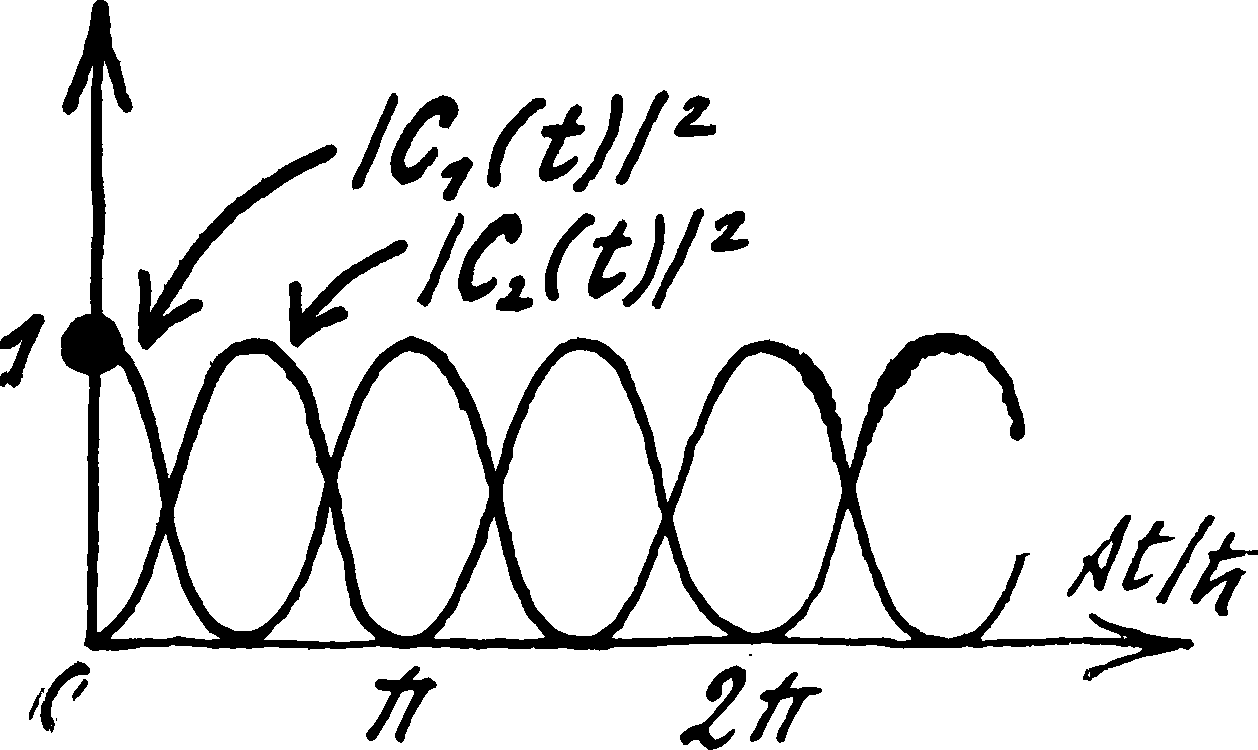
\includegraphics[width=\textwidth]{figures/fig-13-01.pdf}
\caption{Probability of microparticle remaining in different states as
given by equations \ref{eq-13.11}.}
\label{fig-13.1}
\end{marginfigure}

It is useful to compare (\ref{eq-13.5}) and (13.11). While in the first case the probabilities $|C_{1}|^{2}$ and  $|C_{2}|^{2}$ are invariant in time, their
dependence on time in the second case is quite obvious. The time
dependence of the probabilities  $|C_{1}(t)|^{2}$ and  $|C_{2}(t)|^{2}$
determined by relations (13.11.) is shown in Figure \ref{fig-13.1}.
\end{description}

Let \marginnote{Diagonalization of the Hamiltonian Matrix}us compare
the expressions for $C_{1} +C_{2}$ and $C_{1} - C_{2}$, obtained in
the previous section, with (\ref{eq-13.4}). This comparison allows us to
conclude that the amplitudes $C_{1} +C_{2}$ and $C_{1} - C_{2}$ describe the
stationary states of the microparticle with energies equal to $(E_{0} - A)$
and $(E_{0} - A)$, respectively. Further, we introduce a new pair of basic
states
\addtocounter{equation}{3}
\begin{equation}
\begin{split}
\bra{\mathrm{I}} & = \frac{1}{\sqrt{2}} \left( \bra{1} - \bra{2} \right)\\
\bra{\mathrm{II}} & = \frac{1}{\sqrt{2}} \left( \bra{1} + \bra{2} \right)
\end{split}
\label{eq-13.12}
\end{equation}

(it is easy to see that if the states $\bra{1}$ and $\bra{2}$ satisfy
the orthonormalization condition (\ref{eq-10.8}), the states
$\bra{\mathrm{I}}$ and $\bra{\mathrm{II}}$ also satisfy this
condition). By using (\ref{eq-13.12}), we rewrite (\ref{eq-13.1}) in the form
\begin{equation}
\bra{s} = \frac{C_{1}- C_{2}}{\sqrt{2}}\bra{\mathrm{I}} +  \frac{C_{1}+ C_{2}}{\sqrt{2}}\bra{\mathrm{II}} 
\label{eq-13.13}
\end{equation}

It can be seen from here that a transition from the basic states
$\bra{1}$ and $\bra{2}$ to the basic states $\bra{\mathrm{I}}$ and
$\bra{\mathrm{II}}$ corresponds to a transition from amplitudes
$C_{1}$ and $C_{2}$ to amplitudes $\left( \dfrac{C_{1} -
    C_{2}}{\sqrt{2}} \right)$
and $\left( \dfrac{C_{1} + C_{2}}{\sqrt{2}}\right)$. Since the latter describe the
stationary states of the microparticle, it follows that the transition
under consideration is associated with a diagonalization of the
Hamiltonian matrix.
\begin{equation*}
\begin{bmatrix}
E_{0} & -A \\
-A & E_{0} 
\end{bmatrix}
\to 
\begin{bmatrix}
E_{0}+A & 0 \\
0 & E_{0}-A
\end{bmatrix}
\end{equation*}

Thus, suppose we have a certain microparticle under certain external
conditions. Let us choose a certain system of basic states. The
attempt is usually made to choose basic states which have a clear
physical meaning (as we did, for example, in the case of the ammonia
molecule or the hydrogen molecule). The basic states chosen on the
basis of such considerations lead, in the general case, to a
Hamiltonian matrix whose non-diagonal elements are different from zero
(the microparticle undergoes transitions between the basic
states). Further, it is possible to go over to a new system of basic
states for which the Hamiltonian matrix is diagonal. The new basic
states describe the stationary states of the microparticle; the
elements of the diagonalized Hamiltonian matrix are essentially the
values of the energy in these states.


In the \marginnote{General Case}general case the non-diagonal elements
of the Hamiltonian matrix are different from zero and so the
simplifying conditions (\ref{eq-13.6}) and (\ref{eq-13.7}) are not
applicable. In this case one must solve not the simplified system of
equations (\ref{eq-13.8}), but the more general system of equations
(\ref{eq-13.2}) for a microparticle with two basic states. We suggest
that the reader, if he so desires, solves the system (\ref{eq-13.2})
himself, assuming for the sake of simplicity that the Hamiltonian
matrix is invariant in time\sidenote{Such a solution is given, for
  example, in Feynman. \cite{feynman-1965b}} We shall limit ourselves
here giving some results.

The energy of the stationary states of a microparticle is determined
by the expression
\begin{equation}%
E_{\mathrm{I, \, II}} = \frac{ H_{11}+H_{22}}{2} \pm \sqrt{\left( \frac{H_{11}-H_{22}}{2} \right)^{2}+H_{12}H_{21}}
\label{eq-13.14}
\end{equation}

The basic states $\bra{\mathrm{I}}$ and $\bra{\mathrm{II}}$
corresponding to these energy values are expressed in terms of the
elementary states $\bra{1}$ and $\bra{2}$ describing the equation
system (\ref{eq-13.2}) in the following manner:
\begin{equation}%
\left.
\begin{split}
\bra{\mathrm{I}} & = a_{1} \bra{1} + b_{1} \bra{2} \\
\bra{\mathrm{II}} & = a_{2} \bra{1} + b_{2} \bra{2}
\end{split}
\; \right\}
\label{eq-13.15}
\end{equation}
    where 
\begin{equation}%
\left.
\begin{split}
|a_{1}|^{2} + |b_{1}|^{2} & = |a_{2}|^{2} + |b_{2}|^{2} = 1\\
\frac{a_{1}}{b_{1}} & = \frac{H_{12}}{E_{\mathrm{I}} - H_{11}} \\
\frac{a_{2}}{b_{2}} & = \frac{H_{21}}{E_{\mathrm{II}} - H_{22}}
\end{split}
\; \right\}
\label{eq-13.16}
\end{equation}

It can be easily seen that if $H_{11} =H_{22} = E_{0}$ and $H_{12} =
H_{21} = - A$, the result (\ref{eq-13.14}) gives $E_{\mathrm{I, \,
    II}} = E_{0} \pm A$, the superpositions (\ref{eq-13.15}) turn into
(\ref{eq-13.12}). In other words, we arrive at the simplified case of the non-diagonal Hamiltonian matrix discussed above in detail. But if $H_{12} =
H_{21} = 0$, the result (\ref{eq-13.14}) gives $E_{\mathrm{I}} =
H_{11}, E_{\mathrm{II}} = H_{22}$ -- we arrive at
the case of the diagonal Hamiltonian matrix $\left( \bra{\mathrm{I}}
  =\bra{1}, \, \bra{\mathrm{II}} = \bra{2} \right)$

We \marginnote{Example of the Ammonia Molecule}recall that the basic
states $=\bra{1}$ and $=\bra{2}$ of the ammonia molecule were chosen
using graphic physical considerations: they correspond respectively to
the position of the nitrogen atom on one side of the $H$-plane and on
the other. Since these positions are symmetrical, we may take $H_{11}
= H_{22} \equiv E_{0}$. Assuming further that the elements $H_{12}$
and $H_{21}$ are real $(H_{12}= H_{21} \equiv -A$), which, as it turns
out, does not involve the loss of generality in this case, we arrive
at the. situation to which the simplified system of equation
(\ref{eq-13.8}) corresponds. It follows from this that the energy
levels of a molecule are essentially $E_{0} + A$ and $E_{0} - A$. We
emphasize that if no transitions took place between the states
$\bra{1}$ and $\bra{2}$, there would have been only one level $E_{0}$
in place of the levels $E_{0} + A$ and $E_{0} - A$. It would have been
doubly degenerate since there would be two states corresponding to
it. It may be said that transitions between the states $\bra{1}$ and $\bra{2}$
(associated with ``pushing'' of the nitrogen atom through the $H$-plane)
correspond to a removal of degeneracy, i.e. to a splitting of the level
$E_{0}$ into two levels $E_{0} + A$ and $E_{0} - A$.
     

Further, let us assume that the ammonia molecule is placed in a static
electric field with intensity $\Ea$ which is perpendicular to the
$H$-plane. Denoting the electric dipole moment of the molecule by $d$,
we write
\begin{equation}%
\begin{split}
H_{11}& = E_{0} + \Ea d \\
H_{22} & = E_{0} - \Ea d
\end{split}
\label{eq-13.17}
\end{equation}

Now the positions of the nitrogen atom on either side of the $H$-plane
are no longer physically symmetrical ($H_{11} \ne H_{22}$). Assuming
that $H_{12} =H_{21} = - A$ as before, we write the system of
equations (\ref{eq-13.2}) for the case under consideration:
\begin{marginfigure}%
\centering
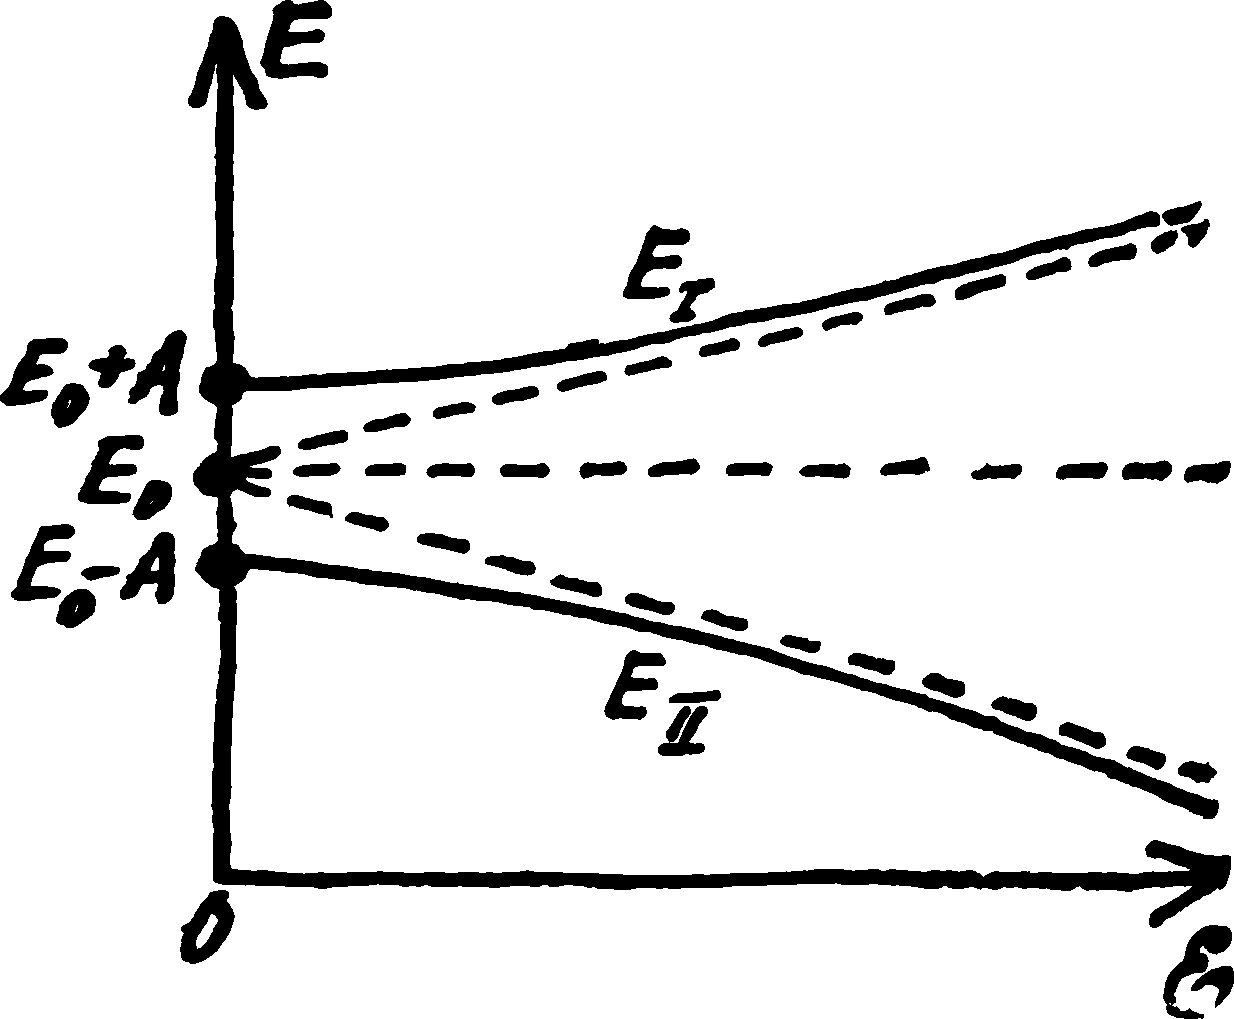
\includegraphics[width=\textwidth]{figures/fig-13-02.pdf}
\caption{Qualitative dependence of energy levels of ammonia molecule
  on the field intensity.}
\label{fig-13.2}
\end{marginfigure}

\begin{equation}%
\left.
\begin{split}
-i \hbar \frac{d}{dt} C_{1} & = (E_{0} + \Ea d )C_{1} - AC_{2}\\
-i \hbar \frac{d}{dt} C_{2} & = - AC_{1} + (E_{0} - \Ea d )C_{2}
\end{split}
\; \right\}
\label{eq-13.18}
\end{equation}

By using (\ref{eq-13.14}),we obtain the following expressions for the energy
Ievels of the molecule in a static electric field:

\begin{equation}%
\begin{split}
E_{\mathrm{I}} & = E_{0} + \sqrt{A^{2} + \Ea^{2} d^{2}} \\
E_{\mathrm{II}} & = E_{0} - \sqrt{A^{2} + \Ea^{2} d^{2}} 
\end{split}
\label{eq-13.19}
\end{equation}

Figure \ref{fig-13.2} shows the qualitative dependence of the energy levels of
ammonia molecule on the field intensity. It can be easily seen that,
the effect of ``throwing'' the nitrogen atom through the $H$-plane is
important for relatively small field intensities. In strong fields,
when the levels diverge considerably, this effect becomes
insignificant.


\section{The Electron in a Magnetic Field}
\label{sec-14}

It is well known that the projection of the electron spin momentum in
any direction may assume only two values $- \nicefrac{\hbar}{2}$ and
$+ \nicefrac{\hbar}{2}$. This allows us to treat the electron as a microparticle with two basic states. The problem of an electron in a magnetic field is of great practical interest. Besides, this problem is also quite interesting from a methodical point of view: its analysis enables one to get acquainted with not only the general nature of a system with two basic states, or, in other words, the two-level system, through a physically suggestive example, but also with the general approach to the analysis of such systems.

Let \marginnote{Hamiltonian Matrix for an Electron in a Magnetic
  Field} us first fix the direction of the coordinate axes (including
the direction of the $z$-axis). For the basic states $\bra{1}$ and
$\bra{2}$ we choose states for which the projections of the electron
spin on the $z$-axis are equal to $- \nicefrac{\hbar}{2}$ and $+
\nicefrac{\hbar}{2}$, respectively. We switch on a static magnetic
field (we denote the value of the magnetic induction by $B$) and
consider the following two cases.

\begin{description}[leftmargin=1cm]
\item[First case:] the magnetic field is directed along the $z$-axis
  ($B_{x} = B_{y} = 0$). In this case the basic states $\bra{1}$ and
  $\bra{2}$ are stationary; the state $\bra{1}$ has energy $- \mu
  B_{z}$ and the state $\bra{2}$ has energy $\mu B_{z}$ ($\mu$ denotes
  the magnetic moment of the electron). The amplitudes $C_{1}$ and $C_{2}$
  satisfy two independent equations of the type (\ref{eq-13.3}):
\begin{equation}%
\begin{split}
i \hbar \frac{d}{dt} C_{1} & = \mu B_{z} C_{1} \\
-i \hbar \frac{d}{dt} C_{2} & = \mu B_{z} C_{2} \\
\end{split}
\label{eq-14.1}
\end{equation}

The Hamiltonian matrix of the electron is of the form
\begin{equation}%
\begin{bmatrix}
H
\end{bmatrix}
=
\begin{bmatrix}
- \mu B_{z} & 0 \\
0 & \mu B_{z} \\
\end{bmatrix}
\label{eq-14.2}
\end{equation}



\item[Second case:] the magnetic field is in an arbitrary
  direction. In the first place, we note that irrespective of the
  direction of the field (in other words, irrespective of the choice
  of the direction of the coordinate axes) the energy levels of the
  electron are determined by the expressions $- \mu B$ and $ \mu B$;
  while in the previous case we had to take $B =B_{z}$, in this case
  we must have $B =\sqrt{B_{x}^{2}+ B_{y}^{2} + B_{z}^{2}}$. Thus
\begin{equation}%
\begin{split}
E_{\mathrm{I}} & = - \mu \sqrt{B_{x}^{2}+ B_{y}^{2} + B_{z}^{2}} \\
E_{\mathrm{II}} & = \mu \sqrt{B_{x}^{2}+ B_{y}^{2} + B_{z}^{2}} 
\end{split}
\label{eq-14.3}
\end{equation}
Note that
\begin{equation}%
E_{\mathrm{I}} = - E_{\mathrm{II}} 
\label{eq-14.4}
\end{equation}
\end{description}

Further we make use of relation (\ref{eq-13.14}). By taking
(\ref{eq-14.4}) into account, we may assume that $H_{11} + H_{22} = 0$. As a result, by combining (\ref{eq-14.3}) and (\ref{eq-12.9}), we get

\begin{equation}%
\left( \frac{H_{11} - H_{22}}{2}  \right)^{2} + |H_{12}|^{2} = \mu^{2}
\left( B_{x}^{2}+ B_{y}^{2} + B_{z}^{2} \right)
\label{eq-14.5}
\end{equation}


We shall assume a linear relationship between the elements of the
Hamiltonian matrix and the field. It turns out that this fairly
natural assumption allows us to derive the following relations from
(\ref{eq-14.5}): 
\begin{equation*}
\begin{split}
H_{11} & = - \mu B_{z},\\
H_{22} & = \mu B_{z},\\
H_{21} = H_{12}^{*} & = - \mu (B_{x} + iB_{y})
\end{split}
\end{equation*}
Thus, the Hamiltonian matrix of an electron in a magnetic field -has
the following general form:

\begin{equation}%
\begin{bmatrix}
H
\end{bmatrix}
=
\begin{bmatrix}
- \mu B_{z} & - \mu (B_{x} - iB_{y}) \\
- \mu (B_{x} + iB_{y})  & \mu B_{z} \\
\end{bmatrix}
\label{eq-14.6}
\end{equation}

It can be easily seen that when $B_{x} = B_{y} = 0$, the matrix (\ref{eq-14.6}), as
expected, coincides with the matrix (\ref{eq-14.2}). 

By using (\ref{eq-14.6}) we write the system of equation (\ref{eq-13.2}) for the case under consideration:

\begin{equation}%
\left.
\begin{split}
-i \hbar \frac{d}{dt} C_{1} & = - \mu \left[ B_{z} C_{1} + (B_{x} -
  iB_{y}) C_{2} \right] \\   
-i \hbar \frac{d}{dt} C_{2} & = - \mu \left[  (B_{x} +
  iB_{y}) C_{1} - B_{z} C_{2} \right]
\end{split}
\; \right\}
\label{eq-14.7}
\end{equation}


In conclusion, we note that although the above argument was conducted
for the case when the Hamiltonian matrix is invariant in time, the
results (\ref{eq-14.6}) and (\ref{eq-14.7}) are valid even when the
magnetic field varies with time. 

\begin{marginfigure}%
\centering
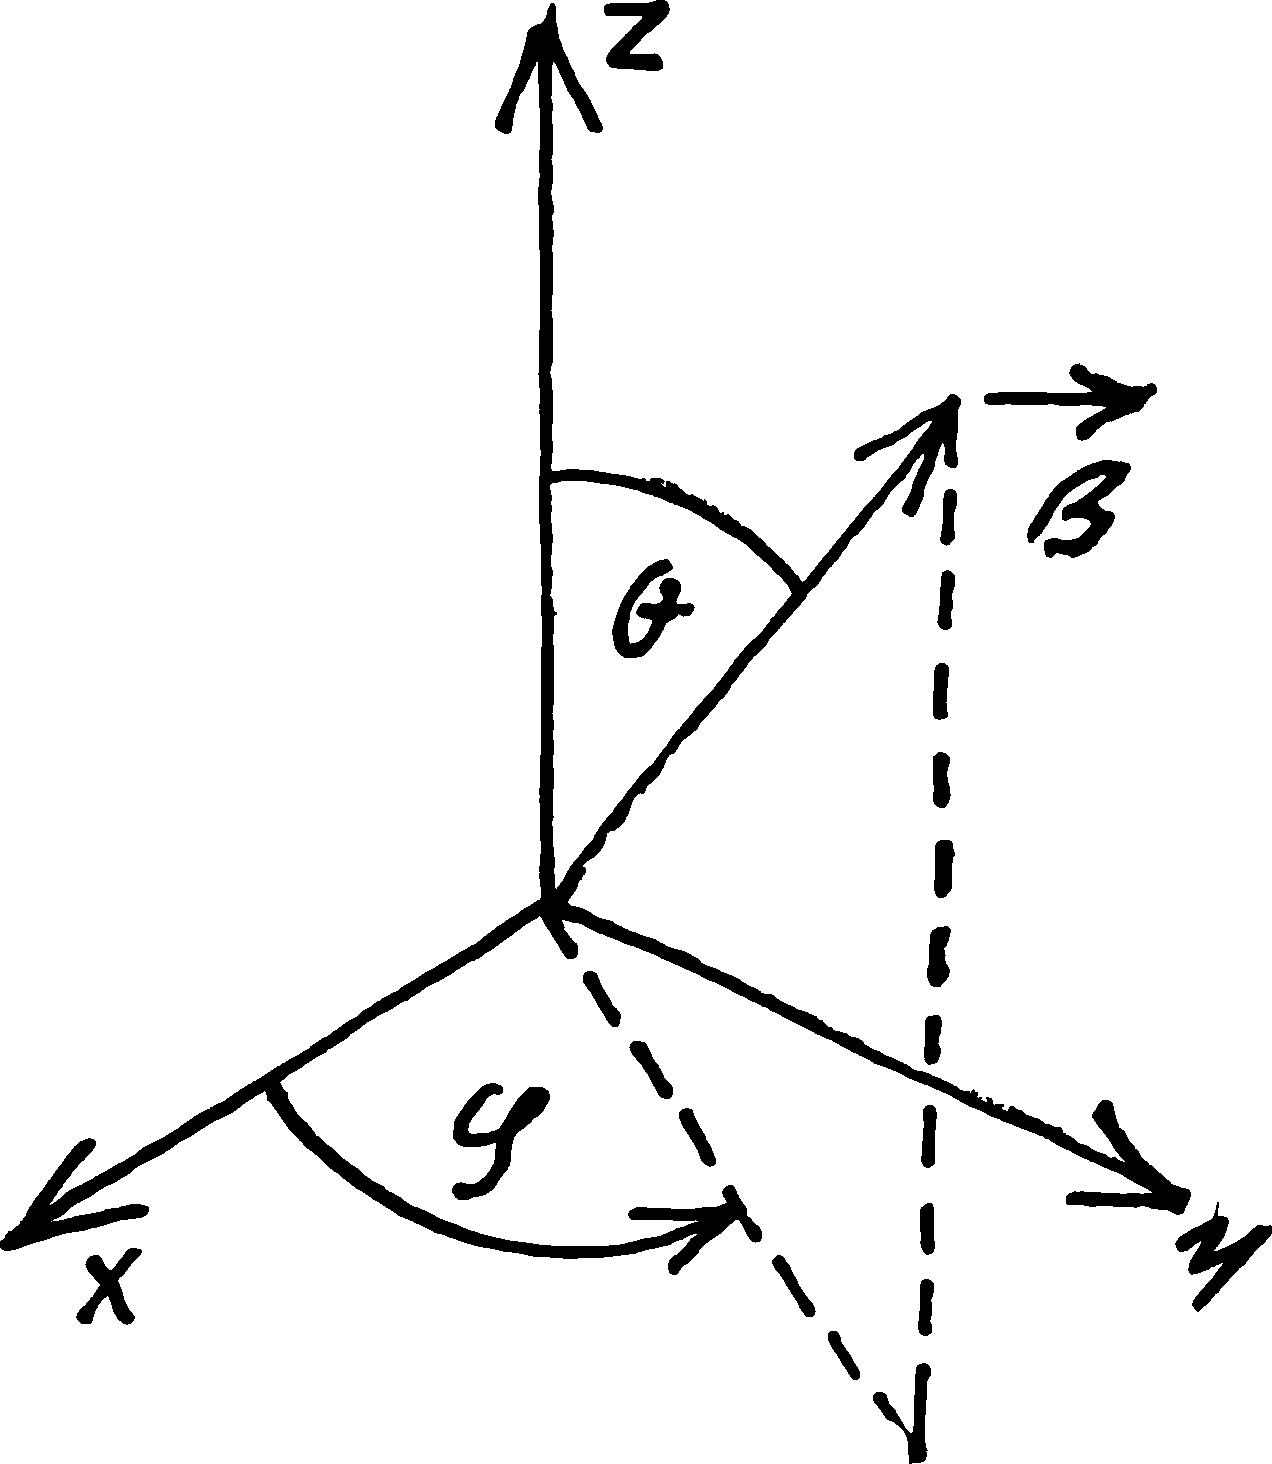
\includegraphics[width=\textwidth]{figures/fig-14-01.pdf}
\caption{Direction of the magnetic field.}
\label{fig-14.1}
\end{marginfigure}

Let \marginnote{Projection Amplitudes}the direction of the magnetic
field be determined by the polar angle $\theta$ and azimuth $\varphi$
(Figure \ref{fig-14.1}). We shall assume that the electron spin is
directed along the field; consequently, the electron is in the
stationary state $\bra{\mathrm{I}}$ with energy $E_{1} = - \mu B$. According to (\ref{eq-13.15}), the state $\bra{\mathrm{I}}$ can be represented as a superposition:

\begin{equation}%
\bra{\mathrm{I}} = a_{1} \bra{1} + b_{1} \bra{2}
\label{eq-14.8}
\end{equation}

where, as we recall, $\bra{1}$ and $\bra{2}$ are the states in which
the projections of the electron spin on the $z$-axis are equal to
$dfrac{\hbar}{2}$ and  $- dfrac{\hbar}{2}$, respectively, and the coefficients al and bi are determined by the relations (\ref{eq-13.16}):

\begin{equation}%
\begin{split}
& \frac{a_{1}}{b_{1}}  = \frac{H_{12}}{E_{\mathrm{I}} - H_{11}} \\
& |a_{1}|^{2} + |b_{1}|^{2}  = 1
\end{split}
\label{eq-14.9}
\end{equation}

By using (\ref{eq-14.6}) we write
\begin{equation}%
\left.
\begin{split}
H_{11} & = - \mu B_{z} = \mu B \cos \theta \\   
H_{12} & = - \mu (B_{x} - i B_{y}) = \mu B \sin \theta  \exp (- i \varphi)
\end{split}
\; \right\}
\label{eq-14.10}
\end{equation}
Substituting (\ref{eq-14.10}) into (\ref{eq-14.9}), we find that 

\begin{equation*}%
\frac{a_{1}}{b_{1}}  = \frac{ \sin \theta \exp ( - i \varphi) }{1 -
  \cos \theta}
\end{equation*}
Taking into account that $|a_{1}|^{2} + |b_{1}|^{2} = 1$, we arrive at
the following final result:

\begin{equation}%
\left.
\begin{split}
a_{1} & = \cos \left( \frac{\theta}{2} \right)  \exp \left( \frac{-i
    \varphi}{2} \right) \\   
b_{1} & = \sin \left( \frac{\theta}{2} \right)  \exp \left( \frac{i
    \varphi}{2} \right) 
\end{split}
\; \right\}
\label{eq-14.11}
\end{equation}

Thus, we have determined the amplitudes of the probabilities that the electron has its spin directed along the $z$-axis (amplitude $a_{1}$) or in the opposite direction (amplitude $b_{1}$) by assuming that the electron spin is directed along the field (i.e. in the direction determined by the angles $\theta$ and $\varphi$).

Note that (\ref{eq-14.11}) does not contain the magnetic induction
$B$. It is obvious that the result (\ref{eq-14.11}) must be valid in
the limiting case $B \to 0$. In other words we may exclude the field
from consideration and interpret (\ref{eq-14.11}) in the following
way. It is clear that the direction of the electron spin is determined
by the angles $\theta$ and $\varphi$. In this case the amplitude of
the probability that the electron spin is along the $z$-axis is $a_{1}$ and
the amplitude of the probability that the electron spin is in the
opposite direction is $b_{1}$. Expression (\ref{eq-14.8}) should be treated in this
case as an expansion of the spin state $\bra{\theta, \varphi}$ in terms of the spin
states $\bra{z}$ and  $\bra{-z}$: 

\begin{equation}%
\bra{\theta, \varphi}  = \cos \left( \frac{\theta}{2} \right) \exp
\left( - \frac{ i \varphi}{2} \right) \bra{z} + \sin \left( \frac{\theta}{2} \right) \exp
\left( \frac{ i \varphi}{2} \right) \bra{- z}  
\label{eq-14.12}
\end{equation}

The amplitudes of the states occurring in (\ref{eq-14.12})
\begin{equation}%
\begin{split}
\Braket{\theta , \varphi | z} & = \cos \left( \frac{\theta}{2} \right) \exp
\left( - \frac{ i \varphi}{2} \right) \\
\Braket{\theta , \varphi | -z} & = \sin \left( \frac{\theta}{2} \right) \exp
\left( \frac{ i \varphi}{2}  \right)
\end{split}
\label{eq-14.13}
\end{equation}

are called \emph{projection amplitudes}. 

By using projection amplitudes, we may predict the result of the
following experiment. Let an electron beam, polarized in a direction
given by the angles $\theta$ and $\varphi$, pass through some
``filter'' which only allows through electrons whose spin is along the
$z$-axis. In this case the amplitude of probability of an electron
passing through the apparatus (through the ``filter'') is
$\Braket{\theta, \varphi | z}$. The projection amplitude here plays
the role of the amplitude of the electron transition from the state
$\bra{\theta, \varphi}$ to the state $\bra{z}$.


Let \marginnote{Precession of the Electron Spin}the direction of the
electron spin be given by the angles $\theta$ and $\varphi$ (the
electron is in the state $\bra{\theta, \varphi}$). This state can be
represented in the form of superposition (\ref{eq-14.12}) of the
states $\bra{z}$ and $\bra{-z}$. Suppose that at time $t = 0$ we
switch on a magnetic field $B$ which is directed along the
$z$-axis. Now the states $\bra{z}$ and $\bra{-z}$ become stationary
states. Using this, we write [see (\ref{eq-13.4})]
\begin{equation}%
\left.
\begin{split}
\Braket{\theta, \varphi | z}  & = C_{1} \exp \left( \frac{-i \mu B_{z} t}{\hbar} \right) \\   
\Braket{\theta, \varphi | - z}  & = C_{2} \exp \left( \frac{i \mu B_{z} t}{\hbar} \right) 
\end{split}
\; \right\}
\label{eq-14.14}
\end{equation}
Comparing (\ref{eq-14.14}) with (\ref{eq-14.13}), we conclude that

\begin{equation}%
\left.
\begin{split}
C_{1}(0) & = \cos \left( \frac{\theta}{2} \right)  \exp \left( \frac{-i
    \varphi}{2} \right) \\   
C_{2}(0) & = \sin \left( \frac{\theta}{2} \right)  \exp \left( \frac{i
    \varphi}{2} \right) 
\end{split}
\; \right\}
\label{eq-14.15}
\end{equation}

It follows from this that in time $t$ after the magnetic field has been
switched on the projection amplitudes assume the form

\begin{equation}%
\left.
\begin{split}
\Braket{\theta, \varphi(t) | z}  & =  \cos \left( \frac{\theta}{2}
\right) \exp \left(-\frac{i}{2} \left( \varphi +  \frac{2 \mu B_{z}
      t}{\hbar} \right) \right) \\   
\Braket{\theta, \varphi(t) | - z}  & = \sin \left( \frac{\theta}{2} \right)  \exp \left(\frac{i}{2} \left( \varphi +  \frac{2 \mu B_{z}
      t}{\hbar} \right) \right)
\end{split}
\; \right\}
\label{eq-14.16}
\end{equation}

Thus, the switching on of a magnetic field along the $z$-axis does not
change the polar angle $\theta$ but changes the azimuth $\varphi$, the
change in $\varphi$ being proportional to the time interval $t$ which
elapses after switching on the field. This means that the spin of an
electron precesses around the $z$-axis (around the direction of magnetic
field) with a constant angular velocity. It can be easily seen that
the angular velocity of the spin precession is given by the relation
\begin{equation}%
\omega = \frac{2 \mu B_{z}}{\hbar} 
\label{eq-14.17}
\end{equation}

We move one step further by ignoring coordinate axes. Suppose that at
time $t = 0$ the direction of electron spin forms an angle $\theta$ with the
direction of the magnetic field. This angle will remain constant with
time, but the electron spin will precess around the field direction
with an angular velocity 

\begin{equation}%
\omega = \frac{2 \mu B}{\hbar} 
\tag{14.17a}
\label{eq-14.17a}
\end{equation}

We further suppose that the magnetic field is varying with time (in
the general case, both the direction and the magnitude of the vector
$\vec{B}$ are varying). A change in the field leads to a corresponding change
in the electron spin precession: a change in the magnitude of the
magnetic field results in a change in the angular velocity of
precession, while a change in the direction of the field causes a
change in the direction around which the precession takes place.
\begin{marginfigure}%
\centering
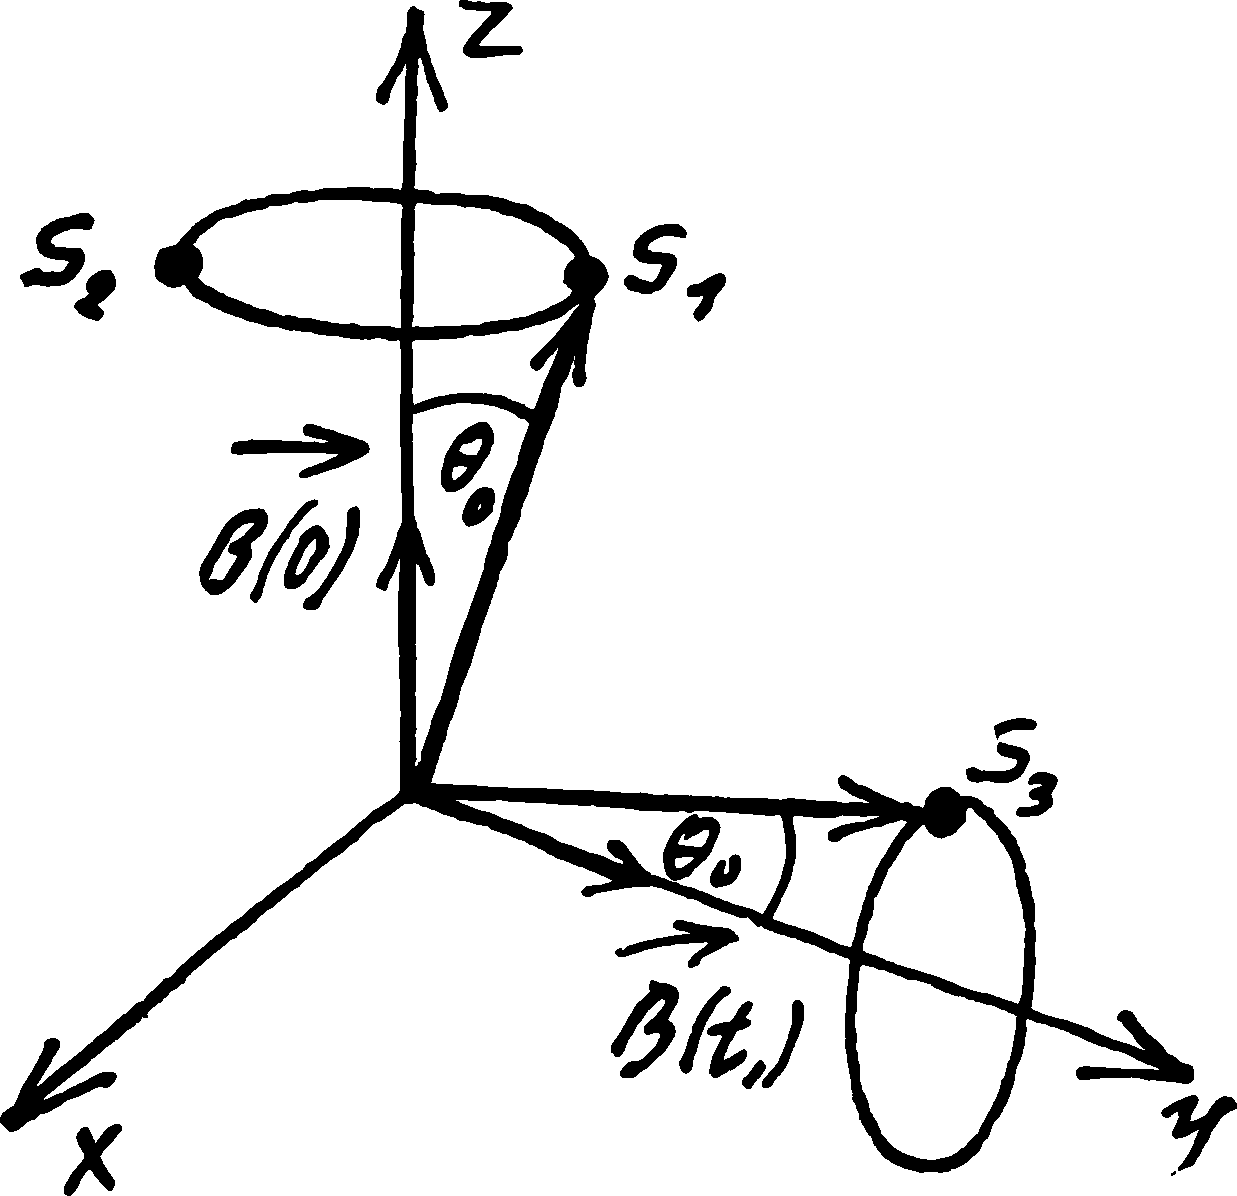
\includegraphics[width=\textwidth]{figures/fig-14-02.pdf}
\caption{A precessing of the magnetic field.}
\label{fig-14.2}
\end{marginfigure}

A knowledge of the precession enables one to predict changes in the
electronic state over a given period of time. We shall consider a
simple example (Figure \ref{fig-14.2}). Suppose that at the instant $t
= 0$ the field is directed along the $z$-axis [vector $\vec{B} (0)$],
and the electron spin is in the $zy$-plane and forms an angle
$\theta_{0}$ with the direction of the field. Thus the initial state
of the electron $\braket{ \theta(0), \varphi(0})$ is determined by the
angles $\theta (0) = \theta_{0}$ and $\varphi (0) = \dfrac{\pi}{2}$. We
shall assume that the magnitude of the field does not change with
time, but that the direction of the field changes. Suppose after time
$t_{1} = \dfrac{\pi \hbar}{2 \mu B}$ the field becomes directed along
the $y$-axis [vector $\vec{B}(t_{1})$ in Figure \ref{fig-14.2}]. What
will be the state of the electron at the $t_{1}$? It is clear that if
the field direction had remained unchanged, the end point of the
electron spin vector, while precessing around the $z$-axis, would have
described a semicircle during the time $\dfrac{\pi \hbar}{2 \mu B}$,
thus shifting from point $s_{1}$ to point $s_{2}$. If we take into
account the variation in field direction, we shall find that it has
shifted not to the point $s_{2}$ but to the point
$s_{3}$. Consequently, the required state of the electron
$\bra{\theta(t_{1}), \varphi (t_{1})}$ ) would be determined by the
angles 
\begin{equation*}%
\begin{split} 
\theta (t_{1}) & = \frac{\pi}{2} - \theta_{0}\\
\varphi (t_{1}) & = \frac{\pi}{2} 
\end{split}
\end{equation*}

According to \marginnote{Generalization of the Problem of an Electron in
a Magnetic Field to an Arbitrary Two-Level System} Feynman, \emph{it
is interesting that the mathematical ideas we have just gone over for
the spinning electron in a magnetic field can be applied to any two-
state system. That means that by making a mathematical analogy to the
spinning electron, any problem about two- state systems can be solved
by pure geometry \ldots If we can solve the electron problem in general,
we have solved all two-state problems.}\cite{feynman1965b} Let us clarify these remarks.


We shall consider some two-level system with the basic states
$\bra{1}$ and $\bra{2}$. We assign some vector to each state of the
microparticle. A choice of the basic states $\bra{1}$ and $\bra{2}$ in
this case is equivalent to a choice of the $z$-axis (as if these two
states correspond to the two $z$-projections of the electron
spin). Suppose that the microparticle is in the state  $\bra{s(0)}$ at
the initial moment of time. We assign to this state a vector whose
direction is determined by the angles $\theta (0)$ and $\varphi (0)$:
\begin{equation}%
\bra{s(0)} \leftrightarrow \bra{\theta(0), \varphi (0)} 
\label{eq-14.18}
\end{equation}

In order to find the angles $\theta (0)$ and $\varphi (0)$ we must expand the state
 $\bra{s (0)}$ in terms of the basic states  $\bra{1}$ and $\bra{2}$ and use for the
coefficients of expansion expression (\ref{eq-14.13}) for the projection
amplitudes. This expansion is of the form


\begin{equation}%
\bra{s(0)}  = \cos \left( \frac{\theta (0)}{2} \right) \exp
\left( - \frac{ i \varphi(0)}{2} \right) \bra{1} + \sin \left( \frac{\theta(0)}{2} \right) \exp
\left( \frac{ i \varphi(0)}{2} \right) \bra{2}  
\label{eq-14.19}
\end{equation}

Further, let us turn to the Hamiltonian matrix of the
microparticle. First of all we shift the zero point of the energy in
such a way that it is located precisely half-way between the two
energy levels or, in other words, so that the condition (\ref{eq-14.4}) is
satisfied. In this case
\begin{equation}%
H_{11}+ H_{22} = 0
\label{eq-14.20} 
\end{equation}
We now formally introduce a vector $\mu \vec{B}$ (it is in no way associated with
any magnetic field!) such that its projections on the coordinate
axes (remember that the axes are determined by the choice of the basic
states) satisfy the conditions
\begin{equation}%
\begin{split}
H_{11} & = - \mu B_{z}\\
H_{22} & = - \mu (B_{x} - i B_{y})
\end{split}
\label{eq-14.21} 
\end{equation}

By using (\ref{eq-14.21}) we determine 
\begin{equation}%
\omega =  \frac{2 \mu \sqrt{B_{x}^{2}+ B_{y}^{2} + B_{z}^{2}}}{\hbar}
\label{eq-14.22} 
\end{equation}

In order to solve this two-level problem, i.e. in order to determine
the change in the $\bra{s}$ state during certain time $t$, we must
consider the precession of the vector $\bra{\theta, \varphi}$ around
the direction $\vec{B}$ with an angular velocity $\omega$. If the
Hamiltonian matrix is time dependent, both the direction of $\vec{B}$ and the
magnitude of the angular velocity of precession will change
accordingly. After a time $t$, the microparticle will be in the state $\bra{s(t)}$ defined by the angles $\theta(t)$ and $\varphi (t)$, which may be determined
if we know the initial values $\theta(0)$ and $\varphi (0)$ and the precession (in
exactly the same way as was done in the example given at the end of
the preceding subsection). The transition from the angles $\theta(t)$
and $\varphi (t)$ to the required final state  $\bra{s(t)}$ is accomplished by using
the familiar superposition:
\begin{equation}%
\bra{s(t)}  = \cos \left( \frac{\theta (t)}{2} \right) \exp
\left( - \frac{ i \varphi(t)}{2} \right) \bra{1} + \sin \left( \frac{\theta(t)}{2} \right) \exp
\left( \frac{ i \varphi(t)}{2} \right) \bra{2}  
\label{eq-14.23}
\end{equation}


Applying these remarks to the example of the ammonia molecule
considered in Section \ref{sec-13}, we must shift the zero point of
the energy by an amount $E_{0}$, and go over (for the sake of
convenience) from the basic states $\bra{1}$ and $\bra{2}$ to the
basic states $\bra{\mathrm{I}}$ and $\bra{\mathrm{II}}$. As a result, we get in place of
(\ref{eq-13.18}) the following system of equations:
\begin{equation}%
\left.
\begin{split}
-i \hbar \frac{d}{dt} C_{\mathrm{I}} & = - A C_{\mathrm{I}} + \Ea d C_{\mathrm{II}} \\   
-i \hbar \frac{d}{dt} C_{\mathrm{II}} & = - \Ea d C_{\mathrm{I}} + A C_{\mathrm{II}} 
\end{split}
\; \right\}
\label{eq-14.24}
\end{equation}

This system is convenient for drawing the analogy with the electron in
a magnetic field. Comparing (\ref{eq-14.24}) and (\ref{eq-14.7}), we
find that the quantity $A$ corresponds to $- \mu B_{z}$ and the
quantity $\Ea d$ to $- \mu B_{x}$· Consequently, we have to consider
the precession of the vector describing the state $\bra{s}$ of the
molecule in the ``magnetic field'' which is made up of two components:
a constant component along the $z$-axis, associated with the effect of
the ``throwing'' of a nitrogen atom through the $H$-plane, and a component along the $z$-axis, associated with the electric field. The
latter component may, obviously, vary with time.\\[8pt]

\textsc{Pauli Spin Matrices}\\[5pt]
{\small In conclusion, we shall mention the \emph{Pauli spin
    matrices} which are widely used in the quantum mechanics of
  two-level systems. These matrices are of the form}
\begin{equation}%
\sigma^{x}= 
\begin{bmatrix}
0 & 1 \\
1 & 0
\end{bmatrix}
\;\;\; 
\sigma^{y}= 
\begin{bmatrix}
0 & -i \\
i & 0
\end{bmatrix}
\;\;\;
\sigma^{z}= 
\begin{bmatrix}
1 & 0 \\
0 & 1
\end{bmatrix}
\label{eq-14.25}
\end{equation}

{\small By using these matrices, we can rewrite the expression
for the elements of Hamiltonian matrix of all electron in a magnetic
fiald (\ref{eq-14.6}) in the following form: }
\begin{equation}%
H_{ij} = - \mu \left( \sigma^{x}_{ij}B_{x} + \sigma^{y}_{ij}B_{y}
  +\sigma^{z}_{ij}B_{z} \right)
\label{eq-14.26}
\end{equation}
{\small By considering $\sigma^{x}, \sigma^{y}, \sigma^{z}$ as components of
  some matrix vector $\vec{\sigma}$. we can rewrite (\ref{eq-14.26}) in a form which is independent of the choice of the coordinate axes: }

\begin{equation}%
H_{ij} = - \mu \vec{\sigma}_{ij} \vec{B}
\label{eq-14.27}
\end{equation}

{\small Pauli spin matrices are useful because any second-order
  matrix (in particular, the Hamiltonian matrix of any microparticle
  with two basic states) may be represented as a superposition of
  these matrices. The Pauli spin matrices introduced for an electron
  in a magnetic field have proved to be convenient for considering a
  wide range of two-level problems. This is not surprising when we
  consider the possibility, discussed above, of generalizing the
  problem of an electron in a magnetic field to arbitrary two-level
  systems.  }

\section{The Wave Function}
\label{sec-15}
At the very outset, let us make it clear that this section hardly adds
anything new to the physical foundations of quantum mechanics
considered in this chapter. In fact, we are already able to summarize
the physical aspects of the theory and go over to its mathematical
side, based on the use of linear operators. However, before doing so,
it is worthwhile to introduce the concept of the \emph{wave
  function}. Wave functions are widely used in the existing literature
on quantum mechanics; hence it is important that the reader should be
aware of the ``position'' of the wave function in the above description
of amplitude concepts. Until now, the wave function, being essentially
the amplitude of state, existed in this picture in an implicit form;
we shall now make it explicit. Besides, one must remember that while
changing over to the mathematical apparatus of quantum mechanics, it
is more convenient to use the wave function rather than the amplitude
of state.  

Let \marginnote{The Wave Function as the Amplitude of State }
$\bra{x}$ be the state of a microparticle corresponding to its
localization at a point in space with the coordinate $x$ (for
simplicity we consider the \emph{one-dimensional} case). Then
$\braket{s |x}$ may be considered as the probability amplitude that
a microparticle in the state $\bra{s}$ has the coordinate $x$.

However, we must make this a little more precise. When considering the
probability of any spatial localization of a microparticle, we must
take into account the continuity in the variation of a spatial
coordinate. Hence, instead of the probability of finding a
microparticle precisely at the point $x$, we must consider the
probability of finding it on the interval from $x$ to $x + dx$. Denoting
this probability by $dw_{s} (x)$, we have
\begin{equation}%
dw_{s} (x) = |\braket{s|x}|^{2} dx
\label{eq-15.1}
\end{equation}

Consequently, the quantity $\braket{s|x}$ is, strictly speaking, not the
amplitude of probability, but the \emph{amplitude of probability density}.

In literature, the quantitY $\braket{s|x}$ is referred to as the \emph{wave
function} and is expressed, for example, by $\psi_{s} (x)$. Thus,
\begin{equation}%
\psi_{s} (x) = \braket{s|x} 
\label{eq-15.2}
\end{equation}
Using (\ref{eq-15.2}) we can rewrite (\ref{eq-15.1}) as
\begin{equation}%
dw_{s} (x) = |\psi_{s}(x)|^{2} dx
\label{eq-15.3}
\end{equation}

It follows from (\ref{eq-15.3}) that $ |\psi_{s}(x)|^{2}$ is the
probability density of finding a microparticle with the state $\bra{s}$ at the point $x$. 

From a mathematical point of view, the wave function in $\psi_{s}(x)$
is a \emph{parametric function}, the parameters being the quantities which
are precisely defined in the state $\bra{s}$. Taking into account the
earlier remarks on the structure of amplitudes of states, we may state
that the quantities of one complete set serve as the \emph{argument} for the
wave function, its parameter being the quantities of another set. It
is often said that the wave function $\psi_{s}(x)$ is an \emph{eigenfunction} of
the quantities of the $s$-set, given in the representation determined
by the quantities of the $x$-set (or simply, in the $x$-representation).


Wave \marginnote{Generalization of the Concept of The Wave Function}
functions are frequently used in practice in the $x$-representation
(\emph{coordinate representation}). However  apart from the
$x$-representation, other representations are obviously also
possible. In this connection, the concept of the wave function must be
generalized: 
\begin{equation}%
\psi_{a} (\beta) = \braket{\alpha | \beta}
\label{eq-15.4} 
\end{equation}
The function $\psi_{a} (\beta) $ is the eigenfunction of the
quantities of the $\alpha$-set, given in the
$\beta$-representation. If the values of the $\beta$-set change
discretely, $\psi_{a} (\beta) $ is the amplitude of the probability
that the state $\bra{\beta}$ is represented in the state
$\bra{\alpha}$. In the case of continuously changing values of the
$\beta$-set, $\psi_{a} (\beta)$ is the amplitude of the given
probability density.

By giving the wave function $\psi_{a} (\beta) $ we give the exact
values of the quantities in the $\alpha$-set and probable values of
the quantities in the $\beta$-set. Correspondingly, by giving the
function $\varphi_{a} (\gamma) $ we give the exact values of the
$\alpha$-set and probable for the values of the $\gamma$-set. It could
be said that the function $\psi_{a} (\beta) $ describes the state
$\bra{\alpha}$ in the $\beta$-representation, while the function
$\varphi_{a} (\gamma)$ describes the same state, but in the
$\gamma$-representation. The fact that different functions $\psi_{a}
(\beta)$ and $\varphi_{a} (\gamma)$ are used for describing the same
state $\bra{\alpha}$ , indicates that there must be some connection
between them. This connection is expressed through the \emph{principle
  of superposition of states}.  Assuming that $\gamma$-values change
discretely, we can write 

\begin{equation}%
\psi_{a} (\beta) = \sum_{i} \varphi_{a} (\gamma_{i}) \chi_{\gamma i} (\beta)
\label{eq-15.5}
\end{equation}

It can be easily seen that (\ref{eq-15.5}) is the expression for the
 superposition of amplitudes of states:
\begin{equation}%
\braket{\alpha | \beta} = \sum_{i}\braket{\alpha | \gamma_{i}}\braket{\gamma_{i} | \beta}
\tag{15.5a}
\label{eq-15.5a}
\end{equation}
If the $\gamma$-values vary continuously, we get in place of
(\ref{eq-15.5}) 
\begin{equation}%
\psi_{a} (\beta) = \int \varphi_{a} (\gamma) \chi_{\gamma} (\beta) d \gamma
\label{eq-15.6}
\end{equation}
Let us consider the eigenfunction of the quantities of a certain set
given in the representation of the quantities of the same set. If
these quantities change discretely, we have, according to
(\ref{eq-10.8}),
\begin{equation}%
\psi_{a_{i}} (\alpha_{j}) = \delta_{ij}
\label{eq-15.7}
\end{equation}
If, however, the quantities vary continuously, we get in place of (\ref{eq-15.7}) 
\begin{equation}%
\psi_{\alpha'} (\alpha) = \delta (\alpha - \alpha')
\label{eq-15.8}
\end{equation}
where $\delta (\alpha - \alpha')$ is the so-called \emph{Dirac delta
function}, which is a generalization of the Kronecker's symbol for the
case of continuously varying quantities.\sidenote{The delta function is
discussed in detail, for example, in \cite{schiff-1968}.}

The delta function is determined in the following
\begin{equation}%
\begin{split}
& \delta (\alpha - \alpha') = 0 \;\; \textrm{at} \;\; \alpha \ne
\alpha'\\
& \int\limits_{-\infty}^\infty \delta (\alpha - \alpha') d \alpha = 1
 \end{split}
\label{eq-15.9} 
\end{equation}
Strictly speaking, it is impossible to plot the function $\delta
(\alpha - \alpha')$ because it would involve drawing an infinitely
narrow and infinitely high peak at the point $\alpha = \alpha'$ with a
finite ``area'' under it equal to unity. One of the most important
properties of the delta function, which can be easily derived from its
definition (\ref{eq-15.9}), can be written as follows:
\begin{equation}%
\int\limits_{-\infty}^\infty f (\alpha) \delta (\alpha - \alpha') d
\alpha = f (\alpha ')
\label{eq-15.10}
\end{equation}
where $f (\alpha)$ is a bounded function, continuous at the point
$\alpha = \alpha'$. 

Assuming \marginnote{Condition of Orthonormalization of Eigenfunctions
}that the $\alpha$-values are discrete and the $\beta$-values vary
continuously we rewrite (\ref{eq-15.6}) in the form of
\begin{equation}%
\Psi_{\alpha_{i}}(\alpha_{j}) = \int \psi_{\alpha_{i}} (\beta)
\Phi_{\beta} (\alpha_{j})  d \beta
\label{eq-15.11}
\end{equation}
By using \ref{eq-9.33} we can write
\begin{equation}%
\Phi_{\beta} (\alpha_{j}) = \psi_{\alpha_{j}}^{*} (\beta)
\label{eq-15.12}
\end{equation}

From (\ref{eq-15.12}) and (\ref{eq-15.7}), we obtain from (\ref{eq-15.11}) the condition
for the orthonormalization of the eigenfunctions $\psi_{\alpha_{i}}(\beta)$
\begin{equation}%
\int \psi_{\alpha_{i}}(\beta) \psi_{\alpha_{j}}^{*} (\beta) d \beta = \delta_{ij}
\label{eq-15.13}
\end{equation}

If the $\alpha$-quantities vary continuously, we must use (\ref{eq-15.8}) instead of
(\ref{eq-15.7}). In this case the condition of orthonormalization of the
eigenfunctions assumes the form
\begin{equation}%
\int \psi_{\alpha}(\beta) \psi_{\alpha}^{*} (\beta) d \beta = \delta
(\alpha - \alpha')
\label{eq-15.14}
\end{equation}


As an \marginnote{The Wave Function of a Freely Moving Microparticle}
example, we consider the case of a freely moving microparticle. For
simplicity, we assume that it has zero spin. The wave function in
coordinate (three-dimensional) representation has the form\sidenote{We
  shall derive this result later (see Section \ref{sec-20}).}
\begin{equation}%
\begin{split}
 \psi_{\vec{p}_{0}} (\vec{r}) & = \Braket{\vec{p}_{0}| \vec{r}} \\
& = (2 \pi \hbar)^{-\frac{3}{2}} \exp \left( \frac{ i \vec{p}_{0} \vec{r}}{\hbar} \right)
\end{split}
\label{eq-15.15}
\end{equation}

where $\vec{p_{0}}$ is the momentum of the microparticle and $\vec{r}$
is its spatial coordinate. The function $ \psi_{\vec{p}_{0}}
(\vec{r})$ is an eigenfunction of the momentum, given in the
coordinate representation. It describes the state in which the
momentum components of a microparticle have definite values, while the
spatial coordinates may be assigned only probable values.

\begin{marginfigure}%
\centering
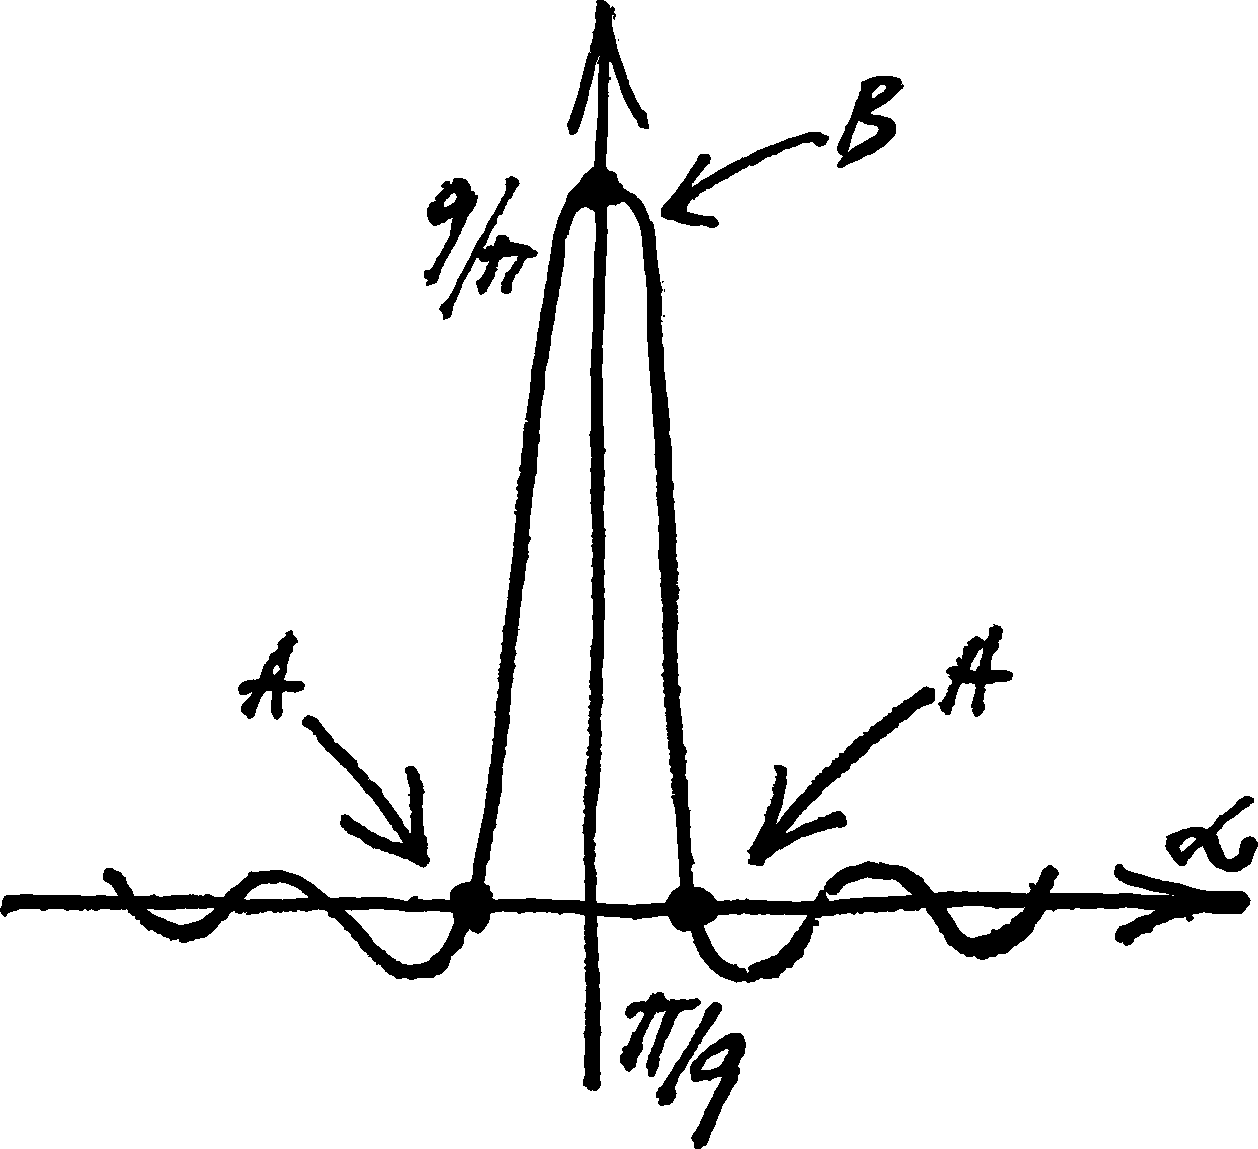
\includegraphics[width=\textwidth]{figures/fig-15-01.pdf}
\caption{The so called sinc function $\dfrac{\sin x }{x}$.}
\label{fig-15.1}
\end{marginfigure}

Switching over from the \emph{coordinate} to the \emph{momentum}
representation and making use of (\ref{eq-9.33}) we get 

\begin{equation}%
\begin{split}
 \varphi_{\vec{r}_{0}} (\vec{p}) & = \Braket{\vec{r}_{0}| \vec{p}}  = \Braket{\vec{p}| \vec{r}_{0}}^{*} \\
& = (2 \pi \hbar)^{-\frac{3}{2}} \exp \left(- \frac{ i \vec{r}_{0} \vec{p}}{\hbar} \right)
\end{split}
\label{eq-15.16}
\end{equation}

The function $\varphi_{\vec{r}_{0}} (\vec{p})$ is an eigenfunction of
the coordinate To of the microparticle given in the momentum
representation.


It can be seen from (\ref{eq-15.15}) and (\ref{eq-15.16}) that the states of a freely
moving microparticle are described by wave functions in the form of
\emph{plane waves} (in coordinate or momentum space).


The functions $\psi_{\vec{p}_{0}} (\vec{r})$ and
$\varphi_{\vec{r}_{0}} (\vec{p})$ satisfy the condition
(\ref{eq-15.14}) of orthonormalization. This can be verified by using
the integral representation of the delta function\sidenote[][-3.5cm]{Let
  us consider the function $\dfrac{\sin (g\alpha)}{\pi \alpha}$
  (Figure \ref{fig-15.1}). Irrespective of the value of parameter $g$,
  $\int\limits_{-\infty}^\infty d \alpha \dfrac{\sin (g\alpha)}{\pi
    \alpha} = 1$. Let us increase $g$. This will bring the points $A$
  in the figure closer to $\alpha = 0$, and raise the point $B$ on the
  ordinate axis. In the limit as $g \to \infty$ we get an infinitely
  narrow and high peak whose integral is equal to unity. This is just
  the delta function. Thus, $\delta (\alpha) = \lim\limits_{g \to \infty}
  \dfrac{\sin (g\alpha)}{\pi \alpha}$. We can easily get (\ref{eq-15.17}) from
  this since$\dfrac{\sin (g\alpha)}{\pi \alpha}  = \dfrac{1}{2 \pi} \int\limits_{-\infty}^\infty \exp (i \alpha \beta) d \beta$
}

\begin{equation}%
\delta (\alpha) = \frac{1}{2 \pi} \int\limits_{-\infty}^\infty \exp (i \alpha \beta) d \beta
\label{eq-15.17}
\end{equation}

(the quantities $\alpha$ and $\beta$ represent the components of the spatial
coordinate and the momentum of the microparticle).




\section{Quantum Mechanics as a Qualitative Leap in Man's Knowledge of
  the Laws of Nature}
\label{sec-16}
\vspace*{10pt}
\begin{fullwidth}
\begin{verse}
  \texttt{\small Of course it is impossible to distinguish sharply
    between \\
    natural philosophy and human culture. The physical sciences \\
    are, in fact, an integral part of our civilization, not only \\
    because  our ever-increasing mastery of the forces of nature \\
    has so completely changed the material conditions of life, \\
    but also because the study of these sciences has contributed \\
    so much to clarity the background of our own existence.}\\[8pt]

\texttt{\small \hspace{11cm}N. Bohr}

\end{verse}
\end{fullwidth}

Although quantum mechanics deals with microparticles, its significance is by no means limited to microphenomena. In our endless quest for understanding and perfecting our knowledge of the laws of nature, quantum mechanics represents an important qualitative leap. Without a comprehension of the importance, and radical (we could even say revolutionary) nature of this leap, it is impossible to understand the modern physical picture of the world. In this section, an attempt has been made to look at quantum mechanics from this point of view. This may serve as a logical conclusion to the chapter, which has been devoted to the physical foundations of this astonishing theory.


The \marginnote{``Crazy Idea''}expression ``crazy theory'' as one
which is ``crazy enough to be true'' was once coined by Bohr. This
expression reflects the stunning impression produced on Bohr's
contemporaries by the astonishing physical discoveries made at the
beginning of the 20$^{\mathrm{th}}$ century, discoveries which could not be
confined within the framework of classical concepts. It became
obvious that an explanation of these discoveries required radically
new ideas and a new approach.


In Section \ref{sec-02} we considered two fundamental ideas of quantum
mechanics-the idea at discreteness and the idea of duality. Returning,
in our imagination, to the beginning of the century, we could call the
first idea ``incomprehensible'' and the second, ``not properly
understood''. The introduction of discreteness to the physical picture
of the world led to incomprehensible and, apparently, logically
controversial quantum ``jumps'' The idea of duality, which asserts the
specific nature of microparticles, eliminated the contradiction of
quantum ``jumps'' by suggesting a ``manoeuvring'' between the
``particle'' and the ``wave'' concepts. But the meaning of the wave
concept introduced here remained in fact unclear for a very long
time. These two ``absurd'' ideas led to the emergence of the
extravagant ``ncertainty relations'' which resulted in a different
outlook on even such fundamental concepts as ``energy'', ``momentum''
and ``angular momentum''.


Quantum mechanics was born under circumstances of a significant breaking up of physical traditions. It called for a rejection of many usual and accepted notions such as the strict continuity of the spectra of values of physical quantities, the trajectory as an essential attribute of the motion of an object, Laplace determinism as the basic form of expression of the principle of causality, the possibility of an infinite detailization of the structure of an object or of a phenomenon with respect to time, the possibility of distinguishing between two objects, however similar to each other, under any circumstances, the belief that it is always possible, at least in principle, to disregard the measuring instrument when conducting any measurements, etc. (all these questions have been analysed in detail in the preceding sections).


It is difficult to recall any other period in the history of physics
when such a serious and large-scale revision of physical concepts was
carried out. According to Bohr, \emph{\ldots the new lesson which has
  been impressed upon physicists stresses the caution with which all
  usual conventions must be applied as soon as we are not concerned
  with everyday experience \ldots In the study of atomic phenomena we have repeatedly been taught that questions which were believed to have received long ago their final answers had most unexpected surprises in store for us.}

The \marginnote{The Essence of Quantum Mechanics} revision of the
concepts and the rejection of many accepted notions could well be
considered as a ``negative aspect'' of quantum mechanics. Let us now
consider its ``positive aspect''.


If we try to summarize the main positive knowledge imparted by
quantum mechanics to man in his search for learning about his
surroundings, the following two important points stand out:

\begin{description}[leftmargin=1cm]
\item[First:] quantum mechanics showed that the \emph{basic laws of nature
  are not dynamic but are statistical}, and that the \emph{probabilistic form
  0/causality is the fundamental form while the classical} determinism
  is just its limiting (degenerate) case.


\item[Second:] quantum mechanics revealed that \emph{probability in
    nature should not be dealt with as in classical statistical
    theories}. It was found that in certain cases it is not the
  probabilities of events that should be summed, but rather the
  amplitudes of these probabilities. This leads to the
  \emph{interference of probability amplitudes}.
\end{description}

Thus we emphasize firstly the \emph{probabilistic character of the laws of
nature} (the pre-eminence of statistical laws) and, secondly, the
\emph{special relations among the probabilities}, which assume not only the
summation of the latter, but also the specific interference
effects. In our view, it is in this that the main importance of the
information one gets from quantum mechanics is to be found.


As Born pointed out in \emph{Physics in my
  generation},\cite{born-1956} the statistical methods found wider
applicability with the development of physics. As regards modern
physics, it is completely based on statistical foundations. In Born's
view, it is the quantum theory that established the closest links
between statistics and the basic aspects of physics. This should be
considered as an important event in the history of human knowledge,
with consequences reaching far beyond the limits of science. It is
sometimes said that the fundamental difference between quantum
mechanics and classical mechanics is determined by, the statistical
nature of the former and dynamic nature of the latter. Upon careful
consideration, this apparently bland and irrefutable statement turns
out to be incorrect. While revealing the pre-eminence of statistical
laws in physics, quantum mechanics shows at the same time that dynamic
laws with their unique predictions are, as a matter of fact, a special
(degenerate) case of probability laws. In this respect not only
quantum mechanics, but classical mechanics as well, must be, strictly
speaking, formulated in the language of probabilities\sidenote{This
  point of view is systematically analysed by Myakishev
  \cite{myakishev-1973} where it is stated, in particular, that
  Feynman's concepts of path integrals in fact converts the principle
  of least action into the principle of maximum probability, i.e, it
  proves that the fundamental dynamic principle is essentially
  statistical in nature.} The qualitative difference between quantum
mechanics and classical mechanics (or classical physics in general)
depends on how the relations among probabilities are considered. It
has been mentioned in Mayakishev the main difference between quantum
mechanics and classical mechanics does not lie in the statistical
nature of the former. It lies in the fact that it is not the
probability but its amplitude, the wave function, that is of primary
importance in quantum mechanics. This leads to the interference of
probabilities, an effect which does not have an analogy in classical
mechanics.


Developing the above ideas, let us single out the following points:
\begin{enumerate}[label=(\alph*),leftmargin=1cm]
\item  the special interrelations among quantum-mechanical states and
the resulting specific nature of quantum-mechanical description of
phenomena;
\item the specific nature of the application of probabilities in quantum mechanics;
\item the special role of interference in quantum mechanics;
\item the complementarity principle as a logical foundation of quantum mechanics, and
\item the dialectical nature of quantum mechanics. We shall consider
  these questions one by one.
\end{enumerate}


According \marginnote{The Specific Nature of Quantum-Mechanical Description of Phenomena}to Feynman, one of the most outstanding achievements of
quantum mechanics lies in the fact that it allows so much to be
extracted from so little.


The reader has already found out how much can be achieved from the
phenomenon of interference of amplitudes (see Section \ref{sec-9}), on
the basis of the principle of superposition of states (see Section
\ref{sec-10}), and from a consideration of the simplest
quantum-mechanical systems, i.e, microparticles with two basic states
(see Sections. \ref{sec-13}, \ref{sec-14}). The relative formal
simplicity of the description of microphenomena is connected with the
specific nature of this description. Remember that for a
quantum-mechanical description we must know firstly the basic states
and, secondly, the Hamiltonian matrix, which reflects the physics of
the phenomena under consideration. A simplification in the description
can be achieved because of the following two circumstances.

\begin{description}[leftmargin=1cm]
\item[Firstly,] it is important that the number of basic states, and
  consequently the number of elements of the Hamiltonian matrix
  required for describing a definite phenomenon, should not be
  large. Thus, in the examples given in Sections \ref{sec-13} and
  \ref{sec-14}, this number was equal to two. Here the contradiction
  regarding the diversity in the possible states of the microparticle
  does not arise, since according to the principle of superposition
  either of them may be represented in the form of some
  superpositionof basic states. The principle of superposition itself
  is the deciding factor, which permits us to manage usually with a
  small number of states selected as the basic states. As Dirac
  wrote, \emph{\ldots in departing from the determinacy of the classical
  theory a great complication is introduced into the description of
  Nature, which is a highly undesirable feature. This complication is
  undeniable, but it is offset by a great simplification provided by
  the general principle of superposition of states.}\cite{dirac-1958}


It has been noted earlier (see Section \ref{sec-10}) that in classical
physics all states of a particle should be considered as mutually
orthogonal, or, in other words, as basic states. Because of this, the
above-mentioned simplifying situation is impossible here in principle.


\item[Secondly,] the relative simplicity of superposition relations
  allows us to draw analogies among microparticles having the same
  number of basic states and reduce all the real problems in practice
  to a consideration of the two-level problem, three-level problem,
  etc. It has been shown in Section \ref{sec-14} how an arbitrary
  problem with two basic states can be reduced formally to the problem
  of an electron in a magnetic field.
\end{description}

Of course, it cannot be deduced from all this that in general
``quantum mechanics is simpler than classical mechanics''. Certainly
it is simpler in the above-mentioned sense. However, it has sufficient
problems of its own, especially problems connected with a rational
choice of the system of basic states and with finding the form of the
Hamiltonian matrix. It is hardly necessary to recount all the
difficulties which invariably result from the necessity of departing
from graphic representations of accustomed concepts. That is the way
things are. Hence it wouldn't be wise to say that ``quantum mechanics
is simple!'' And yet one must remember that the peculiar relations
that exist among different states of a microparticle and appear in the
specific principle of superposition of states considerably simplify
the quantum-mechanical description of phenomena.


Quantum mechanics \marginnote{Probability in Quantum Mechanics}forces
us to take a fresh look at the well-known theorem of addition of
probabilities for incompatible events. We have to consider not only
the incompatibility but also the distinguishability of the
events. This is where the novelty of the approach lies. It is well
known that in the probability theory used in classical physics, as
well as in engineering, it is always implied that events are
distinguishable.


In order to demonstrate the specific nature of the application of
probability in quantum mechanics, we make use of the example
considered in Sections \ref{sec-09} and \ref{sec-10} of the scattering
of bosons of the same type by each other. We recall the notations
introduced in these sections: 
\begin{equation*}
\varphi(\theta) = \Braket{f_{1} | s_{1}}\Braket{f_{2} | s_{2}}
\end{equation*}
the  probability amplitude of one event (one transition), 
\begin{equation*}
\varphi(\pi - \theta) = \Braket{f_{2} | s_{1}}\Braket{f_{1} | s_{2}}
\end{equation*}
the probability amplitude of the other event, $w$ -- the probability
of simultaneous activation of both detectors. Since microparticles of
the same type are scattered by each other, the question of their
distinguishability leads to the distinguishability of the initial
states $\bra{s_{1}}$ and $\bra{s_{2}}$. In this connection three cases
may be isolated:

\begin{description}[leftmargin=1cm]
\item[First case:] \emph{The events are completely
    indistinguishable.}\\
This means that the initial states are the same, and 
\begin{equation}%
| \Braket{s_{1} | s_{2}} | = 1
\label{eq-16.1}
\end{equation}
In this case, we get [see (\ref{eq-9.17})]
\begin{equation}%
w = | \varphi(\theta) + \varphi (\pi - \theta)|^{2}
\label{eq-16.2}
\end{equation}
\item[Second case:] \emph{The events are partially distinguishable.}
  \\
  This means that the amplitude $\Braket{s_{1} | s_{2}}$ satisfies the condition
\begin{equation}%
0 < \Braket{s_{1} | s_{2}} < 1 
\label{eq-16.3}
\end{equation}
In this case, we get [see (\ref{eq-10.7})]
\begin{equation}%
w = | \varphi(\theta)|^{2} + |\varphi (\pi - \theta)|^{2} + |
\Braket{s_{1} | s_{2}}|^{2} \left( \varphi(\theta) \varphi^{*}
  (\pi - \theta) + \varphi^{*} (\theta) \varphi (\pi -
  \theta) \right)
\label{eq-16.4}
\end{equation}

\item[Third case:] \emph{The events are completely distinguishable.}\\
This means that the amplitude $\Braket{s_{1} | s_{2}}$ satisfies the
condition
\begin{equation}%
 \Braket{s_{1} | s_{2}} = 0
\label{eq-16.5}
\end{equation}
This gives us [see (\ref{eq-9.16})]
\begin{equation}%
w = | \varphi(\theta)|^{2} + |\varphi (\pi - \theta)|^{2} 
\label{eq-16.6}
\end{equation}
\end{description}

Thus we find that the theorem of the addition of probabilities ``holds'' only in the third of the above-mentioned cases, i.e, in the case of completely distinguishable events. From (\ref{eq-16.5}) it follows that the states  $\bra{s_{1}}$ and  $\bra{s_{2}}$ must be \emph{mutually orthogonal}\sidenote{It is worthwhile mentioning here that the mutual orthogonality of all states of a classical object stipulates a complete distinguishability of events and, as a result, leads to the theorem of addition of probabilities.} in this case. In the remaining cases the theorem of the addition of probabilities does not hold. If the events are completely indistinguishable, the amplitudes of the probabilities should he summed. But if the events are partially distinguishable, we must use the more complicated relation (\ref{eq-16.4}). When deriving this relation, both the law of the addition of amplitudes and the theorem of the addition of probabilities have been used in the same way as in Section \ref{sec-09} when deriving (\ref{eq-9.10}).


It can be easily seen that the result (\ref{eq-16.4}) based on the addition of probabilities as well as the-addition of amplitudes is the most general one. When the condition (\ref{eq-16.5}) is satisfied, it at once leads to the ``purely'' classical case of addition of probabilities while condition (\ref{eq-16.1}) is fulfilled ``purely'' in the case of addition of amplitudes of probabilities.


It should be emphasized that the very possibility of the existence of
the general result (\ref{eq-16.4}) is caused by the presence of
superposition bonds between the states $\bra{s_{1}}$ and $\bra{s_{2}}$
[see (\ref{eq-10.6}) in this connection]. Thus we track the active
connection between the quantum-mechanical principle of superposition
of states and the specific nature of the application of probability in
quantum mechanics. The superposition relations among states and the
interference of probability amplitudes have the same physical nature.


We marginnote{Quantum Mechanics and Interference}draw the reader's
attention to the following fact. In order to explain the interference
results in experiments with microparticles (for example, the
interference pattern on the detector-screen in Experiment 1 of
Section \ref{sec-07}), we can formally proceed in two different ways. One way
corresponds to the ``conservation'' in quantum mechanics of the
theorem of the addition of probabilities for any incompatible
events. This way, however, requires a comparison of the microparticle
with some classical wave. The other way corresponds to the addition of
probability amplitudes. In this case an explanation of interference
results no longer requires the introduction of any visual wave model.

The specific nature of microparticles, which has been discussed in
detail in the preceding sections, precludes the first way and so puts
the question of interference and wave processes in a new light. Before
the appearance of quantum mechanics, interference was always
considered as an example of a typical wave effect. If a characteristic
interference pattern was observed in any experiment, it was considered
sufficient evidence to draw conclusions on the presence of waves. In
this sense, \emph{waves} were considered as being ``\emph{primary''}, and
\emph{interference} as being secondary. Quantum mechanics shows that the
reverse order of emphasis is more correct.


In revealing that the probability laws of nature involve the addition
of probability amplitudes and not of the probabilities themselves,
quantum mechanics revealed the fundamental role of interference in
physical phenomena. Simultaneously, it showed that classical wave
processes need not essentially be at the root of an interference
pattern. \emph{In the general case, interference is a specifically
quantum-mechanical effect associated with the addition of probability
amplitudes.}


Traditions, however, die hard. This explains attempts to ``translate''
the interference of probability amplitudes into the graphic language
of classical waves, which inevitably leads to a definite misuse of
wave terminology (see the above interlude ``Are these the same
waves?''). In a number of cases the ``translation'' into wave language is
not justified even from a formal point of view. For example, the
division of microparticles into fermions and bosons, which is such an
important consequence of the interference of amplitudes, is fairly
difficult to explain on the basis of wave processes. The analysis of
the process of the destruction of interference of amplitudes in the
measuring process (``the reduction of the wave packe'') directly
indicates the impropriety of using classical wave concepts when
considering microphenomena. All this indicates that an explanation of
interference obviously does not come within the framework of the
traditional wave model.


By the way, the last fact may be taken as the starting point for a
generalization of the very concept of ``wave process''. Such a
generalization assumes a transition from visual classical waves with
real amplitudes to some sort of generalized waves with \emph{complex
  amplitudes}. The classical waves must appear as an extreme
(degenerate) case of such generalized waves. In other words,
quantum-mechanical interference may be used for an extension of the
framework of the accepted wave picture (which, incidentally, is
invariably accompanied by rejection of a graphic representation) and
for creating a theory for the generalized wave processes which would
reflect not only the probability nature of physical laws but also the
special relations among probabilities in nature.


By demonstrating the fundamental nature of the phenomenon of
interference, quantum mechanics naturally arises an interest in the
study of this phenomenon in different branches of physics. In our
view, it raises definite hopes that modern physics, stimulated by the
\emph{effect of interference}, will develop in future into a study of the
\emph{interference of effects} in the fields of both microphenomena and
macrophenomena.


The idea of ``addition'' (summation, accumulation) of different
phenomena is familiar to us. in a way, this can be compared with the
``addition of probabilities.'' It is likely that quantum mechanics
tells us (indicates in its own way) that such a picture is the result
of a certain ``averaging'', approximation or simplification of a finer
and better picture in which we ``add up'' not the effects themselves,
but something different (corresponding to probability amplitudes in
the language of quantum mechanics), thereby arriving at the phenomenon
of interference of effects.

\section*{A Brief Interlude}
\addcontentsline{toc}{section}{A Brief Interlude}
\label{interlude-05}
\vspace*{10pt}
\begin{fullwidth}
\begin{verse}
\texttt{\small
Fairy tales, though oft untrue, \\
Teach good lads a thing or two.\\
Pushkin}
\end{verse}
\end{fullwidth}
\vspace*{10pt}
\textsc{Reader:} It is not clear what you wanted to say in the last
sentences which,
though quite eloquent, are tentative. Please explain them, if possible.\\
\textsc{Author:} Gladly. Let us take a definite example. It is well
known that if a substance is placed in a condenser, its optical
properties will change under the influence of the external electric
field. Such effects are called \emph{electro-optical effects}. If the
substance is subjected to a light field of sufficient intensity
(generated, say, by a high-power laser), the optical properties change
in this case also. These effects are called \emph{nonlinear optical
effects}. It so happens that if a condenser field and an intense light
field are \emph{simultaneously} switched on, then in addition to the familiar
electro-optical and nonlinear optical effects we observe qualitatively
different effects which may be explained only as a \emph{unique interference}
of electro-optics and non-linear optics. This is an example of the
interference of effects.\\
\textsc{Reader:} But can one perceive in this example any tendency towards the development of modern physics?\\
\textsc{Author:} Let us take another example, that of a \emph{laser}. We
shall not discuss the principle of its working here; it is just
sufficient to mention that it is based on some nonlinear effect,
called the \emph{saturation effect}. Let us take another instrument, the
\emph{second-harmonic generator} (that is what a transformer of coherent
light which doubles the frequency is called in quantum mechanics). We
shall simply state that this instrument also is based on the principle
of nonlinear optical effect called the \emph{generation of second
harmonics}. Thus, the laser produces coherent light of a definite
frequency, while the second-harmonic generator partially transforms
the frequency of this light. We can say that we first use the
saturation effect and then the effect of second-harmonic
generation. Such is a general situation corresponding to a simple
``summing'' of these effects. Now, suppose that both these effects are
used simultaneously. In order to do so, we must place a special
crystal, which causes a trans formation of the frequency of light
passing through it, inside the laser (or, more precisely, inside the
resonator of the laser). Here, we are speaking of a qualitatively
different situation corresponding to the \emph{interference of two nonlinear
optical effects}. It is quite significant that this and other similar
situations have been increasingly drawing the attention of specialists
engaged in the field of quantum electronics. Intraresonator
generation of second harmonic is already being put into practice; it
has been proved that it can ensure a more effective transformation of
optical frequency.\\
\textsc{Reader:} This really sounds interesting. It is possible that
some tendency is indicated here. But what has this got to do with
quantum mechanics?\\

\textsc{Author:} When studying reality on a fundamental level, quantum
mechanics highlighted some important points. It showed that the
question of interference is deeper than it was considered, and that
this question can be posed independently of wave questions; and
finally, that interference is an example of qualitatively new
interrelations) i.e. relations which obviously have more prospects
than the traditional interrelations corresponding to a simple
summing, adding, or accumulation.\\[10pt]


The \marginnote{Complementary Principle} dialectical nature of quantum
mechanics is reflected in its very initial principles. In this
connection the principle of complementarity, put forth by Bohr, is of
special interest. This principle forms in fact the logical foundation of the entire system of quantum-mechanical ideas.

The essence of the principle of complementarity lies in the following:
it is stated that in any experiment with microparticles, the observer
gets information not about the ``properties of the particles
themselves'' but about the properties of the particles associated with
some particular situation including, among other things, the measuring
instruments. The information about the object obtained under
\emph{some definite} conditions should be considered as
\emph{complementary} to the information obtained under
\emph{different} conditions. Essentially, the information obtained
under different circumstances cannot he added, accumulated or
combined into a single picture; it reflects various sides
(complementing one another) of a single reality, to wit the object
under investigation. The principle of complementarity finds a direct
expression, in particular, in the idea of wave-particle duality and in
the uncertainty relations.

According to Bohr, the term `complementarity' is used \emph{in order to
stress that in the contrasting phenomena we have to do with equally
essential aspects of all well-defined knowledge about the object}
(N. Bohr, ``On the Notions of Causality and Complementarity'') .

\emph{\ldots In atomic physics the word
`complementarity' is used to characterize the relationship between
experiences obtained by different experimental arrangements and
visualizable only by mutually exclusive ideas \ldots} (N. Bohr, ``Natural
Philosophy and Human Cultures'') 


\emph{Evidence obtained under different experimental conditions cannot be
comprehended within a single picture, but must be regarded as
complementary \ldots}(N. Bohr, ``Discussion with Einstein on
Epistemological Problems in Atomic Physics'').

\emph{In quantum physios, however, evidence about atomic objects
obtained by different experimental arrangements exhibits a novel kind
of complementary relationship. Indeed, it must be recognized that such
evidence which appears contradictory when eombination into a single
picture is attempted, exhausts all conceivable knowledge about the
object} (N. Bohr, ``Quantum Physics and Philosophy'').  


We advise the reader to carefully read the words of Bohr once
again. Thus, data about a microparticle may be ``graphically
interpreted'' only on the basis of ``ideas mutually excluding one
another'' In this sense they cannot be added in a simple way, and
``cannot be contained in a single picture''. Various data have
``peculiar'' (the reader must not let this epithet go unnoticed)
relations with one another, hence the term ``complementarity''. The
peculiarity of the ``complementarity'' relations lies in the fact
that data ``complementary'' to one another may be obtained only
``under different experimental conditions.''


The specific nature of quantum-mechanical ideas, emphasized frequently
in the foregoing, and their somewhat unusual logic rests to a
considerable extent on the principle of complementarity. A
microparticle is neither a corpuscle, nor a wave, but still we employ
both these images, which mutually exclude each other, for describing a
micro-particle. Just imagine the situation: the corpuscle and wave
pictures are used for describing an object which is neither a
corpuscle, nor a wave, nor even a symbiosis of them! Naturally, this
could give rise to a ticklish question: Doesn't this mean an
alienation of the image from the object, which is fraught with a
transition to the position of subjectivism? A negative answer to this
question is given by the principle of complementarity itself. From the
position of this principle, pictures mutually excluding one another
are used as \emph{mutually complementary pictures}, adequately
representing various sides of the objective reality called the
microparticle. According to Bohr, \emph{this point is of great logical
  consequence, since it is only the circumstance that we are presented
  with a choice of either tracing the path of a particle or observing
  interference effects, which allows us to escape from the paradoxical
  necessity of concluding that the behaviour of an electron or a
  proton should depend on the presence of a slit in the diaphragm
  through which it could be proved not to pass.}

It is \marginnote{The Dialectical Nature of Quantum Mechanics}true
that dialectical nature is inherent in every physical science to some
extent. Still it may be stated that classical physics, because of the
very style of its philosophy (unambiguous predictions in theories of
dynamic type, the approach to any object as a ``combination'' of
certain ``details'', and to any phenomenon as a succession of certain
elementary events, etc.) is drawn towards \emph{metaphysics}. In this
sense the significance of quantum mechanics cannot be
overestimated. It has convincingly shown that a higher level of
knowledge of the laws of nature is inevitably linked with a deeper and
more serious knowledge and application of the methods of
\emph{materialistic dialectics}.

In considering the cases in which the dialectical character of quantum
mechanics is especially manifested, we single out two points which
appear most important to us. These are the statement of relations of
dialectical type and the application of the categories of dialectics.


\emph{Statement of Relations of Dialectical Type}.  

Simple \emph{accumulation}, or \emph{summation} of data, properties
and concepts are characteristic (we shall say that \emph{summation
  relations} are characteristic) of a metaphysical method. These
relations to a considerable extent form the logical foundations of
classical physics. Quantum mechanics lays emphasis on relations of a
qualitatively different, dialectical type, like the \emph{relations of
  complementarity} and \emph{relations of interference}. Thus, it
shows that data about an object, strictly speaking, do not simply add
up but \emph{complement} one another, that the probabilities of
different events, strictly speaking, are not summed, but
\emph{interfere} with one another. We have discussed these specific
relations above when considering the principle of complementarity and
the specific nature of the application of probability in quantum
mechanics. When evaluating complementarity and interference as new
relations, or new interrelations corresponding to a higher level of
knowledge of the laws of nature, it can't be denied that quantum
mechanics really determines the direction for the development of
modern physics.

\emph{Application of the Categories of Materialistic Dialectics}. 

In classical theories of dynamic type the concepts of necessity and
chance, possibility and actuality do not appear as dialectical
categories. Necessity here is absolutely (metaphysically) the opposite
of chance. The latter is simply banished from the theory, which
immediately leads to an \emph{identification} of the concepts of the
possibility and actuality. As \emph{dialectical categories}, relations
among which is unity and struggle of opposites, these concepts appear
in statistical theories, primarily in quantum mechanics. It is
essential that in quantum mechanics the dialectical categories of
necessity and chance, possib- ility and actuality are applied not only
to the ensembles of objects but also to an \emph{individual
  microparticle}. The application of dialectical categories in quantum
mechanics has been considered throughout this book when discussing
certain questions. We remind the reader that an analysis of the
problem of causality in quantum mechanics could be accomplished only
on the basis of the dialectical categories of necessity and chance. An
explanation of the quantum-mechanical superposition of states and its
destruction in the process of measurement was made possible only by
using the dialectical categories of possibility and actuality.

In conclusion, we: note that quantum mechanics has clearly
demonstrated the dialectical struggle between form and content. In
Bohr's words, \emph{the lesson we have hereby received would seem to have
brought us a decisive step further in the never ending struggle for
harmony between content and form, and taught us once again that no
content can be grasped without a formal frame and that any form,
however useful it has hitherto proved, may be found to be too narrow
to comprehend new experience.}
\cleardoublepage

\section*{Interlude: Do Quantum-Mechanical Concepts Contradict Our
  Common Sense?}
\thispagestyle{empty}
\addcontentsline{toc}{section}{Interlude: Do Quantum-Mechanical
  Concepts Contradict Our Common Sense?}
\begin{fullwidth}
\begin{verse}
\texttt{\small
Common sense is that layer of prejudice we acquire before we are
16. \\
A. Einstein \\[8pt]
In the balance between seriousness and humour, characteristic of all
\\
truly artistic achievements, we are reminded of complementary aspects\\ conspicuous in children's play and no less appreciated in mature life.\\
N. Bohr}

\end{verse}
\end{fullwidth}
\vspace*{10pt}


\label{interlude-06}
\marginnote{In this unusual discussion the author is joined by two physicists (Bohr and Cooper) and two literateurs (Dobrolyubov and Perrault).\\
Excerpts from the following works have been used in the discussion: N. Bohr, ``Natural philosophy and human cultures'' in ``Atomic Physics and Human
Knowledge'', 1958; N. Bohr, ``The Unity of Knowledge'' 1955;
N. A. Dobrolyubov, ``What Is Oblomovshchina?'' 1948; L. N. Cooper,
``An Introduction in the Meaning and Structure of Physics'' 1968;
C. Perrault, ``The Sunshine Book'' 1946.}


\textsc{Cooper:} There have been bitter complaints from some of our
contemporaries, that physics in the twentieth century has become too
abstract, has lost touch with those things ordinary people can
understand, has lost contact with common sense and substituted instead
constructs so abstract that the ordinary mind can never attain them.

\textsc{Author:} That is why I want to talk about quantum mechanics and ``common
sense''. I have many times heard the complaint that quantum mechanics
is hard to follow because its concepts are in ``contradiction to
common sense''. Unfortunately nobody knows precisely the meaning of
``common sense''. If I am not mistaken, you are of the view that
``common sense'' is a relative concept, and that its meaning changes
significantly with the development in science.


\textsc{Cooper:} Yes, it is a clich\'e that the commonsense of the new generation is formed from concepts laboriously constructed by their elders, that what is avant-garde for one generation is common sense and prosaic for the next. It seems dubious that the Newtonian conception of the world would have been common sense to the Greeks in the time of Aristotle, for that matter to the scholastic scholars. It was not even so for many of his contemporaries. And those so enamored of common sense (at present Newton's world) are often just those who complain that the mechanical Newtonian view destroyed the magical medieval world.

\textsc{Author:} It is difficult to counter such a point of view, By the way, it immediately solves the question posed by us at the very beginning. Isn't it?

\textsc{Cooper:} I think so, for the present generation of physicists it is quantum
physics that is common sense. It is the structure of the quantum
theory that is closest to them, relations of the quantum theory that
have an immediacy and an intuitive correctness \ldots

\textsc{Author:} However, without denying the justification of the point of view
mentioned above, let us try to solve the question of common sense and
look at this question from a more open position. Moreover, we would
like to speak of the commonsense not of physicists, but of ``ordinary
people'', those who ``bitterly complain'' that the ``ordinary mind can
never attain'' the ideas of modern physics. An approach from a more
open position to the ``common sense'' in quantum mechanics was strongly
advocated by one of our honoured participants. It would be nice to
hear in this connection his remarks on the complementarity principle,
for example.  

\textsc{Bohr:} Using the word ``complementarity'' much as it is used in
atomic physics, to characterise the relationship between experiences
ob- tained by different experimental arrangements, and visualizable
only by mutually exclusive ideas, we may truly say that different
human cultures are complementary to each other. Indeed, each such
culture represents a harmonious balance of traditional con- ventions
by means of which latent potentialities of human life can unfold
themselves in a way which reveals to us new aspects of its unlimited
richness and variety.  

\textsc{Author:} What is there that an ordinary person cannot
comprehend? And yet the complementarity principle finally boils down
to uncertainty relations as wel] as wave-particle duality of
micropar- ticles. Meanwhile, all these incomprehensible ideas find
their due place not only in questions linked with human cultures but
even in quite common questions, for example questions linked with
psychology.  

\textsc{Bohr:} We all know the old saying that, if we try to analyse our
own emotions, we hardly possess them any longer, and in that sense we
recognise between physical experiences, for the descriptions of which
words such as ``thoughts'' and ``feelings'' are adequately used, a
complementary relationship similar to that betwween the experiences
regarding the behaviour of atoms obtained under different experimental
arrangements.  

\textsc{Author:} But can't we go one step further, and try to draw some
analogies between modern ideas in physics and ideas contained in
famous literary works? It would be quite interesting to compare
poetical truth and scientific truth.  


\textsc{Bohr:} In other words, is there a poetical or spiritual or
cultural truth distinct from scientific truth?

\textsc{Author:} Precisely. 

\textsc{Bohr:} We are indeed directly confronted with the relationship of
science and art. The enrichment which art can give us originates in
its power to remind us of harmonies beyond the grasp of sys- tematic
analysis.


\textsc{Author:} I am extremely grateful to you. You have helped dispel some
of my doubts. I would now turn to particular examples, the first
example being Oblomov, a novel by I. A. Goncharov, Let us recall what
one of our distinguished participants has written about the image of
Oblomov.


\textsc{Dobroluybov:} Well, take for example this: Oblomov's wishes
always assume the form ``how good it would be if this were done'', but
how this can be done he does not know. That is why he is so fond of
dreaming and dreads the moment when his dreams may come in contact
with reality.


\textsc{Author:} I remember that you drew analogy between Oblomov and
such literary heroes as Onegin, Pechorin, Rudin.

\textsc{Dobroluybov:} Yes, indeed. But the point is that they all have
one common feature-a fruitless striving for activity, the
consciousness that they could do a great deal but will do nothing.

\textsc{Author:} (to Bohr): And what would
you say to this?  

\textsc{Bohr:} I would say that the relation between the experience
of a feeling of volition and conscious pondering on motives for action
is especially instructive.  


\textsc{Author:} I should state that the ideas expressed by my learned
friends pertain to different situations and were profounded at
different times. And yet they do have something in common. To a
certain extent the personal tragedy of Oblomov lies in his inability
to overcome the dialectical contradiction between the possible and the
actual. Potentially, much is vested in Oblomov; this is an evidence of
the considerable superposition of possibilities. But the ``act of
measurement'', which would allow Oblomov to realize some aspect of his
nature at the cost of this superposition is missing. This act does
not occur, the superposition is not destroyed and everything remains
as it was.

Let us now consider the second literary example, the famous fairytale
``Cinderella'' by Charles Perrault. Will you please narrate the scene
in which the fairy godmother sees Cinderella off to the ball at King's
palace.


\textsc{Perrault:} Here you are: The fairy godmother then said to
Cinderella, ``Here is a coach fit for the ball, and coachman and
footmen.'' As Cinderella stepped into the carriage, her fairy godmother
said, ``Remember, you must not stay a minute after twelve, for if you
do, your coach will become a pumpkin again, the horses will turn back
into mice; the footmen will become lizards, and the coachman will
become a rat; and your dress will turn to rags.''


\textsc{Author:} Thank you. I wanted to draw your attention to the
fact that the omnipotent fairy godmother gave the coach and the dress
to Cinderella only for a while, until midnight. And why not for good?
It is clear that she could have done that but it would be against the
inherent logic and the central idea of the tale. It would, so to say,
take away the ``charm''. If it is for a while, well and good; but if
it is for ever, there is no charm. Doesn't it remind us of a model of
virtual transitions? The conservation laws are violated, treasures are
created out of ``nothing'' with the help of a magic wand, but all this
is allowed only for a finite interval of time -- ``until midnight.'' After
this, Cinderella must return to her previous state, and without the
beautiful dress. Just compare: a quantum system visits a new level
without any expenditure of energy from outside, only for a limited
interval of time after which the system must return to its previous
level. In the same way, Cinderella performs ``virtual transitions''
between her house and the royal palace, enjoys and dances but is
careful not to overstep the agreed time limit. 

Then a messenger with the crystal slipper appears on the scene. Please
narrate what happened after this.


\textsc{Perrault:} The messenger, who had been sent with the slipper,
said that everyone was to try it. He looked at Cinderella and saw that
she was beautiful. He ordered her to sit down and put the slipper on
It fitted her perfectly \ldots then the fairy godmother appeared and
touched Cinderella with her wand and her rags became a dress more
beautiful than any she had yet worn.


\textsc{Author:} And so, it came true. The fairy godmother gave
Cinderella the dress to keep for ever. The virtual transition led to a
real transition by Cinderella to ``a new level''. The prince, the
slipper, the messenger-all played the role of the photon which, by
interacting with the system undergoing virtual transitions, has led to
a real transition. Of course, the Cinderella story should not be
seriously taken as an illustration of the idea of virtual transitions,
as an explanation of quantum jumps. In the same way the novel \emph{Oblomov}
should not be seriously taken as an illustration of the principle of
superposition of states or as an explanation of the problem of
destruction of superposition in the act of measurement. However, it is
easy to see the general internal logic in the comparison drawn above.


\textsc{Bohr:} It may not be irreverent to remark that even at the
climax of his work the artist relies on this common human foundation
on which we stand.


\textsc{Author:} With this interesting discussion we come to the end of our
consideration of the basic concepts of quantum mechanics. Of course,
quantum-mechanical ideas are quite unusual and peculiar. And yet they
did not appear from nothing but rather arose on the basis of a solid
foundation of concepts and ideas which are a result of the entire
human experience. Hence the analogies between physical models and
literary images are not incidental, but rather inevitable.
\cleardoublepage

\chapter{Linear Operators in Quantum Mechanics}

\begin{figure*}%[1cm]
\centering
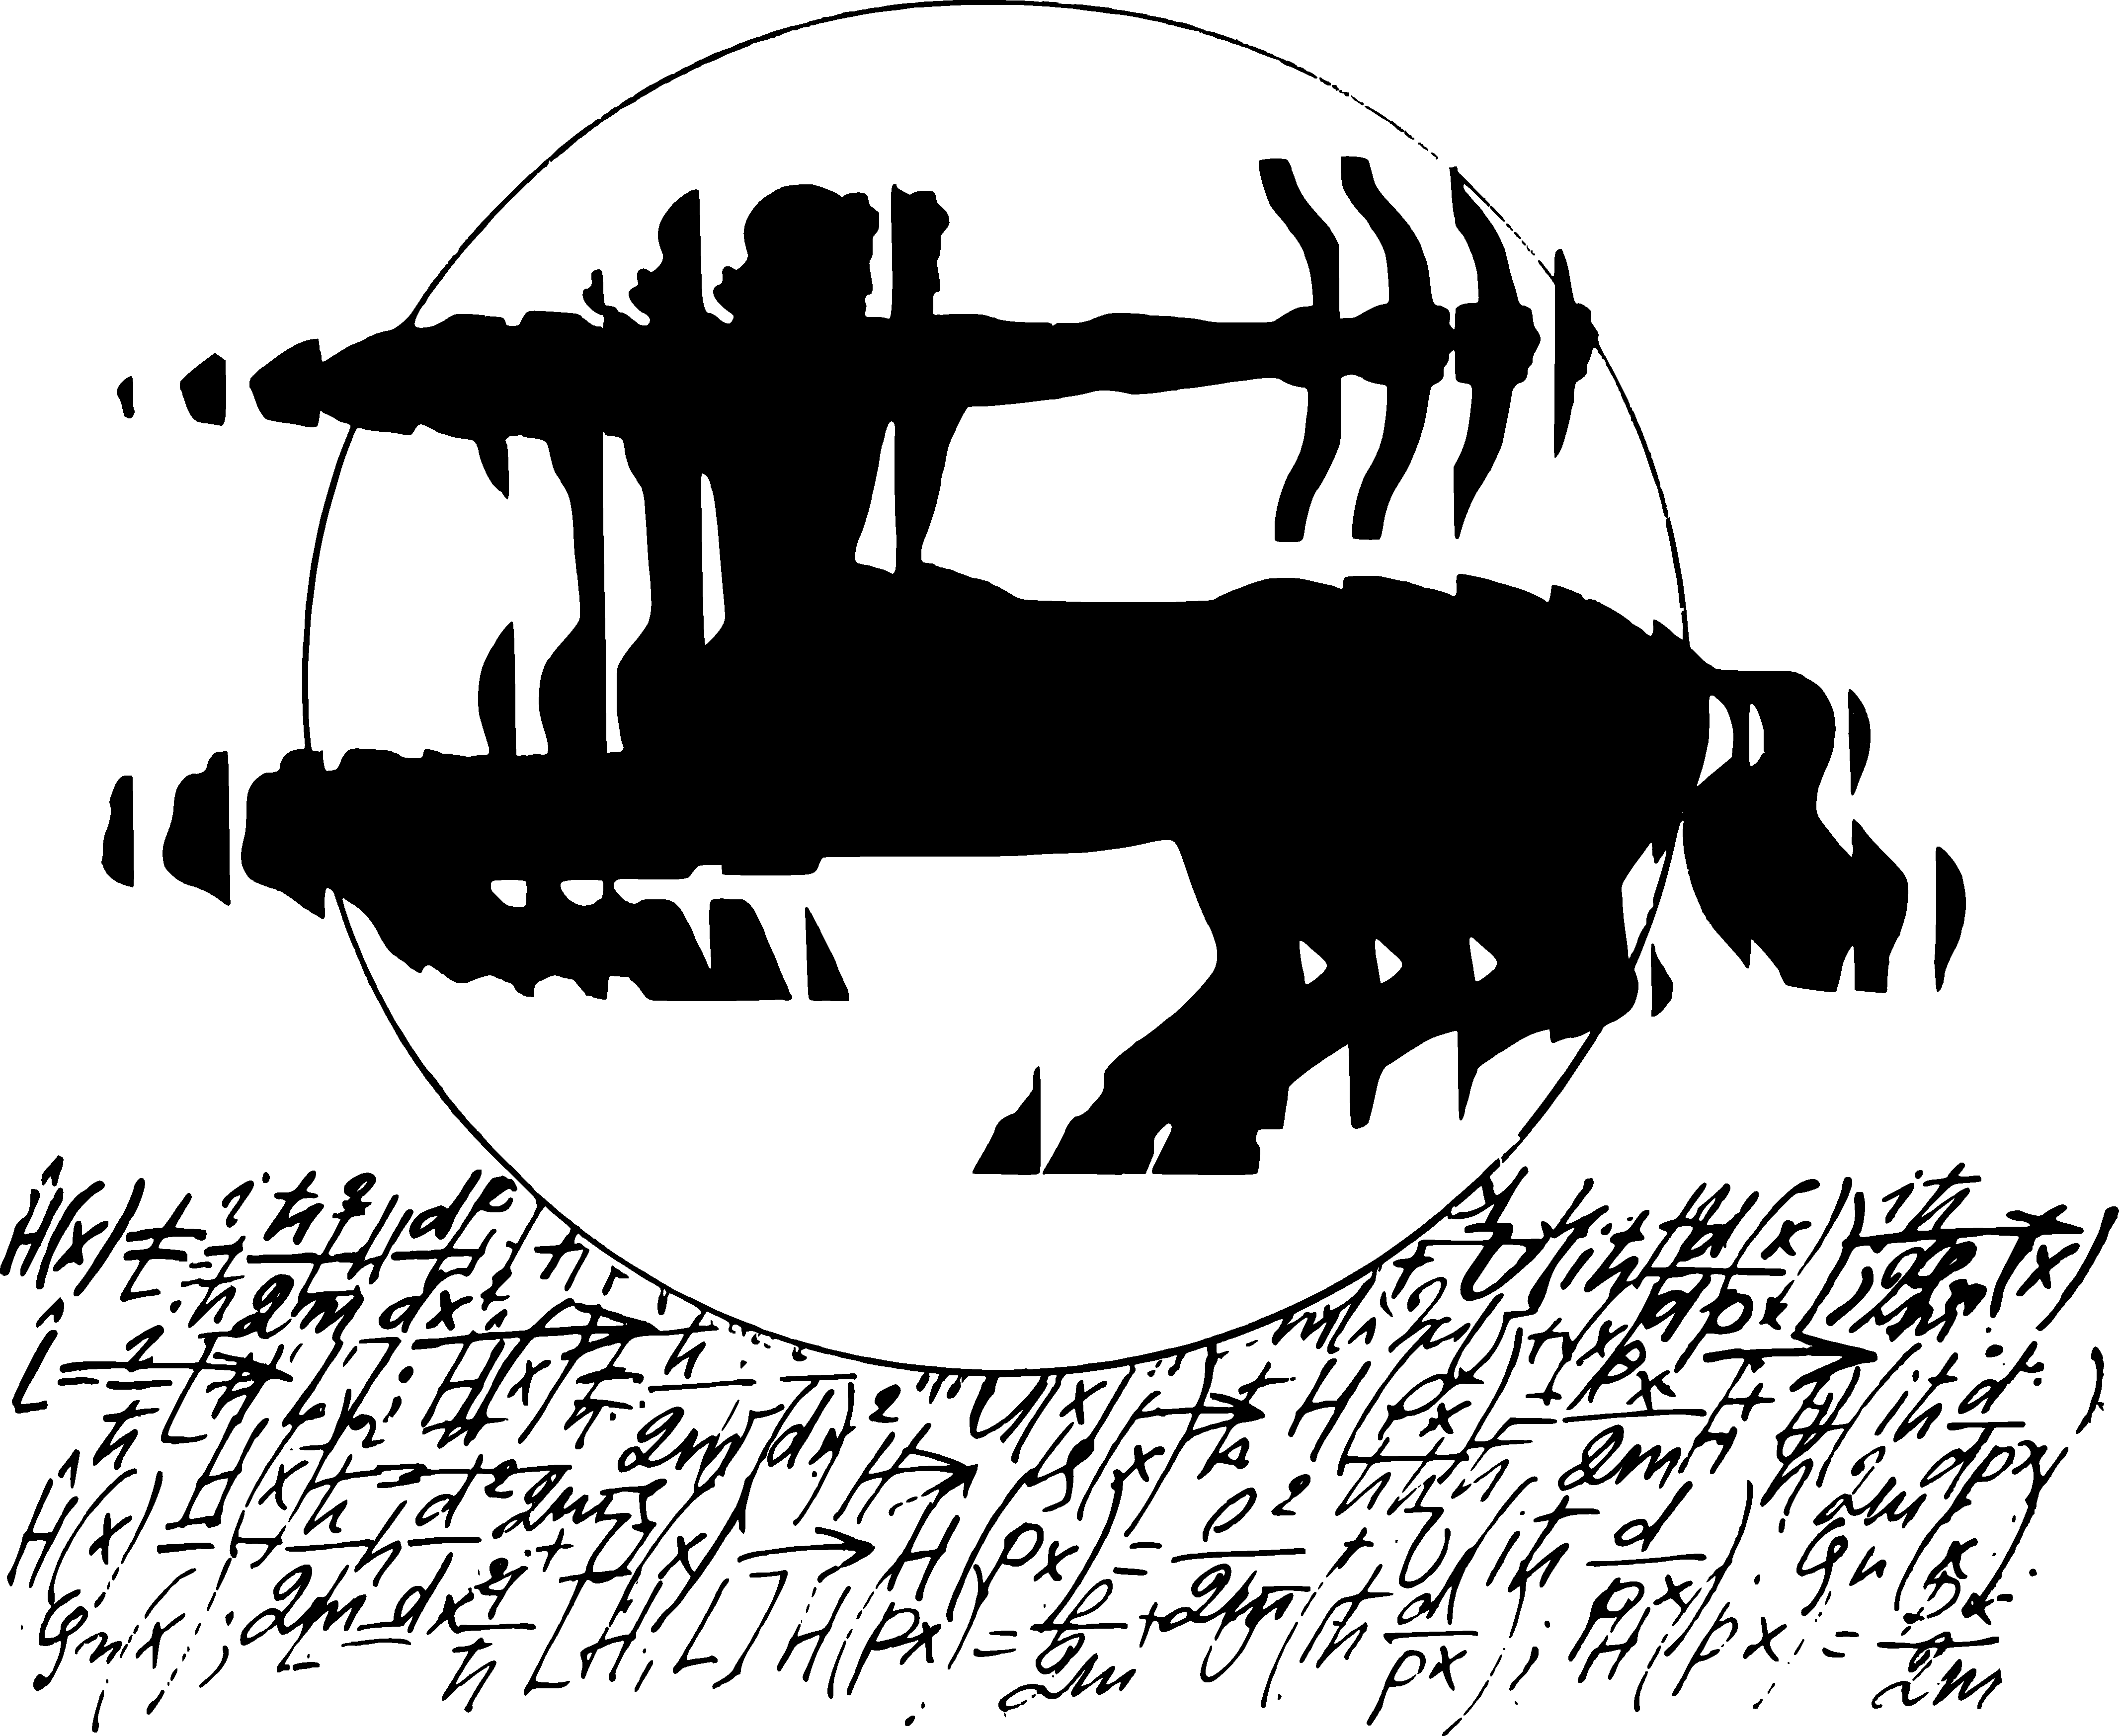
\includegraphics[width=\linewidth]{figures/ch-03.pdf}
%\label{}
\end{figure*}
\cleardoublepage

Every \marginnote{Some General Remarks}physical theory is a synthesis
of certain physical ideas (advanced on the basis of experiment) and a
certain mathematical apparatus. The building-up of a theory is a
complicated and controversial process developing according to
successive approximations. However, in this controversial process,
at least in its initial stage, a completely definite logical structure
is envisaged, including three logically successive stages: 
\begin{enumerate}[leftmargin=1cm, label=(\arabic*)]
\item a stage in which the basic ideas are formulated and interpreted,
  and the physical foundation of the theory is built;
\item a stage in which an adequate mathematical aparatus for the
  physical ideas is found and the physical ideas and the mathematical
  apparatus are linked together, i.e. it is postulated exactly what
  physical meaning corresponds to the various mathematical symbols (as
  a result, the mathematical relations acquire the meaning of physical
  laws), and
\item a stage in which the ``physicized'' mathematical apparatus is
  ``set to work'' The new results thus obtained are checked
  experimentally where this is possible. This leads to a further
  understanding of the physical content of theory and to a further
  development of its apparatus.
\end{enumerate}

At the time of creation of a theory the mathematical apparatus
adequate for the description of physical ideas mayor may not be
available. When Newton created his mechanics, he also had to work out
the corresponding mathematical apparatus -- the method of fluxions
which later developed into differential and integral calculus. But
when quantum mechanics was created, the appropriate mathematical
apparatus was already available in the form of \emph{theory of linear
  operators}.

In Quantum Physics and Philosophy\cite{bohr-1963}, Bohr writes \emph{
  \ldots in quantal formalism, the quantities by which the state of
  a physical system is ordinarily defined are replaced by symbolic
  operators subjected to a non-commutative algorism involving Planck's
  constant. This procedure'precents a fixation of such quantities to
  the extent which would be required tor the deterministic description
  of classical physics, but allows us to determine their spectral
  distribution as revealed by evidence about atomic processes. In
  conformity with the non-pictorial character of the formalism, its
  physical interpretation finds expression in laws, of an
  essentially statistical type \ldots}  

Turning to the mathematical aspect of quantum theory, we shall
consider below how quantum-mechanical ideas ``are introduced into'' the
apparatus of linear operators. We shall demonstrate the working of
this apparatus by a number of specially selected examples and
problems.  


\section{A Brief Look at the Theory of Linear Operators}
\label{sec-17}
This section is essentially mathematical in nature. It includes
different questions on the theory of linear operators. In other
words, it describes the fundamentals of the mathematical apparatus
which proved to he suitable for the creation of quantum theory. We
emphasize that in this section none of the mathematical symbols is
``loaded'' with any physical meaning.

An \marginnote{Linear Operators (Basic Definitions)}operator, when
applied to some function, transforms it into a new function. The
notation 
\begin{equation}%
\hat{L} \, \psi (x) = \varphi (x)
\label{eq-17.1} 
\end{equation}

means that the operator denoted the symbol  $\hat{L}$ acts on the function $\psi
(x)$, as a result of which we get function $\varphi (x)$. 

The operator $\hat{L}$ is called \emph{linear} if it satisfies the conditions:
\begin{equation}%
\begin{split}
\hat{L} \, (\psi_{1} + \psi_{2} ) & = \hat{L} \, \psi_{1} + \hat{L}
\, \psi_{2}\\
\hat{L}(a \psi) & = a \hat{L} \psi
\end{split}
\label{eq-17.2} 
\end{equation}
where $a$ is some number. We shall be using only linear operators
below. The effect of an operator acting on a function may be
represented as a definite or an improper integral:
\begin{equation}%
\hat{L} \, \psi (x) = \int L (x, y) \, \psi (y) dy
\label{eq-17.3} 
\end{equation}

The quantity $L (x, y)$ is called the \emph{kernel of the operator}.
If the variable is discrete, we will have instead of (\ref{eq-17.3})
\begin{equation}%
\hat{L} \, \psi_{n} = \sum_{m} L_{nm} \, \psi_{m} 
\label{eq-17.4} 
\end{equation}
The totality of coefficients $L_{nm}$ forms the \emph{matrix of the
  operator} $\hat{L}$, and we speak of the matrix representation of
the operator. A matrix representation is always possible because the
kernel $L (x, y)$ in (\ref{eq-17.3}) may obviously be treated as a
continuous matrix.

Suppose $\hat{L} \, \psi  = \varphi$; the operator $\hat{L}^{*}$ is called the \emph{complex
conjugate} of the operator $\hat{L}$, if by the action of this operator on
the function $\psi^{*}$ we get the function $\varphi^{*}$:
\begin{equation}%
\hat{L}^{*} \, \psi_{n}^{*} (x) = \varphi^{*}(x)
\label{eq-17.5} 
\end{equation}

The operator $\widetilde{\hat{L}}$ is said to be the \emph{transpose} of the operator
$\hat{L}$ if the following condition is satisfied:
\begin{equation}%
  \int \Psi (x) \, \hat{L} \, \psi (x) \, dx = \int \psi (x) \,
  \widetilde{\hat{L}} \, \Psi (x) dx
\label{eq-17.6} 
\end{equation}

The kernel of the transposed operator satisfies the condi- tion 
\begin{equation}%
\tilde{L} (x,y) = L(x,y)
\label{eq-17.7} 
\end{equation}

while the matrix satisfies the condition 
\begin{equation}%
\tilde{L}_{nm} = L_{nm}
\label{eq-17.8} 
\end{equation}

Let us consider some linear operator $\hat{L}$. Let us find its
complex conjugate operator $\hat{L}^{*}$. We then find the transposed
operator $\widetilde{\hat{L}}^{*}$ for the operator
$\hat{L}^{*}$. This operator is denoted by
$\hat{L}^{\dagger}$\sidenote{In the original typesetting symbol + is
  used to denote the conjujate, here we will be using $\dagger$ symbol.} and is
said to be conjugate to the operator  $\hat{L}$.  By using the concept of the
conjugate operator, two important types of linear operators are
defined: Hermitian operators and unitary operators. If
\begin{equation}%
\hat{L} = \hat{L}^{\dagger}
\label{eq-17.9} 
\end{equation}
the operator $\hat{L}$ is called \emph{Hermitian} (\emph{self-adjoint}). If 
\begin{equation}%
\hat{L} \, \hat{L}^{\dagger} = \hat{L}^{\dagger} \, \hat{L} =1 
\label{eq-17.10} 
\end{equation}

the operator $\hat{L}$ is said to be a \emph{unitary} operator. Note that
unitary operators are usually denoted by the symbol $\hat{U}$. The
matrix of a unitary operator satisfies the condition
\begin{equation}%
\sum_{m} U_{nm} U^{\dagger}_{mk} = \delta_{nk}
\label{eq-17.11} 
\end{equation}
Note an important property of unitary operators. Suppose 
\begin{equation*}
\sum_{m} U_{nm} \, \psi_{m} = \delta_{nk}
\end{equation*}
It can be easily seen that 
\begin{equation}%
\sum_{n} \varphi_{n}^{*} \, \varphi_{n} = \sum_{m} \psi_{m}^{*} \, \psi_{m}
\label{eq-17.12} 
\end{equation}
The basic equation of the theory of Iineas operators has the form
\begin{equation}%
\hat{L} \, \psi = \lambda  \psi
\label{eq-17.13} 
\end{equation}

The numbers $\lambda$ for which the equation (\ref{eq-17.13}) has
finite solutions, form the spectrum of \emph{eigenvalues} of the
operator $\hat{L}$. The spectrum of eigenvalues of an operator may be
continuous, discrete or mixed. The solutions $\psi (x)$ of equation
(\ref{eq-17.13}) are called the \emph{eigenfunctions} of the operator
$\hat{L}$. One or more \emph{eigenfunctions} may correspond to a given
eigenvalue. If $s$ linearly independent eigenfunctions correspond to a
certain value $\lambda_{1}$ it is said that the eigenvalue
$\lambda_{1}$ is $s$-fold degenerate.

We shall state three theorems concerning the basic Properties of
Hermitian Operators properties of Hermitian operators. (The proofs of
the first two theorems are given in \hyperref[appendix-a]{Appendix A}.)
\begin{description}[style=nextline, leftmargin=1cm, font=\rmfamily\bfseries]
\item[First Theorem]

An operator has real eigenvalues if and only if it is Hermitian.  

\item[Second Theorem]

The eigenfunctions of a Hermitian operator, corresponding to different
eigenvalues, are mutually orthogonal.  

Let $\hat{L} \, \psi_{n} = \lambda_{n} \, \psi_{n}$. The theorem states that
for $\lambda_{n} \ne \lambda_{m}$,
\begin{equation}%
\int \psi_{m}^{*} \,(x) \, \psi_{n} (x) dx = 0 
\label{eq-17.14}
\end{equation}

Since (\ref{eq-17.13}) is homogeneous, the eigenfunctions are determined
  upto an arbitrary constant multiplier. We choose this multiplier so
  that the normalization condition is satisfied: 
\begin{equation}%
\int \psi_{m}^{*} \,(x) \, \psi_{n} (x) dx = 1
\label{eq-17.15}
\end{equation}

By combining (\ref{eq-17.14}) and (\ref{eq-17.15}), we get the
condition of orthonormalization of the eigenfunctions of a Hermitian
operator:
\begin{equation}%
\int \psi_{m}^{*} \,(x) \, \psi_{n} (x) dx = \delta_{nm}
\label{eq-17.16}
\end{equation}

If the spectrum of the operator is continuous, we get instead of
(\ref{eq-17.16})
\begin{equation}%
\int \psi_{m}^{*} \,(x) \, \psi_{n} (x) dx = \delta (\lambda \lambda')
\label{eq-17.17}
\end{equation}

Let us consider the case of the $s$-fold degeneracy of an
eigenvalue. The eigenfunctions corresponding to this eigenvalue are,
generally speaking, not orthonormalized. However, we can form $s$ linear
combinations of the given functions which satisfy the condition of
orthonormalization.

\item[Third Theorem]

  Any bounded function may be expanded in a series (integral) of
  eigenfunctions of a Hermitian operator. In other words, the system
  of eigenfunctions of a Hermitian operator is a closed (complete)
  one.

  Using the last theorem, we represent any particular function $\Phi (x)$
  in the form of a series of eigenfunctions 
\begin{equation*}%
\psi_{n} (x): \Phi = \sum_{n} c_{n} \psi_{n}
\end{equation*}
In  order to find $c_{n}$, we multiply this equation by
$\psi_{m}^{*}\, (x)$ and integrate with respect to $x$:
\begin{equation*}%
\int \psi_{n}^{*} (x) \Phi \, (x) dx = \sum_{n} c_{n} \int \psi_{m}^{*} \,(x) \, \psi_{n} (x) dx
\end{equation*}
Using (\ref{eq-17.16}), we get from this
\begin{equation*}%
\int \psi_{n}^{*} (x) \Phi \, (x) dx = \sum_{n} c_{n} \delta_{mn} = c_{m}
\end{equation*}
Thus,
\begin{equation}%
\left.
\begin{split}
\Phi \, (x) & = \sum_{n } c_{n} \, \psi_{n} (x) \\
\textrm{where} & \\
c_{n} & = \int \psi_{n}^{*} (x) \, \Phi(x) \, dx
\end{split}
\; \right\}
\label{eq-17.18}
\end{equation}
In the case of a continuous spectrum, we must use the condition
(\ref{eq-17.17}). As a result, we get instead of (\ref{eq-17.18})
\begin{equation}%
\left.
\begin{split}
\Phi \, (x) & = \int c \, (\lambda) \, \psi_{\lambda} (x) \, d \lambda\\
\textrm{where} & \\
c (\lambda) & = \int \psi_{\lambda}^{*} (x) \Phi(x) \, dx
\end{split}
\; \right\}
\label{eq-17.19}
\end{equation}
We shall mention one of the results which is a direct consequence of
the completeness of the system of eigenfunctions of a Hermitian
operator. Suppose 

\begin{equation*}
\Phi(x) = \int c (\lambda) \, \psi_{\lambda} (x) \, d \lambda
\end{equation*}
and 
\begin{equation*}
\Psi(x) = \int b (\lambda') \, \psi_{\lambda'} (x) \, d \lambda'
\end{equation*}
By using (\ref{eq-17.17}), it can be easily seen that 
\begin{equation}%
\int \Psi^{*} (x) \, \Phi (x) \, dx = \int b^{*} (\lambda) \,
c(\lambda) \, d \lambda
\label{eq-17.20}
\end{equation}
\end{description}


Suppose \marginnote{Representations} that the Hermitian operator $M$
transforms the function $\Phi (x)$ into the function $\Psi (x)$ :

\begin{equation}%
\Psi (x) = \hat{M} \, \Phi (x) 
\label{eq-17.21}
\end{equation}
Let us expand the functions $\Phi$ and $\Psi$ in terms of
eigenfunctions $\psi_{\lambda} (x)$ of another Hermitian operator (the operator
$\hat{L}$). Assuming that the spectrum of the operator $\hat{L}$ is continuous, we
have 
\begin{equation}%
\begin{split}
\Phi(x) & = \int c (\lambda) \, \psi_{\lambda} (x) d \lambda \\
\Psi(x) & = \int b (\lambda) \, \psi_{\lambda} (x) d \lambda 
\end{split}
\label{eq-17.22}
\end{equation}

The transformation (\ref{eq-17.21}) will then have some corresponding
transformation of the function $c (\lambda)$ to the function $b (\lambda)$. We write
this transformation in the form 
\begin{equation}%
b (\lambda) = \hat{M} (\lambda) c (\lambda)
\label{eq-17.23}
\end{equation}

It is said that \ref{eq-17.21} and \ref{eq-17.23} are two different
representations of the same transformation. The nature of the
representation is determined by the variables on which the initial and
final functions depend. Hence we speak of $x$-representation in the case
of \ref{eq-17.21} and of $\lambda$-representation (representation of the
operator $\hat{L}$) in the case of \ref{eq-17.23}. Correspondingly, the
operator $\hat{M}$ in \ref{eq-17.21} is the operator of the given
transformation, defined in the $x$-representation [for convenience, we
shall henceforth write it as $\hat{M} (x)$], while the operator $\hat{M} (\lambda)$
occurring in \ref{eq-17.23} is the operator of the given
transformation, defined in $\lambda$-representation.

Let us see what the Hermitian operator looks like in eigen
representation. Let $\varphi_{\mu} (x)$ be the eigenfunctions of the
operator $\hat{M}$. In this case, we can write \ref{eq-17.22} in the
following form:
\begin{equation}%
\begin{split}
\Phi (x) & = \int c (\mu) \, \varphi_{\mu}(x) \, d \mu \\
\Psi (x) & = \int b (\mu) \, \varphi_{\mu}(x) \, d \mu 
\end{split}
\label{eq-17.24}
\end{equation}
Applying the operator if $\hat{M}(x)$ to the function $\Phi (x)$, we get
\begin{equation*}%
\begin{split}
\hat{M} (x) \Phi(x) & = \int c (\mu) \, \hat{M} \, \varphi_{\mu}(x) \,
d \mu \\
 & = \int \mu \, c (\mu) \, \varphi_{\mu}(x) \, d \mu 
\end{split}
\end{equation*}
Comparing this result with the second equality in \ref{eq-17.24}, we have 
\begin{equation}%
b (\mu) = \mu \, c (\mu)
\label{eq-17.25} 
\end{equation}
whence we get 
\begin{equation}%
\hat{M} (\mu) = \mu 
\label{eq-17.26} 
\end{equation}
Thus in its eigen representation, the Hermitian operator
coincides with its eigenvalues. 

We shall now consider a more general situation: the operator $\hat{M}(x)$
is known; it is required to find out the form of this operator in the
$\lambda$-representation. Using \ref{eq-17.21} and \ref{eq-17.22} we write
\begin{equation*}%
\begin{split}
\Psi(x) & =  \hat{M}(x) \, \Phi(x) \\
&= \int c(\lambda') \, \hat{M} (x) \, \psi_{\lambda} (x) \, d \lambda' \\
 & = \int c (\lambda') \, \psi_{\lambda'}(x) \, d \lambda' 
\end{split}
\end{equation*}
Multiplying both sides of the last of these equalities by $\psi^{*}_{\lambda} (x)$ and integrating with respect to $x$, we get 
\begin{equation*}%
\int c (\lambda') \left[ \int \psi^{*}_{\lambda} (x) \, \hat{M}(x) \,
  \psi_{\lambda'} (x) \, dx \right] d \lambda' = \int b(\lambda') \,
\left[ \int \psi^{*}_{\lambda} (x) \, \psi_{\lambda'}(x) \, dx \right]
d \lambda'
\end{equation*}

By using (\ref{eq-17.17}), we find that

\begin{equation*}%
b(\lambda) = \int \left[ \int \psi^{*}_{\lambda} (x) \, \hat{M}(x) \,
  \psi_{\lambda'} (x) \, dx \right] \, c (\lambda') \, d \lambda'
\end{equation*}

Lastly, by taking \ref{eq-17.23} into account, we finally get the result
[compare with \ref{eq-17.3}]:
\begin{equation*}%
\hat{M} (\lambda) \, c (\lambda) = \int M(\lambda, \lambda') \,
c(\lambda') \, d \lambda'
\end{equation*}
where 
\begin{equation}%
M(\lambda, \lambda') = \int  \psi^{*}_{\lambda} (x) \, \hat{M}(x) \,
  \psi_{\lambda'} (x) \, dx
\label{eq-17.27}
\end{equation}
Thus, if the form of the operator is known, say, in the
$x$-representation, we can find the matrix of this operator in the
$\lambda$-representation by using the eigenfunctions of, the operator
$\hat{L}$ given in the $x$-representation, by \ref{eq-17.27}.

In conclusion, we mention a situation where the eigenfunctions of
one Hermitian operator are given in the representation of another
operator. In this case, the following relation is valid: 
\begin{equation}%
  \psi_{\lambda'} (\mu) =  \phi^{*}_{\mu} (\lambda)
\label{eq-17.28}
\end{equation}

A \marginnote{Transition from One Representation to
  Another as Unitary Transformation}transition from the
$\lambda$-representation to the $x$-representation is determined with the help
of \ref{eq-17.22}. In operator form, these relations can be written as

\begin{equation}%
\begin{split}
\Phi (x) & = U(x, \lambda) \, c (\lambda) \\
\Psi (x) & =  U(x, \lambda) \, b (\lambda) 
\end{split}
\label{eq-17.29}
\end{equation}
Next, we put 
\begin{equation*}%
\begin{split}
\int \Psi^{*} (x) \, \Phi (x) \, dx & = \int \Psi^{*}(x) \, \hat{U}
(x, \lambda) \, c(\lambda) \, dx \\
& =  \int c(\lambda) \, \left[ \hat{U}^{\dagger} (\lambda, x) \Psi (x)
\right]^{*} \, d \lambda
\end{split}
\end{equation*}
Using \ref{eq-17.20}, we get
\begin{equation*}%
b(\lambda) =  \hat{U}^{\dagger} (\lambda, x) \, \Psi(x)
\end{equation*}
Two important results follow from the last formula. Firstly,
\begin{equation*}%
\begin{split}
\Psi(x) & =  \hat{U} (x, \lambda) \, b(\lambda) \\
& = \hat{U} (x, \lambda) \, \hat{U}^{\dagger} (\lambda, x) \, \Psi(x)
\end{split}
\end{equation*}
and, consequently, 
\begin{equation}%
\hat{U} (x, \lambda) \, \hat{U}^{\dagger} (\lambda, x) = 1
\label{eq-17.30}
\end{equation}
This means that the
transition from one representation to another is accomplished with the
help of a unitary transformation. Secondly, if 
$\Psi(x) =  \hat{M} (x) \, \Phi(x)$, then  
\begin{equation*}
\hat{U} (x, \lambda) \,
b(\lambda) = \hat{M}(x) \, \hat{U} (x, \lambda) \, c(\lambda) 
\end{equation*}
and, according to (\ref{eq-17.30}), 
\begin{equation}%
b(\lambda) =  \hat{U}^{\dagger} (\lambda, x) \, \hat{M}(x) \,
\hat{U} (x, \lambda) \, c(\lambda)
\label{eq-17.31} 
\end{equation}

Comparing \ref{eq-17.31} and \ref{eq-17.23}, we get
\begin{equation}%
\hat{M} (\lambda) = \hat{U}^{\dagger} (\lambda, x) \, \hat{M}(x) \,
\hat{U} (x, \lambda) 
\label{eq-17.32} 
\end{equation}
It should be explained here that a product of operators means the
successive action of the operators on the functions to their right. In
the present case we should first apply the operator $U (x, \lambda)$
to the function $c (\lambda)$, thus getting the function
$\Phi(x)$. Operator $\hat{M} (x)$ then acts on the function $\Phi(x)$,
resulting in the function $\Psi(x)$. Finally, the function $\Psi (x)$ is
acted on by the operator  $\hat{U}^{\dagger} (\lambda, x)$.


Thus, the relations \ref{eq-17.29} describe the transition from one
representation of functions to another carried out with the help of a
unitary operator. Relation \ref{eq-17.32} describes the same
transition for operators.

Quantities \marginnote{Unitary Invariants}and properties which do not
change with unitary transformations and are, consequently, independent
of the choice of representation are called \emph{unitary inuariants}. Unitary
invariants include: 
\begin{enumerate}[label=(\alph*), leftmargin=1cm]
\item the Hermitian property of an operator (if an operator is
  Hermitian in one representation, it will he Hermitian in any other
  representation);
\item the spectrum of eigenvalues of a Hermitian operator;
\item the condition of orthonormalization of eigenfunctions [this is
  immediately seen from \ref{eq-17.12}];
\item integrals of the type $\int \Psi^{*} (x) \, \Phi (x) \, dx $ [this directly
  follows from \ref{eq-17.20}];
\item integrals of the type $\int \Psi^{*} \, \hat{M} (x) \, \Phi(x)
  \, dx$ and of the more general type $\int \Psi^{*} \, \hat{M}^{n} (x) \, \Phi(x)
  \, dx $, where $n$ is a positive integer.
\end{enumerate}

Note that unitary invariance of these integrals means that the
following relations hold:

\begin{align}%
\int \Psi^{*} \, \hat{M}(x) \, \Phi(x) \, dx & = \int b^{*}(\lambda) \,
\hat{M} (\lambda) \, c (\lambda) \, d \lambda   
\label{eq-17.33} \\
\int \Psi^{*} \, \hat{M}^{n}(x) \, \Phi(x) \, dx & = \int b^{*}(\lambda) \,
\hat{M}^{n} (\lambda) \, c (\lambda) \, d \lambda 
\label{eq-17.34} 
\end{align}

As an example we shall prove \ref{eq-17.33}. Using \ref{eq-17.29} and
\ref{eq-17.32}, we successively transform the left-hand side of
(17.33): 
\begin{equation*}
\begin{split}
\int \left[ \hat{U}^{*}\, b^{*}(\lambda)  \right] \hat{U} \, \hat{M}
(\lambda) \, \hat{U}^{\dagger} \, \hat{U} \, c(\lambda) \, dx & = 
\int \left[ \hat{U}^{*}\, b^{*}(\lambda)  \right] \hat{U} \, \hat{M}
(\lambda) \, c(\lambda) \, dx\\
& = \int b^{*}(\lambda) \, \hat{U}^{\dagger} \, \hat{U} \, \hat{M}
(\lambda) \, c (\lambda) \, d \lambda \\
& = \int b^{*}(\lambda) \, \hat{M}(\lambda) \, c(\lambda) \, d \lambda
\end{split}
\end{equation*}
Thus, as a result, we get the right-hand side of \ref{eq-17.33}, Q.E.D.  

Two \marginnote{Commutation of Operators and the System of Common
  Eigenfunctions} operators $\hat{L}$ and $\hat{M}$ are called
\emph{commutative} if for any bounded function $\Phi(x)$ satisfy the
following condition:
\begin{equation}%
\hat{M} \, \hat{L} \, \Phi (x) = \hat{L} \, \hat{M} \, \Phi (x)
\label{eq-17.35} 
\end{equation}
If there is even one function for which \ref{eq-17.35} does not hold,
the operators $\hat{L}$ and $\hat{M}$ are called non-commutative. The
notation 
\begin{equation*}%
[\hat{M}, \, \hat{L}] = \hat{M} \, \hat{L} - \hat{L} \, \hat{M} 
\end{equation*}
is called the \emph{commutator operator} of $\hat{L}$ and
$\hat{M}$. If the operators commute, this fact is often expressed
thus:
\begin{equation*}%
[\hat{M}, \, \hat{L}] = 0
\end{equation*}
The following \emph{theorem} holds: If the operators $\hat{L}$ and
$\hat{M}$ have common eigenfunctions forming a closed system, the
operators commute. We shall prove this theorem.

We denote the eigenfunctions of the operators $\hat{L}$ and $\hat{M}$
by $\psi_{\lambda \mu} (x)$. (The double subscript $\lambda \mu$
indicates the fact that these functions are common). Obviously,
\begin{equation*}%
\begin{split}
\hat{M}\,\hat{L} \, \psi_{\lambda \mu} & = \lambda \, \hat{M}
\,\psi_{\lambda \mu} \\
& = \lambda \, \mu \, \psi_{\lambda \mu} \\
\hat{L}\,\hat{M} \, \psi_{\lambda \mu} & = \mu \, \hat{L} \,
\psi_{\lambda \mu} \\
& =  \mu \,  \lambda \, \psi_{\lambda \mu} \\
\end{split}
\end{equation*}
It follows from this that 
\begin{equation*}%
  (\hat{M}\,\hat{L} - \hat{L} \, \hat{M}) \, \psi_{\lambda \mu} =0
\end{equation*}
and since the functions $\psi_{\lambda \mu} (x)$ are known to form a closed system, for any function $\Phi (x)$ we can write
\begin{equation*}%
\begin{split}
  (\hat{M}\,\hat{L} - \hat{L} \, \hat{M}) \, \Phi(x) & = \sum
  c_{\lambda \mu} \, (\hat{M}\,\hat{L} - \hat{L} \, \hat{M}) \,
  \psi_{\lambda \mu }(x) \\
& = 0
\end{split}
\end{equation*}

Q.E.D. 

We stress the importance of the fact that common eigenfunctions must
form a closed system. It may so happen that two operators have only
one common eigenfunction. In this case it is impossible to draw any
conclusion about the commutativity of the operators.

The above theorem means that commutativity of operators is a necessary
property of the commonness of the system of eigenfunctions of these
operators. But is this property a sufficient condition also?  The
answer to this question is in the affirmative in the case when there
is no degeneracy in the eigenvalues of the operators. In the more
general case, taking into account the possibility of degeneracy, the
following \emph{theorem} is valid. If the operators $\hat{L}$ and
$\hat{M}$ commute, we can find their common eigenfunctions. For
example, suppose the eigenvalue $\lambda_{1}$ is $s$-fold
degenerate. From the $s$ solutions of the equation $\hat{L} \, \psi =
\lambda_{1} \, \psi$, we can choose $s$ linear combinations which are
also the eigenfunctions of the operator $\hat{M}$. In this case,
$\lambda_{1}$ will in general correspond to $s$ different eigenvalues
of the operator $\hat{M}$.

With this we conclude our degression in the field of ``pure''
mathematics. The information contained here is sufficient for further
use of the apparatus of linear operators without referring to special
literature.  
\section{From Hamiltonian Matrix to Energy Operator}
\label{sec-18}

We \marginnote{The Influence of the Choice of Basic States}turn to
equation \ref{eq-12.8} discussed in Section \ref{sec-12}. There we
chose a certain system of basic states of microparticle $ \left\{
    \bra{i} \right\}$. An arbitrary state $\bra{s(t)}$ of this
microparticle at time $t$ was represented as a superposition of these
basic states:
\begin{equation}%
\Bra{s(t)} = \sum_{i} \Braket{s(t)| i} \bra{i}
\label{eq-18.1}
\end{equation}

The notation $C_{i} (t)$ was employed for the amplitudes $\Braket{s
  (t)| i}$. It was shown that the amplitudes $C_{i} (t)$ satisfy the
equation
\begin{equation}%
- i \hbar \frac{d}{dt} C_{i}(t) = \sum H_{ij} (t) C_{j}(t)
\label{eq-18.2}
\end{equation}
which permits one to find, from a knowledge of the amplitudes $C_{i} (t)$ and the Hamiltonian matrix $H_{ij} (t)$ at time $t$, the amplitudes $C_{i}$ at any subsequent moments of time.

The expression \ref{eq-18.1} clearly shows that the set of amplitudes
$\left \{ C_{i} (t) \right \}$ depends on the choice of the system of
basic states $ \left \{ \bra{i} \right \} $. Suppose we have to go over
to a new system of basic states $ \left \{ \bra{m} \right\}$. In
order to accomplish this transition, we represent the earlier basic
states in the form of superposition of new basic states: 
\begin{equation}%
\bra{i} = \sum_{m} \braket{i|m} \bra{m}
\label{eq-18.3}
\end{equation}
Substituting this superposition in \ref{eq-18.1}, we get 
\begin{equation*}%
\bra{s(t)} = \sum_{i} \sum_{m} C_{i} (t) \, \braket{i|m} \bra{m}
\end{equation*}
or 
\begin{equation}%
\bra{s(t)}  = c_{m}(t) \, \bra{m}
\label{eq-18.4}
\end{equation}
where
\begin{equation}%
c_{m}(t) = \sum_{i} C_{i}(t) \, \braket{i|m}
\label{eq-18.5}
\end{equation}
The new amplitudes $c_{m} (t)$, corresponding to the system of  $ \left\{ \bra{m} \right\}$, satisfy an equation of the type \ref{eq-18.2} but obviously with a new
Hamiltonian matrix $H_{mn} (t)$:
\begin{equation}%
- i \hbar \, \frac{d}{dt} \, c_{m}(t) = \sum_{n} H_{mn} (t) \, C_{n}(t)
\label{eq-18.6}
\end{equation}
We shall show how the old Hamiltonian matrix can he expressed in terms
of the new one. Substituting \ref{eq-18.5} in \ref{eq-18.6}, we find
\begin{equation*}%
- i \hbar \, \frac{d}{dt} \, \sum_{j'} C_{j'}(t) \braket{j'|m} =
\sum_{n} \sum_{j} H_{mn} (t) \, C_{j}(t) \braket{j|n}
\end{equation*}
Multiplying both sides of the last equation by $\braket{m|i}$ and summing with
respect to $m$, we get
\begin{equation*}%
\begin{split}
 - i \hbar \, \frac{d}{dt} & \, \sum_{j'} C_{j'}(t) \left[
 \sum_{m} \braket{j'|m} \, \braket{m|i} \right] \\
 & = \sum_{j} \left[ \sum_{n} \sum_{m} H_{mn} (t) \,
   \braket{j|n} \, \braket{m|i} \right] \, C_{j} (t)
\end{split}
\end{equation*}

Taking into account that 
\begin{equation*}%
\sum_{m} \braket{j'|m} \, \braket{m|i} = \braket{j'|i} = \delta_{j' i} 
\end{equation*}
we can simplify the left-hand side of the last equation. As a result, we get 
\begin{equation*}%
- i \hbar \, \frac{d}{dt} \, C_{i}(t)  = \sum_{j}  H_{ij} (t) \, C_{j}(t)
\end{equation*}
where
\begin{equation}%
H_{ij}(t) = \sum_{n} \sum_{m} H_{mn} (t) \, \braket{j|n} \, \braket{m|i}
\label{eq-18.7}
\end{equation}
Thus the choice of any system of basic states of a microparticle
influences both the form of the amplitudes of states satisfying \ref{eq-12.8}
as well as the form of the Hamiltonian matrix.

It was mentioned in Section \ref{sec-13} that the system of basic
states is usually chosen in such a way that these states could have a
direct physical meaning. However, for the sake of greater convenience
when considering equation \ref{eq-12.8}, we go over to new, specially
selected basic states in a number of cases. Thus, in Section
\ref{sec-13}, the transition from the basic states $\bra{1}$ and
$\bra{2}$ to the basic states $\bra{\mathrm{I}}$ and $\bra{\mathrm{II}}$ was motivated
by a desire to diagonalize the Hamiltonian matrix, while in Section
\ref{sec-14} it was done in order to express the Hamiltonian matrix in
a form convenient for drawing an analogy with an electron in magnetic
field.

Let \marginnote{Transformation of an Equation Expressing Causality
  Into a Form Independent of the Choice of Basic States}us consider
operator $\hat{H} (t)$ satisfying the following relation:
\begin{equation}
H_{ij} (t)=  \braket{j | \hat{H} (t)| i}
\label{eq-18.8}
\end{equation}
The operator $\hat{H} (t)$, acting on the basic state $\bra{i}$, gives
rise to a new state $\bra{\psi (t)} = \hat{H} (t) \bra{i}$, which is
not basic. The element of the Hamiltonian matrix $H_{ij} (t)$ here plays
the role of the amplitude $\braket{j|\psi (t)}$ , i.e. of the amplitude
probability that a microparticle in the basic state $\bra{j}$ may be found
in the state $\bra{\psi (t)}$. Substituting \ref{eq-18.8} in \ref{eq-18.2}, we get
\begin{equation}
- i \hbar \, \frac{d}{dt} \, \braket{s(t)| i} = \sum_{j}
\braket{s(t)| j} \braket{j| \hat{H} (t)|i}
\label{eq-18.9}
\end{equation}
or
\begin{equation}
- i \hbar \, \frac{d}{dt} \, \braket{s(t)| i} = \braket{s(t)| \hat{H} (t)|i}
\label{eq-18.10}
\end{equation}

Taking the complex-conjugate of the equation and considering \ref{eq-9.33} and \ref{eq-12.9}, we get 
\begin{equation}
- i \hbar \, \frac{d}{dt} \, \braket{i |s(t)} = \braket{i| \hat{H} (t)|s(t)}
\label{eq-18.11}
\end{equation}
or 
\begin{equation}
- i \hbar \, \frac{d}{dt} \, \bra{s(t)} = \hat{H} (t) \Braket{s(t)}
\label{eq-18.12}
\end{equation}
Note that while going over from \ref{eq-18.9} to \ref{eq-18.10} or
from \ref{eq-18.11} to \ref{eq-18.12}, we have made use of the rules
given in Section \ref{sec-10} under the heading ``The Mechanics of Quantum
Mechanics''. The final equation \ref{eq-18.12} is analogous to equation
\ref{eq-18.2}, but unlike the latter, it is independent of the choice of
basic states.

In \marginnote{Vector Analogy} order to express the causal
relationship mathematically \ref{eq-18.2} in the above discussion, we
had to use information about the state under consideration, the
physical meaning of the problem and the system of basic states. But
now [Eq. \ref{eq-18.12}] it is sufficient to have information about the state
under consideration and the physical meaning of the problem. This
means that a transition from \ref{eq-18.2} to \ref{eq-18.12} leads to a more
abstract level of analysis.

We emphasize that such an abstraction is made possible by the use of
operators. Operators help us to get quantum-mechanical relations that
are more abstract and are \emph{independent} of the choice of the system of
basic states.

The more abstract analysis, enabled by the introduction of operators
is, to a certain extent, analogous to the more abstract analysis
connected with the introduction of vectors. We shall consider this
analogy in detail. 

This analogy is not unexpected. Remember that in Sec. \ref{sec-14} it was
suggested that a state should be treated as a vector in some arbitrary
space. The concept of projection amplitudes was also introduced
there.

The essence of the \emph{vector analogy} is as follows. In order to
perform operations with components of vectorial quantities one always
has to choose a definite system of coordinate axes. In quantum
mechanics we make a corresponding choice of a definite system of basic
states. By using vectors, one can perform operations with vector
quantities without resorting to a choice of any particular system of
axes. Similarly, by using vectors of states and their operators in
quantum mechanics, one can avoid having to choose a system of basic
states. Let us illustrate the vector analogy with the help of the
Table \ref{vector-analogy-table}.

\begin{table}
\begin{tabular}{ll}
\toprule
\textbf{Quantum-mechanical expression} & \textbf{Vector Analogy}\\[8pt]
%\hline
\midrule
\vspace*{5pt}
$\displaystyle\sum_{i} \braket{f|i}\braket{i|s} = 0$ & $\displaystyle\sum_{i} a_{i}b_{i} =0$ \\ [5pt] 
$\braket{f|s} =0 $ & $\vec{a} \, 
\vec{b} = 0$\\
(Mutually orthogonal states) &  (Mutually orthogonal vectors) \\[3pt]
\midrule
%\hline 
$i \hbar \, \dfrac{d}{dt} \, \braket{i|s(t)} = \displaystyle\sum_{j} H_{ji}
\, \braket{j|s(t)}$ & $c_{i} = \displaystyle\sum_{j} H_{ij} \, a_{j}$ \\[8pt]
$i \hbar \, \dfrac{d}{dt} \bra{s(t)} = \hat{H} \bra{s(t)}$ & $\vec{c}
= \hat{H} \, \vec{a}$\\[3pt]
(Operation on a state) & (Operation on a vector)\\
\bottomrule
\end{tabular}
\label{vector-analogy-table}
\end{table}

Each cell of the table contains two expressions having the same
meaning (indicated in brackets). However, the upper expression depends
on the choice of the system of basic states or coordinate axes, while
the lower one is independent of any such choice.


It is worthwhile giving an example for the lower right cell of the
above table, which shows how one can imagine an operator acting on a
vector. As an example of this (to which, of course, no
``quantum-mechanical meaning'' should be assigned) let us consider the
case when the matrix $H_{ij}$ is of the form 
\begin{equation*}
\begin{pmatrix}
H
\end{pmatrix}
=
\begin{pmatrix}
0 & -\dfrac{\partial}{\partial r_{3}} &  \dfrac{\partial}{\partial
  r_{2}}\\
\dfrac{\partial}{\partial r_{3}} & 0 & -\dfrac{\partial}{\partial r_{1}}
\\
-\dfrac{\partial}{\partial r_{2}} & \dfrac{\partial}{\partial r_{1}} &
0 
\end{pmatrix}
\end{equation*}
where $r_{1}, \, r_{2}, \, r_{3}$ are three Cartesian coordinates in
space. In this case the relation $\vec{c} = \hat{H} \vec{a}$ acquires
the form which is familiar to those who have studied vector analysis:
$\vec{c} = \vec{\nabla} \times \vec{a}$.

In conclusion let us reiterate the various aspects of the vector
analogy: 
\begin{enumerate}[label=(\alph*), leftmargin=1cm]
\item corresponding to the choice of basic states, we have a choice of
  the system of coordinate axes;
\item a transition from one set of basic states to another corresponds
  to a transition from one system of axes to another (note that such a
  transition does not involve the physics of the problem being
  considered);
\item the expansion into basic states corresponds to a representation
  of the vector in terms of its projections on the coordinate
  axes. The analogy with vectors is a good example of abstraction and
  of the representation of relations in a form taking into account
  only strictly physical information.
\end{enumerate}

Let \marginnote{Average Energy}us demonstrate some of the advantages
of the operator approach. We shall show how the mean value $\braket{E}$ of
the energy of a microparticle in some state $\bra{s}$ is determined. Let
$\left\{\bra{i}\right\}$ be the basic states with energies $E_{i}$. This means (see
Section \ref{sec-13}) that the Hamiltonian matrix is diagonal. Hence,
\begin{equation*}%
\braket{j| \hat{H}| i} = \delta_{ij} \, E_{i}
\end{equation*}
or 
\begin{equation}%
\braket{j| \hat{H}| i} = \braket{j|i} \, E_{i}
\label{eq-18.13} 
\end{equation}
We expand the state $\bra{s}$ in terms of the system of basic states
\begin{equation*}%
\left\{\bra{i} \right\} \, \bra{s} = \sum_{i} \braket{s|i} \bra{i}
\end{equation*}
and try to find the mean value of the energy $\braket{E}$ with the help of a formula of the type \ref{eq-12.3}:
\begin{equation}%
\braket{E} = \sum_{i} |\braket{s|i}|^{2} \, E
\label{eq-18.14}
\end{equation}
By taking \ref{eq-9.33} into account, we rewrite \ref{eq-18.14} in the
form 
\begin{equation}%
\braket{E} = \sum_{i} \braket{s|i}^{2} E_{i} \, \braket{i|s} \equiv \braket{s|\varphi}
\label{eq-18.15}
\end{equation}
where 
\begin{equation}%
\bra{\varphi} = \sum_{i} \bra{i} E_{i} \, \braket{i|s}
\label{eq-18.16}
\end{equation}
From \ref{eq-18.13} it follows that 
\begin{equation}%
\hat{H} \bra{i} = \bra{i} E_{i}
\label{eq-18.17}
\end{equation}
Substituting \ref{eq-18.17} in \ref{eq-18.16}, we get
\begin{equation*}%
\bra{\varphi} = \sum_{i} \hat{H} \, \bra{i} \, \braket{i|s} = \hat{H} \bra{s}
%\label{eq-18.16}
\end{equation*}
after which we get the required result from \ref{eq-18.15}:
\begin{equation}%
\braket{E} = \braket{s|\hat{H}| s}
\label{eq-18.18}
\end{equation}
It can be seen from \ref{eq-18.18} that mean value of the energy of a
microparticle in the state $\bra{s}$ is expressed only through the operator
$\hat{H}$. Basic states do not enter this relation. 

The convenience of the relation \ref{eq-18.18} is due to its
independence from the choice of basic states, which allows one to use
freely any system of basic states when carrying out calculations. For
example, suppose it is convenient to use the basic states
$\left\{(\braket{m \, l}\right\}$. In this case the operator relation
\ref{eq-18.18} immediately acquire the corresponding form 
\begin{equation}%
\braket{E} = \sum_{m} \sum_{n} \braket{s|m} \braket{m|\hat{H}|n} \braket{n|s}
\label{eq-18.19}
\end{equation}

It has \marginnote{Energy Operator (Hamiltonian)}been mentioned above
that the Hamiltonian matrix could be called the energy matrix
(remember that the elements of the diagonalized Hamiltonian matrix are
essentially the possible values of the energy of the
microparticle). The connection between the operator $\hat{H}$ and the
Hamiltonian matrix as well as relation \ref{eq-18.18}, expressing the average
energy of a microparticle in terms of the operator $\hat{H}$, justify the name
\emph{energy operator} given to it. In the literature the operator it is also
called the \emph{Hamiltonian}.

We write expressions derived above in which the Hamiltonian of a
microparticle is present (we emphasize the exceptional importance of
these expressions): 
\begin{align}
i \hbar \, \frac{d}{dt} \bra{s(t)} = \hat{H} \, \bra{s(t)}
\label{eq-18.12} \\
\braket{E} = \braket{s|\hat{H}|s} 
\label{eq-18.18} \\
\hat{H} \, \bra{f} = \bra{f} \, E
\label{eq-18.20}
\end{align}

In expression \ref{eq-18.20}, $\bra{f}$ denotes some stationary state
and $E$ is the energy in this state.

Finally, we note that the Hamiltonian (as well as any other operator) may act not only on the state $\bra{s}$, but also on its amplitude $\braket{i|s}$, since we always have the representation [see \ref{eq-17.4}]
\begin{equation}%
\hat{H} \,C_{i} (t) = \sum_{j} H_{ij} \,C_{j} (t)
\label{eq-18.21}
\end{equation}

Using \ref{eq-18.21} and taking into account that $\braket{i| s}  =
C_{i}^{*}$, we can rewrite \ref{eq-18.2} in a form which, as can be
easily seen, is completely analogous in form to \ref{eq-18.12}:
\begin{equation}%
i \hbar \, \frac{d}{dt} \braket{i|s(t)} = \hat{H} \braket{i|s(t)}
\label{eq-18.22} 
\end{equation}
Correspondingly, \ref{eq-18.20} may he written in the form
\begin{equation}%
\hat{H} \braket{i|f} = E \braket{i|f}
\label{eq-18.23}
\end{equation}
\section{Linear Operators in Quantum Mechanics}
\label{sec-19}
We now come to the main problem of this chapter, i.e, that of imparting physical meaning to the mathematical apparatus of linear operators in order to convert it into the apparatus of quantum mechanics. In this sense the previous section should be considered as a preliminary step towards solving this problem.

The \marginnote{Role of Operators in Quantum Mechanics}following two
points must be noted when considering the role of linear operators
in quantum mechanics. 
\begin{description}[leftmargin=1cm]
\item[Firstly], in quantum mechanics to every dynamic variable (spatial
coordinate, energy, momentum, angular momentum, etc.), there is
assigned a definite Hermitian operator. 
\item[Secondly], the transition from one representation to an- other
  without changing the physical meaning of the prob- lem is achieved
  with the help of unitary operators.
\end{description}
Let us consider the first point in detail. It means that besides the
energy operator$\hat{H}$, other ``physical operators'' like the
coordinate operator $\vec{r}$ the momentum operator $\vec{p}$, the
angular momentum operator $\vec{M}$, etc. must be introduced. In
this respect, it is significant that the well-known dynamic relations
of classical mechanics may be transferred to quantum mechanics in the
same form, if we replace the physical quantities in these relations by
the corresponding Hermitian operators. In other words, the apparatus
of quantum mechanics may be built up in analogy with the apparatus of
classical mechanics, if we replace the dynamic variables with their
corresponding Hermitian operators. As an example, let us compare the
following expressions:

\begin{table}
\begin{tabular}{p{4cm}p{4cm}}
\toprule
\textbf{In classical mechanics} & \textbf{In Quantum Mechanics}\\[3pt]
%\hline
\midrule
\begin{minipage}{4cm}\begin{equation*} E = \frac{p^{2}}{2m} + U \end{equation*}\end{minipage} & \begin{minipage}{4cm}\begin{equation} \hat{H} = \frac{\hat{p}^{2}}{2m} + \hat{U} \label{eq-19.1}\end{equation}\end{minipage}\\
%\vspace*{3pt}
%\midrule
%\hline 
\begin{minipage}{4cm}\begin{equation*} \vec{M} = \left( \vec{r}
      \times \vec{p} \right) \end{equation*}\end{minipage} & \begin{minipage}{4cm}\begin{equation}  \vec{\hat{M}} = \left( \vec{\hat{r}}
      \times \vec{\hat{p}} \right)  \label{eq-19.2}\end{equation}\end{minipage}\\[5pt]
%\vspace*{3pt}
\bottomrule
\end{tabular}
\label{correspondence-table}
\end{table}

It should be remembered, however, that a complete formal analogy
between the apparatus of classical and quantum mechanics does not
exist. We point out (for details see Section \ref{sec-20}) that in the
algebraic manipulation of operator relations we must remember that
operators may not commute. Thus if $\hat{A}$ and $\hat{B}$ do not
commute, then $\left( \hat{A} + \hat{B} \right)^{2} \ne \hat{A}^{2} + 2 \hat{A}
\hat{B} + \hat{B}^{2}$. In this case $\left( \hat{A} + \hat{B} \right)^{2} =
\hat{A}^{2} +  \hat{A} \hat{B} + \hat{B}\hat{A} +\hat{B}^{2}$. Besides, there are
operators in quantum mechanics which do not have classical analogies
(for example, the spin operator).


Note that we may formally assign corresponding operators to all
classical dynamical variables including those which do not have any
meaning in the microworld.

Thus, we may introduce the operators of velocity $\hat{\vec{v}}$, of
potential energy $\hat{U}$, kinetic energy $\hat{T}$, etc., though
neither velocity nor the breaking-up of total energy into kinetic and
potential components which is characteristic for classical mechanics,
have any meaning for microparticles.

Let \marginnote{Basic Postulates}us consider the question: In exactly
what way can we compare a physical quantity with a Hermitian operator?
In other words, what is the meaning of the word ``compare'' here? The
following two basic postulates provide an answer to this question.

\begin{description}[leftmargin=1cm]
\item[Postulate 1.] If the operator $\hat{L}$ is compared with a physical
quantity $l$, it means that the eigenvalues $\lambda$ of the operator are
identified with the values of the physical quantity under
consideration obtained by measurement.
\item[Postulate 2.] If operator $\hat{L}$ is compared with a physical
  quantity $l$, it means that the eigenfunctions
  $\psi_{\lambda}(\alpha)$ of the operator are identified with the
  eigenfunctions of the quantities from the $\lambda$-set, expressed
  in $\alpha$-representation. By the remarks made in Section
  \ref{sec-15}, this means that the eigenfunctions  $\psi_{\lambda}(\alpha)$ of the
  operator are identified with the amplitudes of $\braket{\lambda | \alpha}$, often
  called the wave functions.
\end{description}

Thus a study of the fundamental equation of the theory of linear
operators [see \ref{eq-17.13}]
\begin{equation}%
\hat{L}(\alpha) \braket{\lambda|\alpha} = \lambda \braket{\lambda|\alpha}
\label{eq-19.3}
\end{equation}

includes physical problems such as finding the spectrum of possible
values $\lambda$ of a physical quantity $l$, and finding the
amplitudes of states $\braket{\lambda|\alpha}$ in which the
corresponding values of $\lambda$ occur. When applied to the energy
operator, \ref{eq-19.3} takes the form of \ref{eq-18.23}. A study of equation
\ref{eq-18.23} permits us to find the possible values of the energy of a
microparticle and the corresponding amplitude values of the stationary
states.


The \marginnote{Mathematical Results and Their Physical
  Meaning}postulates formulated above ``knit together'' the physical
and mathematical aspects; they ``load'' the mathematical symbols and
inferences with a definite physical meaning. We shall demonstrate this
with a number of observations. 

\begin{enumerate}[label=(\arabic*), leftmargin=1cm]
\item The eigenvalues of a Hermitian operator are real. From a
  physical point of view this means that the values of quantities
  obtained during measurements are real.

\item The spectrum of the eigenvalues of a Hermitian operator may be
  discrete or continuous. This corresponds to \emph{quantization} or a
  \emph{continuous variation} of the physical quantities
  characterizing a microparticle.

\item The eigenfunctions of a Hermitian operator satisfy the condition
  of orthonormalization. This mathematical fact becomes the condition
  of orthonormalization of eigenfunctions of physical quantities and,
  in particular, the condition of orthogonality of basic states of a
  microparticle. In other words, the mathematical result \ref{eq-17.16} is
  converted into physical relations \ref{eq-15.13} and \ref{eq-10.8}, while the
  mathematical result \ref{eq-17.17} is converted into the physical relation
  \ref{eq-15.14}.
\item The system of eigenfunctions of a Hermitian operator is a closed
  (complete) one. From a physical point of view, this means that it is
  possible to expand any amplitude in terms of amplitudes which are
  eigenfunctions of a physical quantity, i.e. in terms of basic
  amplitudes. In other words, the completeness of a system of
  eigenfunctions of a Hermitian operator is converted into the
  physical principle of \emph{superposition of states}.
\item The eigenvaluesof a Hermitian operator may be
  degenerate. Physically this means that one value of a quantity may
  correspond to several different states.
\item The mathematical result \ref{eq-17.28} for the eigenfunctions of
  operators corresponds to the physical result \ref{eq-9.33} for
  amplitudes of states.
\item Unitary transformations corresponding to the transition from
  one representation to another, physically correspond to a
  transition from one complete set of quantities to another and, in
  particular, from one system of basic states of a microparticle to
  another.
\item The existence of a common complete system of eigenfunctions
  means that the operators commute. This mathematical fact corresponds
  to the possibility of \emph{simultaneous measurement} of the corresponding
  physical values. Note that the impossibility of the simultaneous
  measurement of such physical quantities as the coordinate and
  momentum of a microparticle means that the operators of coordinate
  and momentum do not commute.
\item The mathematical fact of commutativity of the Hamiltonian $\hat{H}$
  and the operator $\hat{L}$ means that, physically the quantity $l$
  corresponding to the operator $\hat{L}$ is an integral of motion. In other
  words, the condition 
  \begin{equation*}%
    [ \hat{H}, \, \hat{L}] = 0
  \end{equation*}
  from the physical point of view is the \emph{law of conservation} of the
  quantity $l$.
\end{enumerate}

The last remark will be rigorously proved below. Here, we shall just
mention some ideas of a qualitative nature for this purpose. If
operators $\hat{H}$ and $\hat{L}$ commute, the quantities $E$ and $l$ can be
simultaneously measured since there are states in which both these
quantities have definite values. A state in which energy has a
definite value is stationary, i.e. has an infinitely long ``life''
time. But this means that the quantity $l$ must also be conserved for an
infinitely long time, just like any other physical quantity for which
the given state is an eigenfunction.

If \marginnote{Mean Value of a Quantity}the quantity $l$ is measured
in a state described by the amplitude $\braket{\lambda|\alpha}$, then,
according to basic postulates, the measured value will be
$\lambda$. We assume now that the quantity $l$ is measured not in its
eigenstate, but in some ``other'' state, for example, in the state
described by the amplitude $\Phi_{s} (\alpha) = \braket{s|
  \alpha}$). In this case the result of a single measurement cannot be
predicted unambiguously; probabilistic predictions enter into the
picture now, thus permitting an estimation of the \emph{mean value}
$\braket{\lambda}$ from a relatively large number of measurements (in
this connection see Section \ref{sec-12}). We shall show how to
compute the mean value $\braket{\lambda}$ in the state $\bra{s}$, if we know the Hermitian operator $\hat{L}$ corresponding to the quantity $l$, Note that in the
particular case when energy is used in place of the quantity $l$, this
problem was considered in Section \ref{sec-18}, where the following result was
obtained:
\begin{equation}%
\braket{E} = \braket{s| \hat{H} Is} 
\label{eq-18.18} 
\end{equation}
In the general case, \ref{eq-18.18} takes the form 
\begin{equation}%
\braket{\lambda} = \int \Phi^{*}_{s} (\alpha) \, \hat{L}(\alpha) \,
\Phi_{s} (\alpha) \, d \alpha
\label{eq-18.19} 
\end{equation}
(we assume for definiteness in this case that the variable $\alpha$,
which characterizes the representation varies continuously). Let us
prove this.

We expand the amplitudes $\Phi_{s}(\alpha)$ and $\Phi_{s}^{*}(\alpha)$
in terms of eigenfunctions $\psi_{n}(\alpha) = \braket{\lambda_n |
  \alpha }$ of the operator $\hat{L}$ (we assume that the spectrum of
the operator $\hat{L}$ is discrete):
\begin{align*}
\Phi_{s} (\alpha) & = \sum_{n} \braket{s | \lambda_{n}} \, \psi_{n}
(\alpha) \\
\Phi_{s}^{*} (\alpha) & = \sum_{m} \braket{s | \lambda_{m}} \, \psi_{m}^{*}
(\alpha) 
\end{align*}

Substituting these superpositions in (\ref{eq-19.4}) and using (\ref{eq-19.3}) and
(\ref{eq-17.16}), we get 
\begin{align*}
\int & \Phi^{*}_{s} (\alpha) \, \hat{L}(\alpha) \, \Phi_{s}(\alpha) \,
d \alpha \\
& = \sum_{n} \sum_{m} \braket{s| \lambda_{n}}
\braket{s|\lambda_{m}}^{*} \int \psi^{*}_{m} (\alpha) \, \hat{L}
(\alpha) \, \psi_{n} (\alpha) \, d \alpha\\
& = \sum_{n} \sum_{m} \braket{s| \lambda_{n}}
\braket{s|\lambda_{m}}^{*} \lambda_{n} \int \psi^{*}_{m} (\alpha) \,  \psi_{n} (\alpha) \, d \alpha\\
& = \sum_{n} \sum_{m} \braket{s| \lambda_{n}}
\braket{s|\lambda_{m}}^{*} \lambda_{n} \delta_{mn}\\
& = \sum_{n} \left| \braket{s|\lambda_{n}} \right|^{2} \lambda_{n}
\end{align*}

By (\ref{eq-12.3}), the last sum is equal to $\braket{\lambda}$, Q.E.D. 

The result (\ref{eq-19.4}) is very important. In fact this one result is
sufficient to demonstrate the usefulness of the application of
operators in quantum mechanics. 

In analogy with (\ref{eq-18.18}), the result (\ref{eq-19.4}) can be written in a more
abstract form which avoids a choice of representation:

\begin{equation}
\braket{\lambda}  = \braket{s| \hat{L} | s} 
\label{eq-19.5}
\end{equation}

Using \marginnote{The Variation of the Mean Value of a Quantity with
  Time} (\ref{eq-19.5}) and assuming at the outset that the operator $\hat{L}$ is
independent of time, let us write 
\begin{equation}
\begin{split}
\frac{d}{dt} \braket{\lambda} & = \frac{d}{dt} \braket{s(t) | \hat{L} |
  s(t)}\\
& = \left( \frac{d}{dt} \bra{s(t)} \right) | \hat{L} \ket{s(t)} +
\bra{s(t)} | \hat{L} | \left( \frac{d}{dt} \ket{s(t)} \right)
\end{split}
\label{eq-9.6} 
\end{equation}
Further, we turn to (\ref{eq-18.12}) and transform it into the form
\begin{equation*}
i \hbar \frac{d}{dt} \bra{s(t)} = \bra{s(t)} \hat{H}^{\dagger}
 \end{equation*}

 or, taking into account the hermiticity of the Hamiltonian,
\begin{equation}
i \hbar \frac{d}{dt} \bra{s(t)} = \bra{s(t)} \hat{H}^{\dagger}
\label{eq-19.7}
 \end{equation}
Substituting (\ref{eq-18.12}) and (\ref{eq-19.7}) into (\ref{eq-19.6}), we get 
\begin{equation*}
 \frac{d}{dt} \braket{\lambda} = \frac{i}{\hbar} \braket{s(t)|
   \hat{H}\hat{L} - \hat{L} \hat{H} | s(t)}
 \end{equation*}
or 
\begin{equation}
 \frac{d}{dt} \braket{\lambda} = \frac{i}{\hbar} \braket{s|
   \left[ \hat{H}, \hat{L} \right] | s}
\label{eq-19.8}
 \end{equation}
 If the quantity $l$ is an integral of motion, $\dfrac{d}{dt}
 \braket{\lambda} = 0$.  It follows from (\ref{eq-19.8}) that the
 above-mentioned condition $\left[ \hat{H}, \hat{L} \right)] = 0$ is a condition for the
 conservation of he quantity $l$.

We introduce a new operator $\hat{\dot{L}}$, defining it by the relation 

\begin{equation}
 \braket{s| \hat{\dot{L}} |s} = \frac{d}{dt} \braket{\lambda}
\label{eq-19.9}
 \end{equation}


Comparing (\ref{eq-19.9}) with (\ref{eq-19.8}), we conclude that in
the case when $\hat{L}$ is independent of time, the operator $\hat{\dot{L}}$ is of the form 
\begin{equation}
\hat{\dot{L}} = \frac{i}{h} \left[ \hat{H}, \hat{L} \right]
\label{eq-19.10}
\end{equation}
If L varies with time, we get instead of (\ref{eq-19.10}) 
\begin{equation}
\hat{\dot{L}} = \frac{i}{h} \left[ \hat{H}, \hat{L} \right] +
\frac{\partial}{\partial t} \hat{L}
\label{eq-19.11}
\end{equation}

The \marginnote{Unitary Invariance of Physical Results}physical
meaning of any result is obviously independent of the choice of a
representation. In other words, the physical meaning of a result
should not change upon a transition from one representation to
another. Since these transitions are accomplished by means of unitary
transformations, it means that \emph{physical results must enter the
  mathematical apparatus as unitary invariants}.

Thus, the requirement of unitary invariance of corresponding results
may serve as an additional criterion of the correctness of the basic
postulates formulated above and the consequences that follow from
them. In this connection, we first mention the fact of unitary
invariance of the property of hermiticity of an operator mentioned in
Section \ref{sec-17} also the unitary invariance of the spectrum of
eigenvalues of a Hermitian operator. It is easy to see that the
commutator $\left[ \hat{H}, \hat{L} \right]$ is also a unitary
invariant and, consequently, the condition of conservation of any
physical quantity is, as expected, independent of the choice of a
representation. We mention further that unitary invariance of the
relation $\int \psi^{*}_{n} \, \psi_{n} \, dx $ now indicates the
independence from the choice of representation of the condition of
orthonormalization of eigenfunctions of a physical quantity. Finally,
unitary invariance of the expression 
\begin{equation*}
\Phi^{*} (x) \, \hat{L} \, \Phi(x) dx
\end{equation*}
indicates the independence from the choice of representation of the
mean values of physical quantities.

Note that the result (\ref{eq-19.4}) could have been obtained
unambiguously from the requirement of the unitary invariance of the
quantity $\braket{\lambda}$ using the expression (\ref{eq-18.18})
obtained for a special case. Indeed, from the requirement of unitary
invariance it follows that $\braket{\lambda}$ must be represented by
an expression of the type 
\begin{equation*}
\Phi^{*} (x) \, \hat{L}^{n}(x) \, \Phi (x) \, dx 
\end{equation*}

and a comparison with the particular result (\ref{eq-18.18}) indicates that in
this case $n$ must be put equal to 1.







\section{The Quantum-Mechanical Apparatus in Coordinate
  Representation}
\label{sec-20}



A further treatment of the apparatus of quantum mechanics requires a
knowledge of the definite form of the operators of various physical
quantities. For this it is essential to choose a definite
representation. Let us choose the \emph{coordinate representation} for
this purpose.

Note the importance of finding the form of the two basic ``physical
operators'', the coordinate and the momentum of a
microparticle. Knowing these operators, we may obtain the energy
operator [see (\ref{eq-19.1})] and the angular momentum operator [see
(\ref{eq-19.2})].

For \marginnote{Operators of Coordinate and Momentum}simplicity we
shall consider one-dimensional motion along the $z$-axis (the result
so obtained can be easily generalized to a three-dimensional
case). Taking into account the remarks made in Section \ref{sec-17}
about the form of Hermitian operator in its eigen representation [see
(\ref{eq-17.26})], we conclude that the operator of a coordinate in
the coordinate representation is the coordinate itself: 
\begin{equation}
x (x) = x 
\label{eq-20.1} 
\end{equation}
This result can be generalized to any coordinate function: 
\begin{equation}
U (x) = U(x)
\label{eq-20.2} 
\end{equation}


Let us now try to find the form of the momentum operator. First we
shall prove the following \emph{theorem}. Suppose an operator
$\hat{O}$ somehow transforms a coordinate. If the Hamiltonian $\hat{H}$
remains invariant under this transformation, the operators $\hat{O}$ and $\hat{H}$
commute. 

\emph{Proof}: 

Let. $\hat{O} \, x = x'$; we act on $\hat{H}(x) \,\psi (x)$ with the
operator $\hat{O}$ to get
\begin{align*} 
\hat{O} \, \hat{H}(x) \, \psi(x) & = \hat{H}(x') \, \psi (x')  \\
& = \hat{H}(x) \, \psi (x')\\
&= \hat{H}(x) \, \hat{O} \, \psi (x), 
\end{align*}
which proves the theorem, 

Suppose the operator $\hat{O}$ is the operator of infinitesimal
translation along the $x$-axis:
$\hat{O} \, \psi(x) = \psi (x + \Delta x)$. Making use of the
smallness of the translation, we write
\begin{equation*}
\psi (x + \Delta x) = \left[ 1 + \Delta x \frac{d}{dx} \right] \psi (x)
\end{equation*}
Thus 
\begin{equation*}
\hat{O} = 1 + \Delta x \frac{d}{dx}
\end{equation*}

Proceeding from the properties of homogeneity of space, we conclude
that an operation by $\hat{O}$ must leave the Hamiltonian of a microparticle
invariant. Hence, according to the theorem proved above, we obtain 
\begin{equation*}
\left[ \hat{O}, \hat{H} \right] = 0 \; \mathrm{or} \; \left[ \frac{d}{dt}, \hat{H} \right] = 0
\end{equation*}

But it was shown above in Section \ref{sec-19} that a commutation with
the Hamiltonian expresses the law of conservation of a physical
quantity. This means that $\dfrac{d}{dx}$ is the operator of some
physical quantity which is conserved. We know that momentum is a
quantity whose conservation is a consequence of the homogeneity of
space (see Section \ref{sec-01}). Consequently, the operator
$\dfrac{d}{dx}$ must coincide with the momentum operator of a
microparticle up to some constant factor:
\begin{equation}%
\frac{d}{dx} = \gamma \hat{p}_{x}
\label{eq-20.3}
\end{equation}
The factor $\gamma$ is determined from a consideration
of the limiting transition from quantum mechanics to classical
mechanics (see Appendix B). It can be shown that $\gamma = \dfrac{i}{\hbar}$. Thus the
operator of the $x$-component of a microparticle momentum in the
coordinate representation has the form:
\begin{equation}%
\hat{p}_{x} = i \hbar \frac{d}{dx} 
\label{eq-20.4}
\end{equation}
The results (\ref{eq-20.1}) and (\ref{eq-20.4}) can be easily generalized to a
three-dimensional case:
\begin{align}%
\hat{\vec{r}} &= \vec{r}\\
\label{eq-20.5}
\hat{\vec{p}} &= - i \hbar \nabla
\label{eq-20.6}
\end{align}


Using (\ref{eq-20.4}), \marginnote{Eigenfunctions of Momentum}we can write an
equation for the eigenfunctions of the $x$-component of the momentum:
\begin{equation}%
-i \hbar \frac{d}{dx} \psi_{p_{x}} (x) = p_{x} \, \psi_{p_{x}}
\label{eq-20.7}
\end{equation}

It can be easily seen that (\ref{eq-20.7}) can be solved for any values of the
parameter $p_{x}$. Consequently, the momentum of a microparticle is \emph{not
quantized} (the spectrum of the eigenvalues of the momentum is
continuous).

From equation (\ref{eq-20.7}) it follows that the eigenfunctions of operator $p_{x}$
have the form of \emph{plane waves}:
\begin{equation}%
\psi_{p_{x}} (x) = A \exp \left( \frac{i p_{x} \,x}{\hbar} \right)
\label{eq-20.8}
\end{equation}
To determine the factor $A$, we make use of the condition of orthonormalization (\ref{eq-17.17}):
\begin{equation*}%
\int \psi^{*}_{p'_{x}} (x) \, \psi_{p_{x}} (x)  dx = \delta (p_{x} - p'_{x})
\end{equation*}
Substituting (\ref{eq-20.8}) into this equation, we find
\begin{equation*}%
A^{2} \int \exp \left( \frac{-i x (p'_{x} - p_{x})}{\hbar} \right) = \delta (p_{x} - p'_{x})
\end{equation*}
Further, taking into account (\ref{eq-15.17}), we obtain 
\begin{equation*}%
 \int \exp \left( \frac{-i x (p'_{x} - p_{x})}{\hbar} \right) dx  = 2
 \pi \hbar \delta (p_{x} - p'_{x})
\end{equation*}
Comparing the last two equations, we get
$A^{2} = \dfrac{1}{2 \pi \hbar}$. Consequently,
\begin{equation}%
\psi_{p_{x}} (x) = \dfrac{1}{\sqrt{2 \pi \hbar}} \exp \left( \frac{i p_{x} \,x}{\hbar} \right)
\label{eq-20.9}
\end{equation}
A generalization for the three-dimensional case gives 
\begin{equation}%
\psi_{\vec{p}} (\vec{r}) = \left( \dfrac{1}{2 \pi \hbar} \right)^{-\frac{3}{2}}  \exp \left( \frac{i p \,r}{\hbar} \right)
\label{eq-20.10}
\end{equation}

Note that the eigenfunction of the momentum (\ref{eq-20.10}) coincides
with the wave function (\ref{eq-15.15}) derived in Section \ref{sec-15} for a
freely moving microparticle.

Let us \marginnote{Schr\"odinger Equation} consider the equation
(\ref{eq-18.23}) for eigenfunctions of a Hamiltonian:
\begin{equation}%
H \, \varphi_{E} (x) = E \, \varphi_{E} (x)
\label{eq-20.11}
\end{equation}

Using (\ref{eq-19.1}) for the Hamiltonian of a microparticle moving in
an external field with potential $U (x)$, and taking into account
(\ref{eq-20.2}) and (\ref{eq-20.4}), we get
\begin{equation}%
\hat{H}(x)  = - \frac{\hbar^{2}}{2m} \frac{d^{2}}{dx^{2}} + U(x)
\label{eq-20.12}
\end{equation}

Substituting (\ref{eq-20.12}) into (\ref{eq-20.11}) we get
\begin{equation}%
- \frac{\hbar^{2}}{2m} \frac{d^{2}}{dx^{2}} \, \varphi_{E}(x)+ \left[
  U(x) - E \right] \, \varphi_{E}(x) = 0
\label{eq-20.13}
\end{equation}
This is the one-dimensional \emph{Schr\"odinger equation}. Generalizing it for the
three-dimensional case, we write
\begin{equation}%
- \frac{\hbar^{2}}{2m} \Delta \, \varphi_{E}(\vec{r})+ \left[
  U(\vec{r}) - E \right] \, \varphi_{E}(\vec{r}) = 0
\label{eq-20.14}
\end{equation}

Knowing the functions $\varphi_{E}(x)$, we may write the expressions
for amplitudes of stationary states $\Psi_{E} (x, t)$, since the time
dependence in this case has the universal form discussed in Section
\ref{sec-13}. Using (\ref{eq-13.4}) and taking into account the fact
that
\begin{equation}%
\Psi_{E} (x,t) = \Braket{E| x,t} = \Braket{x,t | E}^{*} = C_{E}^{*} (t)
\label{eq-20.15}
\end{equation}
we get 
\begin{equation}%
\Psi_{E} (x,t) = \varphi_{E} (x) \, \exp \left( \frac{-i Et}{\hbar}\right) 
\label{eq-20.16}
\end{equation}
It can be easily seen that the functions $\Psi_{E}(x,t)$ are the
solutions of equation (\ref{eq-18.22}), where the Hamiltonian
(\ref{eq-20.12}) has been used in place of $\hat{H}$. In this case,
the equation has the form
\begin{equation}%
- i \hbar \frac{\partial}{\partial t} \Psi = -\frac{\hbar^{2}}{2m}  \,
\frac{\partial^{2}}{\partial x^{2}}\, \Psi + U(x) \, \Psi
\label{eq-20.17}
\end{equation}
It is also called the Schr\"odinger equation More precisely, equation
(\ref{eq-20.13}) is called the \emph{time-independent Schr\"odinger equation}
and the equation (\ref{eq-20.17}) is called the \emph{time-dependent
Schr\"odinger equation}.


Schr\"odingers contribution was that he guessed (yes, guessed!) how to
write the Hamiltonian of a microparticle in the form (\ref{eq-20.12}). It is
true that in our discussions (\ref{eq-20.12}) does not appear unexpectedly, it
appears here as a conse- quence of results (\ref{eq-19.1}), (\ref{eq-20.2}) and
(\ref{eq-20.4}). It should, however, be remembered that (\ref{eq-19.1}) has not been
derived here, in fact it waspostulated (more precisely, an analogy
between classical and quantum-mechanical relations was
postulated). When Schr\"odinger proposed his famous equation, this
analogy was not yet apparent. Moreover, the result (\ref{eq-20.12}) itself, as
we shall see below, served as the basis for this analogy. (For
establishing the rela- tion (\ref{eq-20.17}), we may make use of the transition
from quantum to classical mechanics-see Appendix B.) 


By \marginnote{Operators of the Angular Momentum
Projections and the Square of Angular Momentum}using (\ref{eq-19.2})
and (\ref{eq-20.4}) we can easily get the expres- sions for the operators of
projections of the angular mo-  187 mentum: ,.. . a a)
'\ M = -t1i(Y--z- x ozdy'I I M==- in(z3--x~) ~ (\ref{eq-20.18}) ..Y ox iJz'I
M==-in(x.s:-y!!.....) J z ayax The operator of the square of angular
momentum is given by the expression While considering the angular
momentum operators, it is convenient to use spherical coordinates r,
S, cp instead of Cartesian coordinates %, Y, z:
Z"= r sin ecos rp, 11 = r sin 8 sin cp, Z = r cos 8.  Sec. 20 '
(20.19) (20.20) Commutetion Relations 188 [riJ rj] = 0. AA [Pi,PJ]=O,
[Ph~j]= - infJii, A"'~ {J"~ [Phf(r)]=- ih.-af(r), (20.24) (20.25)
  (20.26) (20.27) (20.28) (20.29) (20.30) Using (20.20), we represent
  the derivative iJ~..p in the form a all' ax a", all all' az +iii ocp
  From this, with the help of (20.18), we get +ay o(j) = (x ~ - y
  :X),p.  ocp 1jJ == ax ==---a;rSIll SIll<p·tayrSln coscp Mz = -
  in. :CP. In a similar way from the derivative a ..1"\ we find ocp
  alp .e. all'.e ifx + ill!y = ne±iq> ( + :0+icoteiJ~) (20.22) (20.23)
  from which, with the help of (20.19), we get ,.. L'- 1 82 1 a (. a
  )-1 These relations form the commutation rules for the operators of
  coordinate, momentum and angular momen- tum of a
  microparticle. Denoting the Cartesian compo- nents of these
  operators by subscripts i, j, k, we can write these commutation
  rules (it will be shown later on how they may be derived): M2= -n2
  sin2 e 8cp2 + sin 8 as SIn eas J.  n [Mh ~i]=in~eiJk;k, k [Mt , Pi]
  == in ~ eilkPlU h [Mh MJ]= in2jeiJkMk. h Here eiJk is a unit
  antisymmetric tensor of the 3rd rank, e123 = e231 =e312 =1, e132 =
  e321 =e213 = -1,andthe remaining 21 components of thi s tensor are
  equal to zero (in these components at least two~subscripts have the
  same value). It can be easily seen] that in summations with respect
  to k not more than one term is present.  88 'Y (20.21) In the
  coordinate representation ri = ri; therefore, the .-esult (20.24) is
  obvious. It means that all three coordi- -nates of a microparticle
  can be measured simultaneously as was mentioned in Sec. 3, they
  OCcur in the same com- plete set of quantities). 'From (20.4), we
  write -"-" 2(iJ'J. 82) [Pi'Pj]'I'=- h artarj - orart '1'.  Since the
  value of the mixed derivative is independent of the order in which
  the differentiation is carried out, it follows that tPit PJ] =
  O. This result means that all the three components of momentum can
  be measured simul- taneously (they belong to the same complete set
  of quan- tities).  "The result (20.26-) is derived in the following
  way: ,.. ,.. .11,a() a ~[pi7 rj] lJ'= - z 7irirj1p - rj °li 8rJ
  ,,1-\ 01i{) 7iri '!' =-l ai1'1'= -z ii"P· "It means that components
    of momentum and coordinate which have different subscripts can be
    simultaneously measured, while components with like subscripts are
    unmeasurable, in complete accord with the uncertainty relations
    for coordinate and momentum of a micropar- ticle described in
    Sec. 3. The result (20.26) also indicates that the three
    components of coordinate and the three components of momentum
    enter in different complete sets of quantities. The result (20.27)
    is a generalization of (20.26). In fact, [Ph1]jJ=-in{f)~i(/'iJ)-
      ff)~i,p}=-in::i,p.  Results (20.28)-(20.30) can be obtained from
    (19.2) by using the preceding commutation relations (see Ap-
    pendix C). Results (20.28) and (20.29) mean that components of the
    angular momentum and coordinate (angular momentum and momentum)
    with like subscripts can be measured simultaneously, while those
    with different subscripts cannot be measured simultaneously. These
    results also mean that projections of the angular momentum cannot
    belong to complete sets which include coordinates or the momentum
    components. The result (20.30) means that different components of
    an- gular momentum don't have a common closed system of
    eigenfunctions and cannot appear in the same complete set Sec. 20
    189 of quantities. Considering the examples discussed earlier, we
    can conclude that different components of angular momentum cannot
    be measured simultaneously. This conclusion is correct, but it
    should be slightly improved on the basis of the example of the
    components of angular momentum. As a matter of fact, there is one
    case when all the three components of angular momentum can be
    simultaneously measured-this is the particular case when all of
    them are equal to zero. This case, however, does not essentially
    change anything since, as has been remarked in Sec. 17, the
    presence of one common eigenfunction is in no way connected. with
    the commutation of operators.. By using relations (20.19) and
    (20.30), we can establish one more rule for commutation (see
    Appendix D): -[M2,Mi]= 0 (20.31) This means that we must include
    the square of the angn- lar momentum and anyone of the projections
    of the angu- lar momentum in the same complete set of quantifies.
    Note that the simultaneous measurability of all the components of
    momentum and the impossibility of similar measurement for the
    angular momentum components have a very simple explana- tion. The
    fact is that the parallel translations associated with the
    momentum operator are commutative, while the rotations asso-
    ciated with the angular momentum operator are noncommutatrve. It
    is immaterial whether we move first along the ·x-axis and then
    along the y-axis, or in the reverse order.  However, the sequence
    of rotations is certainly not immaterial. Take, for example, a
    point on the s-axis and make two successive rotations through
    90°-in one case first around the z-axia and then around the
    s-axis, in the other ease first around the s-axis and then around
    the z-axis. It can be easily seen that the final positions of the
    point are different in these two cases.  The Inversion Operator:
    Parity The inversion operator P is defined in the following way:
    ,... ~ ~ P'¢(r,t)= P'1'(-r.,'t), (20.32) where P is a constant. By
    applying the i"ersion operator twice, we obviously return to the
    initial function 1P (-;, t).  It follows from this that p2 = 1,
    i.e. ' P = ±1. (20.33)· The quantity P is called the spatial
    parity. If P = 1,.  andconsequently,P¢(;,t)=""(--;,t), the
    micropar- ticle is said to possess even parity. If, however, P =
    -t~ and, consequently, P'¢ (;, t) = -'¢ (--;., t), the micro-
    particle is said to possess odd parity.  Suppose [P, ill = O. In
    this case, according to (19.10), the parity is a conservable
    quantity. If at the initial moment of time the microparticle was,
    for example, in a state with even parity, it must have the same
    parity at subsequent moments of time (which, of course, imposes
    certain restrictions on the possible changes in the state of the
    microparticle).  It was mentioned in Sec. 1 that the laws
    of.conservation of energy, momentum and angular momentum are the
    results of definite properties of the symmetry of space and
    time. The law of conservation of parity is no exception to
    this. It is a consequence of the symmetry with respect to
    inversion operation, which, as can be easily seen, reduces to a
    combination of the operation of rotation and reflection [in fact,
    the operation (x, y, z) + (-x, -y, -z) consists of rotation
    through 180°, say, arround the s-axis, and reflection in the plane
    perpendicular to the s-axis]. Taking into account that the
    conservation of angular momentum is linked with rotational
    symmetry, we conclude: the conservation of spatial parity is asso-
    ciated with the fact that physical processes take place
    identically in the "usual world" and the "mirror world" * Let us
    write the equation for the eigenfunctions of the Eigenvalues and
    Eigenfunctions operator it - ih o~ jJ = M zjJ. (20.34) ' defined
    by (20.21): The solutions of this equation are of the form of the
    Operators Mz and M2 ~ (q» = A exp (iMcp/1i)~ . (20.35)- The
    function 'I' is periodic: '¢ (qJ +2n) = '¢ (cp). Conse quently, Mz
    = lim, m = 0, ±1, +2, (20.36) The reader is already familiar with
    this results: the pro- jection of angular momentum is quantized;
    it assumes values differing by multiples of Planck's constant (see
    Sec. 2). The factor A in (20.35) is determined from the 2n
    normalization condition ~"P:a'l'mdcp = 1. It is easy to o It must
    he noted that in some processes involving elementary particles,
    the symmetry of "usual world" and "mirror world" is violated. It
    was shown by Wu in 1957 that in experiments on the P-decay of
    nuclei, spatial parity is not conserved. This result 'Vas
    predicted in 1956 by Lee and Yang.  Sec. 20 191 192 see that A =
    (2n)-1/2. Thus 'l'm (cp) = (2n)-1/2 exp (im<p). (20.37) We now
    turn to the operator M2. Using (20.23), we write 2[ 1 a2,p+1
    0(.ea¢)]-M21h -1i sin2eO<p2 sineBeSID as- 'Y.  (20.38) This
    equation is known in mathematics as the equation ~ for sphericai
    functions. It has bounded solutions under ~,.: tthe condition that
    M2 = /i2l (l +1), l = 0, 1, 2, 11 Assuming that the condition
    (20.39) is satisfied, we write the solutions of (20.38) in the
    form of'spherical harmonics: 'I' .. ;- (l-I mj)! (2l+t) pi m I (
    8) Imq> (20.40) '·lm - V (l+Jml)14n l cos e , where m = 0, ±1, .,
    ±l. Taking (20.31) into consid- eration, we conclude that the
    eigenfunctions of Mt and i.f2 are common, Hence, m should be
    treated as a mag- netic quantum number corresponding to the
    projection of the angular momentum of the s-axis. It assumes 2l +
    1 values (from - l to l). The functions plml(cos 8) appear- ing in
    (20.40) are essentially the associated Legendre (20.41) (20.42)
    Junctions. We remind the reader that m dm Pl (x)= (1-x2)m/2 dxm
    Pi(x) where P l (x) are Legendre polunomials": l 1dl2 / P,(x)=
    2111 dxl [(x - 1)l].  The spherical functions 'l'lm (8, <p) are
    orthonormalized: 2:t 1t Ji o0 '!Jim (B, cp) '!Jl'm' (6, cp) sin
    ede dcp = cSll'~~,. (20.43) If the result (20.36) is known, we can
    derive the result (20.39) by assuming that M2= 3(M;)=3lil (m2).
    Legendre polynomials and associated functions are considered in
    Appendix D.  (20.39) The mean value (m2 ) is determined by the
    expression ll 2)=""m2 ""m.2 1l (m LJ 2l+1=2LJ2l+1=3(l+1).  m=-l
    m=O This leads directly to (20.39).  It follows from (20.18) that
    the inversion operators commute with operators of any projection
    of the angular momentum. Moreover, the inversion operators and the
    operators of the square of the angular momentum com- mute: [P
    ,Mi]=O, [.P,M2]=O. (20.44) This mean that the operators Pand ift
    have a common complete system of eigenfunctions. The same applies
    to the operators P and:""M~. From this it follows in particu- lar
    that a state with a definite orbital quantum number 1 must also be
    characterized by a definite spatial parity. In spherical
    coordinates the inversion is of the form r-+r, 8-+n-8,
    cp--+cp+n. (20.45) Using (20.40)-(20.42) we find that for such a
    transforma- tion the function 'lj)lm (8, (()) is multiplied by
    (1)': 'l'lm~ (-1)I "Plm. (20.46) Parity and Angular Momentum I~ It
    follows hence that states with even l have an even parity while
    the states with odd l have an odd parity. It is appropriate here
    to recall that the example given in Sec. 3 for the complete set of
    quantities describing the state of a photon includes M2, M: and P
    [see (3.7b)1. Note that the parity and the angular momentum occur
    in the same complete set of quantities. Formally, this is a
    consequence of relations (20.44). However, one can start from
    considerations based on direct physical intui- tion. In fact, the
    obvious "affinity" between the parity and the angular momentum is
    connected with the above- mentioned fact that the inversion
    operation includes rota- tion in addition to reflection, The order
    in which these operations are carried out is immaterial; rotation
    can follow reflection or, the other way round, it can precede
    reflection. 

So \marginnote{The Relations of Classical Mechanics in Operator
    Form} far, we have several times used the fact that the
    apparatus of quantum mechanics is based on the well- known
    equations of classical mechanics written, however, in operator
    form. This fact is so important that it is ap- propriate to return
    to it once again.  

We have mentioned above the brilliant guess by
    Schrodin- ger, who proposed the expression (20.12) for the
    Hamilt.o- Sec. 20  193 194 

Remember, that the operators of the type x and Pxare
    introduced in accordance with the definition (\ref{eq-19.9}). Hence, it
    follows that the results (\ref{eq-20.47}) and (\ref{eq-20.48}) indicate the validity
    of the classical relations for the mean values of physical
    quantities: 

d "- de(x) ==(sIPxls)/m, (20.47a) dd (It (Px) == -d i
    U (z), (20.48a) 

Ehrenfest was the first to point out this and
    hence rela- tions of the type (\ref{eq-20.47a}) or (\ref{eq-20.48a}) a.lled
    Ehrenfest theorems. In short, Ehrenfest's theorems state that
    clas- sical relations for physical quantities are transformed in
    quantum mechanics into relations for mean values of physical
    quantities.  

It was noted in Sec. 19 that the mathematical analogy
    between classical mechanics and quantum mechanics con- sidered
    here requires a certain amount of caution since operators don't
    always commute with each other. This leads to the conclusion that
    the information contained in the classical relations is
    insufficient for building up the quantum-mechanical apparatus. It
    is necessary to have additional information about the properties
    of commuta- tion of the operators under consideration. In other
    words, ] \ nian of a microparticle. If we use this guess and the
    Iunda-. mental result (19.10), we can easily see that the
    equations of classical mechanics can be actually transferred to
    quan- tum mechanics by replacing the physical quantities by the
    corresponding Hermitian operators. Substituting the oper- ator L
    ::= x in (19.10), and using the expression (20.12) for the
    operator Ii, we get x = Px1nl. (20.47) This is the well-known
    classical result: the velocity is equal to momentum divided by
    mass. In quantum-mechan- ical interpretation this result means
    that the velocity operator is equal to the momentum operator
    divided by the mass. Further, we substitute the operator t == P:c
    in (19.10). Using the expression (20.12) for ii as before, we get
    d p:x;= - dx U (z). (20.48) It can be easily seen that this is
    just Newton's second law of motion, written in operator
    form. ,.. ..  ..  the classical relations must be supplemented by
    the com- mutation relations of the type (20.26)-(20.30). 

    Thus, it is the commutation relations which carry the specific
    information essential to the apparatus of quantum mechanics. In
    this connection, we note that the right-hand sides of the
    commutation relations contain the specifically quantum-mechanical
    constant, i.e. the Planck's constant.

\section{Applications of the Schr\"odinger Equation}
We shall mention three types of problems involving the solution of the Schrodinger equation. First type of problems. We consider the motion of a micro- particle in a limited region of space or, in other words, in a potential well (for example, the motion of an electron in an atom). Such a motion is called finite and the micro- particle is said to be in a bound state. In this case the time-independent Schrodinger equation is used [see (20.13) or (20.14)). By solving the Schrodinger equation under certain boundary conditions imposed on the wave func- tion and its first derivative*, the spectrum of the values of the energy of the microparticles and the wave functions of the stationary states can be found.
Second type of problems. The infinite motion (motion un- bounded in space) of a microparticle in an external field is considered. For example, the microparticle passes through a potential barrier (we recall the tunneling effect mentioned in Sec. 4) or is scattered by some energy centre. Since the motion is infinite, the energy spectrum of the microparticle is continuous. By solving the time- independent Schrodinger equation, we can find the form of the wave Iunet.ions of the microparticle far from the scattering centre (or barrier) from which, for example, the probability of scattering at a certain angle (or the prob- abilit y of tunn eling through the barrier as well as of reflec- tion from it) can be calculated.
Third type of problems. In the two types of problems indi- cated above, we spoke of the stationary states of a micro- particle. For those the time-independent Schrodinger equation was used. The third type of problems involves a change in the state of a microparticle with time, and for this the time-dependent Schrddingar equation is used [see
 The boundary conditions are considered below during a dis- cussion on specific problems.
Sec. 21
Some Characteristic Problems iR Quantum Mechanics
195
A Particle in a One-Dimensional Potential Well with Infinitely Hign 4'Walls"
196
(20.17)l. By solving this problem we can "find the prob- ability of any quantum transition taking place under the influence of a given external force. Examples of problems of first two types are given in this section and in Sec. 24. The third type of problems can be found in Sec. 25. Naturally, we shall limit ourselves to just a few typical examples. But it should be mentioned here that the applied aspects of quantum mechanics are reflected quite comprehensively in the existing literature (in this connection, we recommend [34, 35] which give specially selected quantum-mechanical problems).
Such a well is described by a potential U of the form
x<o, { 00, x>a.
OO , U (x) =	0,	O<:x<:a,	(21.1)
The parameter a is the width of the well. The energy is measured from the bottom of the well. Within the limits of the well (0 -<x <a), the Schrodinger equation (20.13) is of the form
(21.2)
where k'J = 2mE/fi2	(21.3)
At the boundaries of the well (for x = 0 and x ==a) the continuous wave function cp vanishes, since the infi- nitely high "walls" make it impossible for the particle to be found beyond the limits of the well* Thus in this case the boundary conditions are of the form
<p (0) = cp (a) = O.	(21.4) We can write the general solution of.rential equa-
tion (21.2) as follows: cp (x) == A sin (kx) +B cos (kx).	(21.5) Since q:> (0) = 0, it follows that B = O. Thus, <p (x) =	A sin (kx).	(21.6) From the condition q> (a) = 0, we conclude that ka == rtzz, where n is ail integer.	(21.7)
'" In the case of "walls" having a finite height, this possibility, as will be shown helow, is not excluded.
Taking (21.3) into account, the last result can be rewritten in the following form:
En ==n2n2Ji2/2nla2	(21.8)
The expression (21.8) determines the spectrum of values of the energy (energy levels) of the particle in the potential well. It coincides with the expression (5.2) derived ear- lier.
According to (21.5) and (21.7), the wave function CPn (x)
corresponding to the nth energy level, is of the form CPn (x) ==
= A sin (nnx/a). The integration constant A is deter-
mined from normalization condition [see (15.13) in this
a
connection] Scp; (x)dx === 1. It can be easily seen that ·0
A = V2/a and, consequently, ~n(x) ==V2/a sin (nnx/a).	(21.9)
Thus, we have found the energy levels and the orthonor- malized wave functions for the stationary states of a par- ticle in a rectangular one-dimensional well with infinitely high "walls"
Let us consider a rectangular potential well shown in Fig. 21.1 (a). Since the particle is inside the well, E < < VI and E < U2. The rectangularity of the potential enables us to clearly distinguish three spatial regions: region 1 (x < 0), region 2 (0 < x -< a) and region 3 (x > > a). We shall consider these regions separately and will then combine these results at the boundaries of the regions, i.e. at the points x = 0 and x = a. The Schrodinger equation (20.13) has the following form: for region 1
Rectangular Potential Well with "Walls" of Finite Height
::~-x~cp=0,wherex~=2m(U1- E)/ftl, for region 2
::;+k2cp= 0,wherek2=2mE/ft2, and for region 3
(21.10a)
(21.10b)
(21.10c)
d 2 <p
dx -x~<p==O,wherex:===2m(U2-E)11l2 2
The general solutions of these differential equations may be written in the following form: for region 1
<PI == Al exp (Xl' x) + B1 exp (-XiX),	(21.11a) Sec. 21
197
Fig. 21.1
1
~ Et---....
198
for region 2 CP2= A2exp(ikx)+B2exp(-ik:»),	(21.11b)
for region 3
<J>3 = A3 exp (x2x) +Bs exp (-x2x).	(21.11c)
[Note that the solution of equation (21.10b) may be written in the form (21.11b) or (21.5)'] The boundedness
of	the	wave	function	requires	that	B 1	and equal to zero. Thus,
CPi (x) ==At exP (Xix), CP2(z)==~42exp(ikx)-+-B2exp(- ikx), ((J3(x)===B3exp(- X2X).
A 3
be	put
(21.12)
The qualitative form of the functions CPl' CP3 and Re {CP2} is shown in Fig. 21.1 (b). The reader should pay attention to the fact that in the case of a potential well with "walls" of finite height, there always exists a probability of finding the particle beyond the limits of the well; this probability decreases exponentially with the distance from the boundaries of the well.
In order to find the four coefficients (Al' A2' B2' Ba), we make use of the fact that both the function and its first derivative must be continuous at the boundaries. The continuity of the wave function is obvious, while the con- tinuity of the derivative can be easily shown. In order to do so, let us integrate Schrodinger's equation (20.13)
over a certain interval (a - ~, a + potential jump. We get
~) containing the dx	(a+~)-~(a-L)=¥ J	[U(x)-E]fPdx.
dcp	dq>	2,n r (l-~
Since the functions under the integral sign are bounded, in the limit of ~ -+ 0 this integral vanishes. As a result
~~J wegetC(a+0)= dx(a- 0),whichw~peproved.
Returning to our problem, we write the lIo~darycondi- tions (conditions of 'piecing' together the solutions at the boundaries of the region):
CPt (0) == cp~ (0),	I 1Jl2 (a) = 1Jl3 (a),
dd:x1	(0) = d~2 (O)'J~ dt:p2 (a)==dCP3 (a).
dx	dx
(21.13)
Substituting the expressions (21.12) in these equations, we
a+~
get the system of equations for the coefficients A l ' Ba:
At =A2 +B2,	,I A2exp(ika)+B2exp(- ika)= Bsexp(- "2a),
XtAt=ik(A2-B2), ikA2 exp (ika) -	ikB2 exp ( - ika)	I
A 2 '	B 2,.
(21.14)
~
==- X2B3exp(- x2a).J
The system (21.14) is a homogeneous system of linear equations. In order that such a system should have non- trivial solutions, it is necessary that its determinant should be equal to zero. Equating the determinant of the system to zero, we get an equation for the energy E (we recall that the quantities k, Xl' "'2 are expressed in terms of E). The solutions of this equation will give us the possible values of the energy of the particle.
We emphasize that from a mathematical point of view, the quantization of the energy in a well is a direct conse- quence of the homogeneity of the system (21.14). This is the crux of the problem of finding eigenvalues of phys- ical quantities: the particle is left to its own devices, i.e. the external influences are eliminated thus eliminating inhomogeneities from the equation. As a result, the particle chooses its own course characterized by certain funda- mental parameters (frequency, energy, etc.). The simplest example, taken from classical physics, is that of a pendu- lum. If a pendulum is not disturbed, it will oscillate with a difinite natural frequency, irrespective of the way the oscillation have been induced.
Thus, in order to determine the value of the energy of a particle, we should equate to zero the determinant of the system (21.14) and solve the equation so obtained. How- ever, it is inconvenient in practice to consider a determi- nant of the 4th order. Hence we shall first simplify the system of equations. To do so, we rewrite the function (j)2 in the form CP2 == C sin (kx + b) (this form is equiva- lent to the one used earlier; the reader may independently express the coefficients C and b in terms of the old coef- ficients A 2 and B 2). The system (21.14) will now have the following form:
At ==Csin b,	\ Csin(ka+b)=B3exp(-x2a), I (21.15)
J Sec. 21	199
~lAl = kC cos b, kG cos (ka + b) = - x 2 B Dividing the third equation of this system by first and
3 exp (-X2a).
Fig. 21.2
Oo
X2=-=- kcot(ka+b). We now have a system of two equations in place of the system with four equations. From the first equation of the	system	(21.16)	we	find	cot	b	~	x 1/k ,	hence
sin b= (1+cot2 b)-1/2 =	~. V2mU1
Similarly, we get from the second equation of (21.16) sin(ka+b)=  Vkli	
2mU2
As a result, we get an equation that determines the value of k (and, consequently, the energy levels) in implicit form:
.	kh ka= nn- arCSIn,/
the fourth by second, we get Xl = kcot b,	
(21.16)
arCSIn
y 2mU2
·
.... 2mU1 where n is an integer. Figure 21.2 shows the left- and
right-hand sides of equation (21.17) as a function of k. In the situation shown in the figure, the particle has three energy levels corresponding to values of k equal to kl t k2, ka. If we change the width of the well, the slope of the straight line y = ka will change thus changing the the position and the number of possible energy levels. A decrease in the width of the well will decrease the slope of the straight line. The energy levels will "creep" out of the well, and their number will gradually decrease. An increase in the width of the well will raise the line y = ka; it will intersect a larger num- ber of branches of the inverse sine graph, thus leading to a larger number ~ of levels in the
well. As a -+ 0 0 , the numbes of levels in the well will rise indefinitely, and we finally get a continuous energy spectrum. It is easy to examine similarly the effect of a change in the depth of tho well on the spectrum: the greater is the depth, the more levels there a ~ ·the well. We should proceed further in the followin w y. find from (21.17) the possible values of k and the valu s'E, "'1' and "'2corresponding to them, then substitute these values in (21.15) and solve the system of equations containing the coefficients, and then substitute the final result in the expression (21.12) for the wave functions. However, on account of the mathematical complications involved, we shall not embark on this venture here.
In conclusion, we note that (21.17) may also be used for determining the minimum energy El of a particle in a potential well. For this we just have to consider the
,/,
.	kh	(21 17)
hatched triangle in Fig. 21.2 and put kla~'!t,whence we get E 1 ~ n21i~/2ma.2. This result is in good agreement. with the estimate (4.11) obtained in Sec. 4 on the basis of the uncertainty relations (3.3).
When considering the motion of a particle in a sphericall y symmetrical field, it is convenient to use spherical coor- dinates r, eand rp, Spherical symmetry of the field means
that U (;) = U (r). The L\-operator in spherical coor- dinates has the form
~==...!.-~(r2~) -L...!.-8	(21.18) r2 ar 8r I r2 8q;,
182 1a(.a) 1 where ~eQJ= sin2e[O<p2+sineassine00	(21.9)
Taking this into account, we can rewrite the Schrodinger equation (20.14) r-in the form
(21.20)
A Particle in a Spherically Symmetrical Field
1a( 7a; r a;'¢ +~~9~'P (r, a,rp)
a)1 +(2m//12) [E- U(r)]'P(r,8,cp)=O.
2
Equation (21.20) allows the separation of variables. This means that its solution may be found in the form of a product of two functions, one of which depends only on r, and the other on the angular coordinates eand cp:
'P(r,8,(() ===R(r)<D(8,cp).	(21.21) *Substituting (21.21) into (21.20), we get the following
result:
22 (r~)+r~[E-U(r))R(r)= decp<D
R(r)	<D(8,rp) (21.22)
Since the left- and right-hand sides of (21.22) depend on different independent variables (on r and on 8 and cp, respectively), both sides must be equal to some constant, which we denote by A. Introducing this constant, we write
-	~e~<D (8, !p) == A<D (8, !p).	(21.23) Comparing (21.19) with (20.23), we conclude that (21.23)
is in fact the equation for the eigenvalues and eigenfunc- tions of the operator M2 This allows us to use (20.39) and (20.40) and write
A= l (l +1), l = 0, 1, 2, .. /" 2l +1	(l-I In I)!	Im
i ·
(21.24)
(21.25)
 ( 8 , ! p ) = V	~·(l+lml)!Pl
Sec. 21
(cos8)etJn(f) ==YZm (0, tp),
202
where m ==: 0, +1,. ., +l. The functions Y'm(at q» are spherical harmonics (they were introduced in Sec. 20). It will he useful to write down the expressi ons for the first	Iew	spherical	harmon ics:
Yoo= f1- , l 4n
(21.26a)
(21.26b)
(21.26c)
Y 10
/3 ..;-- =II 4n cose;	Y ±t=V 8~sinee±ifll,
Y20 =V4~( ~cos2 e- ~); l'~2 +1:=..;-815sinecos8e±iQ)~
,- V JT,) + 2 : = 1/ ~ sin" 8e±2icp
t
1t
We emphasize that the "angular part" of the wave function is independent of the particular form of the potential U (1"); this is a direct and important consequence of the spherical symmetry of the potential.
'Ve now turn to the "radial part" of the wave function, i. e. to the function R(r).	According to (21.22) and (21.24), this must be a solution of the equation
u ()=U( )-L n2l (I+ 1) lr rI 2mr2 
r rrv: -, -	32n	·
+-[E-U where we have introduced the notation
--r- r2 dr	dr	fz2
1d(2dR) 2m
l (r)] R (r) =0	(21.27) ,
(21.28)
It should be noted that (21.27) may be reduced to the one-dimensional Schrodinger equation with a special boundary condition at r = O. For this we must use the substitution
<p (r) = rR (r)	.if	(21.29)
and	in	view	of	the	boundedness	of	the	l ~ n	R	(r), require that the condition q> (0) = 0 be satisfied. It can be easily seen that the substitution (21.29) in fact con- verts (21.27) into the one-dimensional Schrodinger equa- tion
d2 CfJ	2m	rrJ	0) dr2	+/i2[E-Ul{r)]o/(r)=O .	(21.3
In this case the boundary condition qJ (0) = 0 corresponds to the one-dimensional potential well having an infinitely high vertical wall on the left (at r = 0).
Further study of (21.30) obviously requires a considera- tion of the particular form of the potential U(r). It should be noted that among the problems on the motion of a particle in a .spherically symmetrical field are the problems of an electron in an atom and the scattering of particles by spherically symmetrical centres.
We shall establish a formal analogy between the time- dependent Schrodinger equation and the continuity equa- tion, which is widely used in classical physics, especially in hydrodynamics. We assume that there is a certain medium (for example, a liquid) described by the functions
p (-;) and -; (:-) [p(;) is the density of the medium and
-;~.) is the velocity of the particles of the medium at -+
the point r; naturally, these functions may also depend on time]. Let ua imagine a certain volume V in the medium to be isolated. The change in the quantity of
liquid in this volume per unit time is equal to !.... r pdV at Jv
Let us isolate a certain element of surface area dB on
The Continuity Equation and the Schrodlnqer Equation
203
the area S bounding the volume V, and associate with -+-
it a vector dS equal to dS in magnitude and directed along
the outward normal to the surface. The amount of liquid
passing per unit t.ime from the volume V through an -*	-+ ---*
element of surface area dS is equal to pv dS. The amount of liquid passing through the entire surface per unit
time is equal to ~p7, dB. The law of conservation of matter requires th~t- ~Jp dV and ~ p7, dB be equal.
ui V	S
By replacing the integral over the closed surface by a volume integral, we can rewrite the last equation in the following form:
Thus,
iJ	,f --.-+-
at j p dV + v.
J(~~+divf) dV=O, v
(21.31)
~VpvdS ==O.
where T= ~ is the vector of the density of Ilow of the liquid. Equation (21.31) is independent of the choice of the vol- ume V Using this fact, we can decrease the volume V to some particular point. In the limit as V -+ 0, (21.31)
Sec. 21
204
becomes a differential equation at this point: 8p +d' -: 0
-at	IV] == ·	(21.32)
This is the classical continuity equation. Let us turn to the time-dependent Schrodinger equation. We shall generalize the one-dimensional equation (20.17) for the three-dimensional case:
a
-T h2~ -T--+ in-a '¥(r,t)== --2-L\l.V(r,t)+U(r)l.J'(r,t).	(21.33)
We introduce purely formally a certain "medium" and define the density of this "medium" as l.Jfl.Jf* This density may be called the "probability density" In other words, the probability of finding a particle will be greater at those points of space, where the density of the "medium" is higher.
This "probability density" may be given a fairly simple physical meaning if we imagine that the space is filled with a large number of particles (the interaction of parti- cles is to be neglected in this case). Obviously, the number of particles in some volume dV is proportional to the probability of finding a particle in this volume. With this approach, 'l''¥* may be considered simply as the density of the number of particles.
As in the classical case, we start by considering a certain finite volume V:
:t jp dV = :t ~lfW* dV = ~ (If* ~;+W a~*) dV vvv
Substituting	into	this	:t If	and	:t If*	from	the	Schrod- inger equation (21.33), and from the complex conjugate
of equation (21.33), we get
!-r,¥p'*dl/==~r('¥*~'¥- ¥Lqr*)dV at J	2m J
VV
=	~: )	div(W*7lf -	'¥7'¥*)d~ vI
t In
The last result can be written in the form r [~(l.J!qJ*)-	div	{.!:!!- (W*7'1'
2m.
:
J iit v
J
dF = 0, :t('¥If*)- div [ ~~n(If*71J!- If7lf*)J=O.
(21.34) (21.35)
-	1Jf7'P'*) } or, after decreasing the volume V to a point,
By drawing an analogy between (21.34) and (21.31) [or between (21.35) and (21.32)], we come to the conelusion that the Schrodinger equation corresponds to some quan- tum-mechanical continuity equation, if in addition to the probability density*
p == 'l'*'¥ == <p*cp	(21.36) we also introduce the vector of probability fiow den8ity
~ in	ill ] ==2m('P'7W*'-'¥*V'P')==2m(<pVcp*--(j)*7<p).	(21.37)
If we interpret (21.36) as the density of particles, then the vector (21.37) may be considered as the vector of den- sity of the flow of particles. With such an interpretation the quantum-mechanical continuity equation (21.35) ex- presses the law of conservation of the number of parti- cles.
In the case of a one-dimensional motion along the z-axis, (21.37) assumes the form
. iii (dCP*	*d~) ]--~ >-cr;--q> a:;
(21.38)
In conclusion, let us note that we cannot assign the mean- ing of "flow" in the literal sense to the quantum-mechan-
ical vectorj, since in order to determine the flow through any surface we must be able to measure the values of the velocity (momentum) at fixed points of the surface, which is obviously in contradiction to the uncertainty relations.
Let us consider a one-dimensional rectangular potential barrier (Fig. 21.3) and assume that particles arrive' at it from the left with an energy E which is less than the height U of the barrier. We can isolate three spatial regions and write the solutions of the Schrodinger equa- tion (20.13) for these regions:
k=='V2mElli,
Passage of a Particle Under or
<Pi(x)==Aiexp(ikx)+Bt exp(-ikx); <P2(x)==A exp(x»)+B2 exp(-xx);
----~
x
Y2m(U-E)
n
(21.39)
The terms containing exp (ikx) describe the particles moving in the positive direction of the z-axis while the terms containing exp (-ikx) indicate motion in the op- posite direction. If we take into account that the par-
* The functions 'I" (;, t) and <p (Mare related to each other through a relation of the type (20.16).
Sec. 21
2 CPa (x) = A3 exp (ikx) +B3 exp (-	ikx).
X =
Over a Potential Barrier
Fig. 21.3
205
206
ticles are moving in the positive direction, we must" exclude the second term in the function ..p;~: Ba = 0.;: The other coefficients are non-zero. The term with AI' describes particles falling on the barrier, the term with B1 describes those reflected from the barrier, while the term with A.l describes particles which have passed through the barrier.
The conditions of continuity of the wave function and its derivative at points x == 0 and x = a give the following system of four equations:
A1+B.=A2+B2, I) A2exp(xa)+B2exp(-xa)= A3exp(ika),
ik(At-B 1)===x(A2-B2),	I(	(21.40) x[A2 exp(xa)-B2 exp(-xa)J
=ikA3 e x p (ik a ).	J
It turns out that we have just four equations for five co- efficients! But actually, only four and not five coef- ficients are known. The density of flow of particles inci- dent on the barrier (ilnc) must be given. This density is given by (21.38), where we must substitute !p =
== A 1 exp (ikx). As a result of this, we get ilI1C= IAi 12 Iik/m.	(21.41)
Thus by knowing the quantity iiDC we can determine the coefficient AI- Similarly for the density of flow of the reflected particles we get
i-« = I B1 12 hklm,	(21.42) and for the density of flow of particles passing through
the barrier we have
itr= I Asl2nklm.	(21.43)
Usually in such problems the density jine is chosen in such a way that At = 1. In this case the system (21.40) assumes the form
1+Bt= A 2+B2 , A2exp(xc)+B2exp(-xc)= A3exp(ika),
k(1-Bt)=x(A2- B2), x [A2 exp (xa)-B2 exp (-xa)l = ik A3 exp (ika).
(21.44)
The system (21.44) is the non-homogeneous system of four linear equations containing four unknown coefficients.
The inhomogeneous system has a solution for any values of k and x, i.e. for any values of the energy E of the par- ticle. This is in agreement with the fact that for infinite motion of the particle its energy is not quantized.
We can determine the fraction of particles that has passed through the barrier:
D = itrljlnc.	(21.45)
The quantity D is called the transmission coefficient of the barrier. Solving the system (21.44) (we shall omit the steps), we get	i:)	r
A3=- :ke-ika[exa(1	2 e-xa(1+i:)2 Further, using (21.49) and (21.45), we find
(21.46) 4k2x2+(k2+ X2)2sinh2(xa).	(21.47)
as
" 2a D=Doexp. -TV2m(U--E)].
where
(21.48)
D o = 1 6 ~ ( 1 - ~)
f
t! ~
D=	4k2x2 In the particular case when xa ~ 1, (21.47) is simplified
In addition to the transmission coefficient, we also have the coefficient of reflection at the barrier, defined as the fraction of the particles reflected by the barrier: R =
== jrer/jtnc. I t is clear from basic principles that D + R = == 1 (all the particles not passing through the barrier
must be reflected by it). Finally we consider the case when a particle passes over the barrier (E > U). In this case, instead of (21.39) we get
CPt(x) ==exp(ikx)+B,exp(-ikx), CP2 (x) = A2 exp (iKx) +B2 exp ( - iKx), fP3 (x) == A3 exp (ikx), where K === V2m (E - U)/Ii.
(21.49)
Using (21.49), we write the boundary conditions for the points x === 0 and x === a. We then solve the system of equations so obtained and find the coefficient B1 Further, from (21.42) we determine the coefficient of reflection
Sec. 21	207
1
Fig. 21.4
o
-  . - - -
Using (21.47) and (2f~50) we can find the dependence of the transmission coefficient D on the ratio E/U. This dependence is shown graphically in Fig. 21.4. The same figure shows the dependence D (E/U) for a classical par- ticle (dotted line). A comparison of the solid curve with the dotted line indicates the quantum-mechanical na- ture of microparticles. Note that for E < U in classical mechanics all particles are reflected from the barrier and not a single particle passes through. In quantum mechan- ics, however, a part of the particles is reflected and a part passes through the barrier. For E > U, in classical mechanics all particles pass through and not a single
particle is reflected, while in quantum mechanics a part of the particles passes through, and another is reflected. Both sub-barrier transmission and above-barrier reflection of microparticles are specifically quantum effects.
linear Harmonic Oscill.tor·
The Hamiltonian is of the form
--t..--...-....;;;:a.,...
FIlL
R = jre,ljlnc. It turns out to he equal to 	(k2- K2)2sinl (Ka)
R - 4k2K2+ (k2 -	K2)2sin2(Ka).	(21.50)
Section
22
\section{The Hamiltonian in Some Specific Problems}
"	1i2	d2	m(i)2.x2 H=- 2mdx2 +-2-·
(22.1) It is obtained from (4.5) by taking (19.1) and (20.4) into
account. The eigenvalues are
En=1i(j)(n+~)	n = O , 1 , 2 ,	(22.2)
[for n = 0 we get from (22.2) the energy of zero-point oscillations, which was determined in Sec. 4 on the basis of the uncertainty relations]. The eigenfunctions are
CPn(z)=Vmoo/Iiexp(- ~2/2)Hn(6),	(22.3)
whereS==x-Vmro/fi,andHn (~)arecalledHermitepoly- nomials. Let us write down the expressions for the first few functions CPn (x):
CPo (x) = (xoVn)-t/2 exp ( - x2 /2 x :) , <Pi(x)=(2xo·Vn)-1/2exp(- x2/2x:)2x/Xo,
q>2 (x) = (8xoVn)-1/2exp(-x2/2X:)(4 ;; -2)
(where Xo = Vii/moo). 	See	Appendices	E	and	F .
(22.4 a)
(22.4b)
(22.4 c)
Note. Hermite polynomials, generalized Laguerre polyno- mials (mentioned below), harmonic functions and Legen- dre polynomials (introduced in Sec. 20) are called spe- cial functions. A considerable amount of mathematical literature has been devoted to special functions and their applications; for reference we mention [36, 371. A basic account of polynomials and associated Legendre functions, special functions and Hermitian polynomials is given in Appendix E.
The problem of the hydrogen atom is a well-known exam- ple of the motion of an electron in a sphericallysymmetric- al Coulomb field. The Hamiltonian has the form
"...	1i2	e2 HI=- 2rrt~-r	(22.5)
[it is obtained from (4.1) by using (19.1) and (20.6)]. The eigenvalues 9f rthis Hamiltonian are given by the following familiar expression [see (2.5)]:
En=- me4/2n2n2;	n=1, 2, 3,	(22.6) The eigenfunctions of the Hamiltonian (22.5) may be
The Hydrogen Atom
expressed in the form 1J'nlm=Rnl(r)r"'lm~(e,jcp);	1=0,1, .., n-1;
m=O,±1, ±l.
(22.7)
Here Ylm (8, cp) are spherical functions. They define the "angular part" of the wave function irrespective of the particular form of the spherically symmetrical potential; Rn l (r) is the "radial part" of the wave function, it is defined by (21.30) with the Coulomb potential [U (r) =
= - e2 /rl. The form of the function Rn l (r) is described by the expression
Rnl:(r) = const exp (r/r1n)I(2r/r{n)l L~z:,I~(2rlr1n),	(22.8) where Tl = 1i2/me2 (this quantity is already known to the
reader as the radius of Bohr's first orbit) and L~~1 are the	so-called	generalized Laguerre	functions	(see,	for example, [36]). Expressions for some of the first harmonic functions have been given in Sec. 21 [see (21.26)]. We shall now give the expressions for the first few functions Rn l (r):
Rio =	2r1 3/ 2 exp ( - rlrl), R 2 0 = ( 2 r : ) - t / 2 e x p ( - r I 2 r t ) ( 1 - 2~1 ) , R2f.= (2 -V6r~)-1exp(-r/2rt)rlri.
Sec. 22
(22.9a) ( 2 2 . 9 b ) (22.9c)
209
On Degeneracy of Energy Levels
The function (22.10a) describes the ground state of the
hydrogen atom, while the functions (22.1Gb)-(22.10d) describe the excited states corresponding to the first ex- cited energy level (n = 2).
In Sec. 5, when discussing the concept of an electron cloud: we introduced the functions Un land Zlrn- Figure 5.2 (a)" showed	the	form	of	some	of	the	functions	to; 1	(r)	= . = r 2Un 1 (r), while Fig. 5.2 (b) showed some of the func- tions Zlrn- Returning to the functions considered in this section, we note.that vnl=R~l (r) and~Zlm=1 Y Zm (8,q» I'. In particular, we note that (5.4) is in agreement with (22.9a).
By using (22.9) and (21.26), we can write the first few eigenfunctions of the Hamiltonian (22.5):
"'160 = (nr:)-1/2 exp ( - rlrj), 'i'2oo=(8nrn-1/2 exp(- r/2rt) (1- 2~J.
'1'211= (8·Vnr:)-1exp(-r/2rj) sinOet<fJr/rl' 1J'210 = (4 V2nr~)-1 exp ( -	r/2rt) cos er/rl.
(22.10a)
(22.10b)
(22.10c)
(22.10d)
It follows from (22.6) that the energy of an electron in the hydrogen atom is determined only by the quantum number n, whil e the states (the functions ~'nlm) are de- termined by three quantum numbers n, land m. Besides, when considering electronic states we must take into account the quantum number 0' which does not occur in these expressions.Since for a given value of the principal quantum number n the orbital quantum number 1 assumes integral values from 0 to n - 1, and for every 1 the
magnetic quantum number acquires 2l + 1 values, the following gn states must correspond to an energy level En:
n-1 gn=2 );(2l+1)=2n2	(22.11)
l=O
(the factor 2 takes account of the two spin states of the electron). This means that the eigenvalue En of the Ha- miltonian (22.5) (in other words, the nth energy level) is 2n2-fold degenerate.
Degeneracy of energy levels, as a rule, is associated with symmetry in the atomic system. Thus, for example, owing to the spherical symmetry of intra-atomic fields, there is degeneracy of the quantum numbers m and a-t.he energy is independent of the orientation of the orbital momentum and the spin momentum of the electron. The degeneracy of the quantum number 1 is .associated with the specific nature of the Coulomb potential; in non-Coulomb fields
the energy of the electron depends not only on n but also on l. Various fields, external as well as internal, may lower the degree of symmetry of the system. Thus, for example, "switching on" an external electric field leads to the ap- pearance of a physically distinguished direction. As a result, the spherical symmetry disappears and is replaced by cylindt icr I symmetry. A decrease in symmetry leads to a removal of degeneracy (partial or total). This is exhibited in a splitting of energy levels, Le. in their con- version into sets of IH w, less degenerate levels. Splitting of energy levels in an external electric field is kno"rn as Stark's effect, while the splitting in an external magnetic field is known as Zeeman's effect.
The Hamiltonian of a crystal consisting of N nuclei and ZN electrons can be written in the form
Crystal; the Adiabatic Approximation
N ,:ZN 1~,;-. 1~A
2M LJPf+ 2m LlP'it
A
H =
+Ut ({rk})+U2({Ri})+US({rk}, {Ri}), where M is the mass of the nucleus, Pi is the momentum
operator for the ith nucleus, m is the mass of the electron, Ph is the momentum operator for the kth electron, {;h}
is the set of coordinates of the electrons, {"Ri} is the set of coordinates of the nuclei. The function L 1 desc: ibes the interaction of electrons. It is of the form
o,=	~ ~~e2/rk"	(22.13) k=l=l
where rl1l is the distance between the kth and lth electrons. The function U2 describes the mutual interaction of the nuclei, while the function U3 describes the interaction of	the	nuclei	with	the	electrons. *
Since M ~ m, the nuclei move much more slowly than the electrons. This permits us to consider the motions of nuclei and electrons separately: when considering the motion of electrons, we assume that the nuclei are sta- tionary, while when considering the motion of the nuclei, we assume that the electrons collectively create an aver- age field which is independent of the coordinate of indi- vidual electrons. In this case the wave function of the
- T h e	functions	UI 	U2 '	U3 '	describing	the	various	interaction potentials, in -fact correspond to operators in the coordinate repre- sentation.
Sec. 22
i
4. -. ....
(22.12)
One-Electron Approxhnation
where Eer = Elat + E", This approximation is called adiabatic.
In conclusion, we make a fairly important clarification. When using the adiabatic approximation we consider, strictly speaking, not the bare nuclei, but nuclei together with those electrons which are tightly bound to them. 'Consequently, when we speak about a separate treatment of the electrons ensemble, we mean not all the electrons, but only those which have been "collectivized" by the crystal (in other words, the electrons moving over the crystal lattice, for example, the conduction electrons).
In accordance with the adiabatic approximation, we 'Shall consider, without going into the dynamics of the crystal lattice, the motion of electrons which have been
"collectivized" by the crystal. We use the expression
~
(22.16) and consider that the function U3 ({rk}) may be represented as a summation over the "collectivized"
crystal may be represented in the form of a product o f l "nuclear" and "electronic" functions:	-+t
I
H 2
3 ({rk})' =2mLJPi+ LJ2Jr;;+U
k=l=l
~~~~
1J'({rk}, (R,})='I'({R,})CPe({rk}).	(22.14)
We also represent the Hamiltonian (22.12) as a sum of the "nuclear" Hamiltonian HI and the "electronic" Hamilton-
ian if2:
,..
1"'" 1~ e2	-+
(22.15)
(22.16)
2
It The function U3 describes the potential energy of the electrons in the field of the nuclei which are located at the lattice sites in the crystal. Thus, instead of solving an extremely complicated Schro- dinger equation for the entire crystal
'"~-+ -+-+ H'P ({rk},	{R i } )	=	EcrlP({rk},	{R i } )	(22.17)
it is enough to solve two much simpler equations: (a) for nuclei (for crystal lattice)
.....	- +	-+
H 1W({Ri}) =Elat'l'~({Ri})'
(b) for electrons
,...	-+	- + H2q>e({rk})= EefPe({rk}),
(22.18)
(22.19)
electrons (since each electron interacts with the lattice field independently from other electrons): U3({;k}) =
= LJ u" (;1t). In this case the "electronic" Hamiltonian k
(22.16) assumes the form "1~,.. 1~~e'~~
+ LJU,,(rk). the term ~LJLJ e2/rk I in (22.20) may be approximated by
H= 2m LJpi+2 L.J~ rkl k k~l k
(22.20) Further simplification is based on the assumption that
kl
a summation over the electrons: 1~~ e2	-+
"2L.JL.J7hZ~ ~ Us(rk)· k-::frl	k
(22.21)
r-
In other words, when considering electron-electron in- teraction, it is assumed that each electron moves in a certain field which is common for the whole ensemble (it is called the self-consistent field). As a result, the Ha- miltonian of the electron ensemble can be represented as a sum of "one-electron" Hamiltonian. This allows us to represent the wave function of the ensemble in the form of
a product of "one-electron" functions [we denote them by
~
cp (rk)], after which the Schrodinger equation for the elec- tron ensemble turns into set of "one-electron" equations of the form
(22.22)
-+ 
Here p and r are the momenturn operator and the coor- dinate of one of the "collectivized" electrons, E being the energy of the electron. Thus, by using (22.21) we can go over from a considera- tion of the electron ensemble to consideration of a single
U~(r).	(22.23)
This transition is called the one-electron approximation.
The potential U (;) is a periodic function with the period
of the crystal lattice. It will be shown in Sec. 24 that the energy of an electron moving in a periodic field is broken up into alternate bands of allowed and forbidden values, i.e. has a band structure. An electron hound to an atom has energy levels, while a free electron is characterized by a continuous energy spectrum. An electron "collectivized"
Sec. 22	213
electron moving in the field: -+ ~ -+
U (r) = U, (r) +
The Hamiltonian of the Interaction of an Electron with Electromagnetic Radiation
214
This is the wave function (15.15) of a free electron, modu-
lated by the function u (-;), which has the period of the
potential U (;j (for more about Bloch functions, see Sec. 24).
We shall consider the system of a bound electron plus radiation. In the absence of interaction between the elec... tron and the radiation, the system is described by the "unperturbed" Hamiltonian:
by the crystal occupies an "intermediate" position to a. certain extent-it is "free", but only within the limits of the crystal. Th9 band structure of the energy states of such an electron is obvious and is "intermediate" between the structure of discrete levels and that of a continuous spectrum.
The relative freedom of movement of a "collectivized" eleotron is reflected, in particular, in its wave function, which is represented in the form of what are called Bloch functions:
-+	-+	-+ -+
<p (r) = u (r) exp (ipr/ii).	(22.24)
~	pCJ	;.. HO=2m+U +H",
(22.25)
where p2/2m + U is the Hamiltonian of the electron, and
By is the Hamiltonian of the radiation. In the case of interaction between the electron and the radiation, the system is described by a "perturbed" Hamiltonian
...	(-+ e -+)2/	" H =	p--;-A	2m+U +H~	(22.26)
wuere ..4 is Lila operator of the vector potential of tile ra- diation field [we recall that in the coordinate'representa-
-+ -+	- + - + tionA (r) = A (r)l". Note that the field potentials here
have been chosen in such a way that the well-known cal-
ibration conditions div A = 0 and <p = 0 (cp is the scalar. potential of the field) are satisfied. Next, we represent the Hamiltonian in the follOWing form:
(22.27)
 It is shown in classical field theory [38] that the interaction of a charge wi th an electromagnetic field may be considered by replac-
-+ -+ e~ ing p by p - -;A. We use this classical result here, replacing
the dynamic variables with the corresponding operators.
where ii' is the interaction Hamiltonian, which plays the role of the perturbation. Comparing (22.25), (22.26)
.and (22.27), we find that
,..	e ~-+	-+~	e2 Of-= - -2-[pA) +(Ap)]·+ - 2 A2
2 ; me me
.
(22.28)
This expression can be somewhat simplified if we put,in ~~ -+	-+ -+ -.:;	-+-+
accordance with (20.27), pA (r) -A(r) p=-ihdivA(r). Using the fact that div 1= 0, we get
,..,	e	~ -+	e2 HJ= -2me(pA)-t- 2mc2	A2.	(22.29)
It should be noted here that the Hamiltonian (22.29) is responsible for all processes of absorption and emission (spontaneous as well. as induced) of photons by an elec- tron.
Section 23
\section{Transition to the Momentum Representation}
We shall show how to go over from the coordinate to the momentum representation and shall give some re- sults in the momentum representation.
Obviously, the momentum operator in the momentum
Momentum and Coordinate
representation is the momentum itself:	Operators in the Momentum Representation
Px=Px;	p = p .	(23.1)
We shall, therefore, go over directly to a consideration of the x-coordinate. Suppose that the amplitude of a state is given in the coor- dinate representation by the function (j) (x), and in the momentum representation by the function <I> (Px)" By ursing (17.33), we can write
tp* (x) x(x) tp (z) dx = f
<1>* (Px) x(Px) <1> (Px) dpxo	(23.2) The relation between the functions cp (x) and <D (Px),
according to (15.6), is of the form tp (x) = S<1> (Px) 'lJP:c (z) dPxl	(23.3)
where 'Ppx (x) are the eigenfunctions of the operator Px in the coordinate representation.. By using (20..9) we can
-rewrite the expression (23.3) in the following form: q> (x) = (2nli)-1/2 S(J> (Px) exp (iPxx/li) dpx'	(23.4)
.Sec. 23
i15
216
By substituting (23.4) in the left-hand side of the equal- ity (23.2), we get
f
cp* (x) xcp (z) dx
- in
r0 0 -00
d;x [f!>exp(ipxxln»)dpx =.-in<1>(Px)exp(iPxx/li) I~oo=0
rr
= ~,j The factor x (px) exp (iPxx/Ji) under the integral sign
f!>* (p~)e-iP~Xlhxf!>(px>:eiPxxlhdp~dPxdx in (23.5) may be expressed in the following form:
x<1>(p~)exp (ipxxln) = - in dd (<Pexp (ipxx/Ii)] Px
+in dd(D	exp (ipxx/n).	(23.6) Px
We substitute (23.6) into (23.5) and consider the integral with respect to Px. In so doing, we take into account that
[since it is physically impossible to attain an infinitely large momentum, we get cD (00) = 0 and <D (-00) = 0]. Thus in the integral with respect to Px' only the second
term on the right-hand side of (23.6), indda> exp (iPxx/h) Px
srhould remain. As a result, (23.5) assumes the form cp* (x) xcp,(x) dx
rJ
= 2~,j Integration with respect to x on the right-hand side of
this equation gives, according to (15.17), (2nnt i	Jexp[i(Px-p~)x/n)dx=6(px-p~)·
Further, using the property of the delta function, we per- form an integration with respect to p~:
Je- (P~)6 ( P x - p~)dp~= f!>* (Px)· As a result, we are left with only the integral with respect
to P:c' and (23.7) assumes the form Scp* (x) xcp (x) dx = Je- (Px) in d;x f!> (Px) dpx·	(23.8)
f!>* (p~)in exp [i(Px-p~)x/li)d~~:x)dp~dpxdx; (23.7)
(23.5)
Comparing the right-hand sides of (23.8) and (23.2), we find the expression for the x-coordinate operator in the momentum representation:
"d x (Px) = n -d- .	(23.9)
Px
A generalization to the three-dimensional case gives
-+~
r (p) = inv-+'	(23.10) p
where V-+is the gradient in the momentum space.
p
By using (23.1) and (23.9) it is easy to see that the com- mutators of the operators of the coordinate and momen- tum components will be exactly the same in the momen- tum representation, as in the coordinate representation [we are speaking of the expressions (20.24)-(20.26)]. This conclusion may also be extended to the expressions (20.27)-(20.30). fn other words, the commutation rela- tions are independent of the choice of a representation, I.e. are unitary invariants. This is quite natural, if we
recall that the mathematical fact of commutation of operators has a definite physical meaning which, obvious- ly, cannot change while going over from one representa- tion to another.
Going over to the momentum representation, we can write (20.11) in the fOND
fi (Px) 1'£	(Px)=E'tp(Px).	(23.11) where 't E (P:x) are the eigenfunctions of the Hamiltonian
in the momentum representation. Note that the quanti- ties E in (23.11) are exactly the same as in (20.11), since the spectrum of eigenvalues of a Hermitian operator is a unitary invariant. Since in the momentum representa-
tionpx = Px and x= in -dd, the Hamiltonian (20.12)
Unitary Invariance of the Commutation Relations
Schrodinger Equation in the Momentum Representation
will now have the form I i (Px) = :~ +U (in d;:c).
Px
As a result, we get the following equation in place of (20.13) :
(:~- E)TE (P:c)+U(in:;:)=o.	(23.13)
This is the time-independent Schrbdtnger equation in the momentum representation. As an example, let us write out the Hamiltonian of a linear harmonic oscillator:
"..	pi	mro2li 2	d2 H(Px)= 2m--2-dpi	(23.14)
Sec. 23
217
(23.12)
Probability of Momentum Values for a Particle in a Rectangular Well with Infinitely High Walls
218
Compare this expression with (22.1), which describes the same Hamiltonian in the coordinate representation. The momentum representation allows us to obtain fairly easily one result with which the reader is already famil- iar. If a microparticle moves freely, equation (23.13) is obviously simplified:
(:~- E) 'tE (Px) = 0,	(23.15)
from which it immediately follows that
E =	p~/2m.	(23.16)
The result (23.16) has been already mentioned in Sec. 1. It means that a freely moving particle simultaneously possesses a definite energy and a definite momentum; moreover, these quantities are related to each other by the classical relation (23.16). In the case of a freely mov- ing microparticle, the stationary state is also an eigen- function of the momentum operator. We emphasize that this can in no way be extended to bound microparticles (see the following example).
In Sec. 21 we considered the problem of the motion of a particle in a one-dimensional rectangular potential well with infinitely high walls in the coordinate repre- sentation. The energy levels (21.8) and the orthonorma- lized amplitudes of stationary states (21.9) were deter- mined. When going over to the momentum representation, the result (21.8) obviously does not change, while the result (21.9) changes. By finding the amplitude of stationary states in the momentum representation, we can also find the probability of values of momentum of a particle in the n-th energy state. We denote these amplitudes by Tn (Px); the required probability will then be ITn (Px)12 The amplitude Tn (Px) are related to the amplitude of stationary states in the coordinate representation [to the amplitudes <Pn (x)l by superposition relations of the same type as (23.3):
'tn(Px)=)'Pn(x) ~(Px)dx,	(23.17) A
the following form:
a
'tn (Px) =(21th)-1/2	)	'Pn (x) exp (-	iPxxlh) d«,	(23.18) o
where 1J'~ (Px) are the eigenfunctions of the operator x in the momentum representation. By using the fact that 1J'~ (Px) = 'Pp.~ (x), and (20.9), we can rewrite (23.17) in
By substituting (21.9) into this equation and integration, we finally come to the following expressions for the prob.. .ability:
IT()12=	4nan2	{ COs2(~~a)I nisodd n Px	( 2	p2a2 ) 2
Ii nn'-	~2	sin-(~~a),niseven (23.19)
Thus, it has been rigorously shown that the stationary states (energy levels) of a particle in the potential well are not characterized by a definite momentum but by a corresponding definite de Broglie wavelength. We re- mind the reader that this circumstance was qualitatively discussed in Sec. Q,:.when we solved futility of a graphical representation ofr.a bound ·microparticle in the form of a
classical wave in a ,resonator. Summing up, we can compile a "scheme" for the transi-
tion from one representation to another as follows:
1.
1a....-------~
This "scheme" assumes two methods of transition. The first method: the Schrddinger equation with the Hamilton-
ian ti (x) is solved and the amplitudes of stationary states fPn (x) are found in the coordinate representation. Then with the help of the superposition relation (23.17) we perform a transition from the amplitudes CPn (x) to the amplitudes r., (Px)' This is the method that was adopted in the above example. However, it is also possible to
follow a second method: the transition from fj (x) to
iI (Px) is made and the Schrodinger equation in the mo- mentum representation (23.13) is solved. In this case, the derivation of the amplitudes 'tn (Px) is reduced to the solution of the equation (23.13).
Sec. 23
A Scheme for the Transition from the Coordinate to the Momentum Representation
219
The Band Structure of the Energy Spectrum. Brillouin Zones
220
The quantum-mechanical problem of an electron in a periodic field plays an important role in the solid-state theory. We turn to this problem, using the one-electron approximation discussed in Sec. 22.
Let us consider a one-dimensional periodic potential U (x) satisfying the condition
U (x + ;a) = U (z).	(24.1)
Following the second method in the scheme given at the end of the preceding section, we change over to the momentum representation. This means that the poten- tial U(x) should be expressed as an operator in the mo-
mentum representation, fj (P:x;). (In order to simplify the notation we shall write P for Px here.) We expand the periodic function (24.1) in a Fourier series:
00 U(x)=	2Jun~exp(- i2nnx/a)
~	n=z-oo
Section 24
\section{An Electron in a Periodic Field}
and, changing to the momentum representation, we write 00
U,..	~	(2nnn d)	(24.2) (p)== LJUnexp-a-dp 
n==-oo We shall now show that the operator exp (PI d~) is
a displacement operator with a finite displacement in p-space by the amount P = Pi- This is so, as
d't	1 2 d2't 't(p+Pi)= 't (p)+Pi dp (p)+2fPi dp2 (p)+···
=[1+Pid~+ilP::2+ J'r(p)=exp(Pi~;) Thus
exp(Pi :;)='t"(p+Pi).
From	(24.2)	and	(24.3)	i t	follows	t h a t 00
,..	~ ( 2nh) U(p)'t (p)= LJ UnT: p+-a-n 
n=-oo
(24.3)
(24.4)
By using (24.4) we can write the Schrodinger equation (23.13) in the following form:
00
(:: -E) ,;(p)+	~	Un'r(p+21talin)=O.	(24.5) n==-oo
In fact, "(24.5) isa homogeneous system of linear equations containing the functions 't (P), 't (p - 21th/a), ,; (p + +21th/a), etc. Generally speaking, this system consists of an infinite number of equations:
 [(P+;:1i/4)S E ] r	(p + 2:1i )
+ ~ tr;« (p+2~1i(:+1)) = 0, n
00
[:: -E]'t(p)+	~ Un't (p+2n:n) = 0, 	(24.6) n=-oo
[(p-;:Ii/a)SE] 't (p2:jli) +~~Un't(p+2nli(:-1) )=O.
~
Nonzero solutions of this homogeneous system are possible only if its determinant is equal to zero. We denote this determinant by D (E, p) and symbolically write
D (E, p) = o.	(24.7)
We fix p (let, say, P = PI) and write the roots of equation (24.7)	as	E I	(PI)'	E 2	(PI)'	E 3	(PI)'	..	For	a	different value of P (say P = P2) we get new roots: E1 (P2)' E2 (P2)' E a (P2)'	By	choosing	different	values	of	p,	we finally get a set of functions defined by equation (24.7):
E1(p), E2(p), s,(p),	., s,(P),	(24.8)
For every index j, the energy is a continuous function of the momentum. By assuming that these functions are bounded we write for the index j
Erin -<.Ej(p)<.Ejax.	(24.9) The inequalities (24.9) include the energy values for the
microparticle which constitute the jth energy band. If EJ-af < Eji-a, we get a region of unattainable energy values betweea the (j - 1)th and jth energy bands. This region is usually called the forbidden band.
Thus, the energy spectrum of an electron in a periodic fteld must consist of a number of energy bands, some of which maybeseparated by forbidden bands. Within every energy band the energy varies continuously; it is described
by some conttnuous function EJ (p). Sec. 2...
~-11
By replacing p by p + 2nnn/a, the system (24.6) trans- forms into itself. It follows hence that
e,(p +21t:n)=EJ(p).	(24.10)
Since the above replacement does not change anything,. we can say that the momentum p has physically different values within the limits of the band:
-	sdi]«	-< p	~	nli/a.	(24.11)0
In other words, the p-space is split into intervals of length 2'Jtnla, and one has to consider p only within the limits of one individual interval. These intervals are called the Brillouin zones. In this case we are dealing with one- dimensional Brillouin zones. In general, the Brillouin zones are three-dimensional; they often have a very com- plex configuration, which reflects the specific nature of the periodic field under consideration.
The band structure of the energy spectrum is characteris- tic of an electron moving in the periodic field of a crystal lattice. The concepts of energy bands and Brillouin zones form the basis of the modern electronic theory of solids (see, for example, [39, 40]).
BLOCH FUNCTIONS. Let us consider the jth energy band. Figure (24.1) shows the dependence EJ (P) for this band, We choose some value EO from this band and denote by pO the corresponding value
Fig. 24.1
of the momentum for motion to the right. The wave function of the chosen stationary state is denoted through 't~ (p). It can be
easily seen that this function differs from zero only for ,p = = pO + 2nnn/a [it can be seen from the figure that only at these
222
~Letus consider the motion of a particle is a field whose potential is shown in Fig. 24.2 (the so-called Kronig- Penney potential). This is the simplest case of a periodic potential.
Figure 24.2 shows three spatial regions. Assuming first
The Kronig-Penney Potential
Fig. 24.2
that	E	>	U 0 '	we	write	the	solution equation (20.13):
he. 24
of	the
Schrod inger
points does the curve EJ (P) intersect the straight linelE = EO]. Hence the function -rj (p) may be written in the form
1;'(p)= ~g(p)6(po+21tn-p).	(24.12) an
11.
Next, we go over to the coordinate representation by using the familiarlrule (23.4):
JDO
cpJ (x) =	(21tn)-i/2 Substituting (24.12) into this, we get
ever, it can be seen from wi th	the	period	of	the
u1(x+a)=uj~:).
(24.13) that the function u~ (x) is periodic field:
(24.14)
"fJ(p) exp (ipx/h) dp.
-00
Cf'~(X)=(21th)-i/2 ~ Q (po+2n:n) n
Xexp [i(po+21t:in) .x/IIJ. By introducing the notation
(2nh)-i/2 ~ Q (po +21t:n ) exp ( i 21t	= u~(x), anx)
(24.13)
11. we can rewrite the above result in the following form: CP~ (x) = u~ (x) exp (ipOxjli).
The explicit form of the function uJ (x) is Dot known [in~orderto know it, we should have known the explicit form of U (x)]. How-
of a stationary state given by the indices !PiP (x) = uJp (x) exp (ipx/li).	(24.15)
This is a plane wave [exp (ipx/Ii)] whose amplitude iUjp (x)] is periodic with the period of the field. The functions (24.15) are referred to as Bloch junctions in the literature.
Thus, the wave function I and p has the following form in coordinate representation [cf, (22.24)]:
223
for region 1 C4't(x)=At exp (iktx).t-Bt exp (-iktx);
k, = V2m (E-Uo)//i; for region 2
Cl'2(x)=A2 exp (ik2x)+B2 exp (-ik2x); k2==V2mE/n.
The solution for region 3 may be expressed in terms of the solution for region 1 by using results obtained pre- viously. Let us take a certain point x of region H. Accord- ing to (24.15), we can write
<Pa (x) = u (x) exp (ipx/Ii).	(24.16) The symmetric point x - l in region 1 corresponds to
the chosen point. At the point x - l we have CPt(x- l) =u(x- l)exp lip(x- l)/1il.
In accordance with (24.14), we rewrite this equality in the form
'PI (x - l) = u (x) exp lip (x - l)//il.	(24.17) From (24.16) and (24.17) we find (j)s (x) exp (- ipx/Ii) =
= <PI (x - l) exp (- ipx//i) exp (ipl//i) Of, finally, <JJ3 (x) = exp	(ipl/Ii) {At	exp	[ikt (x-l)]
+B, exp [-ikt(x-l)]}	(24.18)
By using (24.18) and the expression for CPt and (f)2' we can write the continuity conditions for the wave function and its first derivative at the points corresponding to the potential jump (the points x = 0 and x == a). These con- ditions form a homogeneous system of linear equations in terms of the coefficients At, BI , A2, B2:
At+Bt =A2 +B2 At	exp	(ik2a) +B	exp	(-ik2a)
= exp	(ipl/h) [At	exp	( - iktb) + B t	exp	(iktb)], ktA-ktBi =k2A2 -k2B2,
k2[A2 exp (ik2a)-B2 exp (-ik2a)] =exp	(ipll1i) [At	exp	(-iktb)-B t	exp	(iktb)]kte
By equating the determinant of this system to zero, we get the following system (we omit the intermediate steps):
cos (pUn) = cos (~a)cos (k1b)	kJ~k~1 sin (k2a) sin (k1b). (24.19)
Since the modulus of the cosine cannot be greater than unity, we get the following condition imposed on quanti- ties k1 and k2 and, hence, on E:
-1-<[cos(k2a)cos(ktb)- kJ::~~Sin(k2a)sin(ktb)]~1. (24.20)
This condition defines the allowed energy bands. We next consider the case when E < Uo. Now k1 is an imaginary quantity. Suppose k1 = ik s,
where ks = V2m (Uo - E)/h. Since by replacing k1 by iks the cosine and the sine are converted into hyperbolic cosine and hyperbolic sine, respectively [cos (k1b) ~ ~cosh (k3b); sin (k1b) ~ i sinh (ksb)l, we can make use of the result (24.19), which in this case assumes the form
cos ( ~ ) = cos (k2ii) cosh (k3b) + k;k-:k:~ sin (k2a)sinh (k3b).	(24.21)
Accordingly, the condition (24.20) defining the energy bands is transformed into the following form:
- 1 -<[cos (kaa) cosh (k3b) +k:kJc:i sin(kza)sinh (k3b)] -<1.	(24·22)
Let us consider a special ...,dse, when
b ~,~ (a ~ l); E j~ U0	(24.23)
(the barriers are narrow and high). Since in this case the quantity b can become arbitrarily small, we can require that the following conditions be fulfilled:
bV2mUol1i;~1, or kab~ 1.	(24.24) By taking (24.24) into account, we put cosh (kgb) ~ 1
and sinh (kab) /'-/ kgb, and besides, according to (24.23), (k~-k~)/2kak3~k3/2kz ~ ~VUoIE.
As a result, (24.21) assumes the following form: cos (paIn) = F (k2a),
where we have used the notation F(y) ==cos y+(rnUob/k2n2) sin y. The condition (24.22) assumes the form - 1<F(k2a)-<1.
Sec. 24
(24.25)
(24.26) (24.27)
225
Fig. 24.:
Fig. 24.4
The function F (k2a) is shown in Fig. 24.3. The parts of the k2a axis, for which the condition (24.27) is satisfiedt have been shaded in the diagram. They correspond to the
allowed energy bands (remember that k2 == V21nElh).
Using (24.25)-(24.27), we shall make two remarks. First- ly, if a ~ 00 (transition to a free electron), cos (k2a) -+ -+ cos (pain); this corresponds to a transition to the clas- sical relation (23.16) for the energy and momentum of a particle. Secondly, it can be seen from Fig. 24.3 that aI
discontinuity in the energy of the electron occurs when cos (pa/h) = + 1, i.e. for pain = nsc,where n is an in- teger. According to (24.11), this means that the discon- tinuities in the energy of the electron occur at the boun- dary of the Brillouin zone.
Figure (24.4) shows the dependence of the electron energy on momentum as determined by (24.25). The discontin- uities in the energy mentioned above are clearl)T seen (the energy bands are shown on the left side by hatching). For comparison the classical dependence of energy on
momentum is shown for a free electron: E = pI/2m. The conversion of energy levels of an electron in the atom into energy bands of an electron "collectivized" by the crystal may be seen as an effect of the removal of
commutation degeneracy. As was mentioned in Sec. 22, the electron energy in an atom in the general case of a non-Coulomb potential is determined by the quantum numbers nand 1. This gives rise to a 2 (2l + 1)-fold degeneracy of this energy. By assuming that the atom is a part of some perfectly ordered ensemble of N simtlar atoms and that it remains isolated from its neighbours, the degeneracy in the electron energy must be taken as 2N (2l + f)-fold. The factor N is asso- ciated with the so-called commutation degeneracy: in an ordered ensemble, there are no physically isolated atoms, hence the energy of an electron cannot depend on any of the N atoms near which it is localized. However, in a real ensemble (i.e. a crystal), the atoms are not isolated- they interact with one another. This interaction leads to
Formation of Energy Bands 8S an Effect of the Removal of Commutation Degeneracy
a "collectivization" of the electron and a partial removal of degeneracy of its levels. The level with a 2N (2l + 1)- fold degeneracy is split up into a system consisting of N (2l + 1) sublevels, each of which remains doubly de- generate (according to the spin quantum number a). Thus a "collectivization" of the electron by the crystal leads to a removal of commutation degeneracy and de- generacy with respect to the quantum number m.
It is significant that a system of N (2l + 1) sublevels is in reality not discrete, but forms a band of allowed val- ues of the electron energy. Indeed, let dE be the width of this system of sublevels, and ~e be the distance be~ tween the neighbouring sublevels: Lle == ~E/N (2l + 1). For the system of sublevels to be discrete, it is essential
> hl«, where 't is the lifetime of an electron in
that ~E a crystal. In other words, the distance between sublevels must be greater than the uncertainty in the energy of the sublevel described by the relation (3.2). This means that the condition
it (2l + 1) N/~E < 't	(24.28)
"must be satisfied. Assuming that N (2l + 1) ~ 1028 , 'AE ~ 1 eV, we find that ~ should be more than 108 s, i.e. more than 10 years. Since the real lifetime of a "col-
Sec. 24
Quantum Transitions and the Principle of Superposition of States
228
We assume that a microparticle undergoes a transition from one stationary state to another under the action of some external factor. How to find the probability of such a transition?
The initial and the final states of the microparticle are described by functions of the type (20.16). For example, let the initial state be given by qrn (x, t) =
=	{j)n (x) exp ( - iEntl/i). For simplicity, the set of spatial coordinates is denoted by x, The functions '¥n satisfy the Schr6dinger equation (20.17):
.a .-. ih. iii qrn == H'¥n	(25.1)
(we shall call it the "unperturbed" equation). The phys- ical nature of external factor, which causes the quantum transition of the microparticle, is arbitrary. In particular, it may be the interaction of the microparticle with electro- magnetic radiation. In the quantum theory apparatus such a factor appears in the form of an interaction poten- tial which must be added to the "unperturbed" Hamilto-
nian it. In Sec. 22 in the example of the interaction of an electron with radiation, this "addition" to the Hamilto- nian was interpreted as some perturbation and was denoted
by it' We shall use the same notation here. By taking into account the perturbation ir, we can rewrite the
Schrodinger equation in the form
(25.2)
This equation is called the "perturbed" equation. Its solutions <l>n are no longer stationary states. Hence the index n here does not fix the energy level, but merely indicates the past history: the given "perturbed" state
has "emerged" from nth "unperturbed" state.
Iectivized" electron in the crystal may only be less than this, the relation (24.28) is obviously not satisfied. This enables us to consider the system of N (2l + 1) sublevels as an energy band. Naturally the number of electron states in	the band remains finite-the band may "accommodate" up to 2N (2l + 1) electrons. In this connection we speak of the degree of filling in of a band, of completely filled bands, etc.
Section 25
\section{The Probability of Quantum Transitions}
Essentially, the state <Pn is a superposition state: n
(25.3)
If at a certain time t we "switch on" the corresponding detector, the superposition (25.3) is destroyed and the microparticle will be observed in one of the stationary states, for example, in the state '¥m' This means that the microparticle has undergone a quantum transition from the state '¥n to the state Wm- It is well known that the probability of such a transition is f Xnm (t) (2.
The reader is in fact familiar with all this. The remarks made above are in agreement with those made in Sec. 10, regarding the relation (10.3), which is essentially equivalent to the, relation (25.3).
Thus, the transition probability is, as expected, the square of the modulus of the corresponding transition ampli- tude:
Wnm= /Xnm(t)/2.	(25.4)
This amplitude is one of the coefficients in the superposi- tion (25.3), which is just an expansion of the "perturbed" state Q>n in terms of "unperturbed" states.
In	order	to	find	the	probability	W n m ,	we	should	first solve equation (25.2) and then find the expansion coef- ficients of the solutions obtained for states of the type (20.16). As can be easily seen, such an approach corre- sponds to the first method in the "scheme" of transition from one representation to another, considered in Sec. 23. The other approach corresponding to the second method in this scheme, however, is more rational. We shall follow the second method here.
According to (15.5), the coefficients Xnk of the superposi- tion (25.3) may be treated as a wave function describing the "perturbed" state, though not in the coordinate re- presentation (in the coordinate representation this is done by the function cDn ) , hut in the representation of a set of those physical quantities with respect to which the Iuno- tions "fk are eigenfunctions. Since the functions '¥k are eigenfunctions of the Hamiltonian, we call this repre- sentation the energy representation. Thus, following the second method in the "scheme" in Sec. 23, we must "trans- late" the "perturbed" equation (25.2) given in the coor- dinate representation into the energy representation. This will give us a new equation-the "perturbed" Schrodinger equation in the energy representation. The solutions of this equation will be the required transition ampli-
Sec.
Transition to the Energy Representation
229
Application of the Method of Perturbations to Computation of the Transition Probabilities
230
Thus, we have obtained the "perturbed" Schrodinger equation in the energy representation. In fact (25.9) is not one equation, but a system of equations. We emphasize that the system (25.9) is more convenient than (25.2), since by solving this system we can at once determine the transition amplitudes Xnm. It is also quite significant that when solving the system (25.9), the perturbation method can usually be applied.
The perturbation is usually very small, which enables us to obtain an approximate solution of the system (25.9) by using the method of perturbations. A small perturbation means that the function cI>n may be represented in the form
<I>n = '1'n+An'	(25.10)
tudes. Performing the operations indicated above, we sub- stitute (25.3) into (25.2), and take into account (25.1). We get
-t;: '' dXnk lTr	~	H",(t)lIr In L --;n- "1'h == LJ Xnk	Th·
kk
(25.5)
Premultiplying both sides of (25.5) by '¥~ and in- tegrating with respect to the spatial coordinates, we obtain
in ~ d~~k j 'I';t;.'¥It dx = ~ Xnk ~ 'l';t;.H' (t) 'l'k dx, kk
Taking into account the orthonormalization of stationary states, we can rewrite the last expression in the follow- ing form:
in dXnm= "X 1'*H'nr dx t dt LJnkJm "1'k 
(25.6)
(25.7)
(25.8)
"
Next, we introduce the expression
J'l';t;.H''I'kdx=exp (iUJmkt) J~H'CPkdx == exp (iffimkt) ( ni IH' Ik),
where
ffimk=(Em-Ek)/li.
Taking into account (25.7) we may rewrite (25.6) in the following final form:
di~~ d:[Xnm== - T LJ Xnk(mfH'(t)!k)exp (iromht).
k
(25.9)
where An is a small addition to the unperturbed function 'l'n· In accordance with (25.'10), we can write
Xnk ==6nh +Xh1k-~X~~+X~3~-r....	(25.11) It can be easily seen that A = L[X~ +X~k +x~d +
h +	.J Wk· According to (25.11), the small addition A
is in turn split into additions differing in the order of smallness: the functions X~h are of the same order as the perturbation, X~2~	are of the order of the square of per- turbation, etc. Substituting (25.11) into (25.9), we get
+d	(2)	+d	('lJ
d (1) "(jf Xn1n	dt Xnm	Cit Xnm+ ...
- - .:~(~ -L (].)+ -	nLJunk I	)(nA
It
We rewrite (25.12), retaining terms of only first order in the perturbation:
+ ) ",Ik	) (25.12)
(2) Xnk	 (mIH	)exp(iromkt·
d<I, iIH"',J "([t'Xnm=-T<m	n) exp lffinmt.	(25.13)
This is the approximate expression for the amplitudes Xn1n, obtained in the first-order approximation in the
method of perturbations.
If it turns out that im. IH' In) == 0, we must use the approximate expression for the amplitudes in the second- order approximation in the method of perturbations. It is obtained from (25.12) by retaining terms of the second
order in the perturbation:
d (2)	i ~ (1) (	IH",Ik) (. t) deXnm==- T LJ Xnk m	exp tffimk 
k
(25.14) Similarly, for the third-order approximation in ~he method
oi perturbations we get d<3>	i~<2><fH'",Ik) (.t)
atXnm==---r:LJXnk m	exp k
~ffimk
(25.15)
etc, Knowing the transition amplitudes for any order in the method of perturbations, we may obtain the transition probabilities in the corresponding approximation. In the first approximation, we get, from (25.13),
w~rh==IX~~(t) 12 t
= ;21) (mIH' (t)ln)	exp	(iromnt)dt Sec. 25
(25.1())
(.)
231
Feynman's Diagrams and the Calculation of Transition Probabilities
For the second-order approximation in the method of perturbations we get, from (25.14),
(25.17)
etc. Note that the result (25.17) describes the interference of amplitudes. The resulting transition amplitude here is the sum of the transition amplitudes through various in- termediate states. The impossibility of finding the micro- particle in any intermediate state leads to the indistin- guishability of alternatives and permits us to speak of intermediate states as virtual states. The further course of action envisages a substitution of
A definite operators H' in expressions of the type (25.16)
and (25.17). In quantum electronics, for example, the operator (22.29) is used. A detailed consideration of such questions is beyond the scope of this book. The reader is advised to refer, for example, to [12,41], in this connec- tion.
In conclusion, we return to the Feynman's diagrams considered in Sec. 6 (see the diagrams 6.1, relating to the scattering of one electron by another). Note that all the diagrams shown in Fig. 6.1 are associated with the same quantum transition-the transition of two electrons from particular initial states to particular final states. Strictly speaking, each particular transition must be described by an infinite number of diagrams, with an ever increasing number of vertices. In this connection, we recall the re- mark expressed in Sec. 6: "In order to calculate the prob- ability of scattering of an electron by an electron, it is necessary, in principle, to take into account the con- tribution (to this transition) of various processes de- scribed by different diagrams."
Returning to Feynman's diagrams, we can now clarify the meaning of the remark quoted above. We can now explain the meaning of "taking into account" of the con- tribution from different diagrams. What happens is that to each diagram there corresponds a definite transition amplitude. The resulting amplitude is the sum of these amplitudes. Consequently, in order to compute the prob- ability of a particular quantum transition, it is necessary firstly to form all the possible Feynman's diagrams of the transition and write the amplitudes corresponding to the
w::~= Ii\ I~ Jt It -00
X~~(t)( m IH' (t) Ik ) X exp (~.(J)mkt) dt 12

various diagrams, and, secondly, sum all these ampli- tudes and find the square of the modulus of the sum.
In Sec. 6 we had the sentence: "Fortunately, the con- tribution of different processes (different diagrams) is different." This means that in practice the method of per- turbations is used, which allows us to restrict the summa- tion of amplitudes to just the first few terms. The dimen- sionless quantity (e2/lic)nj 2 , mentioned in Sec. 6, is the factor which in the above-mentioned sum of amplitudes contains the amplitudes corresponding to the diagrams with n vertices. The smallness of this quantity explains the applicability of the method of perturbations in quan-
tum electrodynamics. It may be said that the quantum-mechanical idea of in- terference of transition amplitudes along with the method of perturbations forms, from a most general point of view, the foundation of quantum electrodynamics as a quantum theory.
Section 26	
\section{Ways of Describing Evolution of Microsystems with Time}
To conclude the book, let us discuss in very general terms the very important problem of the methods of describing the evolution of microsystems with time. The quantum- mechanical apparatus so far developed uses three different methods. Three different forms of the equations of motion in quantum mechanics correspond to these methods. We shall discuss these methods below. Usually we refer to them as three different representations: the Schriidinger representation, the Heisenberg representation and the interaction representation (Dirac representation). The term "representation" is used here in a different, wider sense than in the previous sections. We may also speak of Schrodinger's coordinate representation or Schrodinger's momentum representation. In the previous sections we restricted ourselves to the Schrodinger representation but considered various representations, understood in a more restricted sense-the coordinate, the momentum and the energy representations. We shall now consider Schrodin- ger, Heisenberg and Dirac representations, restricting ourselves to the coordinate representation.
Here, the evolution of a microsystem with time is de- scribed as an evolution of the amplitudes of states of the given microsystem:
(26.1 )
Schrodinger Representation
Sec. 26
233
Heisenberg Representation
234
The operator U (t, to) satisfies the conditions f) (to, to)= 1,	(26.2) tnt-= iJ+(; =	1.	(26.3)
The condition (26.2) is obvious. The condition (26.3) of unitarity is a direct consequence of the independence of the normalization of amplitudes of state from the choice of the instant of time:
J'¢*(x, t)'¢(x, t)dx=.'¢*(z, to)¢(x, to)dx.
The quantum-mechanical equation of motion in the Schrodinger representation (corresponding to Schrddin- ger's equation) is of the form
a" ihattp(x, t)=:H(x)'l'(x, t),	(26.4)
where the operator Ii does not depend on time. By using (26.4) and (26.2), we can easily find the form of the
operator	rJ (t,	to): fJ(t, to)=exp [ - ~(t- to)Ii(x)] .	(26.5)
The exponent should be treated here as an expansion into a power series.
'fhe evolution of a microsystem with time is described as an evolution of Hermitian operators describing a given microsystem. The amplitudes of states are treated as time-independent:
<p (x, t) = cp (x, to).	(26.6)
The transition from amplitudes in the Schrodinger repre- sentation to amplitudes in the Heisenberg representation is carried out, as can be seen from (26.1), with the help
of the operator 0+ (t, to): cp(x, t)==-U+(t, to)'¢ (z, to).	(26.7) For, substituting (26.1) into (26.7), we get
<p(x, t)==O+U,p(x, to)='P(x, to) ===D(to, to)cp(z, to)===<p(x, to)
Let L (x) be the operator of some physical quantity in Schrodinger's representation. According to (17.32) and (26.7), this operator in the Heisenberg representation will have the form
L(x, t) =0+tt, to)L (z) V (t, to).'	(26.8)
Substituting (26.5) into (26.8), we find t.(x, t)= exp[~(t- to)H(z)] £(z)
Xexp[- ~(t-to)H(x)J. Differentiating (26.9)+with respect to time, we get
(26.9)
:tL(z, t)= exp[ xexp[ -	~ (t-to) if (x)	J-exp[~ (t-to)ll(x)J
(t-t H(x)]L(x)if(x) o)
Hi.
XH(x)£(x) exp [ - ~ (t-to)H(x)}	(26.10) This may be writte-n in the form
a	.-.	..............	'"	..	,...	'"	'"	... iii7FL(x, t)=U+L(x)H(x)U- U+H(x)L(x)U(26.11)
or, by taking into account (26.3), in the form
in:rt.(x, t)= trL(x)Otril(z)(;-irH(x)rJ{)+i (x)0,
(26.12)
Using (26.8) with respect to the operator L (x) as well as
the operator if (z), we get the quantum-mechanical equa- tion of motion in the Heisenberg representation [cf. (19.10)]:
.	8.....	"	..... InatL (x, t) = [L (z, t), H (x, t)].	(26.13)
We note that at the time to we have q> (x, to) = 'b (x, to) Comparison of Schrodinqer and
and L (x, to) == L (x), i.e. both the amplitudes of states and the operators coincide in these two representations.
However, at subsequent moments of time, we encounter two different situations. In the Schrodinger representation the amplitude of state changes, while the operator re- mains the same as it was at the moment to; in the Heisen- berg representation, on the contrary, the operator changes, while the amplitude of state remains the same as it was at the moment to. It could be said that in the Schro- dinger representation the dependence on time is shifted to the amplitudes of states, and in the Heisenberg repre- sentation, to the operators.
For practical calculations, it is usually more convenient to use the Schrddinger representation. However, the Hei- senberg representation has the advantage that it permits us to draw a mathematical analogy between quantum
Sec. 26
Heisenberg Representations
235
Interaction Representation (Dirac Representation)
236
mechanics and classical mechanics. In Heisenberg's representation the quantum-mechanical relations have the form of classical relations, in which the physical quantities are replaced by operators (in this connection, we recall the last item of Sec. 20).
Schrodinger, when he introduced in 1926 the representa- tion now named after him, considered the time-dependent amplitudes of states as the amplitudes of certain waves, and thus gave birth to the subject of "wave mechanics". A year earlier, Heisenberg proposed his method of de- scribing the evolution of microsystems with time, thus introducing for the first time equation (26.13) in matrix form. This gave rise to the subject of "matrix mechanics". The difference between both these subjects is reduced to the above-mentioned difference between the Schrodinger and the Heisenberg representations, i.e. it is of a strictly formal, mathematical nature.
Suppose that the Hamiltonian of a microsystem can be
broken into two components, one of which (if0)represents the Hamiltonian of the microsystem itself, and the other
(if1) describes the interaction of the initial microsystem with external fields or other systems (in other words, is "responsible" for the effect of perturbation of the initial microsystem) :
(26.14)
In this case, it is convenient to use the interaction repre- sentation introduced by Dirac. The amplitude of state '¥ (x, t) in the interaction repre- sentation is expressed through the amplitude of state '¢(x, t) in the Schrddinger representation in the following way:
'¥(x, t)=exp[~ tr,(x)(t-to)]1jJ(x, t).	(26.15) In accordance with (17.32) we find from here the form of
the operator £B (x, t) in the interaction representation:
LB (x, t)=exp[+ (t-to)Ho(x)] L(x)
Xexp[-~-(t- to)H0(x)]	(26.16)
We emphasize that in (26.15) and (26.16) we have used not the entire Hamiltonian, but just its "unperturbed"
component iI0 (z). Differentiating (26.15) with respect
to time, we get iii :tW(x, t)=- tt,(x)'I'(x, t)
Since iii :t1J(x, t)=IiJ0(x)+jj1(X,t)]1J(X,t), the last result can be written in the following form:
iii:tW(x,t)=exp[~(t-to)Ho(x)]Hdx,t)1J(x, t)
=exp[+(t-to)n,(x)]HIexp[- ~(t-to)lio(x)J
~.'P(z,	t) ==iff (x,	t) 'I' (x,	t).	(26.17)
Combining the results obtained above, we write the quan- tum-mechanical equations of motion in the interaction representation as
.a~~~ In7ftLB(x, t)=[LB(x, t), Ho(x, t)],
a iniii '¥ (x,	t) ==Hf (x,	t) 'I' (x,	t)
(26.18)
(26.19)
A
[note that (26.18) is obtained as a result of differentia- tion of (26.16) with respect to time]. Thus, in the interaction representation, the dependence of the amplitude of state on time is determined by the
interaction (perturbation) Hamiltonian iff, while the time dependence of the operator is determined by the
"unperturbed" Hamiltonian tt; In this sense the inter- action representation lies in between the Schrodinger and the Heisenberg representations.
The vector analogy enables us to compare quite clearly all the three representations considered above. We cor- relate the system of basic states of the microparticle with the system of mutually orthogonal basic vectors in some arbitrary space. We shall consider all operators in matrix form defined by the system of basic vectors. The states of the microparticle are described by vectors considered in the coordinate system defined by the basic vectors. Thus we have a system of basic vectors and a set of vector states to be considered relative to this system. We now turn to various representations. In Schrodinger's
representation the evolution of a microparticle with time assumes a rotation of the vector state relative to the sta-
Sec. 26
On the Vector Analogy Again
237
One Additional Remark
238
tionary system of basic vectors. In the Heisenberg repre- sentation the evolution of a microparticle with time as- sumes, on the contrary, a rotation of the system of basic vec- tors relative to the stationary vector state. Finally, in the interaction representation we assume a rotation of both the system of basic vectors and the vector state. Moreover, the rotation of the vector state is caused ex- elusively by the interaction of the microparticle with the external fields (perturbation) and is therefore dynamic in nature. The rotation of its system of basic vectors, however, is not related to the external factors, and is kinematic in nature.
The methods of describing the evolution of microsys- terns with time considered above are based on the use of the quantum-mechanical equations of motion. They assume a continuous evolution in time of either amplitudes of states or of certain Hermitian operators, or simulta- neously of the amplitudes of states and the operators both. However, there are other qualitatively different processes. Thus, it is well known that a destruction of the superposition of states caused by the detector in the act of measurement leads to an abrupt change in the am- plitude of state. It is obvious that this change in the am- plitude does not follow any equation of motion and obeys only probabilistic predictions.
In this connection two types of process are distinguished in quantum mechanics: processes associated with a con- tinuous change in the amplitude of state in accordance with the equation of motion, and those connected with abrupt, unpredictable, unambiguous changes in the am- plitude of state in the act of measurement. In the exist- ing quantum-mechanical apparatus processes of the first kind are mainly involved. A considerable increase in recent times in the interest in quantum-mechanical prob- lems of measurement indicates the starting point of se- rious research into processes of the second type (in this connection see the remarks about the problem of measure- ment in quantum mechanics in [42]).
It is often believed that the probabilistic interpretation of quantum mechanics is limited by the introduction of probability amplitudes, since the latter can be predicted unambiguously from a solution of the Schrodinger equa- tion. Such a belief, as can be easily seen, is associated with a fact that the above-mentioned processes of the second type are not taken into account. Undoubtedly, these processes intensify and complicate the probability aspect of quantum mechanics since they point to the necessity of considering a sort of "secondary probability"-the
probability of the realization of the amplitude of probability. It must be admitted that the theory of quantum-mechani- cal measurement is still far from complete; processes of the second type have not been sufficiently incorporated into the apparatus of quantum mechanics. This means that modern quantum mechanics, in spite of its strictness and indisputable mathematical beauty, "conceals" un- solved problems, which predetermine its further develop- ment as a physical theory.
\backmatter
\chapter{A Brief Historical Survey}
On the History of Origin and Growth of Quantum Mechanics ( A	Brief	Historical	Survey)
"The Crisis in Phy~ic". 19th century was an era of rapid growth in physics. It is enough to mention just a few areas: the achievements in electricity and magnetism which led to Maxwells electromagnetic field theory and permitted the inclusion of optics into the framework of electromag- netic phenomena; the significant progress in the develop- ment of classical mechanics which came close to perfec- tion as the result of a number of brilliant mathematical works; the enunciation of many universal principles in physics, of prime importance among them being the law of conservation and transformation of energy. It is not astonishing that towards the end of the 19th century it was generally believed that the description of the laws of nature was in a final stage. In this respect the famous re- marks of Planck are worth noting. After defending his Ph.D. thesis, Planck wrote to his teacher and mentor Philip Jolly asking his advice as to whether he should seek a career in theoretical physics. Young man, replied Jolly, U'hy do you want to ruin your life? The theoretical
physics is practically finished, the differential equations have all been solved. A II that is left now is to consider individual special cases involving variations of initial boundary con- ditions. Is it worthwhile taking up a job which does not hold any prospects for the future?
In the August of 1900, the celebrated mathematician Hil- bert presented his famous 23 problems before the Second International Congress of Mathematicians. One of these problems (the sixth one) pertained to axiomation in physics. Hilbert proposed that a finite number of initial axioms should be formulated so that all the results needed for a complete description of the physical picture of the world could be obtained from them by purely logical means. The very fact that such a problem was stated
A Brief Historical Survey
239
240
speaks in most convincing manner of the belief held by scientists at the time that a final description of physical phenomena was at hand. Events which followed dispelled such illusions very soon. At the turn of the 20th century a number of fundamental discoveries which could not be contained within the frame... work of the existing theories in physics were reported. The list of these discoveries was quite imposing: X-rays,
the dependence of the mass of an electron on its velocity, the incomprehensible laws of the photoelectric effect, radioactivity, etc. It appeared that nature had decided to "laugh" at the self-confidence of people who thought they had uncovered all its secrets.
Such an unexpected turn of events forced many physicists and philosophers to speak of a collapse of the earlier foun- dations, of the impossibility of knowing everything about matter, of the absence of objective laws of nature, of the "disappearance of mass", etc. The earlier unanimity was replaced by sharp differences of opinion about fundamen-
tal ideas. In his book "Materialism and Empiriocriticism" published in 1908, V I. Lenin called this period in the development of physics a period of "crisis in physics": The essence 0/ the crisis in modern physics consists in the break-down of the old laws and basic principles, in the rejection of an objec- tive reality existing outside the mind, that is, in the replace- ment of materialism by idealism and agnosticism. ..111atter has disappeared' -one may thus express the fundamental and characteristic difficulty in relation to many particular ques-
tions which has created this crisis.
Analysing the causes that led to this crisis, Lenin wrote:
I t is mainly because the physicists did not know dialectics that the new physics strayed into idealism. Defending the dialectical point of view, Lenin emphasized that ' Matter disappears' means that the limit within which we have hitherto known matter disappears and that our know- ledge is penetrating deeper.
Lenin pointed out that the period of crisis wi ll culminate in a new leap in the development of physics and that its further development will occur on the lines of materialis- tic dialectics. He wrote: Modern physics is in travail; it is giving birth to dialectical materialism, The process of child-birth. is painful.
Looking back, we can now say that this "travail" led also to the birth of quantum mechanics. As Lenin envisaged, the overcoming of this "crisis in physics" resulted in a deepening of our knowledge of matter, and demanded a decisive turn from metaphysical to dialectical ideas. This
was reflected most clearly in the quantum-mechanical concepts. We have every reason to associate quantum mechanics with a qualitative leap in our knowledge about nature (see Sec. 16).
Considering the history of the initial period of quantum mechanics, we can isolate three distinct stages. The first stage: end of 19th century-1912 (first experiments and first attempts to explain them). The second stage: 1913- 1922 (Bohr's quantum theory). The third stage: 1923- 1927 (establishment of quantum mechanics). We shall now proceed to study these three stages in detail.
First Experiments and First A ttempts to Explain Them (end of 19th century-1912). The foundations of quantum mechanics were laid by experiments conducted at the end of the 19th century and the beginning of the 20th century in variousbranches of physics which at that time were not connected with one another, e.g.. atomic spectro- scopy, study of black body radiation and the photoelectric effect, solid state physics, study of the structure of atom. By the end of the 19th century a lot of experimental ma- terial on the radiation spectra of atoms was accumulated. It turned out that atomic spectra are ordered sets of dis- crete lines (series). In 1885, Balmer discovered a series of lines of atomic hydrogen, later named after him, that could be described by a simple formula. In 1889, Rydberg found a series of lines for thallium and mercury. Exten- sive studies of the spectra of different atoms were conduct- ed during this period by Kaiser and Runge who used pho- tographic methods. In 1904, Lyman discovered a series of hydrogen lines falling in the ultraviolet region of the spectrum and in 1909, Paschen found a hydrogen series in the infrared region of the spectrum. Remarkably, the Lyman and Paschen series could be described by a for- mula which was very close to the one established earlier by Balmer. Noticing the regularities among various se- ries of an atom, Ritz in 1908 formulated his famous com- bination principle (see Sec. 2). However, right until 1913, this formula could not be explained, the nature of the spectral lines remained unclear.
Wien in 1896, studying black body radiation, derived a formula which accounted for the experimental results obtained for high radiat.ion frequencies quite accurately (Wien's law). This formula, however, was not applicable for lower frequencies. In 1900, Rayleigh proposed a for- mula which agreed fairly well with experiments for low frequencies (the Rayleigh-Jeans law) but led to absurd results for higher frequencies (this situation was known as 'ultraviolet catastrophe'). In the same year Lummer and
A Brief Historical Survey	241
242
llringsheim	conducted	det.a iled	experimental	studies over a wide frequency range. In order to explain the re- sults obtained by Lummer and Pringsheim, Planck pro- posed his famous empirical formula which transformed into Wiens and Rayleigh's formulae in the corresponding limiting cases.
The formula proposed by Planck contained a certain constant, which he called an elementary quantum of action (I.e., the Planck's constant Ii). A.ccording to Planck (see (44]), Either the quantum of action was a fictitious quantity, in which case all the deductions from the radiation theory were largely illusory and were nothing more than mathemati- cal juggling. Or the radiation theory is founded on actual physical ideas, and then the quantum of action must play a iundamental role in phusics, and proclaim itself as some- thing quiteneto and hitherto unheard of, forcing us to recast our physical ideas, which, since the foundation of the infini- tesimal calculus by Leibniz and Newton, were built on the assumption of con tinui ty of all causal relations.
After a careful consideration of his formula, Planck arrived at a brilliant conclusion: it must be assumed that every radiating atom in a solid emits energy only dis- cretely, in quanta, the energy of an individual quantum being equal to nro. This resulted in the historic paper by Planck Theory of the Law of Distribution of Energy in a N or- mal Spectrum, which he presented before the Berlin Acade- my of Sciences on 14th December, 1900. This day may, in fact, be considered as the birthday of quantum mechan- ics.
Planck's discovery was in sharp contradiction with the classical theory. It must be admitted that this was at first disturbing for Planck himself. In an attempt to reconcile his discovery with classical concepts, Planck proposed in 1911 a hybrid conception. According to this conception, only the emission process in radiation is discrete while the processes of propagation and absorp- tion of radiation are continuous ones.
Planck's hybrid hypothesis got no recognition. Earlier, in 1905, Einstein gave a brilliant explanation of all the laws of the photoelectric effect known at that time by assum- ing that light is emitted as well as absorbed discretely. Later, in 1917, Einstein came to the conclusion that 8 light quantum possesses not only a definite energy but also a definite momentum equal to lim/c.
In 1907, Einstein successfully applied the idea of quanti- zation to solve an important problem in solid-state phys- ics which had baffled scientists for many years. Physicists
in the 19th century had faced a violation of the classical law by Dulong and Petit. It was observed that the spe- cific heat of solids is not constant but decreases upon a considerable lowering of temperature. As an example, let us consider the experiments conducted by Weber in 1875. He discovered a temperature dependence of the specific heat of boron, carbon and silicon. The fact that specific heats of solids depend on temperature could not be explained within the framework of classical theory until the appearance in 1907 of Einstein's paper Correlat- ing Planck's Radiation Theory and the Specific Heat Theory. Applying Planck's idea of quantization of energy to atomic vibrations in crystals, Einstein deduced a for- mula which, in agreement with experiment, described the temperature dependence of the specific heat of solids. Einstein's work Iaid. the foundation of the modern theory of the specific heat of solids.
Finally, we must mention studies of the atomic structure whose origin can be tracted to the year 1904 when Thom- son proposed a model for the hydrogen atom in the form of a uniformly positively charged sphere with one electron at~ the centre. Later, Thomson came to the conclusion that the number of electrons in an atom must! be propor- tional to the atomic weight and that the stability of the atom is impossible without the motion of the elec- trons. In 1908 Geiger and Marsden began studies on the scat- tering of ce-part.icles passing through thin foils of different metals. They discovered that most of the ct-particles pass through the foil without being scattered while some (X- particles, roughly one in ten thousand, are strongly deflected (by an angle greater than 90°). In 1911, Ruther- ford came to the conclusion that the strong deflection of an a-particle occurs not as a result of many collisions, but in a single act of collision with an atom and, conse- quently, there must be· a small positively charged nucleus at the centre of the atom, containing almost the entire mass of the atom. This was a decisive step towards the creation of the planetary model of the atom which Ruther- ford finally formulated in 1913.
Thus, from the end of the 19th century to the year 1913 a large number of experimental facts, which could not be explained on the basis of existing theory, were accumulat- ed: the discovery of ordered series in atomic spectra, the discovery of the quantization of energy in black body radiation, the photoelectric effect, and the specific heat of solids; also the planetary model of the atom was creat- ed. However, until 1913, all these discoveries were con- isdered separately. It was Bohr's genius that understood
A Brief Historical Survey	243
244
the common character of these facts and created a fairly harmonious quantum theory on the atom based on these facts. Bohr's Quantum. Theory (1913-1922). Bohr's famous paper On the Constitution of A toms and Molecules appeared in 1913. It oonsidered the theory of the planetary model of the hydrogen atom based on the idea of quantization (the energy and the angular momentum of an electron in an atom were quantized). Resolutely departing from ac- cepted concepts, Behr's theory ruled out a direct link between the frequency of the radiation emitted by an atom and the frequency of the rotation of the electron in the atom. Having acquainted himself with Bohr's theory, Einstein remarked: Then the frequency of light does not depend at all on the frequency of the electron.... This is an enormous achievement! In fact, Bohr's frequency rule pro- vided a convincing explanation for Ritz' combination principle and permitted calculations of the Rydberg Con- stant. Later, in 1945, referring to Bohr's theory, Einstein wrote:	This	insecure	and	contradictory	joundation sufficient to enable a man of Bohr's unique instinct and tact to discover the major laws of spectral lines and of the electron-shells of the atoms together with their significance for chemistry appeared to me like a miracle and appears to me as a miracle even today. This is the h.ighest form of musi- cality in the sphere of thought.
Experiments conducted in 1914 gave direct experimental evidence for the fact that an atom may change its energy only discretely. These were the famous experiments by Franck and Hertz on the measurement of the electron energy spent on exciting mercury atoms.
In 1915-1916, Sommerfeld developed Bohr's theory. In particular, he generalized the method of quantization for the case of systems having more than one degree of free- dom, by changing from circular orbits to elliptical ones, and studied the precession of an elliptical orbit in its own plane. In 1916 Debye and Sommerfeld came to the con- clusion that the angular momentum components in the direction of a magnetic field are quantized, thus introduc- ing the concept of quantization in space. This received excellent confirmation later in the experiments of Stern and Gerlach (1921) ·on the splitting of atomic- beams in nonuniform magnetic fields.
Continuing his researches in the field of quantum theory of atoms, Bohr in 1918 introduced the famous correspond- ence principle (in his article On the Quantum Theoru of Line Spectra) which he had been using in fact since 1913. According to this principle, the laws of quantum physics
must turn into the laws of classical physics for large val- ues of quantum numbers of a systoru, i.e. if the relative values of the <iuantum of action arc negligibly small. It follows from this that classical physics is of great importance ill the discovery of laws of quantum me- chanics, The period from 1913 to the ear] v twenties call 1)0 considered as the period of the creation HI;d development of Bohr's quantum theory. The achieveJnents of this theory are beyond a shadow of doubt. It served as the most irn- portant step towards the creation of quantum mechanics. However, in the course of the development of Boln's theory, its internal contrad ictions associated to a consid-
erable extent with contradictions in the very idea of quantization and of "quantum jumps" (see Sec. 2) became more and more apparent. The theory clearly betrayed a stage of crisis. A.~ further development of quantum me- chanics demanded an overcoming of this crisis and the introduction of new ideas. As was mentioned in Sec. 2, l hose contradictions were overcome by introducing the idea of wave-particle duality. By eliminating the contra- dictions of the "old quantum theory" the idea of duality marked the beginning of a new stage in the establish- ment of quantum mechanics as a genuine theory in phys- ics, culminating in the creation of its apparatus, and, consequently, in the solution of a number of problems of atomic and nuclear physics.
The Growth of Quantum Mechanics (1923-1927). In 192~~, Compton discovered the effect, later named after him, of a decrease in the wavelength of X-rays upon scattering hv matter. This effect clearly indicated the existence of wave as well as corpuscular properties of radiation. Light quanta were introduced into physics as elementary par- ticlos once and for all under the name of photons.
In 1923-1924, de Broglie suggested in his doctoral thesis that the idea of wave-particle duality should be extended to all microparticles, associating both wave and corpus- cular characteristics with every particle (see Sec. 2). Later (in 1927), the idea of duality received a convincing confirmation by experiments on electron diffraction con- ducted simultaneously in several different laboratories. In 1925 de Broglie introduced the concept of "matter waves" described by the so-called wave function.
The combination of the idea of quantization with the idea of wave-particle duality proved to be very fruitful for the development of quantum mechanics, The whole apparatus of quantum mechanics was, in fact, built ill 1925-1926. Heisenberg in 1925 took the first step in this direction. He suggested that every quantized dynnmic
A Brief Historical Survey
245
~46
variable should be represented in the form of some ma- trix whose diagonal elements are essentially the experi- mentally observed values of the variable (the reader is familiar with this approach for the case of the H~milton­ ian, or energy, matr-ix wh ich has been discussed in detail in the hook). Using the correspondence principle, Hei- senberg converted the matrix relations into classical relations for corresponding variables. In doing so, how- ever, Heisenberg took into account the possibility of the commutativity of the product of the matrices involved. In 192o, Schrodingor in his paper On Quantization as an Eigenvalue Problem used the wave concepts to introduce his well-known differential equation for a wave function (this equation is now termed the Schriidinger equation). The problem of calculating the energy levels of a bound Inicroparticle was reduced by Schrodinger to the problem of finding eigenvalues.
After the appearance of Sohrbdingers work, it was at first believed that we now had two independent theories, Schrbdingers uiaoe mechanics and Heisenherg's matrix mechanics. However, already in 1926, Schrod inger showed that both these theories are, in fact, equivalent and are just two different ways of looking at the same problem. It should be mentioned that thewave'formalism of Schrodinger's theory was very well received, sfnce "it "en- abled a solution of quantum-mechanical problem with the help of established methods of mathematical physics. Planck's opinion [46] of Schrodinger equation is worth noting. According to him, the fundamental importance of this differential equation lies not only in the way it has been derived, but also in its physical interpretation, whose details are still not clear. But most important is the fact that owing to the introduction of the quantum law into the well-known system of usual differential equations, we get an entirely new method which, with the help of mathemat ics,	can	solve	the	complicated	quantum-me- chanical problem. This is the first case when a quantum .of action, which thus far was impervious to all attempts to look at it from the point of view of classical physics, can be included in a differential equation.
While the formalism of Schrddingers theory was readily accepted, the problem of the interpretation of wave me- chanics ann the physical rlescription of the concept of the "wave function" remained the subject of heated dis- cussion for a long time. In 1926, Born proposed a proba- bility interpretation of the wave function: "matter waves" were replaced by "probability waves" The impossibility of interpreting the wave function as the amplitude of a
certain material field (like the electromagnetic or the gravitational fields) was recognized even at that time. Planck in 1928, commenting on the nature of the wave function, wrote (see 146]) that the impossibility of a phys- ically intuitive representation of this quantity, which only has an indirect symbolic meaning, is a direct Con- sequence of the fact that the wave motion takes place not in the ordinary three-dimensional space, but in the so- called configurational space, where the dimensionality is determined by the number of degrees of freedom of the system being considered.
This meant that de Broglie waves could not be interpreted as classical waves of some sort. The next important step towards the development of quantum mechanics, which revealed its physical and philosophical aspects, was made in 1927 by Heisenberg who introduced his famous uncertainty relation. Through these relations Heisenberg showed how the concepts of energy, momentum, coordinate, etc. should be applied to the case of microparticles (see Sec. 3). The appearance of the uncertainty relations marked a final break of quan- tum mechanics from classical determinism, thus. establish- ing quantum mechanics as a statistical theory. Starting from the uncertainty relations, Bohr formulated in the same year one of the leading discoveries of 20th century, i.e. the complementarity principle (see Sec. 16).
The twenties was undoubtedly a period of most intensive development of quantum mechanics. It is impossible to describe here all the important researches conducted during this period. We shall simply mention a few points
below to In 1924,
In 1924,
supplement the above picture. Pauli proposed that an electron could be assign- ed an additional (fourth) degree of freedom which can have two values. Uhlenbeck and Goudsmit, using Pauli's idea, introduced in 1925 the concept of a "spinning electron" (in other words, the spin concept). Bose carried out fundamental studies, which were extended by Einstein in the form of a statistical theory for photons which came to be known as Bose-Einstein statistics. In the frame- work of this theory, Planck's formula for black- body radiation at last found a complete ex-
planation. In 1925, Pauli formulated his famous exclusion principle
for electrons. In 1925, Born and Jordan formulated Heisenberg's theo-
ry in matrix form.
A Brief Historical Survey
247
In 1925, Dirac developed the relativistic theory of elec- tron and hydrogen-like atoms.
In 1926, Fermi and Dirac carried out fundamental stud-\ ies on the statistical theory of electrons, late'r
called	the	Fermi-D irac	statistics. Naturally, the history of the development of quantum mechanics did not terminate in 1927. In the following years, quantum mechanics was enriched by many new methods, applications, and most importantly by further studies of its physical and philosophical aspects. Some problems of quantum mechanics (above all, the problem of Jneasurement) are still being investigated. However,
we shall end our brief historical discussion with the year, 1927, assuming that further developments in quantum" mechanics form the subject of a special study.	I [leaders who want to go further into details concerning the origin and development of quantum mechanics are advised to refer to [47-50].

\chapter{Appendix A} 
\label{appendix-a}

Appendix A Theorem: An operator has real values if and only if it is Hermitian.
Proof: From (17.13) we get
J¢*(x)L¢(x)dx= I.J¢*(x)¢(x)dx, or
J¢ (x) L*¢* (x) dx =1.* J¢ (x) ¢* (x) da» rt follows hence that
J¢ * L ¢ d x - J",L*';~dx=(I.-I.*) J"'*¢dx.
Thus JljJ*(L-£+)ljJdx=(I.-I.*) J¢*ljJdx.
It can be seen from here that the equality A= A* (denoting the real positive eigenvalues) is satisfied if and only if the operator 1
is Hermitian (i.e. if and only if L = L+). Theorem: The eigenfunctions of a Hermitian operator which cor-
respond to different eigenvalues are mutually orthogonal. Proof: Using (17.13), we write
Eigenvalues and Eigenfunctions of a Hennitian Operator
~ 249
L'l'n =	An'i'n; or
JljJ::,LljJn dx=I.n ) ¢::'¢n dx;
*J '1'n'l'm* d x, It follows from here that
J J",::.(L-L+) ¢n dx= (I.n-A:.)
' P n L ~* 1 P m* d x = A m
J
If the operator L is Hermitian, then L = L+ (and also A,~ = Am). In this case the last equality acquires the form
(I.n-A.m)lJ¢::'¢n dx= o. Since An =I=- Am, we get
J¢::'¢n dx=O. Appendices
¢::'¢n dx.
Transition from Quantum
Mechanics to Classical Mechanics
250
Appendix B
There is a formal analogy between the transition from quantum mechanics to classical mechanics and the transition from wave optics to geometrical optics (i.e. the optico-mechanical analogyi; see, for example, [10, 11]. A transition to geometrical optics means that the optical field is described by nearly plane W8V~
of the type
~
eiCP= ei(k r-rot).
It can be seen from (B.t) that
- +	8<I> k=7a>;	( 1 ) = -
(B.t) (B.2)
The vectork is directed along the light beam. At every point in space the light beam is perpendicular to the surface of constant phase (i.e. perpendicular to the surface <I> = const), When:going over to classical mechanics, the quantum-mechanical wa- ve function must acquire a fonn analogous to (B.t); moreover, the phase of the wave function will be proportional to the mechanical action S:
<I> = AS. The momentum -; and energy E of a particle are expressed through
the action S in the following way:
- +	as p=VS;	E= - -
(B.S,)
The trajectories are lines perpendicular to the surface of constant
action (in the same way as the light rays are perpendicular to the
urface of constant phase). Comparing (B.2) and (B.3) and taking
-+ ~ into account that p = 1ik, we find that
<1) = S/Ii. Thus the quasiclassical wave function is of the form
'1'= aei S/ h:	(B.~) By using (B.4) it is easy to determine the coefficient y in the Axpree-
sion for the momentum operator
~p = ' V v . Let us consider the equation for the eigenfunctions of the momea-
...;	-+ tum operator (the equation p1J' = p'¢) in the quasiclassical cali.
In this case we get p= VS, ", == aei S/ h Thus the above equatiep aesumee the form .,VeI8/'Ia= vs,ls/a
ot
.,
yeiS/,I·VS .i==VS.eiS/l1 Ii
It can be easily seen that i'V/h == 1, and, consequently, y c::: -	ill. The quasiclessical case may he used to substantiate the Schrodinger equation. It can be easily seen that the well-known classical Ha- milton..I acobl	equation
~+-!.- ( V S ) 2 + U = O Bt	2m
s a limiting case of the Schrodinger equation (20.17). By putting 'I' c : eiSI'h, we get in this case
fl! .!- '1'=  ~	sen, at iJte,
-~AY= -~VtVlV)= -~ 2m 2m 2m
XV (!.VB.eiS/Pi ) ~-i2- AS.eiS/'h+-!- (VB)' eiS/h. h 2m 2~
Substituting these results Inte (20.f7) and neglecting terms con- taimng Planck'8 constant in ths expression for fj.1p', we get the
equatien
~eiS/Pt-;;-!.-(VB)'eiS/" +UefS/h iJt	2m
By cancelling out the factor efS/'h. this equation becomes the Ha- milton-Jacobi equation.
Appendix C We shall show how the commutation relations (20.28)-(20.80) can
be derived. To start with we remark that the equality MII:: ,..	,..
Commutation Relation~
== (; X p) may be written in the form 33
if,= ~ ~ tlltn;kPnl Il-tn -t
(e.i)
where e,Jtn is 8 unit antisymmetric tensor of the 3rd rank (e123 c:: = e23.J = eS12 ~ i, e132 ~ tS21 E::: t2t3 == -1, all the ether com- ponents of the tenser are equal to zero).
Let us consider the commutator [I" rJl. By using (C.f), we t8D wnte this commutator in tbe following form:
Mi,	~j]= it ,';-j- ~jMi -== ~ ~ e'kn (~kPnTJ-rJ~ItPn)' 11	fa
Appendices
251
Taking into account that ~jrk= ikrj, we get (Mi, ~J]= LLelknrk lPn' rJl.
kn According to (20.26), lPn' ;j] = -iIiBnJ. This leads to the required
relation (20.28): [Mi, ~j1=-iiiLelkJ~k=inLeiJk;k-
k It This relation means that
[Ml' ~21= ili;s,
1M2' ~3)= iii;!,
1M3' ~l]= ili;2'
[MI ,	;'1]= [M2 ,	~]=[M3' r~]~O.
Next let us consider the commutator [Mi , Pj]. By using (C.i), ",e can write it in the form
lMi' Pi] = 2J 2J eikn~Pnh-PJ;kPn). kn
Taking into account that PnPj = ;/Pn, we get [Mi' Pi]= LLeikn [;k, PJ]Pne
Ii n According to (20.26), [rk' pj]= tlifJkJ As a result, we get the
required relation (20.29):
[Mi» PJ] = iii 2J eiinPn. n
Thus [Ml' P2]=ilips, tif2'	Ps]= iliPl' 1M3 '	PI] == inp2'
"(Mi'	Pt]=[M 2,	p2]=[Ms,	]1s]=O. "Going over to the commutator [Mi , Mjl, we shall restrict ourselves
for simplicity to the case when t = 1, j = 2. Using we can write
[Mit M21==(;2P3- r3P2)(;SPf-;tP3)-(rsPf- rtpsl X (r 2 P S - " r ; P 2 ) = r;Psr3Pt-r2PS~1P3-;'3P2r8Pf
+ ; 3 P 2 ; i P 3 - r a p f r 2 P s + ; 3 P l ; 3 P 2 + ~fPs ;IP3-~1P8;8P2. Note that ~P3;lPa= r~P3';;'P3 and ;aP2;3P1. = r3Plr.;.-
By taking this into account, we write the expression for [M1M2]: [MI , if21=(;2PS;SPl-;SP1;2P3)+(~SP2;lPS-~lPS;3P2)
='2Pi(Psrs-	~aPs)+;lP2(;3PS- Pa~3)' Since isis - p';rs = iii, we finally obtain
[M I , M 2]=ili(rt.P2-"r2Pl ) = iliM a· Proceeding in the same way, it can be easily seen that [M2, Mal=iliMI, [M2h Mi]==iliM2 All these results can be combined in the relation (20.30).
Appendix D Let us consider the case when t = 1:
"... S Commutation of Operators M
[M2,
M~(Mf+M~+M~) Mt-MI (MI+M~+Mi) =(MI+Mif'MI-MI (M~+Mi) ==if2M2Mi-r-M3M3M1 - if1M2M2 - M1M3M3 = (M2M1M2-ihM2M~(M3M1M3+ iliM3M2)
and Mi
Some Special Functions
-(M2M1M2+iliM;M.)- (M3M1M3-	inM2M3) ==o. Similarly, we get [M2, M2] = 0 and (M2, M31 = o. This proves
the relation (20.31).
Appendix E
Legendre Polynomials: The Legendre polynomials P l (x) may be defined as the coefficients in the expansion of the function
(E.t)
H(x, t)=(1+2
t- 2tx)-1/2, rtI<1 as a power series in t:
00
(1+ f~-2tx)-1/2=2: PI (x) tn 1=0
( - 1	:::;;	x	~	f ,	l	is	a	non-negative The polynomials P l (x) are the solutions of the differential equation (1-x2) y· - 2xy' + l (l+ 1) y= O, (l=O, 1,2, ...)	(E.2) and satisfy the condition y (1) = : 1. They can he written in the form
1 dl PI(x)==--
21Z1	dx l Appendices
(x2- 1)lJ.
(E.3)
integer).
251
254
We note that
Pz(1)=1. Pz(-x)=(-1)'Pl(Z), Po(x)=1, PI (z)=x,
1 PI (x) =2 (3x'-1),
13 Pa(x)==="2(5x - 3x),
The Legendre polynomials are orthonormalized: 1
~Pz(a:)PI' (x) dx= 2Z~1 611'. -1
The basic recurrence relations are
(l+1)Pl+l+lPl-1- x(2l+1)Pl=0, Pl-P~+l-Pi-l+2xP; =0, P 1+1 - P ' - l == (21+ 1) P l ·
(E.4)
Assoctated Legendre Functions: The associated Legendre functions Pf" (x) are defined through the Legendre polynomials PI (x) in the following way:
2 dm Pi(x)==(1x )m/2 dxm Pl (x)
(m and l are positive integers, m ~ l),
Py(X)=Pl(X);	pi(x)=3X5X7 . (21-1) (1xl)Ll2. Pi (x) ==(1-x2) 1/2,
(E.5)
(E.6)
(E.7)
P~ (x)==3x(1-x2)1/2, Pi (x)=3(1-x2),
..................
The functions P"!: (x) satisfy the differential equation 2
(1-x2)y"- 2xY'+[Z(l+1)- 1mx2]y=o.
They are orthonormalized:
ll
The basic recurrence relations are (2l+ 1) xPT (x) ==(1- m+ 1) pr;l (x) +(l+ m) P~l (x), pr,.t1 (x)-Pf!.11 (x)==(2l+1) Vi-x2 Pi(x).
1 rPT(x) pr(x)dx=-22 {l+m)f 6 ,.
J	1+1 (l-m)f -1
Harmonic Functions, The harmonic function Y1m (at cp) is defined as the product of the Legendre associated function	pitm J~(cos 0) and the function exp (imcp):
Ylm (9 q»= Vr2l+1(l-lml)Jp!ml(Cose)eimq»	(E.8) t	4n(l+I ml)1
(I is a non-negative integer, m = O, ±1t	±2, ..., ±l, 6 and cp are angular coordinates, 0 ~ e~ "'t 0 ~ cp ~ 2n). Expressions for the first few harmonic functions are given in Sec. 21 (see (2t.26». The harmonic functions satisfy the differential equation
J1acpy+l (l+ i) y= 0,
where
~ 1lP1e(-08) Bq)= siniaiJq>'+sina00 sin 00 ·
The spherical functions are orthonormalized: 2n n
Yr", (a,q» YL'm'(e,q» sinadadq>=all'I'>mm'.
() 0
Hermite Polunomials. The Hermite polynomials Hn,(z) may be defined as expansion coefficients of the function exp (2zt - tl):
5)
00
exp(2xt-t2)= ~ Hn(x)~ LJ	nJ
n=-O
(-00 < x < 00, n is a non..negative integer). Hermite polynomials are described by the expression:
Hn(x)=(f)neX2 ~e-x2 dxn 
Hn (-x)=(-1)nHn(x). u,(x)= 1, 0 1 (x)=2x, H,,(x)=4xl - 2 ,
H s (x) == 8x3 - 1 2 x , The polynomials H", (x) satisfy the differential equation
yIP-2xy'+2ny=O (n=O, 1, 2t ).
They are orthonormalized: 00
) Hn (x) H,dx),:x:2 dx=·Vi.2nnl ann'  -00
The basic recurrence relations are 2xH", - 2 n H n - l = H n + l ' 2nHn-l=H~.
Appendices
(E.11)
(E.12)
(E.13)
(E.4)
(E.9)
(E.10)
, 255
Linear Harmonic Oscillators
256
Appendix F By taking (22.1) into account, we can write Schr6dinger's equation
(F.1)
Modified Hermite Polynomials. (Hermite-Gauss Polynomials). The Hermite-Gauss polynomials hn (x) are defined in terms of the Hermite polynomials Hn (z) by the formula
(E.15) The condition of orthonormalization for them has the form
(E.f6)
(E.17)
I00 -00
(x) dX=~nn'.
hn (x) h These polynomials satisfy the differential equation
n,
for the oscillator: "	2m	m2(J)2 2 () 0
q> ex)+-Ecp(x)---x 1i2 h2
<px= .
We introduce the notation
~=x V mID/ii,	A = 2E/nro. In the new notation, (F1) acquires the form
(F.2) The differential equation for Hermite-Gauss polynomials is of the
same form (see (E.17». Moreover, A == 2n + 1 and, consequently. E=/iCJ) (n+ ~ ). n=O, 1, 2,
The wave function CPn (6) is apart from a constant factor a Hermite- Gauss polynomial:
CPn (G) = Chn (~). The factor C is determined from the normalization condition fo~
the wave function q>n (z):
J0 0 -00
'PA(x) dx=1-
Thus f=J
00
5cpi(6) ~~ -00 -00
cp~(x)dx=
-00 -00 Taking (E.16) into account we conclude that" /" Ii C2 = 1 and,
V moo consequently, C =-: Vmoo/Ii. Thus we arrive at the relati()Jl (22.3~

\cleardoublepage
%\printbibliography
t. V. A. Fock. 2. Willis E. Lamb, Jr.
On the Interpretation of Quant.um Mechanics. Cucno,loN" lour"" 0/ Phy'ics, 7 (1957), 643-656
An Operational Interpretation of Nonrelativistic Quantum Mechan- ics, Phys. Today, 22 (1969), 23-28
References
3. R. P. Feynman, R. B. Leighton, M. Sands. Adison·WesleYt Reading. Mass. 1965
4. R. P. Feynman and A. R. Hibbs.
5. N. Bohr. 6. N. Bohr.
7. V. A. Fock. 8. W. Pauli.
9. P. A. M. Dirac.
to. L. D. Landau and E. M. Lifshitz.
u. D. I. Blokhintsev.
t2. E. Fermi.
13. L. I. Schiff. 14. M. Born.
rs. P. S. de Laplace. i 6. P. Langevin.
17. I. V. Savelyev.
258
The Peunman Lecture. 0" Physics. Vol. 3, Quantum Mechanics. Quantum Mechanics and Path Integrals. MeGraw-Hill, N.Y.,
t965 Atomic Physic, and Human Knowledge. Wiley, N.Y., i958
Essays 1958--1962 on Atomic Physics and Human Knowledge. Interscience, N. Y 1963
Fundamentals of Quantum Mechanfcs. Mir Publishers, Moscow, t978 (Translated from the Russian by Eugene Yankovsky)
Die allgemeinen Prinzipen der Wellenmeehanik. In Handbuch der Physik (H. Geiger and K. Scheel, Bds.) (2nd edition) VaT. 24, 83-272
The Principles of Quantum MechanIcs (4th edition). Oxford, The Clarendon Press, 1958
Quantum MechanIcs (Non-relativistic Theory) (3rd Edition). Per- gamon Press, Oxford, 1977 (Translated from the Russian by
1. B. Sykes and J. S. Bell)
Principles of Quantum Mechanics. D. Reidel Publishinz Co., Dord- recht, 1964. (Translated from the Russian by J. B. Sykes and M. J. Kearsley)
Notes on Quantum Meehanics. The University of Chicago Press, Chicago, 1961
Quantum Mechantcs (3rd. Edition). McGraw-Hill, N.Y., 1968 PhysIc, In My Generation: A Seleetion 01 Papers. Pergamon Press,
London, 1956 A Phllo,oph'cal EU(JY on ProbabtZttu Dover, N.Y., 1952
La Notton de Corprucle et tI'Atome. Herman, Paris, 1934 General Physics, Vol. 3. Mir Publishers, Moscow (To be published)
is. L. Rosenfeld and E. Riidingbr.
19. N. Bohr.
20. W. Heisenberg.
"The Decisive Years 191t-t918". In Niels Bohr: His Life and Work as Seen by His Friends and Colleagues (S. Rozental, Ed.). North- Holland, Amsterdam, 1968 (second printing). Translated from the
Danish by R. Gosney and J. E. Hooper
"Reminiscences of the founder of nuclear science and of some developments based on his work" (The Rutherford Memorial Lecture, 1958). Proc. Phys. ss«, 78 (19B1), 1083-1115
Die Planckische Entdeckung und die philosophischen Grunds- f,agen der Atomlehre. Naturunssenschaiten, 45 (1958), 227-234
The Physical Principles of the Quantum Theorll. The University of Chicago Press, Chicago, 1930 (Translated from the German)
The Effect of Radiation on Semiconductors (in RU88ian). Fizmatgiz, Moscow, f963
Introduction a l'Etude de 1a Mlchanique Ondulatoire, Hermann, Paris, 1930
"The Wavelength of an electron in a potential well" in Physics, issue 2, Vysshaya Shkola, Moscow, 1972 (in Russian)
Causality and Chance in Modern Physics. Van Nostrand, N.Y., t957
An Introduction to the Meaning and Structure of Physics. Harper and Row, N.Y., 1968
Dynamic and Statistical Laws. in Physics. Nauka, Moscow. t973 (in Russian)
Quantum Theory. Prentice-Hall, N.Y., 1951 Lenin and Modern Physics. Nauka, Moscow, 1970 (in Russian)
Crucial Experiments in Modern Physics. Van Nostrand, N.Y. t971
Gibbs' Paradox and Identity in Quantum Mechanics. Nauka,Moscow, 1975 (in Russian)
The Philosophy of Quantum Mechanics. Reidel, Dordrecht, 1968 (Translated from the Russian)
"On the Notions of Causality and Complementarity." D'ialecttca, 2 (1948), 312-319
Selected Problems in Quantum Mechanics (de Ter Haar, Ed.). Aca- demic Press, N.Y., 1965
Practical Quantum Meehanics, Vols, 1 and 2. Springer, Berlin, 1971
259
21. 22. 23. 24. 25. 26.
27.
28. 29. 30.
31.
32. 33. 34.
W. Heisenberg. V. S. Vavilov. L. de Broglie. L. V. Tarasov, D. Bohm,
L. N. Cooper. G. Y. Myakishev.
D. Bohm, S. I. Vavilov, G. L. Trigg.
Y. M. Helfer, V. L. Lyuboshitz, M. I. Podgoretsky.
D. I. Blokhintsev. N. Bohr.
35.S. Fliigge.
References
36. V. I. Smirnov 37. N. N. Lebedev.
38. L. D. Landau. E. M. Lifshitz.
39. J. M. Ziman. 40. H. Jones. 41. L. V. Tarasov. 42. E. P. Wigner. 43. V. I. Lenin.
44. M. Planck.
45. A. Einstein. 46. M. Planck.
47. U. I. Frankfurt, A. M. Franc.
A Course of H igher Mathematics, Vol. S,IPart 2. Pergamon Press. Oxford. 1954
Speetal Functions and Their Applications. Prentice-Hall, N.Y., i965 (Translated from the Russian)
The Classical Theory of Fields (4th edition). Pergamon Press. Oxford, 1975 (Translated from the Russian by M. Hamermssh,
Principles of the Theory of Solids (2nd edition). Cambridge Univer- sity Press, London, 1972
The Theory of Brillouin Zones and Electronic States in Crysta·z..
North-Holland, Amsterdam, 1960
Physical Foundations of Quantum Electronics. Sov. Radio, Moscow, 1976 (in Russian)
Symmetries and Reflections. Indiana University Press, Bloomington- London, 1970
"Materialism and empiriocriticism". In Collected Works. Vol. 14, pp. 15-361 Progress Publishers, Moscow, f972 (Translated from the Russian by A. Fineberg)
"The origin and development of the quantum theory" in A Survey of Physics: A collection of Lectures and Essays by Max Planck. E. P. Dutton and Co., N.Y. (Translated from the German by R. Jones and D. H. Williams)
"Autobiographical notes" in A lbert Einstein: Philosopher-Scientist. Tudor	Publishing	Co.,	N.Y .,	195f
"Uber die Ahhandlungen zur Wellenmecbanik von Erwin Schrodin- ger".~ Deutsche Ltteraturzeitung; N.F., 1928, No.5, 59-62
The Origin of Quantum Theory. Nauka, Moscow, 1975 (in Russian) The	Solvay	Meetings	and	the	De uelep ment	of	Quantum	Physic,
(Address at the 12th Solvay Meeting). Interscience, N.Y., 1962
Theoretical Physics in the Twentieth Century-A Memorial Volume to W. Pauli. M. Fierz, N. F. Weisskoph (Editors), Cambridge, f960
"Planck's constant Ii and the complementarity principle" in Com- plementarity Principle and Materialistic Dialectics. Nauka, Moscow, 1976 (in Russian)
48.
49.
N.	Bohr.
50. M. I. Podgretsky,
260

\cleardoublepage
Subject Index
Adiabatic approximation, 21t de Broglie's,
Generalized Laguerre's poly- nomials, 209
Hadrons, 18 Hamiltonian, 177, 208
of a crystal, 211 adiabatic	approximation,
211 one-electron approxima-
tion, 212 of a hydrogen atom, 209
eigenfunctions of, 209
eigenvalues of, 209 of interaction of an electron
with radiation, 214 matrix, 10, 122, 146
change of basic states of, 146
diagonalization of, 128 for an electron in a magne-
t i c	field,	131 role of non-diagonal ele- ments of, t29
in momentum representation, 186
eigenfunctions of, 186
eigenvalues of, 186 (of an oscillator, 208
Harmonic functions, 255 Hermite polynomials, 209, 255 Hermitian operator,
basic properties of, 179
in eigen representation, 249 Hydrogen atom, 209
Bohr's model of, 27, 42
rigorous theory, 43, 55 Hypothesis,
de Broglie's, 32 Planck's, 26
Identity of microparticles, 56 Indistinguishability, 56, 81, 86,
87f
Induced emission probability,
92
Instability of micropartieles, 20 lifetime, 20
Integrals of motion, 24 Interconversion of micropar-
Ammonia molecule, 124 lin an electric field, 130
Amplitude, interference of, 81 probability density, 139 rule of addition, 81 state, 98, 106
basic equation, 105
variation with time, 127 transition probability, 10, 79,
80, 84 Analyzer, 107ft
Approximation, adiabatic, 211f one-electron, 212f
Atomic states, 27 Average energy, 175
Balmer series, 26, 241 Barionic charge, 23 Black body radiation, 26, 24t Bloch functions, 214, 222f Bohr's,
frequency condition, 27 model of hydrogen atom, 27 orbit, 50 theory, 50, 244
Bose-Einstein statistics, 247 Bosons, 20f, 90 Brillouin zones, 220f
Causality in quantum mechan- ics, 117ft
Chance, 57 Classical determinism, 12 Coefficient,
reflection at a barrier, 207 transmission through a bar-
rier, 207 Combination principle, Ritz,
26, 28, 241 Commutation of operators, 188,
253 Commutation relations, 251 Complementary principle, 152 Complete	set	of' quanti ties,	38ft Compton's effect, 31 Continuity equation, 203, 204 Coordinate representation, 10,
f39	. Corpusculefs), 49
Subjed Index
equation, 32 hypothesis, 32 wavelength, 37, 50
Degeneracy, 210 energy levels, 210 removal of, 211
transposi tion,	227 Degrees of freedom, 39 Delta function, Dirac's, 1.40 Detector, 109, 112 Discreteness, 143 Distinguishability, 81, 87, 1.47
partial, 87, 100, 148 Duality, 9, 143
Ehrenfest's theorem, 194 Eigenfunction(s) ,
condition of normalization, 141
operator, 164, 185 Eigenvalue(s),
degenerate, 164 Elastic collisions, 77 Electron,
cloud, 53 diffraction, 32 in an atom, 53 in a magnetic field, 131ff, 136 in a periodic field, 220ff
Elementary particle(s), electrons, 53 hadrons, 18 leptons, 18
photons, 18 Emission of light,
induced, 92
spontaneous, 92 Energy,
bands, 220 levels, 25 matrix (see Hamiltonian mat-
rix)
Fermions, 20f, 90 Feynrnan's,
diagrams 59f, 232
path integrals, 95f' Franz-Keldysh effect, 44
ticles, 21
261
Interference of microparticles, Necessity, 57 84
destruction of, 85 Interference of probability am- One-electron approximation,
Principle, cembination, Ritz, 26 complementarity, 152 correspondence, 244
mlcrcscoptc reversibility, 93 Pauli's exclusion, 20, 247 superposition of states, 10,.
40, 96ft, 106, 140, 2281 Probahility, 54
density, 54 in quantum mechanics, 54,
57, 147 Projection amplitudes, 133, 1S4
Quanta, 26 Quantization, 9, 25
of angular momentum, 28f Quantum numberfs), 29, 39, 53
magnetic, 29, 39 orbital, 29, 39 principal, 29 spin, 29, 39
Quantum transitions, 25, 228 anomalies of, 29 computation of probability
228ft Reduction of a wave packet, 34
Representation, 166 coordinate, 10, 142, 184 Dirac's, 10 energy, 229
Heisenberg, 10, 233, 284, 235 interaction, 233, 235 momentum, 142 Schrddinger's, 10, 233f, 235 transition from coordinate to
momentum, 10, 215,
219 Resonances, 20
Rest mass, 18 Reyleigh-Jeans law, 241 Rydberg's constant, 26, 28
Scattering, of microparticles, 77 of neutrons hy a crystal, 93
coherent, 94
incoherent, 94 Schrodingers equation, 186, 203
application of, 195 in energy representation, 229 in momentum representatien,
217 time dependent, 187
hydrodynamic analogy, 203 Spatial parity. 39, '0, 190 and IDg1IJar momeDtllm, 193
plitude, 10, 84ft, 1.44 bosons and fermions, 90 destruction of, 82 scattering of microparticles,
87
superposition of states, 103 Interference in quantum me-
chanics, 149£ Interferometer, 69
Kernel of an operator, 163 Kronig-Penny potential, 223
Law(s) of conservation, 23 of angular momentum. 23 of barionic charge, 123 of electric charge, 23
of energy, 23
of momentum, 23 Legendre's,
associated functions, 192
polynomials, 192, 209, 253 Leptons, 18 Line spectruID, 25 Linear harmonic oscillatorts),
208, 256 Lyman's series, 26, 241
Mass defect, 18 Mean value of a physical quan-
tity, 181 time variation of, 182
Measurement in quantum me- chanics, 106ft
role of an analyzer, 108 role of a detector, 112 specific properties of, 110
Microparticle, 8, 49ft, 60 basic properties of, 18ft in an interferometer, 69, 72 in a potential well with~infi-
nitely high walls, 196 probability of momentum
values, 218 in a potential well with walls
of finite height, 197 in a spherically symmetric
field, 201 virtual, 58
Model representation, 51ft, 63ft Momentum, 28
orbital. 29 spin, 29
262
212 Operator(s), 105, 163
commutator, 170 complex conjugate, 163 conjugate, 164 coordinate, 184
in momentum representa- tion, 215
eigenfunctions, 164, 185, 191 energy (Hamiltonian), 176f Hermitian (self-adjoint), 164,
178 properties of, 1()S
inversion, 190 linear, 163
theory of, 162 matrix of, 163 momentum, 184
eigenfunctions, 191 in momentum representa-
tion, 215 projection of angular momen-
tum, 187 eigenfunctions of, 191 eigenvalues of, 191
in quantum mechanics, 177 spectrum of eigenvalues, 164 square of angular momentum,
187 eigenfunctions of, 191 eigenvalues of, 191
transposed, 163 unitary, 164
transition from one repre- sentation to another,
168
Paschen's series, 26, 241 Passage of a microparticle over
a potential barrier, 205 Passage of a microparticle under a potential barrier, 205 Passage of photons through a
polarizer, 75ft Pauli's
exclusion principle, 20, 247
spin matrices, 138 Perturbation method, 230ft Photons, 18, 31 Planck's constant, 19, 27, 32
role in quantum mechanics, 33
Pelarizatlon, of a photsn, 39, 76 of a vacuum, 80
Special functions, 209, 253 Spectral terms, 26 Spectrum,
descrete, 27
line, 25 Spherical functions, 192, 201f,
209 Spin, 18
electron, precession of, 134 Spontaneous emission probabi-
lity, 92 Stark's effect, 211
States of a microparticle, basic, 101, 146, 171
condition of orthonormali- zation of, 102
mutually independent, 100 mutually orthogonal, 100, 148
Superpositiovn of states transition	from	one	repre- sentation to another,
229
Transition amplitudes, rule of addition, 81
Transition probability, 79, 230, 232
amplitude, 79ft, 84ft product, 80 sum, 80
Unitary invariants, f69 Uni versaI dynamic variables, 23
Vector analogy, f74t	237 Vector,
of probability flow den8itYt 205
of state, 136ff
wave, 33 Virtual microparticle, 58 Virtual transitions, 41., 58
stationary, 27, 125 transi tion	from.one	system
another, 129, 171 Statistical ensemble, 120
to
barrier, 207 Tunneling effect, 48£
Uncertainty relations, 9, 34ff, 247
diffraction of microparticles, 37
evaluation of absorption edge,
44
evaluation of ground-state energy of hydrogen
atom, 42 evaluation	of	zero-point	oscil-
lations, 44 trajectory of a micreparticle,
46 Unitary invariance, 183
9f commutation relations, 213
of an electron in a crystal (Bloch function), 223 of a freely moving micro-
particle, 1.41
W ave	packet,	34ft,	51. Wave-particle duality, 25, 30ff,
34, 52 Wave, pilot, 51
Wave vector, 33 Wien's law, 241.
Y oung's	experiments,	69
Zero-point oscillations, 44 Zeeman's effect, 211.
Statistical nature of quantum mechanics, 120f
Superposition of states, 96ft, 106 destruction in the process of
measurements, 109 passage of photons through
polarizers, 102 total and partial distingui-
shability, 100 quantum transitions, 98f, 228f role of analyzer, 108
Transmission coefficient of a Wave function, 138, 139, 245
\cleardoublepage
TO THE READER
Mir ,.:. 'ublishers welcome your comments on the content, translation and ' esign of this book.
ould	also	be	ple. . d	to	receive	any	proposals	you	care	to Our address is:
We :
I mak. about our future i 'publications.
..i	Mir Publishers 2 Pervy Rizhsky Pereulok
X-1iO, GSP, Moscow, 129820 USSR,
Prtnted In the Unton of Sov~t SoclaZ'" Republ'cs
on to

\bibliographystyle{apalike}
\bibliography{tarasov-qm}

\end{document}

%%% Local Variables: 
%%% mode: latex
%%% TeX-engine: xetex
%%% TeX-master: t
%%% End: 
